%--------------------
% document principal
%--------------------
% cal compilar amb 
% 1. `pdflatex main.tex`
% 2. `biber main`
% 3. `makeglossaries main`
% 4. `pdflatex main.tex`
%--------------------
\documentclass[paper=a4,parskip=half,
twoside,fontsize=11pt,BCOR12mm,
%oneside,fontsize=11pt, %%format web
% twoside,openany,fontsize=10pt,DIV = 10,BCOR12mm, %%format en paper
%,toc=listof, %afegir índexs a l'índex
]{scrbook}
%%%%BCOR12mm  factor de correcció per enquadernació
%%%%BCOR??mm  factor de correcció per enquadernació amb espiral -0.5mm??
%\usepackage[T1]{fontenc}
\usepackage{lmodern}
%------------- capçalera ----------------------
\input{capçalera}
\bibliography{bibliografia}
\ExecuteBibliographyOptions{backref=true}
%backref=true, urldate=long, abbreviate=false,%%format web 
%annotation=true %per veure comentaris
%---------- Mode esborrany --------------------
\includeonly
%{intro}
%{art,seriestemporals,sgbd,sistemessimilars}
%{model}
%{sgst,sgst-operacions,sgst-naturalesa}
%{sgstm,sgstm-operacions,sgstm-interpoladors}
%{variacions,multiresolucio}
{informacio}
%{implementacio,python,mapreduce,relacional,vhdl}
%{conclusions}
\usepackage[catalan]{todonotes} %%ús: \todo{text} \missingfigure{text}
\usepackage{scrpage2}\pagestyle{scrheadings}\chead[--- esborrany \today\ ---]{\color{gray}{\today}}   
%\usepackage[showframe,a4paper]{geometry}%page margins %\geometry{layoutheight=230mm,layoutwidth=160mm,layoutvoffset=30mm,showcrop}
%\usepackage[cam,a3,center]{crop} %frame
%----------------------------------------------
%\usetikzlibrary{shapes,arrows,positioning}
%\usetikzlibrary{calc}
%------------- format -------------------------
%%ús coma decimal sense espais:  2{,}5
%per tal que trenqui la coma en math inline mode 
%http://tex.stackexchange.com/questions/19094/allowing-line-break-at-in-inline-math-mode-breaks-citations/
\AtBeginDocument{%
  \mathchardef\mathcomma\mathcode`\,
  \mathcode`\,="8000 
}
{\catcode`,=\active
  \gdef,{\mathcomma\discretionary{}{}{}}
}
%teoremes
\theoremstyle{plain}
\newtheorem{definition}{Definició}
%\declaretheorem{definition}
\theoremstyle{definition}
\newtheorem{example}{Exemple}
%\declaretheorem{example}
%modificar autoref per babel catala
\let\orgautoref\autoref
%per: (v. fig. 3)
\providecommand{\seeref}
{%
\def\figureautorefname{fig.}%
\def\definitionautorefname{def.}%
\def\exampleautorefname{ex.}%
\def\chapterautorefname{\gls{capitol}}%
\def\sectionautorefname{\gls{seccio}\ignorespaces}%
\def\subsectionautorefname{\gls{seccio}\ignorespaces}% 
\gls{vegeu}~\orgautoref%
}
%per: a la figura 3 !Problemes en les contraccions amb noms masculins! evitar a i de davant de capítol!
\providecommand{\textref}
{%
\def\figureautorefname{la figura}%
\def\definitionautorefname{la definició}%
\def\exampleautorefname{l'exemple}%
\def\chapterautorefname{el capítol}% al/del capítol???
\def\sectionautorefname{la secció}%
\def\subsectionautorefname{l'apartat}% 
\orgautoref%
}
%per defecte
\renewcommand{\autoref}
{%
\def\figureautorefname{figura}%ús: \autoref{}
\def\tableautorefname{taula}%ús: \autoref{}
\def\definitionautorefname{definició}%ús: \autoref{}
\def\exampleautorefname{exemple}%ús: \autoref{}
\def\chapterautorefname{capítol}%ús: \autoref{}
\def\sectionautorefname{secció}%ús: \autoref{}
\def\subsectionautorefname{apartat}%ús: \autoref{}
\orgautoref%
}
%numeracions d'equacions, definicions, etc.
\numberwithin{equation}{chapter}
\numberwithin{definition}{chapter}
\numberwithin{example}{chapter}

\renewcommand\lstlistingname{Llistat} %%%PENSAR bé el nom
\renewcommand\lstlistlistingname{Índex de llistats}
\def\lstlistingautorefname{llistat} %ús: \autoref{}


%%format del listoftherorems
\makeatletter
\def\ll@example{%
  \protect\numberline{\csname the\thmt@envname\endcsname}%
  \ifx\@empty\thmt@shortoptarg
    \thmt@thmname
  \else
    \thmt@shortoptarg
  \fi}
\def\ll@definition{%
  \protect\numberline{\csname the\thmt@envname\endcsname}%
  \ifx\@empty\thmt@shortoptarg
    \thmt@thmname
  \else
    \thmt@shortoptarg
  \fi}
\makeatother


\DefineBibliographyStrings{catalan}{%
%    andothers = {i altres},
    backrefpage  = {citat a la p\adddot}, % for single page number
    backrefpages = {citat a les pp\adddot} % for multiple page numbers
}



\usepackage{subcaption}
\usepackage{multirow}
\usepackage{pgfplots}
\usetikzlibrary{dateplot}
\usetikzlibrary{shapes,arrows,positioning}
\usetikzlibrary{patterns}
\usepackage{imatges/tikz-uml}

%\usetikzlibrary{dateplot}  
%\usetikzlibrary{pgfplots.groupplots}






% \pgfplotsset{
%    rrbtimeseries/.style={
%         % date coordinates in=x,
%         ylabel=Temperature (K),
%         % legend style={font=\footnotesize},
%         % tick label style={font=\footnotesize},
%         % every axis x label/.style={
%         %   at={(1.3,0)},
%         %   anchor=north,
%         %   },
%         % label style={font=\footnotesize},
%         % xticklabel style= {rotate=17,anchor=north east},
% %        every axis title shift=0pt,
% %        max space between ticks=15,
%        %  every mark/.append style={mark size=6},
%        %  major tick length=0.1cm,
%        %  minor tick length=0.066cm,
%        %  very thin,
%        %  every axis legend/.append style={
%        %    at={(1.2,0)},
%        %    anchor=south east,
%        %    draw = none},
%        % legend columns = 4,
%        % unbounded coords=jump, %v>1.4
%     },

%   % rrbrs/.style={
%   %       rrbtimeseries,
%   %       width = \textwidth,
%   %       height = 0.25\textwidth,
%   %       every axis x label/.style={
%   %         at={(1.3,-1)},
%   %         anchor=north,
%   %         },
%   %       ylabel = {},  
%   %       max space between ticks=50,
%   %       every axis legend/.append style={
%   %         at={(1,-1.1)},
%   %         anchor=north east,
%   %         draw = none},
%   %       title style={font=\small,below,anchor=north,fill=white},
%   %   },
%  }




\pgfplotsset{
   timeseries/.style={
        date coordinates in=x,
        ylabel=Temperature (K),
        legend style={font=\footnotesize},
        tick label style={font=\footnotesize},
        every axis x label/.style={
          at={(1.3,0)},
          anchor=north,
          },
        label style={font=\footnotesize},
        xticklabel style= {rotate=17,anchor=north east},
%        every axis title shift=0pt,
%        max space between ticks=15,
        every mark/.append style={mark size=6},
        major tick length=0.1cm,
        minor tick length=0.066cm,
        very thin,
        every axis legend/.append style={
          at={(1.2,0)},
          anchor=south east,
          draw = none},
       legend columns = 4,
    },
    rd/.style={
        timeseries,
        every axis x label/.style={
          at={(1.3,-1)},
          anchor=north,
          },
        label style={font=\footnotesize},
        ylabel = {},
        width=17cm,
        height=3.5cm,   
        max space between ticks=50,
        every axis legend/.append style={
          at={(1,-1.1)},
          anchor=north east,
          draw = none},
        title style={font=\small,below, at={(0.7,1.7)},anchor=north,fill=white},
    }
}


%        unbounded coords=jump, %v>1.4
%        unbounded coords=discard, %v>1.4


%http://tex.stackexchange.com/questions/46422/axis-break-in-pgfplots

%http://tex.stackexchange.com/questions/52409/insert-a-separate-mark-inside-a-pgfplots-graph


\usepackage{arydshln} %hdashline a les taules


\usepackage{bookmark}%per netejar l'ordre de \part{}


%glossaris
%\usepackage{supertabular}
\usepackage[
          nomain,% Remember if you don't want to use the main glossary.
          acronym,
          %%nonumberlist,
          toc,
          section,
          numberedsection=false,%numberedsection=autolabel,
          sanitize=none, %pels accents en el vegeu
          ]{glossaries}
%\renewcommand*{\glspostdescription}{}%anul·la el punt final
\renewcommand*{\acronymname}{Sigles}%{Índex de sigles}??si té refs pàgines 
%Índex d'abreviacions?? si conté abreviatures o símbols
% \short<type>name,
\newglossary{notation}{not}{ntn}{Notació}
\newglossarystyle{estil-notation}{%
  \renewcommand{\glsgroupskip}{}% make nothing happen between groups
  \renewenvironment{theglossary}
  {\begin{longtable}{lll}
      % \caption{Notació dels SGSTM \label{tab:sgstm-simbols}}
      % \endfirsthead
      % \caption[]{Notació dels SGSTM (continuació)}
      % \endhead
          % \endfoot
          % \endlastfoot
    }{\end{longtable}}
  \renewcommand*{\glossarysubentryfield}[6]{%
    %\glstarget{##2}{##3}% the entry name
    \glstarget{##2}{\Glsentryname{##2}}% the entry name
    &
     %\space (##5)% the symbol in brackets
    \space ##4% the description
    &
    \space [##6]% the number list in square brackets
    \\
  }%
  \renewcommand*{\glossaryentryfield}[5]{%
    \\\pagebreak[3]\hline
    \glossarysubentryfield{##2}{##1}{##2}{##3}{##4}{##5}
    \hline
  }
}


\renewcommand{\seename}{vegeu}
\renewcommand{\entryname}{Notació}
\renewcommand{\descriptionname}{Descripció}

\makeglossaries


%\renewcommand{\glossarypreamble}{Text com a préambul}



%TERMES


%temps real
\newglossaryentry{TempsReal}{name={temps real}, description={(\emph{real time}), sistemes que han de respondre amb un temps determinat. A vegades també s'utilitza el terme com a adjectiu per a designar sincronització real amb el rellotge o per a indicar que l'usuari no percep retards. Allà on pugui causar confusió, utilitzarem sincronitzat o en línia (\emph{online}) per al segon significat.}
}





\newglossaryentry{SistemaGestioBaseDades}{name={sistema de gesti{ó} de base de dades}, description={(\emph{Data Base Management System})} }




%terme:SGBDR

\newglossaryentry{terme:SGBDR}{name={sistema de gestió de base de dades relacional}, description={(\emph{Relational Data Base Management System}). 
També anomenat 'object/relational' DBMS \parencite{date06}.
Totes les definicions són coherents amb \textcite{date:introduction} } }



%model, implementació
%Els SGBD es basen en teories matemàtiques que reben el nom de model de dades, un SGBD és una implementació d'un model de dades.
%Segons \citeauthor{date:introduction}, ``un model de dades és una definició abstracta, auto continguda i lògica dels objectes, de les operacions i  de la resta que conjuntament constitueixen la màquina abstracta amb la que els usuaris interactuen. Els objectes permeten modelar l'estructura de les dades. Les operacions permeten modelar el comportament''. Ara bé, \citeauthor{date:introduction} avisa que el concepte model de dades també s'usa per a definir una estructura persistent de dades concreta i per tant cal distingir adequadament la confusió entre els dos conceptes.
% Tal com fa Date, parlarem de model de dades en el primer sentit de màquina abstracta i a vegades ho abreviarem com a model.


%tipus,valor,variable,operador

\newglossaryentry{terme:SGBDR:domini}{see={terme:SGBDR},name={domini}, description = {(\emph{domain}), equivalent a tipus de dades.
Conjunt de valors. Cada domini té associat un conjunt d'operadors, en alguns casos fins i tot s'entén que el domini inclou els operadors (concepte de classe a orientació a objecte). Els tipus tenen una representació (estructura) o més d'una, és a dir els seus valors poden estar denotats per més d'un literal} }
\newglossaryentry{terme:SGBDR:tipus}{see={terme:SGBDR:domini}, name={tipus de dades}, description = {(\emph{data type}), a vegades solament 'tipus' (\emph{type}) o bé 'tipus de dades abstracte' (\emph{abstract data type}). Segons \textcite{date:introduction} en el context de model tots els tipus de dades han de ser abstractes} }

\newglossaryentry{terme:SGBDR:escalar}{parent={terme:SGBDR:domini}, name={escalar}, description = {Un tipus és escalar (\emph{scalar}) quan no té components visibles a l'usuari i és no escalar (\emph{nonscalar}) en cas contrari; no obstant, tant els escalars com els no escalars tenen representació, la qual pot contenir components} }


\newglossaryentry{terme:SGBDR:valor}{see={terme:SGBDR},name={valor}, description = {(\emph{value}), equivalent a objecte i instància.
'Constant individual' que és d'un tipus de dades. A vegades s'utilitza 'constant' per designar una  variable que mai canvia de valor, però aquest no és el cas d'aquesta definició} }
\newglossaryentry{terme:SGBDR:objecte}{see={terme:SGBDR:valor}, name={objecte}, description = {(\emph{object})} }
\newglossaryentry{terme:SGBDR:instancia}{see={terme:SGBDR:valor}, name={instància}, description = {(\emph{instance})} }

\newglossaryentry{terme:SGBDR:literal}{see={terme:SGBDR},name={literal}, description = {(\emph{literal}).
Símbol que denota un valor. Un valor pot estar denotat per més d'un literal. Segons aquesta definició literal no és equivalent a valor} }


\newglossaryentry{terme:SGBDR:variable}{see={terme:SGBDR},name={variable}, description = {(\emph{variable}).
Contenidor d'una aparició d'un valor. El valor que conté la variable pot ser canviat mitjançant l'operador d'assignació. En canvi els valors, per si mateixos, no poden ser actualitzats} } %A l'esquerra de l'operador d'assignació sempre hi ha variables, tot i que s'admeten simplificacions mitjançant expressions que són pseudovariables (p.ex. s[1] := 3 és equivalent a s := [s[0],3,s[2],..]).
%Les variables tenen adreces (\emph{addresses}) i per tant es pot apuntar (\emph{point to}) a les variables mitjançant els operadors de referència (\emph{referencing}), el qual retorna l'adreça d'una variable, i de desreferència (\emph{dereferencing}), el qual retorna la variable a partir de l'adreça. Els valors adreces pertanyen al tipus apuntador, però el model relacional prohibeix els valors de tipus apuntador i per tant no té REF ni DEREF; les relvar s'identifiquen pel seu nom i no cal que tinguin adreça. (Compte que en orientació a objectes una variable és el contenidor d'un valor que és un ID d'objecte, és a dir és el contenidor d'una referència).



%relació
\newglossaryentry{terme:SGBDR:relacio}{%
  see={terme:SGBDR},%
  name={relació},%
  plural={relacions},%
  sort={relacio},%
  description = {(\emph{relation}). Pot referir-se tant a tipus,
    valor, literal o variable relació. És l'objecte principal d'estudi
    en els SGBDR i de manera popular s'anomena taula. \emph{Nota}:
    hi ha certes diferències lògiques entre les relacions del model
    relacional i les relacions tal com es defineixen en matemàtiques.
  }%
}










%terme:tipus

% %reals projectius
% \newglossaryentry{terme:tipus:real-projectiu}{%
%   see={terme:SGBDR:tipus},%
%   name={real projectiu},%
%   plural={reals projectius},%
%   symbol={\ensuremath{\bar\mathbb{R}}},%
%   description = {(\emph{projective extended real
%       numbers}). 
% %$\bar\mathbb{R}\in\mathbb{R}\cup$
% %\{-\infty,+\infty\}$.
%   }%
% }





% [date2005]
% The original version of the model also omitted a few things I now consider vital. For example, it excluded any
% mention—at least, any explicit mention—of all of the following: predicates, constraints (other than candidate
% and foreign key constraints), relation variables, relational comparisons, relation type inference and associated
% features, certain algebraic operators (especially rename, extend, summarize, semijoin, and semidifference),
% and the important relations TABLE_DUM and TABLE_DEE.




%pendent: falta posar el name

% \newglossaryentry{SGBD-model}{ description = {Un model és}, name={Model de SGBD} }



% \newglossaryentry{SBDR-cap}{ description = {La capçalera d'un SGBDR}, name={Capçalera}, parent={SGBD-model} }



% \newglossaryentry{heading}{ description = {Equivalent to intension and relation schema} }
% \newglossaryentry{intension}{ description = {}, see=heading }
% \newglossaryentry{relation schema}{ description = {}, see=heading }

% \newglossaryentry{body}{ description = {Equivalent to extension} }
% \newglossaryentry{extension}{ description = {buit}, see=body}


% \newglossaryentry{DBMS data model}{ description = {A data model (first sense) is an abstract, self-contained, logical definition of the
% objects, operators, and so forth, that together constitute the abstract machine with which
% users interact. The objects allow us to model the structure of data. The operators allow us
% to model its behavior.\cite{date}. Sometimes it is referred as architecture.
% } }

% \newglossaryentry{data model}{ description = { A data model (second sense) is a model of the persistent data of some particular
% enterprise. [date06]. }}


% \newglossaryentry{DBMS implementation}{ description = {An implementation of a given data model is a physical realization on a real
% machine of the components of the abstract machine that together constitute that model.\cite{date}} }


% \newglossaryentry{data independence}{ description = {model and implementation kept separated}}




% \newglossaryentry{relationships}{
% description={relationships are semantic. relationships are entities.}}








%%% Local Variables: 
%%% mode: latex
%%% TeX-master: "../main"
%%% End: 

\loadglsentries{vocabulari/abreviacions.tex}
\loadglsentries[notation]{vocabulari/notacio.tex}
\newcommand{\glssymboldef}{\glssymbol[format=hyperbf,counter=definition]}
\newcommand{\glsdispdef}{\glsdisp[format=hyperbf,counter=definition]}
\newcommand{\hyperbfsec}[1]{\textbf{\S\hypersf{#1}}}
\newcommand{\hyperbfex}[1]{\textbf{ex.\hypersf{#1}}}
\newcommand{\glsaddsec}{\glsadd[format=hyperbfsec,counter=subsection]}
\newcommand{\glsaddchap}{\glsadd[format=hyperbfsec,counter=chapter]}
\newcommand{\glsaddsection}{\glsadd[format=hyperbfsec,counter=section]}
\newcommand{\glsdispsec}{\glsdisp[format=hyperbfsec,counter=subsection]}
\newcommand{\glssymbolsec}{\glssymbol[format=hyperbfsec,counter=subsection]}
\newcommand{\glssymbolex}{\glssymbol[format=hyperbfex,counter=example]}



%-------------- dades --------------------------
\hypersetup{
    pdftitle={Disseny i modelització d'un sistema de gestió multiresolució per a sèries temporals},
    pdfauthor={Aleix Llusà Serra},
    pdfcreator={DiPSE--UPC},
    pdfsubject={Tesi 2011--2014},
    pdfkeywords={sèries temporals; model de dades; sistemes de bases de dades; sistemes de monitoratge},
    pdflang={ca},
}

\title{Disseny i modelització d'un sistema de gestió multiresolució per a sèries temporals}
\author{Aleix Llusà Serra}
%----------------------------------------------


\begin{document}
%\frontmatter
%------------- Pàgina de títol ------------
%\maketitle
%%------------- pàgina de portada -----------
\begin{titlepage}
  \begin{center} 

   

    {\Large \scshape Universitat Politècnica de Catalunya} \vskip 1cm 

    {Programa de Doctorat:} \vskip 0.5cm 
    
    {\scshape Automàtica, Robòtica i Visió} \vfill%\vskip 4cm 

    {Tesi Doctoral} \vskip 1cm 
    
    {\scshape \bfseries \Large Disseny i modelització d'un sistema de gestió\\
 multiresolució per a sèries temporals} \vskip 2cm

    {\bfseries Aleix Llusà Serra} \vfill%\vskip 4cm 

    {Direcció:}
       
    {Teresa Escobet Canal i
    Sebastià Vila-Marta}  \vskip 1cm 
    %\vfill 

    {Juny de 2015}

\end{center}
\end{titlepage}


%------------- pàgina de crèdits -----------
{
  \thispagestyle{empty}

  \mbox{}

  \vfill

  Primera edició: setembre de 2015. %Enquadernació en espiral, primera impressió.
  \\
  {\small Primera versió: 1.0.0 (composta a \today).} 

  \mbox{}

  {\footnotesize
  Amb el suport de la Universitat Politècnica de Catalunya (UPC).
  

  }

  \cc\bysa

  {\small
  Copyright (C) 2015 Aleix Llusà Serra.
  

  {\footnotesize
    Aquest document està sotmès a una llicència de Reconeixement-CompartirIgual 3.0 No adaptada de Creative Commons. Per veure una còpia de la llicència, visiteu \url{http://creativecommons.org/licenses/by-sa/3.0/deed.ca} o envieu una carta a Creative Commons, 444 Castro Street, Suite 900, Mountain View, California, 94041, USA.
  }

    Aleix Llusà Serra\\
    Departament de Disseny i Programació de Sistemes Electrònics
      de la Universitat Politècnica de Catalunya (DiPSE--UPC)\\
    Escola Politècnica Superior d'Enginyeria de Manresa (EPSEM),
    Av.\ de les Bases de Manresa, 61-73,
    08242 Manresa (Barcelona),
    CATALUNYA 
    }\\
    \url{aleix@dipse.upc.edu}

    {\footnotesize
      El codi font \LaTeX\ del document es troba a 
      \url{http://escriny.epsem.upc.edu/projects/rrb/}
    }
}





%%% Local Variables: 
%%% mode: latex
%%% TeX-master: "main"
%%% End: 

%----------------------------------------------

%------------- Abstract ------------
%\begin{abstract}
%\chapter*{Resum}


Les xarxes de sensors capturen dades de l'entorn, les quals s'han
d'emmagatzemar en bases de dades per a poder-les tractar
posteriorment. Hi ha models que descriuen com han de ser aquestes
bases de dades per a sèries temporals i esquemes que solucionen alguns
dels seus problemes. 


Una sèrie temporal és un conjunt de parelles de temps i valor que
provenen de l'evolució d'una variable al llarg del temps. 

A causa d'aquesta naturalesa de variable capturada al llarg del temps,
en l'adquisició i tractament de les sèries temporals apareixen
propietats problemàtiques que anomenem patologies.
Algunes d'aquestes patologies són:
\begin{itemize}
\item La sincronització dels rellotges en els diferents sistemes
  d'adquisició.
\item L'aparició de dades desconegudes perquè no s'han pogut adquirir
  o perquè són errònies.
\item La gestió d'una quantitat enorme de dades i que a més segueix
  creixent al llarg del temps.
\item L'operació amb dades que no s'han recollit de manera uniforme en
  el temps.
\end{itemize}


Els sistemes informàtics que saben emmagatzemar i tractar les sèries
temporals s'anomenen sistemes de gestió de bases de dades per a sèries
temporals (SGST). Els SGST han de saber gestionar les patologies de
les sèries temporals. 

Una solució per a aquestes patologies es pot aconseguir afegint
esquemes de multiresolució per a les sèries temporals. Aleshores
s'obtenen SGST específics anomenats SGST multiresolució (SGSTM).  La
multiresolució és un sistema d'emmagatzematge que selecciona la
informació prèviament a ser guardada i en descarta la que no es
considera important.




Un SGSTM és una solució d'emmagatzematge per a sèries temporals a on,
resumint, la informació es distribueix mitjançant diferents
resolucions temporals.  Una sèrie temporal amb multiresolució és una
co\l.lecció de subsèries resolució, les quals acumulen temporalment
mesures en un buffer on són processades i finalment emmagatzemades
en un disc. El processament de les dades té per objectiu canviar els
intervals de temps entre les mesures per tal de compactar la
informació de les sèries temporals. D'aquesta manera, les sèries
temporals queden emmagatzemades en diferents resolucions temporals
distribuïdes en els discs.  L'arquitectura d'aquests sistemes es pot
veure a la figura~\ref{fig:vhdl:bdstm}.

Els discs tenen la mida limitada i només poden contenir un nombre
fixat de mesures. Quan un disc no té més capacitat ha d'eliminar una
mesura. Com a conseqüència en un SGSTM la mida és fixada i les sèries
temporals hi queden emmagatzemades a trossos; és a dir com a subsèries
temporals.





* Ja no només importa el temps de computació, també tenir en compte altres recursos limitats --capacitat, transmissió per la xarxa, etc. Sobretot en xarxes de sensor i sistemes integrats petits


* Com que com diu Stonebraker, one size does not fit all, dissenyem
diverses implementacions del nostre model de SGBD. Explorem altres
tècniques de computació: computació para\l.lela, computació de fluxos
de dades.

%\end{abstract}
%----------------------------------------------

%------------- Índex de continguts ------------
\cleardoublepage\pdfbookmark{\contentsname}{bookmark:index}\tableofcontents{}
%\addtocontents{toc}{\protect\enlargethispage{1cm}}
%----------------------------------------------



%------------- Cos ------------
%\mainmatter

\part{Introducció}




\section{Introduction}



Information collection processes are growing in quantity as a
consequence of the emergence of embedded systems and sensor networks.
Nowadays it is possible to collect large amounts of data to monitor
and control complex systems.  This information must be analysed and
prepared by information systems in order to detect eventual sensor
failures or malfunctions and, if it is possible, to reconstruct the
incorrect signals. Acquired data instance are bound to a timestamp,
therefore correctness criteria must include both data value and its
timestamp. The sequences of data values collected at specific
timestamps are formalised as time series.


Time series are defined as a collection of observations made
chronologically.  In general, time series come from a continuous
nature in which they are recorded at regular intervals, such as hourly
or daily, or at irregular intervals, such as recording when a pump is
open or closed.  One problem when dealing with time series data
results from the fact that these data are often voluminous
\cite{fu11,keogh08:isax}, as a result, efficiently storing and
accessing them can be complex. Moreover, this is specially critical
when developing small embedded systems, whose resources (capacity,
energy, processing and communications) suffer restrictions
\cite{yaogehrke02}.  Another problem is that the procedure of
processing and synthesising information becomes difficult if data is
not equi-time spaced.



Time series can be stored and managed by Structured Query Language
(\acro{SQL}) relational database management systems. However, some
authors \cite{dreyer94,schmidt95,stonebraker09:scidb,zhang11} notice
that the use of \acro{SQL} systems as a time series backend suffers
some drawbacks.  On the one hand, \emph{NoSQL} or \emph{NewSQL}
products are being developed in order to increase the performance and
flexibility of \acro{SQL} systems
\cite{atzeni13:relational_model_dead,stonebraker10,stonebraker09:scidb,zhang11},
however the continue acquisition nature of time series is an issue for
storing and analysing offline all the data \cite{keogh97}.

On the other hand, compression techniques for time series are
considered in the form of approximation to the original signal in
order to compute analysis such as similarity or pattern search
\cite{fu11,keogh01,last01} or in the form of compression and
aggregation approaches for massive data streams
\cite{cormode08:pods,bonnet01}. However, treating time series as data
streams does not consider adequately the time dimension nor computes
the evolution of aggregated parameters along time, which is
interesting for monitoring purposes.  On a similar approach,
\emph{RRDtool} \cite{rrdtool} is a system that stores time series
aggregated in different resolutions in order to compact data and to do
faster visualisations. However, \emph{RRDtool} is very specific and
has limited aggregation operations to applications of network
counters.



\subsection{Contribution}


%TSMS

This paper focuses on Data Base Management Systems \linebreak[4]
(\acro{DBMS}) that store and treat data as time series, usually known
as Time Series Data Base Management Systems (\acro{TSMS}),
\cite{dreyer94,last01}.  We introduce a new data model named
multiresolution \acro{TSMS} (\acro{MTSMS}). This model organises data
in an aggregated way and  allows to store time series using
different time resolutions. It is designed to cope well with bounded
storage computers such as sensor systems.  

We describe the model in two separated submodels, one \acro{TSMS}
model mainly for describing time series basic concepts and operations
and the other a \acro{MTSMS} model for describing multiresolution over
time series. The model is described firmly rooted on set and
relational algebra as a formal theory for information systems.  It
also considers the time irregularities sampling of time series,
moreover it operates coherently with the time dimension of time
series.


% Our multiresolution definition is
% based on concepts of RRDtool but aims to generic applications and has
% more generic operators.


Multiresolution is proposed as a lossy storage solution that selects
only the needed information. The concept is similar to multimedia
lossy compression methods, where information can be discarded in
favour of size, but applied to time series.  Multiresolution is an
aggregation of data that stores the evolution of the parameters along
time, which is more related to the needs of monitoring. However, as a
lossy storage solution, the multiresolution schema has to be decided
for each application, deciding what approximate queries will be needed
to resolve. We formalise aggregation functions as an independent
object of the main model. Therefore, users can define new operations
and other aggregation methods from other fields such as data
streaming or time series data mining.


A representation function concept of time series is also formalised, then
users can define different operators considering the behaviour of time
series in different contexts. Especially, it is important when defining
new aggregation operations that must consider different meanings of
the time series, i.e. \emph{RRDtool} specific counter time series
aggregations. Furthermore, we formalise representation as an
independent object of the main model.




\subsection{Outline}

This manuscript is organised as follows.  In
Section~\ref{sec:related-work} some related work concerning
\acro{TSMS} and \acro{MTSMS} are presented.  The motivation for
multiresolution is shown in Section~\ref{sec:features}.  The
\acro{TSMS} model is presented in Section~\ref{sec:model:TSMS} and the
\acro{MTSMS} model is presented in Section~\ref{sec:MTSMS}.  In
Section~\ref{sec:implementation} there is a implementation
for the \acro{TSMS}+\acro{MTSMS} model.  Section~\ref{sec:example} is
devoted to a real data multiresolution database example.  Finally,
Section~\ref{sec:concl-future-work} offers some conclusions.
\ref{sec:notation} shows main notation symbols.





\section{State of the art}
\label{sec:related-work}

In this section, related work to mutiresolution time series is
described in three parts: some database management systems
approaches for time series, compression techniques applied to time
series, and computations based on data streams.




\subsection{Database approaches}

Some authors treat \acro{TSMS} as a particular \acro{DBMS} field
\cite{last01}.  Segev and Shoshani \cite{segev87:sigmod} propose an
structured language for querying \acro{TSMS}. Their time series
structures include the notion of regularity and temporal
representation and their operations are \acro{SQL}-like.  Dreyer et
al.\ \cite{dreyer94} propose the requirements of special purpose
\acro{TSMS} and base the model on five basic structural elements:
events, time series, groups, metadata and time series bases. They
implement a \acro{TSMS} called \emph{Calanda} which includes calendar
operations, allows grouping time series and operating with simple
queries. They exemplify it with financial data. In \cite{schmidt95}
\emph{Calanda} is compared with temporal systems designed for time
series.



 
Others implement \acro{TSMS} with array database approaches.
\emph{SciDB} \cite{stonebraker09:scidb} and \emph{SciQL}
\cite{zhang11} are array database systems intended for science
applications, in which time series play a principal role. They
structure time series into arrays in order to achieve multidimensional
analysis and they store other data into tables.  \emph{SciDB} is based
on arrays which, according to the authors, allow to represent time
series.  In contrast, \emph{SciQL} defines time series as a mixture of
array, set, and sequence properties and exhibits some time series
managing characteristics that include time series regularities,
interpolation or correlation queries.
% However,
% difference between tables and arrays seems too physical and leads to
% ambiguity when representing time series.  
% Our TSMS model proposes time
% series as firmly based on relational algebra, clarifying this
% ambiguity and describing them coherently in terms of information
% systems theory.





Bitemporal \acro{DBMS}, sometimes referred directly as temporal data,
is a database field related with time. Bitemporal data manages
historical data and events in databases by associating pairs of
\emph{valid} and \emph{transaction} time intervals to data.
Bitemporal data and time series data are not exactly the same and so
can not be treated interchangeably \cite{schmidt95}, however, there
are some similarities that can be considered. Moreover, \acro{DBMS}
research represents bitemporal data as relations extended with time
intervals attributes and extends relational operations in order to
deal with related time aspects
\cite{jensen99:temporaldata,date02:_tempor_data_relat_model}.  We
formalise time series similarly as how bitemporal data is formalised
for relational \acro{DBMS}.
% On the other hand, some bitemporal time concepts might be taken
% into account by \acro{TSMS}, such as the discussions about time
% granularities.



\subsection{Compression techniques}


% As \acro{TSMS} suffer from problematic properties of time
% series, like the ones we describe in
% Section~\ref{sec:model:properties} mainly the huge data volume,
% compression techniques are used.  Next, we summarise some current work
% in \acro{TSMS} with compression.



\emph{RRDtool} from Oetiker, \cite{rrdtool,lisa98:oetiker}, is a free
software database management system. It is designed to be used for
monitoring systems. Because of this, it is focused to a particular
kind of data, gauges and counters, and it lacks general time series
operations. \emph{RRDtool} can store multiple time resolution data,
however Plonka et al.\ \cite{lisa07:plonka} evaluated \emph{RRDtool}
performance and found limitations when storing huge number of
different time series. They propose a caching system on top of
\emph{RRDtool} as a solution.  \emph{RRDtool} is extremely used by the
free software community so it inspired us to develop a model from its
main characteristics, that is now what we call multiresolution. A
similar approach is done by \cite{weigel10} in a system called
\emph{TSDS} that caches queries by aggregate parameters. They notice
that data needs to be shown over its full time range and not only
subsets of data as it is usually provided.  They develop the software
package \emph{TSDS} where time series are stored fully and then
requested by date ranges or by applying different filters and
operations to the time series data.  Our \acro{MTSMS} model is a generic
approach to the multiresolution features, we define it open so that
users can define any attribute aggregate functions.


Deri et al.\ \cite{deri12:tsdb_compressed_database} present
\emph{Tsdb}, a lossless compression storage \acro{TSMS} for time
series that share the same time instants of acquisition. Different
time series are stored grouped by the time of acquisition instead of
each time series isolated.  They compare \emph{Tsdb} with \emph{RRDtool} and
with a relational product. As a consequence of \emph{Tsdb} structure,
they achieve a better measure addition time but a worse global
retrieval time as data has to be contiguously regrouped. However, when
measures have same time this is seen as the same time series in a
\acro{MTSMS}, so it would be interesting to use this implementation
architecture of shared time arrays in \acro{MTSMS} for resolution subseries
with same delta time in order to achieve better performance requirements
when having much equal acquired time series.

% Therefore, as it is a very different approach from RRDtool we find it difficult to compare both in these performance requirements. 
% He only evaluates compression performance but we think that a global
% evaluation of compression plus descompression must be done. MTSMS
% are not aimed to be a replacement for offline long time storage
% systems that are rarely queried and then queries can be slow but
% have tot be exact. MTSMS are adequate to stream processing and
% resolving queries with less data than original and so they are
% quicker but give information previously selected.


There are other lossy compression techniques for time series devoted
to the optimal approximation representation, that is finding the
compromise between least data that can reconstruct the original signal
with least error. Keogh et al.\ \cite{keogh01} cite some possible
approximation representations for time series such as Fourier
transforms, wavelets, symbolic mappings or piecewise linear
representation. They remark this last one as very usual due to its
simplicity and develop a system called \emph{iSAX}
\cite{keogh08:isax,keogh10:isax} in order to analyse and index massive
collections of time series. They describe that the main problem is in
the indexing of time series and they propose methods for processing
efficiently. The first method proposed is based on a constant
piecewise approximation. The time series representation obtained with
\emph{iSAX} allows reducing the stored space and indexing faster with
the same quality as other more complex representation methods.  These
compression techniques are candidates for being used as attribute
aggregate functions in the \acro{MTSMS} model, as instance it would be
interesting to define aggregations in the frequency domain of time
series.


% A Multiresolution Symbolic Representation of
% Time Series; Megalooikonomou, Faloutsos; 2005 proposes multiresolution by decomposing a signal in frequency subsequences and intended mainly to similarity searching. The objective is to reconstruct the original time series. 
 


% \paragraph{T-Time}  \textcite{assfalg08:thesis} shows a TSMS that can do similarity search, which is calculated as distances between time series. Mainly, two time series are marked as similar if they distance is less than a threshold in each interval. From this method efficient algorithms are developed and implemented in a program called T-Time, which is described in \cite{assfalg08:ttime}.

 


\subsection{Data stream}



There are other \acro{TSMS} specifically designed for a particular
field requirements.  \emph{Cougar} \cite{bonnet01} is a sensor
database system that has two main structures: one for sensor
properties stored into relational tables and another for time series
stored into data sequences from sensors. Time series have specific
operations and can combine relations and sequences. \emph{Cougar}
target field is sensor networks, where data is stored distributed in
different locations. Queries are resolved combining sensor data in a
data stream abstraction that improves processing performance.

Time series as data streams are also considered when aggregating
statistically data in order to do fast approximate queries with
compressed data, Cormode et al.\ \cite{cormode08:pods} develop
aggregation techniques that consider giving more weight to recent
information.  Our \acro{MTSMS} model applies a similar approach of
weighting more recent data but specifically to time series, with
multiple aggregations and considering time irregularities.


% Our MTSMS model can also be thought as an stream processor if measures
% are added in time order, there is no possibility of update operations,
% buffer time series become of unity cardinality, and aggregate
% functions are limited to stream capabilities ones.  
% As instance,
% RRDtool can be considered stream oriented and its consolidation
% process is done at the same time of inserting new measures.





\section{Multiresolution motivation}
\label{sec:features}

A \acro{TSMS} is a special purpose \acro{DBMS} devoted to store and
manage time series.  The main objective of \acro{TSMS} is to gather
two areas of study: time series analysis and \acro{DBMS}.  Time series
analysis formalises a great amount of algorithms and methodologies
that apply to time series, with a main focus on improving
efficiency. \acro{DBMS} theory formalises systems that store and
operate with data, currently the relational model is the referent
\cite{date:introduction}.



In time series analysis there are some common generic operations.
Most of these operations deal with the time given the nature of data.
Usual operations include querying time intervals, finding time
correlations, or calculating distances between two time series. In
all these operations \acro{TSMS} must consider the temporal coherence
of the time series.  In the context of statistics, aggregation of time
series is also a common operation. Aggregate means to summarise a time
series subset by a smaller set of measures. Statistic indicators like
the mean, the maximum, or the mode, for instance, summarise time
series into one only measure.

In the discrete context, a time series is defined as a set of value
and time pairs. Furthermore, a time series has a continuous nature as
it comes from a phenomena evolution along time. As a result,
\acro{TSMS} operations may deal with this time series nature by
methods of interpolation or approximation.


A \acro{MTSMS} proposes a \acro{TSMS} with multiresolution
capabilities.  A \acro{MTSMS} schema represents a time series using a
set of different resolutions.  The multiresolution concept comes from
thoroughly analysis of \emph{RRDtool} \cite{rrdtool}. Our objectives
have been to formalise the main concepts into an abstract model and to
include more genericity in order to describe \acro{MTSMS} as fully
\acro{TSMS}.

%Then we will be able to apply these systems to other applications.

As a summary, \acro{MTSMS} improve \acro{TSMS} features in various aspects:
\begin{itemize}

\item Voluminous data. Monitoring systems capture a huge amount of
  data from sensors. In order to be able to process this information,
  data volume must be reduced. One of the features of the
  multiresolution approach is to select and store only the most
  interesting segments of data. This segments are seen as different
  resolutions for the same time series and the user can configure how
  they are extracted and summarised by defining different time steps
  and functions. Multiresolution can also be useful when graphing time
  series allowing the user to select the best time range and time
  step that fits into the screen; there is no need to process with
  more quantity of data than the one that can be
  shown.% In figure~\ref{fig:mtsms:sequence} there is an example of
  % extracting two resolutions: one every three units of time and
  % another every five.

\item Data validation. Monitoring systems capture data but can occur
  some drawbacks that will affect later the process of time series
  analysis. Main problems are found when monitors can not capture
  data, known as gaps, or capture data erroneously, such as outlayers
  \cite{quevedo10}.  The multiresolution attribute functions is
  designed to cope well with validating, filtering and reconstructing
  with this unknown data in order to keep a consistent
  historic.% In figure~\ref{fig:mtsms:sequence-irregular} an
  % example of a gap can be seen.

\item Data time regularising. Another monitoring side effect happens
  when the sampling rate is not constant, that is when the resulting
  data is not equi-time spaced. This no regularities can come from
  sampling jitters in periodic sampling or from no periodic
  event-based sampling \cite{kopetz11:realtime}. One multiresolution
  consolidation objective is to regularise the time interval when
  processing a time series, therefore each resulting time series
  segment has a regular time resolution. This regularising approach
  could also be used when the user wants to consult another resolution
  for a time series, such as changing periodic data from a month to a
  year step. % In
  % figure~\ref{fig:mtsms:sequence-irregular} an example of time
  % regularising can be seen.

\item Information summaries. Time series analysis typically focuses on
  reconstructing the original signal. However, the user objective in a
  database system is to consult some information. The multiresolution
  approach allows a lossy compression storage solution for data. Therefore
  it can be regarded as to extracting the interesting information and
  then storing it. The selected information must be determined a
  priori assuming the context where the future queries will be done.
  % In
  % figure~\ref{fig:mtsms:sequence} there is an example of summarising by
  % mean attribute.
\end{itemize}


However sometimes it may also be useful to complement \acro{MTSMS}
with other \acro{DBMS}. Not only to store the original values as a
long-term deposit consulted offline, but also to store related
information to time series such as units of values, sensor
localisation, classification tags, last measured value, etc.



\subsection{Motivation example}
%We give a motivation example of multiresolution applied to a time series.  

Figure~\ref{fig:mtsms:sequence} shows an example of a multiresolution
summary for a time series. It shows a snapshot in time, suppose
between time 9 and 10. At the top of the figure there is a plot of a
time series with time axis in general units of time (u.t.) and with
value axis in undetermined units. The 'now' point shows when the
snapshot has been taken, so the time before is the past and the time
after is the future, which is grey coloured. The \emph{init} point
shows when the database system has started sampling, so data in time
before is unknown; the starting point is indicated as zero u.t.\ and
the earlier unknown time points have negative units.


\begin{figure}
  \centering
  %\usetikzlibrary{positioning}
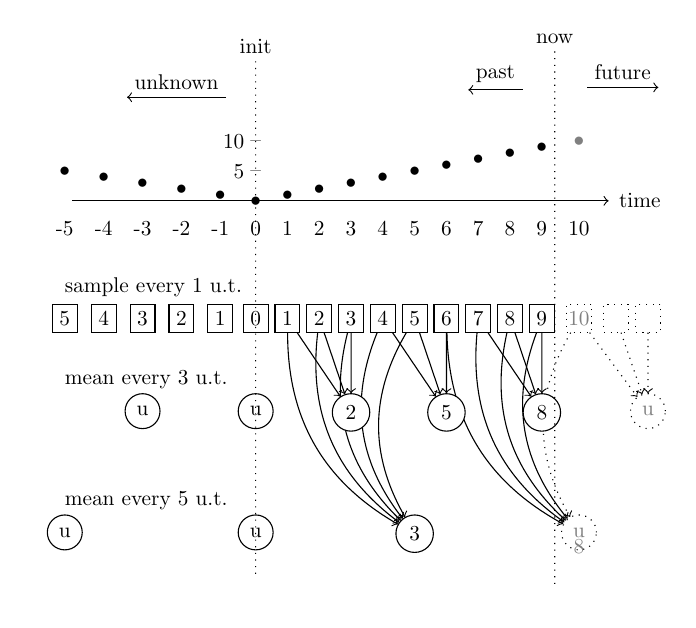
\begin{tikzpicture}[scale=0.77, every node/.style={transform shape}]

  %referencia
  \node (-6) {};

  \foreach \x in {-5,...,12}
  {
    \pgfkeys{/pgf/number format/.cd,int trunc}
    \pgfmathparse{abs(\x)}
    \let\absx=\pgfmathresult
    \pgfmathparse{\x-1}
    \let\antx=\pgfmathresult
    %time
    \node[node distance=1mm] (\x) [right=of \antx] 
    {\ifnum\x<11 \x \else \phantom{9} \fi};

    %graph values
    \node [above=\absx mm of \x] 
    {\ifnum\x=10 \color{gray} \fi \ifnum\x<11 $\bullet$ \fi};    

    %values
    % \node[rectangle,draw] (s\x) [below=of \x] 
    % {\ifnum\x<10 \pgfmathprintnumber{\absx} \else \phantom{9} \fi};
    \ifnum\x<10
    \node[rectangle,draw] (s\x) [below=of \x] 
    {\pgfmathprintnumber{\absx}};
    \else
    \node[rectangle,dotted,draw] (s\x) [below=of \x] 
    {\phantom{9}};
    \fi
  }

  \node [below=of 10] {\color{gray}10}; 
  

  
  %rd: 5s |inf| mean
  \node [circle,draw] (rd5-5) [below=3cm of s-5] {u};
  \node [circle,draw] (rd50) [below=3cm of s0] {u};
  \node [circle,draw] (rd55) [below=3cm of s5] {3};
  \node [circle,dotted,draw] (rd510) [below=3cm of s10] {\color{gray}u};
  \node [below=3.3cm of s10] {\color{gray}8};
 
  \draw[->,bend right] (s5) to (rd55);
  \draw[->,bend right] (s4) to (rd55);
  \draw[->,bend right] (s3) to (rd55);
  \draw[->,bend right] (s2) to (rd55);
  \draw[->,bend right] (s1) to (rd55);

  \draw[->,dotted,bend right] (s10) to (rd510);
  \draw[->,bend right] (s9) to (rd510);
  \draw[->,bend right] (s8) to (rd510);
  \draw[->,bend right] (s7) to (rd510);
  \draw[->,bend right] (s6) to (rd510);

  
  %rd: 3s |inf| mean
  \node [circle,draw] (rd3-3) [below=of s-3] {u};
  \node [circle,draw] (rd30) [below=of s0] {u};
  \node [circle,draw,fill=white] (rd33) [below=of s3] {2};
  \node [circle,draw,fill=white] (rd36) [below=of s6] {5};
  \node [circle,draw,fill=white] (rd39) [below=of s9] {8};
  \node [circle,dotted,draw] (rd312) [below=of s12] {\color{gray}u};

  \draw[->] (s3) to (rd33);
  \draw[->] (s2) to (rd33);
  \draw[->] (s1) to (rd33);

  \draw[->] (s6) to (rd36);
  \draw[->] (s5) to (rd36);
  \draw[->] (s4) to (rd36);

  \draw[->] (s9) to (rd39);
  \draw[->] (s8) to (rd39);
  \draw[->] (s7) to (rd39);

  \draw[->,dotted] (s12) to (rd312);
  \draw[->,dotted] (s11) to (rd312);
  \draw[->,dotted] (s10) to (rd312);



  %eixos
  \node (et0) [above=1mm of -5] {};
  \node (et12) [above=1mm of 11] {};
  \node [right=-2mm of et12] {time};
  \draw[->] (et0) to (et12);
  \node (y5) [above=5mm of 0] {--};
  \node [left=-1.5mm of y5] {5};
  \node (y10) [above=10mm of 0] {--};
  \node [left=-1.5mm of y10] {10};

  \node (inici) [above=4cm of s0] {init};
  \node (inici2) [below=4cm of s0] {};
  \draw[-,dotted] (inici) to (inici2);

  \node (fi) [above=4.4cm of s9.east] {now};
  \node (fi2) [below=4.4cm of s9.east] {};
  \draw[-,dotted] (fi) to (fi2);


  \node (fut) [below right=1mm and 1mm of fi] {future};
  \draw[->] (fut.south west) to (fut.south east);

  \node (pas) [below left=1mm and 1mm of fi] {past};
  \draw[->] (pas.south east) to (pas.south west);

  \node (unk) [below left=1mm and 1mm of inici] {unknown};
  \draw[->] (unk.south east) to (unk.south west);



  \node [above=0cm of s-5] {\makebox[0cm][l]{sample every 1 u.t.}};
  \node [below=0.5cm of s-5] {\makebox[0cm][l]{mean every 3 u.t.}};
  \node [below=2.5cm of s-5] {\makebox[0cm][l]{mean every 5 u.t.}};


\end{tikzpicture}



%%% Local Variables:
%%% TeX-master: "../main"
%%% ispell-local-dictionary: "british"
%%% End:

  \caption{Multiresolution snapshot diagram with regular sampling}
  \label{fig:mtsms:sequence}
\end{figure}


% \begin{figure}[tp]
%   \centering
%   %\usetikzlibrary{positioning}
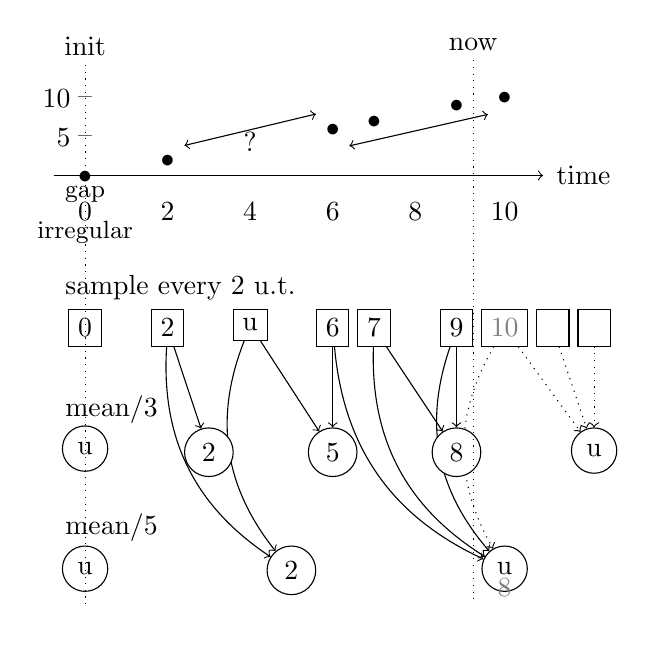
\begin{tikzpicture}

  \node[node distance=1mm] (0) {0};
  \node[node distance=1mm] (-1) [left=of 0]{\phantom{9}};
  \node[node distance=1mm] (1) [right=of 0] {\phantom{1}};
  \node[node distance=1mm] (2) [right=of 1] {2};
  \node[node distance=1mm] (3) [right=of 2] {\phantom{3}};
  \node[node distance=1mm] (4) [right=of 3] {4};
  \node[node distance=1mm] (5) [right=of 4] {\phantom{5}};
  \node[node distance=1mm] (6) [right=of 5] {6};
  \node[node distance=1mm] (7) [right=of 6] {\phantom{7}};
  \node[node distance=1mm] (8) [right=of 7] {8};
  \node[node distance=1mm] (9) [right=of 8] {\phantom{9}};
  \node[node distance=1mm] (10) [right=of 9] {10};
  \node[node distance=1mm] (11) [right=of 10] {\phantom{9}};
  \node[node distance=1mm] (12) [right=of 11] {\phantom{9}};


  \node [above=0 mm of 0] {$\bullet$}; 
  \node [above=2 mm of 2] (v2) {$\bullet$}; 
  \node [above=4 mm of 4] {?}; 
  \node [above=6 mm of 6] (v6) {$\bullet$}; 
  \node [above=7 mm of 7] {$\bullet$}; 
  \node [above=9 mm of 9] {$\bullet$}; 
  \node [above=10 mm of 10] (v10) {$\bullet$}; 


  \node[rectangle,draw] (s0) [below=of 0] {0};
  \node[rectangle,draw] (s2) [below=of 2] {2};
  \node[rectangle,draw] (s4) [below=of 4] {u};
  \node[rectangle,draw] (s6) [below=of 6] {6};
  \node[rectangle,draw] (s7) [below=of 7] {7};
  \node[rectangle,draw] (s9) [below=of 9] {9};
  \node[rectangle,draw] (s10) [below=of 10] {\color{gray}10};
  \node[rectangle,draw] (s11) [below=of 11] {\phantom{9}};
  \node[rectangle,draw] (s12) [below=of 12] {\phantom{9}};


  \draw[<->] (v2.north east) to (v6.north west)
  node [above,sloped,midway] {\small gap};

  \draw[<->] (v6.south east) to (v10.south west)
  node [below,sloped,midway] {\small irregular};

  
  %rd: 5s |inf| mean
  \node [circle,draw] (rd50) [below=4cm of 0] {u};
  \node [circle,draw] (rd55) [below=4cm of 5] {2};
  \node [circle,draw] (rd510) [below=4cm of 10] {u};
  \node [below=4.3cm of 10] {\color{gray}8};
 
  \draw[->,bend right] (s4) to (rd55);
  \draw[->,bend right] (s2) to (rd55);

  \draw[->,dotted,bend right] (s10) to (rd510);
  \draw[->,bend right] (s9) to (rd510);
  \draw[->,bend right] (s7) to (rd510);
  \draw[->,bend right] (s6) to (rd510);

  
  %rd: 3s |inf| mean
  \node [circle,draw] (rd30) [below=of s0] {u};
  \node [circle,draw,fill=white] (rd33) [below=2.5cm of 3] {2};
  \node [circle,draw,fill=white] (rd36) [below=2.5cm of 6] {5};
  \node [circle,draw,fill=white] (rd39) [below=2.5cm of 9] {8};
  \node [circle,draw] (rd312) [below=2.5cm of 12] {u};

  \draw[->] (s2) to (rd33);

  \draw[->] (s6) to (rd36);
  \draw[->] (s4) to (rd36);

  \draw[->] (s9) to (rd39);
  \draw[->] (s7) to (rd39);

  \draw[->,dotted] (s12) to (rd312);
  \draw[->,dotted] (s11) to (rd312);
  \draw[->,dotted] (s10) to (rd312);



  %eixos
  \node (et0) [above=1mm of -1] {};
  \node (et12) [above=1mm of 11] {};
  \node [right=-2mm of et12] {time};
  \draw[->] (et0) to (et12);
  \node (y5) [above=5mm of 0] {--};
  \node [left=-1.5mm of y5] {5};
  \node (y10) [above=10mm of 0] {--};
  \node [left=-1.5mm of y10] {10};

  \node (inici) [above=3.1cm of s0] {init};
  \node (inici2) [below=3.3cm of s0] {};
  \draw[-,dotted] (inici) to (inici2);

  \node (fi) [above=3.4cm of s9.east] {now};
  \node (fi2) [below=3.5cm of s9.east] {};
  \draw[-,dotted] (fi) to (fi2);


  % \node (fut) [below right=1mm and 1mm of fi] {future};
  % \draw[->] (fut.south west) to (fut.south east);

  % \node (pas) [below left=1mm and 1mm of fi] {past};
  % \draw[->] (pas.south east) to (pas.south west);

  \node [above=0cm of s0] {\makebox[0.5cm][l]{sample every 2 u.t.}};
  \node [below=0.5cm of s0] {\makebox[0.5cm][l]{mean/3}};
  \node [below=2cm of s0] {\makebox[0.5cm][l]{mean/5}};

\end{tikzpicture}



%%% Local Variables:
%%% TeX-master: "../main"
%%% ispell-local-dictionary: "british"
%%% End:

%   \caption{Multiresolution snapshot diagram with irregular sampling}
%   \label{fig:mtsms:sequence-irregular}
% \end{figure}



At the bottom of Figure~\ref{fig:mtsms:sequence} there is a diagram
showing the multiresolution action. The first row shows the numerical
time series' values corresponding to the above plot; the time series
is sampled every one unit of time. The second and the third row show a
particular schema of a multiresolution database consisting in two time
resolutions for the time series: one computes the mean of the sampled
values every three u.t.\ and the other computes the mean every five
u.t. In this example, computing the mean acts as selecting information
by aggregate statistics. All data stored before zero time is unknown
(\emph{u}) as has not been acquired. For the future values it is also
marked as \emph{u} until time advances.

The arrows of the figure show that every three sampled values a mean
is stored and, independently, every five values another mean is
stored. For the future values, dashed arrows show that if time
advances one u.t.\ then value 10 is sampled and the mean for time 10
can be computed resulting 8 but not yet the mean for time 12.

% Fig.~\ref{fig:mtsms:sequence-irregular} is essentially the same but
% showing two possible monitoring irregularities: a gap and a time
% disruption. In other words, we want to sample the time series every 2
% u.t.\ but first for some reason it can not be done in time 4 and
% second the sampling clock is disrupted and samples are done in time 7
% and 9 instead of 8. The resulting stored time schema is the same: on
% time resolution every 3 u.t.\ and the other every 5 u.t.; that is,
% without time disruptions. The resulting stored values are computed
% from the known sampled values, some coincide with
% fig.~\ref{fig:mtsms:sequence} whereas some differ specially in the
% gap. A better function than mean would solve this, we extend this
% further in section~\ref{sec:model:interpolador}.



%%% Local Variables:
%%% TeX-master: "main"
%%% ispell-local-dictionary: "british"
%%% End:

%  LocalWords:  multiresolution TSMS MTSMS


%-- ART --
\chapter{Estat actual}
\label{cap:estat}


SGBD: sistema de gestió de bases de dades

SGBDR: SGBD relacional

SGST: SGBD per sèries temporals



%Estat de l'art

% * no n'hi ha d'específic del tema, potser el que més s'hi assembla són els SGST que hi ha (Cougar, RRDtool, ...)

% * Hi ha temes colaterals (monitoratge,anàlisis)

% * Temes para\l.lels que ens serveixen d'inspiració (SGBD relacionals)

%Cal introduir bé el forat de coneixement que hi ha en els SGST. Forat entre les sèries temporals i els SGBD.



%Capítol:

% * Sèries temporals
  
%   - mineria
%   - aplicacions
%   - monitoratge de sèries temporals i problemes
%      * censura
%      * mostreig

%   - sgst: 
%       ficar aquí els sgbd per sèries temporals i més endavant ja es parlarà dels sgbd en general i com modelar-los i implementar-los.


% * SGBD
%  - model relacional
%  - implementacions
%  - temporal data


  % * Sèries temporals (històrics, predicció, diagnosis, prognosis, etc.)
  % * Mostreig: docs quan període de mostreig no regular
  % * Bases de dades (docs d'emmagatzematge quan la memòria és finita, docs quan període de mostreig no és regular, altres sistemes semblants (comercials,prototips))




% El capítol comença resumint l'estat de les sèries temporals en aquest camp de mineria; és a dir d'emmagatzematge i tractament. A continuació es llisten algunes aplicacions informàtiques que han implementat models de la mineria de sèries temporals. Finalment, es descriu l'estat actual de l'aplicació RRDtool, la qual també es classifica en aquest camp.

% This paper focuses on Data Base Management Systems (DBMS) that store
% and treat data as time series.   Other DBMS are not adequate for these cases as they do not have enough facilities to manage and retrieve time series
% information \parencite{schmidt95}.

% DBMS are based from formal models that define the objects and
% operations of the abstract machine to which users interact, such is
% the relational model \parencite{date}. TSMS lack a consolidated formal
% model, although special properties and requirements for a TSMS
% have been proposed \parencite{dreyer94}.








%%% Local Variables: 
%%% mode: latex
%%% TeX-master: "main"
%%% End: 

% LocalWords:  monitoratge

\todo{dir}
dir que en el nostre model no ens ocupem de l'etapa d'adquisició/mostreig de les sèries temporals sinó que tenim unes mesures que s'han capturat d'alguna manera. Si bé cal destacar que alguns SGST sí que influeixen al procés d'adquisició, per exemple poden controlar obtenir més mostres si veuen coses rares, no mostrejar més si és tranquil, canviar paràmetres, etc.


\todo{}
explicar el data mining com a background per a les oepracions que es poden fer amb les sèries temporals: pattern search, similiraties, etc.

\section{Sèries temporals}





Una sèrie temporal és un conjunt de valors cadascun dels quals té
associat un instant de temps diferent.  Tradicionalment s'anomenen
sèries temporals tot i que també s'accepta la denominació de
seqüències temporals, per exemple a \cite{last:hetland}.

Les sèries temporals s'emmarquen dins l'àmbit més genèric del que es
coneix com a \emph{dades temporals}. Les dades temporals són
co\l.leccions de dades arbitràries que estan associades a la dimensió
temps.  Dins del concepte de dades temporals s'hi encabeixen
co\l.leccions de dades de diversa natura. En funció de com un valor
queda vinculat amb el temps, es poden diferenciar dues
categories \parencite{assfalg08:thesis}.
\begin{enumerate}
\item La primera la formen les sèries temporals tal i com s'han
  definit prèviament, en la qual la dada està associada a un instant
  de temps.
\item La segona, que anomena \emph{bitemporal data}, la formen
  co\l.leccions de dades en que cada element té dos atributs
  temporals: el rang de validesa, que indica l'intèrval de temps en
  que la dada és vàlida, i el temps de transacció, que indica quan es
  va desar la dada a la base de dades.  
  %\citeauthor{assfalg08:thesis} a \cite{assfalg08:thesis} assegura que aquesta categoria de dades temporals es poden expressar en termes de la primera.\todo{Teresa5}
\end{enumerate}
Aquestes dues categories de dades temporals, tot i tenir aspectes en
comú, no poden ser tractades amb els mateixos
sistemes, \parencite{schmidt95}.


Les sèries temporals s'utilitzen en camps molt diversos i amb
objectius molt diferents. L'ús generalitzat és per a l'anàlisi i la
comprensió del comportament temporal de variables. L'evolució d'una
sèrie temporal es pot representar amb un model. Aquests models, en
l'àmbit de l'enginyeria, permeten realitzar tasques relacionades amb
validació de dades, diagnòstic i prognosis.  Per exemple, trobem
aplicacions de sèries temporals en el camp de l'avaluació de la
degradació de components \parencite{yu11}, anàlisi de l'estat dels
sensors d'un vaixell \parencite{palmer07}, validació i reconstrucció
de dades en xarxes de distribució d'aigua \parencite{quevedo10},
classificació de valors econòmics \parencite{dreyer95}, optimització
de la planificació semafòrica \parencite{last11}, estimació del temps
de viatge en autopistes \parencite{soriguera10} o transmissió
d'informació en xarxes de
sensors \parencite{jainagrawal05,yaogehrke02}.
\todo{també sèries temporals van de bracet amb GIS, exemple en dades hidrològiques [bollaert06:thesis]}


Aquest apartat té com a objectiu mostrar l'estat de l'art dels
principals processos vinculats en el treball amb sèries temporals. A
tal efecte s'organitza en tres subapartats.
 

El primer subapartat se centra en l'adquisició de dades. El primer
requeriment d'una sèrie temporal és l'adquisició de dades. Els
sistemes de monitoratge s'encarreguen de recollir dades dels sensors,
periòdicament o en base a esdeveniments.  Els problemes que es donen
durant l'adquisició generen defectes específics en les sèries
temporals que cal analitzar i tractar convenientment.


El segon subapartat tracta de l'anàlisi de sèries temporals, que és
la formalització de les tècniques que s'utilitzen per extreure
informació. A vegades aquesta extracció també es coneix com
descobriment de coneixement i s'emmarca dins de l'inte\l.ligència
artificial.


El tercer subapartat es dedica als sistemes d'emmagatzemat de sèries
temporals. L'emmagatzematge de les dades i la implementació de les
tècniques d'anàlisi té lloc en els sistemes de gestió de bases de
dades. Aquests s'encarreguen de l'organització correcte de la
informació i de respondre a les operacions de consulta. Les sèries
temporals necessiten un tractament específic per part d'aquests
sistemes.






\subsection{Adquisició de sèries temporals}

Els sistemes de monitoratge són un part important d'interacció entre
un procés i els usuaris, entenent com a procés qualsevol sistema
físic, químic, ambiental, etc.\ del qual es pugui recollir informació
continuada, ja sigui de forma periòdica o en funció
d'esdeveniments. Principalment, aquests sistemes s'encarreguen de
recollir dades, conèixer l'estat actual del procés i informar a
l'usuari. Els sistemes de monitoratge constitueixen la part principal
dels sistemes SCADA (\emph{Supervisory Control And Data
  Acquisition}). Un SCADA és el sistema encarregat de recollir i
centralitzar les dades de manera periòdica en el temps.



\begin{figure}[tp]
  \begin{center}
    \scriptsize 
    ../../../imatges/aplicacions/monitoratge.tex
  \end{center}
  \caption{Sistema de monitoratge: de l'adquisició de dades fins a informar l'usuari}
  \label{fig:sistema_monitoratge}
\end{figure}


El monitoratge es pot dividir en diferents blocs principals, els quals
es mostren a la \autoref{fig:sistema_monitoratge}. Un monitor
adquireix dades dels sensors. Les dades poden ser valors de mesures o
estats del procés adquirits com a esdeveniments. Fent referència a la
classificació de dades temporals de \textcite{assfalg08:thesis}, en
general les mesures es poden entendre com a sèries temporals i els
esdeveniments com a dades bitemporals.

En el cas de sistemes controlats o automatitzats, les dades adquirides
poden ser utilitzades per comandar o modificar el funcionament del
procés. Aleshores s'incideix en diferents nivells des de llaços de
control modificant directament un accionament, fet que no sol ser
habitual ja que els llaços de control solen realitzar-se els sistemes
electrònics que resideixen prop dels sistemes controlats, fins a
gestió de modes de funcionament i coordinació entre màquines, fet més
habitual.

L'ús generalitzat dels sistemes de monitoratge és el de proporcionar
informació de l'estat actual del procés. També disposen de la
possibilitat de generar alarmes senzilles com per exemple que no s'han
pogut adquirir les dades o que el sensor ha assolit un valor
crític. Per a usuari ens referim tant a un usuari humà com a un altre
sistema supervisor dotat amb inte\l.ligència artificial.

Per a càlculs més complicats amb les dades, els sistemes de
monitoratge utilitzen sistemes de gestió de bases de dades
(SGBD). Mitjançant els SGBD, s'emmagatzemen les dades en bases de
dades i posteriorment l'usuari les consulta per observar els històrics
o per obtenir informació i elaborar coneixement a partir de les dades
emmagatzemades.

La \autoref{fig:sistema_monitoratge} presenta una visió centralitzada
de l'adquisició de dades. Ara bé, els sistemes de monitoratge
internament poden tenir estructura distribuïda quan els sensors tenen
suficient capacitat de processament, com per exemple les xarxes de
sensors. En aquests casos els monitors cedeixen parts al sensors,
sobretot pel que fa als SGBD que passen a tenir un paper més rellevant
en la comunicació.


Un dels camps recents on l'adquisició de sèries temporals hi juga un
paper fonamental és el de les xarxes de sensors. L'abaratiment del
maquinari permet monitorar el procés amb grans quantitats de sensors
inte\l.ligents \parencite{jainagrawal05,yaogehrke02}, els quals tenen
processador i ràdio incorporats però tenen recursos limitats pel que
fa a transmissió, energia i processament i estan sotmesos a la
incertesa dels sensors. Així doncs, el problema de les xarxes de
sensors rau en estudiar l'ús eficient d'aquests recursos, pel qual
actualment trobem dues propostes.  Una solució consisteix en
transmetre la informació a un node central comprimint-la tant amb
agregacions (estadístics) com amb
aproximacions \parencite{deligiannakis07}.  Una altra solució
consisteix en tenir les dades distribuïdes en diferents sensors i
decidir com s'ha de resoldre cada consulta tenint en compte que el
processament local és més barat que la
comunicació \parencite{yaogehrke02,gehrkemadden04,bonnet01}.

\todo{el tema d'agregar informació en xarxes de sensors és interessant, potser hauria de tenir una secció pròpia}

\todo{citar kim12}:
Research Article
Aggregate Queries in Wireless Sensor Networks
Jeong-Joon Kim,1 In-Su Shin,1 Yan-Sheng Zhang,2 Dong-Oh Kim,3 and Ki-Joon Han1
Hindawi Publishing Corporation
International Journal of Distributed Sensor Networks
Volume 2012, Article ID 625798, 15 pages
doi:10.1155/2012/625798





\subsubsection{Problemes en el monitoratge}

Els sistemes de monitoratge habitualment presenten problemes derivats
de la reco\l.lecció de dades. Principalment distingim tres problemes.

\todo{parlar també del problema de la sincronització de rellotges}
\textcite[cap.~3]{kopetz11:realtime}


\begin{enumerate}
\item El primer problema és la gestió d'una quantitat enorme de dades. 

Un sistema de monitoratge recull una gran quantitat de dades. Ara bé, l'usuari només en pot observar una petita part sincronitzat (\emph{online}) amb el procés i les dades emmagatzemades esdevenen massa grans per a ser processades posteriorment \parencite{keogh97}. No obstant, les dades han de ser analitzades ja que contenen informació interessant per a les aplicacions de les sèries temporals descrites a l'apartat anterior. S'observa que en el context de monitoratge les dades recollides es poden considerar com a sèries temporals ja que abstractament són una co\l.lecció de mesures.


\item El segon problema és el de la necessitat de censurar les dades, és a dir validar que les dades siguin correctes i en cas contrari rebutjar-les o reconstruir-les. 

\textcite{quevedo10} mostren la quantitat d'informació que hi ha en els sistemes complexos de telecontrol. Aquesta informació s'obté de diversos sensors distribuïts pel camp de mesura.
En el moment de reco\l.lecció de dades apareixen dos problemes: valors que en un instant de temps prefixat no s'han pogut recollir i valors que són falsos. En el procés de gestió de dades no es poden emmagatzemar les dades amb aquests dos tipus de problema ja que aleshores els registres històrics serien inconsistents. 
Així doncs, cal comprovar que les dades emmagatzemades són correctes, mitjançant un procés de validació, i modificar-les en el cas que siguin falses, mitjançant un procés de reconstrucció que estimi els valors correctes. Per exemple, \citeauthor{quevedo10} apliquen aquests processos de validació i reconstrucció a xarxes de distribució d'aigua.


\item El tercer problema es dóna quan el període de mostreig no és regular, és a dir que les dades no es recullen de manera uniforme en el temps, però les aplicacions no ho contemplen o volen treballar amb dades a intervals regulars, també anomenat dades equi-espaiades.

Una causa de la irregularitat es deu a que els sistemes de monitoratge informàtics sovint no són capaços de complir amb exactitud el temps de mesura sinó que presenten una certa variació, ja sigui deguda a retards en els sensors, les comunicacions o la planificació del monitoratge amb altres tasques concurrents del sistema operatiu. Aquesta causa, però, es pot atenuar si els sensors envien el temps de mesura juntament amb el valor mesurat. Aleshores, el problema recau en la sincronització dels rellotges dels sensors. \todo{busca jitter en el periodic sampling de control}

Una altra causa es deu a que l'adquisició de dades prové de processos sotmesos a sistemes de control, els quals prenen el control de l'adquisició de dades. És a dir, el sistema de monitoratge ha d'obeir a les restriccions de temps imposades pels llaços de control. Aquestes restriccions són especialment crítiques en els sistemes de control en temps real ja que, aleshores, el sistema de monitoratge no pot imposar restriccions de temps diferents de les que s'han calculat per als llaços de control.  \textcite{lozoya08} mostren que s'ha de vigilar amb les entrades i sortides de les tasques periòdiques als sistemes en temps real. L'actuació dels sistemes de control es degrada quan no es té en compte que les operacions d'entrada i sortida estan subjectes a fluctuacions degudes al mostreig i a latències. Aquest problema afecta als sistemes de monitoratge en dues vessants.
Per una banda, els sistemes de monitoratge tenen una part de l'adquisició controlada per les aplicacions de control en temps real i per tant el període de mostreig resultant que veu el monitor no és regular. 
Per altra banda, les aplicacions que analitzen les dades obtingudes del monitoratge poden veure com la seva actuació es degrada si no consideren que l'adquisició de dades és irregular, el qual és similar a la regressió que s'observa \parencite{lozoya08} quan en el disseny d'un controlador discret es considera que es mostreja i s'actua periòdicament però en la implementació amb un sistema en temps real aquest pot fluctuar la periodicitat.
\todo{event based sampling/control}

\end{enumerate}



En conclusió, per tal de gestionar la complexitat derivada de la recollida de dades i també la complexitat de les consultes posteriors per part de l'usuari, els sistemes de monitoratge es recolzen en sistemes de gestió de bases de dades per gestionar l'emmagatzematge de les dades i la recuperació d'informació.





\subsection{Anàlisi de sèries temporals}

\todo{dir que una aplicació emergent és l'anàlisi de dades en temps real/en línia amb el procés per a prendre decisions}

L'anàlisi de sèries temporals consisteix en l'aplicació de
metodologies i d'algoritmes que permeten tasques com per exemple
l'extracció de característiques o obtenció de models.  Aquestes
tècniques es recullen en el que es coneix amb el nom de mineria de
sèries temporals (\emph{time series data mining}). La mineria de
dades, en la qual s'inscriu la de sèries temporals, és l'estudi
d'algoritmes específics per a extreure patrons de comportament de les
dades i s'inclou com un pas del procés general de descobriment de
coneixement a les bases de dades (\emph{knowledge discovery in
  databases}) \parencite{fayyad96,last01}.
% [M. E. Mueller, Relational Knowledge Discovery, Cambridge 2012. sec1.1p7]
%knowledge discovery: process of extracting new knowledge from a set of data about that set of data, This means that the acquisition of new lnowledge requires us to build a new model of the data.
% Data mining: refers mostly to the extraction of parts of information with respect to a given model. 
%Exemple: correlació, si dues coses tenen correlació no vol dir que necessàriament hi hagi una dependència causal entre les dades.

Actualment, les sèries temporals es consideren com un dels deu problemes
prioritaris en la mineria de dades \parencite{yangwu06}. Tal com
esmenta \textcite{fu11} en un article recent, la recerca en mineria de
sèries temporals s'ha incrementat en la darrera dècada. L'objectiu
principal és reduir la mida de les sèries temporals per tal de
disminuir el temps de processat de les dades.  \citeauthor{fu11}
resumeix l'estat actual de la mineria de sèries temporals de forma
exhaustiva i conclou que encara queden molts problemes per investigar
i resoldre. La recerca en tasques de mineria ha estat intensa però es
necessita millorar la representació de sèries temporals, ja que es
considera el pas que redueix la mida de les dades.

Segons \textcite{keogh02}, les quatre tasques que centren l'atenció de
la recerca actual de sèries temporals són l'indexat (\emph{indexing}),
que treballa amb una estructura comprimida de les dades; l'agrupament
(\emph{clustering}), que agrupa les dades segons la similitud entre
elles per tal de descobrir patrons; la classificació
(\emph{classification}), que etiqueta les dades segons les
característiques que presentin; i la segmentació
(\emph{segmentation}), que parteix una sèrie temporal en
subseqüències.  A més, \citeauthor{keogh02} comparen alguns algoritmes
experimentals duts a terme en aquests camps per diversos
autors. Recomanen a la comunitat de mineria de sèries temporals que
segueixi el seu estudi com a punt de referència per avaluar el
rendiment d'algoritmes similars.

Un pas comú previ a les quatre tasques anteriors és el de representació de la sèrie temporal. Les sèries temporals són discretes, són valors en punts de temps discrets, i la representació és el model de funció que aproxima la sèrie temporal a la seva naturalesa contínua original. La mineria de sèries temporals aprofita la representació per reduir la mida de les sèries temporals.
La representació de sèries temporals a trossos lineals (PLR, \emph{Piecewise Linear Representation}) \parencite{keogh97,keogh98} {é}s la més habitual actualment per ser més propera als usuaris ja que la visió de l'ésser humà segmenta les corbes en línies rectes.
Després de definir la PLR, \textcite{keogh00,keogh01} exploren altres representacions de sèries temporals per tal de reduir la mida d'una sèrie temporal i poder-la indexar més fàcilment. Proposen dues tècniques eficients en el càlcul: la \emph{Piecewise Aggregate Aproximation} i la \emph{Adaptive Piecewise Constant Approximation}, ambdues basades en la representació a trossos constants de la sèrie temporal. 
D'aquestes dues tècniques, \citeauthor{keogh00,keogh01} conclouen que mantenen una bona aproximació a la sèrie temporal i que a més  tenen molt menys cost de càlcul que altres de més complicades, com ara la \emph{Discrete Fourier Transform},  la  \emph{Singular Value Decomposition} o la \emph{Discrete Wavelet Transform}.

\todo{arreglar perquè quedi ben explicat; després en el model fem menció d'aquestes representacions}

\todo{potser posar-ho a estat de l'art tot això?}


In the design of the attribute interpolation function we can interpret
a time series in different ways, that is what we call the
representation of a time series. Keogh et al.\ \cite{last:keogh} cite
some possible representations for time series such as \emph{Fourier
  Transforms}, \emph{Wavelets}, \emph{Symbolic Mappings} or
\emph{Piecewise Linear Representation} (PLR). This last is remarked as
the most used owing to the most common representation is with linear
functions \cite{keogh01}.


\todo{last01} també fa una mena d'agregacions amb l'objectiu de trobar un a funció que s'aproximi a un interval de la sèrie temporal. Seria un mètode d'agregació amb aproximació?


\paragraph{Representació de sèries temporals}

\textcite{last:keogh}, cita vàries representacions per les sèries temporals com per exemple \emph{Fourier Transforms}, \emph{Wavelets}, \emph{Symbolic Mappings} o \emph{Piecewise Linear Representation} (PLR), però assenyala aquesta última com la representació més utilitzada. 
La PLR, funció definida a trossos lineal, és l'aproximació d'una sèrie temporal $S$, de llargada $n$, amb $K$ segments rectes. Els segments podrien ser polinomis de qualsevol grau, però la manera més comuna de representar sèries temporals és amb funcions lineals, segons Keogh, \cite{keogh02}.
Per aproximar el segment $S(t_a,t_b]$ d'una sèrie $S$, Keogh defineix dues tècniques: interpolació lineal, la recta que connecta $t_a$ i $t_b$, i regressió lineal, la millor recta que aproxima per mínims quadrats el segment entre $t_a$ i $t_b$.

Però també es pot representar una sèrie temporal amb una funció graó (\emph{step} o \emph{staircase function}); és a dir, amb una funció definida a trossos constant (\emph{piecewise constant representation}).
La representació a trossos constant és utilitzada en electrònica als convertidors digital-analògic (DAC, \emph{digital-to-analog converter}). En aquest cas, un senyal discret es considera una sèrie temporal i per reconstruir el senyal continu típicament s'aplica el model de \emph{zero-order hold}, equivalent a la representació a trossos constant,  o el de \emph{first-order hold},  equivalent a la representació a trossos lineal.
El model de \emph{zero-order hold} consisteix en mantenir constant cada valor fins al proper. S'obté una representació a trossos constant que en electrònica s'anomena seqüència de pulsos rectangulars (\emph{rectangular pulses}).

%http://en.wikipedia.org/wiki/Piecewise

%http://ca.wikipedia.org/wiki/Funció_definida_a_trossos

%http://en.wikipedia.org/wiki/Rectangular_function

%http://en.wikipedia.org/wiki/Step_function

% Piecewise Aggregate Approximation (PAA) \cite{keogh00}: aproxima una sèrie temporal partint-la en segments de la mateixa mida i emmagatzemant la mitjana dels punts que cauen dins del segment. Redueix de dimensió $n$ a dimensió $N$

% Adaptive Piecewise Constant Approximation (APCA) \cite{keogh01}: com el PAA però amb segments de mida variable.




\subsection{Emmagatzematge i gestió de sèries temporals}


Els sistemes de gestió de bases de dades (SGBD) són els sistemes informàtics que s'encarreguen d'emmagatzemar informació i de permetre a l'usuari consultar-la. A la secció \ref{sec:art:sgbd} es descriu com es formalitzen els SGBD, en aquest apartat ens centrarem en les necessitats que tenen les sèries temporals dels SGBD.


Les sèries temporals es diferencien d'altres tipus de dades en que els seus valors són dependents d'una variable: el temps. Com a conseqüència, qualsevol SGBD que hi vulgui tractar no ho pot fer de manera independent pels valors i pel temps; ha de conservar la coherència temporal.

Per poder aplicar les tècniques d'anàlisis de les sèries temporals de manera eficient cal disposar de SGBD específics. 
Durant l'última dècada, el maquinari informàtic ha millorat tant des del punt de vista tecnològic com de l'econòmic \parencite{deligiannakis07}, el qual ha facilitat l'adquisició de dades, per exemple amb xarxes de sensors, i alhora ha ampliat la capacitat per emmagatzemar les dades. 
Per tant, el volum de dades a tractar  en els SGBD cada cop esdevé més crític.

 
En els SGBD, el problema de grans quantitats de dades també es troba en altres camps com demostren \textcite{mylopoulos96} sobre la necessitat de grans bases de dades de coneixement. Els SGBD que tracten amb aquestes dades s'anomenen \emph{very large databases} (VLDB) i han de construir, accedir i gestionar la quantitat de dades de manera eficient.

\textcite{ogras06} consideren que les aproximacions que fan les VLDB
estan pensades per a bases de dades estàtiques. No obstant, observen
que les sèries temporal normalment són dinàmiques, és a dir de
naturalesa contínua i de mida no fitada. Conseqüentment, conclouen que
les solucions tradicionals, les quals analitzen a posteriori i sense
tenir en compte l'ordre, no es poden aplicar a causa de l'arribada
seqüencial i contínua de les dades.  Com a solució proposen resumir
dinàmicament les sèries temporals amb les tècniques de compressió que
s'apliquen en altres aplicacions on hi ha bases de dades grans.




\textcite{dreyer94} proposen desenvolupar SGBD que implementin operacions específiques per les sèries temporals, aleshores els anomenen sistemes de gestió de bases de dades per sèries temporals (SGST, \emph{time series database management systems}). Consideren que els altres SGBD no són adequats per tractar sèries temporals, tot i que després de comparar els SGBD per dades temporals i els SGST \parencite{schmidt95} troben que hi ha aspectes comuns entre els dos sistemes.
Els SGST estan optimitzats per gestionar les dades segons les operacions de temps i rotació, les quals són molt comunes en la gestió de les sèries temporals.  A més també cal controlar el creixement de la base de dades i la consulta ha de ser flexible i d'alta velocitat \parencite{keogh10:isax}. 
No obstant, fins a on coneixem, les propietats d'un model de SGST no s'han investigat més enllà  ja que la recerca s'ha concentrat en tasques de mineria de dades. Per exemple \textcite{last01} estudien una metodologia general per descobrir coneixement en els SGST, tant pel que fa a 
patrons temporals %(groups of events ordered by time)
com a regles temporals%(cause-effect relationships between events)
, i breument noten l'existència del model \cite{dreyer94} pels SGST.


Altres estudis proposen tractar les sèries temporals com a tipus que tenen ordre, per exemple seqüències o matrius.

\textcite{seshadri96:thesis} proposa que les sèries temporals són un subconjunt de les seqüències i per tant el model i les operacions per les seqüències \parencite{seshadri95} serveixen per les sèries temporals. 
\textcite{bonnet01} utilitzen el model de seqüències en SGBD distribuïts per xarxes de sensors, aleshores l'estratègia de comunicació inclou agregacions de les sèries temporals en els sensors \parencite{demers03}.
També es relaciona el model de seqüències de les sèries temporals amb els \emph{data streams} \parencite{babcock02,jagadish95,ogras06}. Els \emph{data streams} són dades que arriben contínuament i amb ordre temporal i es modelen com una seqüència on només s'hi poden afegir elements. Aleshores les consultes poden ser contínues, és a dir cada cop que arriba una dada nova s'actualitza incrementalment la informació. Per les sèries temporals s'utilitza en el càlcul de correlacions i prediccions de forma incremental \parencite{yi00} i en la cerca de patrons \parencite{bai05}.
%Data Stream Management System (DSMS) is an extension of Data Base Management System  

\todo{tot i així sembla que el concepte de bases de dades científiques ja apareix des de fa força temps \cite{segev87:sigmod}} 
En els SGBD per matrius \emph{arrays} destaquen els anomenats sistemes
de gestió de bases de dades científiques, camp en el qual les sèries
temporals hi tenen un paper de primer
ordre \parencite{zhang11}. \textcite{stonebraker09:scidb} estudien les
necessitats d'aquests sistemes sobretot en l'àmbit de la
ciència. \textcite{kersten11} proposen un sistema molt semblant però a
més integren el seu llenguatge, anomenat SciQL (\emph{SQL for
  science applications}), amb la sintaxi de SQL (\emph{Structured Query Language},
vegeu apartat \ref{sec:estat:sgbdr}). \textcite{zhang11} exemplifiquen
detalladament l'ús de SciQL en les sèries temporals per a algunes de
les seves propietats: regularitat, interpolació i cerca de
correlacions.




\todo{big data}

\url{http://cacm.acm.org/magazines/2014/7/176204-big-data-and-its-technical-challenges/fulltext}



\subsubsection{Implementacions actuals}

Hi ha hagut vàries implementacions de sistemes específics per a sèries
temporals. Algunes són només l'aplicació d'un algoritme d'anàlisi per
un problema concret de sèries temporals però altres són més elaborades
i es defineixen com a SGBD per a sèries temporals.  En aquest apartat
resumim algunes aplicacions que considerem que implementem conceptes
dels SGST.



\begin{description}

\item[Calanda] \textcite{dreyer94} proposen els requeriments de propòsit específic que han de complir els SGST i basen el model en quatre elements estructurals bàsics: esdeveniments, sèries temporals, grups i metadades, a banda de les bases de dades per sèries temporals. Implementen un SGST anomenat Calanda \parencite{dreyer94b,dreyer95,dreyer95b} que té operacions de calendari, pot agrupar sèries temporals i respondre consultes simples i ho exemplifiquen amb dades econòmiques. A \cite{schmidt95} es compara Calanda amb els SGBD temporals que operen amb sèries temporals. 




\item[T-Time] \textcite{assfalg08:thesis} mostra un sistema que pot cercar similituds calculades com a distàncies entre sèries temporals. Principalment, dues sèries temporals es marquen com a similars si la seva distància és menor que un llindar en cada interval. A partir d'aquest mètode dissenya algoritmes eficients que implementa en un programa anomenat T-Time \parencite{assfalg08:ttime}.


 
\item[iSAX] \textcite{keogh08:isax,keogh10:isax} estudien l'anàlisi i l'indexat de co\l.lecions massives de sèries temporals. Descriuen que el problema principal del tractament rau en l'indexat de les sèries temporals i proposen mètodes per calcular-lo de manera eficient. El mètode principal que proposen està basat en l'aproximació a trossos constants de la sèrie temporal \parencite{keogh00}.  Ho implementen en una estructura de gestió de dades que anomenen \emph{indexable Symbolic Aggregate approXimation} (iSAX) \parencite{isax}. Les representacions de sèries temporals que s'obtenen amb aquesta eina permeten reduir l'espai emmagatzemat i indexar tant bé com altres mètodes de representació més complexos.




\item[TSDS]
\textcite{weigel10} noten la necessitat de mostrar les dades en tot el seu rang temporal i no només en un subconjunt com normalment s'ofereixen. Desenvolupen el paquet informàtic \emph{Time Series Data Server} (TSDS) \parencite{tsds} a on es poden introduir les dades de sèries temporals per posteriorment consultar-les per rangs temporals o aplicant-hi filtres i operacions.





\item[RRDtool]
RRDtool \parencite{rrdtool} {é}s un SGBD molt usat per la comunitat de programari lliure. Projectes en diversos camps l'utilitzen com a SGBD, en els quals hi ha sistemes de monitoratge professionals, també en l'àmbit de programari lliure, com Nagios/Icinga \parencite{nagios,icinga} o el Multi Router Traffic Grapher (MRTG) \parencite{mrtg}. Aquests monitors transfereixen a RRDtool la responsabilitat de gestionar l'emmagatzematge i d'operar amb les dades, i així es poden centrar en l'adquisició de dades i la gestió d'alarmes. 
En l'evolució de RRDtool hi ha dues millores destacables. En primer lloc, \textcite{lisa98:oetiker} va separar el sistema de gestió de RRDtool de MRTG i el va dissenyar amb una estructura característica de Round Robin. En segon lloc,  \textcite{lisa00:brutlag} va estendre RRDtool amb algoritmes de predicció i detecció de comportaments aberrants. 

Actualment, s'està estudiant l'eficiència i rapidesa de RRDtool a processar sèries temporals. \textcite{carder:rrdcached} ha dissenyat una aplicació, \emph{rrdcached}, que millora el rendiment de RRDtool amb la qual s'aconsegueix fer funcionar  simultàniament sistemes amb grans quantitats de bases de dades RRDtool \parencite{lisa07:plonka}. \textcite{jrobin} han dissenyat una adaptació de RRDtool anomenada \emph{JRobin}. 
Finalment, és destacable l'ús emergent de RRDtool en entorns d'experimentació, com és el cas de \textcite{zhang07} i \textcite{chilingaryan10} que hi emmagatzemen dades experimentals per posteriorment predir o validar-les.


\item[Cougar]
\textcite{cougar,fung02} proposen Cougar com un SGBD per xarxes de sensors (\emph{sensor database systems}). El sistema té dues estructures \parencite{bonnet01}: una basada en relacions per les característiques dels sensors i una basada en seqüències per les dades dels sensors, les quals són sèries temporals.
Les consultes es processen de manera distribuïda: cada sensor és un node amb capacitat de processament que pot resoldre una part de la consulta i fusionar-la amb les altres. D'aquesta manera es minimitza l'ús de comunicacions però l'estructura i estratègia de comunicació dels nodes esdevé una part crítica a configurar \parencite{demers03}.

\item[TinyDB]
Un altre prototip de SGBD per xarxes de sensors desenvolupat para\l.lelament a Cougar és TinyDB \parencite{tinyDB,madden05}. A part de les característiques descrites per Cougar, aquest sistema  modifica i s'implica en parts del procés d'adquisició de les dades com és el temps, la freqüència o l'ordre de mostreig. Per exemple donada una consulta que vol correlacionar les dades de dos sensors, el sistema indica als sensors implicats que han d'adquirir amb la mateixa freqüència.

\item[SciDB]
\textcite{stonebraker09:scidb} estudien els SGBD científiques amb models  de dades basats en matrius. Estan desenvolupant SciDB \parencite{scidb}, un SGBD productiu i optimitzat per treballar amb matrius.


\item[SciQL]
\textcite{kersten11} descriuen SciQL, un llenguatge per a SGBD científiques basades en matrius. Hi ha un prototip en desenvolupament de SciQL \parencite{sciql}.


\end{description}


%SETL http://setl.org/setl/ un llenguatge de programació d'alt nivell que té els conjunts i els mapes de primer ordre com a parts fonamentals. Els tipus bàsics són conjunts, conjunts desordenats i seqüències (també anomenades tuples). Els mapes són conjunts de parelles (tuples de mida dos). Les operacions bàsiques inclouen la pertinença, la unió, la intersecció, etc.


\todo{}


OpenTSDB \cite{deri12:tsdb_compressed_database}
\url{http://opentsdb.net/}
Han fet anàlisis del rendiment de RRDtool, MySQL i la seva implementació TSDB i conclouen que RRDtool és el que pitjor funciona per a sèries temporals. La seva implementació, TSDB, es basa en la compressió de dades. Assumeixen que les sèries temporals són regulars i totes tenen el mateix patró de mostreig, fet que els permet implementar les gestió de les sèries temporals de manera més senzilla.
\todo{Potser hauria de classificar els SGST segons si es basen en compressió de dades (aquest tsdb, iSAX..), en Round Robin (RRDtool), vectors (SciQL), SQL (?) ...}




\url{http://pandas.pydata.org/pandas-docs/stable/index.html}

\url{http://pytseries.sourceforge.net/}



http://stackoverflow.com/questions/4814167/storing-time-series-data-relational-or-non



\url{http://2013.nosql-matters.org/bcn/abstracts/#abstract_gianmarco}

Streaming data analysis in real time is becoming the fastest and most efficient way to obtain useful knowledge from what is happening now, allowing organizations to react quickly when problems appear or to detect new trends helping to improve their performance. In this talk, we present SAMOA, an upcoming platform for mining big data streams. SAMOA is a platform for online mining in a cluster/cloud environment. It features a pluggable architecture that allows it to run on several distributed stream processing engines such as S4 and Storm. SAMOA includes algorithms for the most common machine learning tasks such as classification and clustering. 






\todo{} També hi ha molts sistemes propis d'empreses que van lligats
amb els seus productes. Ara bé ofereixen molt poques capacitats de
SGST i les que ofereixen són molt restringides a l'àmbit a on estan
dirigits els productes; és a dir que no són genèrics i són més aviat
controladors del procés d'adquisició. Per exemple Keller
\url{http://www.catsensors.com/ca/productes/varis__software/logger_4x}, permet desar dades cada un cert període amb estructura d'anell (és a dir eliminant les més antigues quan és ple) però només té un anell. A banda permet detectar certs esdeveniments i aleshores canviar el període de mostreig. A banda permet també emmatgazemar alguns estadístics de les dades: mitjana i rang cada certs segons.


\subsection{Conclusió}

Els SGST actuals bàsicament resolen alguns problemes d'anàlisis de sèries temporals.
Però no solen atendre la relació entre la base de dades i el sistema de monitoratge, és a dir la manera com s'adquireixen les dades. En aquest pas intermig hi ha un sèrie de problemes, com per exemple forats, dades falses o irregularitat en els temps de mostreig, que cal gestionar correctament. Concretament un dels problemes que no s'atén és el de mostreig irregular ja que es considera que les mostres estan a intervals regulars (equi-espaiades) encara que els sistemes de monitoratge informàtics sovint no són capaços de complir-ho amb exactitud sinó que presenten una certa variació en els temps de mesura. 

RRDtool n'és una excepció ja que, per ser un sistema productiu, el processament de dades i emmagatzematge és més proper als sistemes de monitoratge. No obstant, està centrat en un tipus de dades particulars, les magnituds i els comptadors, i no té tantes operacions generals per les sèries temporals com els altres SGST.

També Cougar i TinyDB que exploren l'encaix dels SGBD en entorns distribuïts de xarxes de sensors. Proposen noves estratègies de comunicació amb l'objectiu d'ajustar el consum d'energia. 


SciQL, un model recent per SGBD  basat en matrius, és el que més es pot considerar com a SGST, ja que s'està desenvolupant per complir-ne algunes propietats.




\subsection{Sèries temporals vs. senyals digitals}
\todo{}

Un senyal digital és un senyal (una quantitat que té informació) representat per una seqüència de valors discrets de la quantitat. Un senyal analògic és un senyal representat per una quantitat que varia contínuament.

La similitud és gran entre els conceptes de sèrie temporal i de senyal digital. La possible diferència rau en els principis assumits en els senyals digitals:
\begin{itemize}
\item Un senyal digital generalment es considera com a dades equi-espaiades en el temps.
\item La posició absoluta en el temps de les mostres d'un senyal digital no és rellevant. A més el temps no es considera continu (com a les sèries temporals) sinó que s'assumeix en el sentit estricte de seqüència a on els elements tenen ordre entre ells i una distància segons el ja dit de dades equi-espaiades.
\item Un senyal digital s'entén com un senyal amb una certa periodicitat (conseqüentment té sentit estudiar-los en el domini de la freqüència).
\item El teorema de mostreig de Shanon-Nyquist és vital en els senyals digitals. A les sèries temporals l'inframostreig pot ser tolerat en alguns casos.
\end{itemize}

Quan una sèrie temporal compleix els paràmetres anteriors aleshores és totalment semblant a un senyal digital. Moltes vegades en el treball amb sèries temporals s'assumeixen aquests principis i per tant realment s'estan aplicant operacions del processat digital de senyal.



%%% Local Variables: 
%%% mode: latex
%%% TeX-master: "main"
%%% End: 

% LocalWords:  monitoratge

\section{Sistemes de gestió de bases de dades}
\sectionmark{SGBD}
\label{sec:art:sgbd}


Segons \textcite{date:introduction}, ``una base de dades és un
contenidor informàtic persistent per a una co\l.lecció de dades''. El
sistemes informàtics que tracten amb bases de dades s'anomenen
sistemes de gestió de bases de dades (SGBD, \emph{Data Base Management
  Systems}) i tenen els objectius d'emmagatzemar informació i permetre
consultar i modificar aquesta informació per part dels usuaris.  Per
complir aquests objectius, els SGBD ofereixen a l'usuari diferents
operacions com per exemple crear una base de dades, afegir dades o
operar amb les dades emmagatzemades. 

Els àmbits d'aplicació dels SGBD són varis: operacions repetitives
i rutinàries de producció, anomenades \emph{online transaction
  processing}; sistemes per a prendre decisions empresarials, a
vegades anomenats \emph{data warehouse}; processament de dades
científiques; etc.  Alguns dels avantatges de gestionar aquestes dades
en bases de dades són: evitar la disgregació de la informació i
tenir-la perfectament organitzada, poder compartir la mateixa
informació entre diverses aplicacions, garantir la consistència i la
integritat de les dades i evitar redundàncies innecessàries, o afegir
seguretat a la gestió de les dades.


Els SGBD es poden descriure mitjançant teories matemàtiques que reben
el nom de \emph{model de dades}.  Segons
\citeauthor{date:introduction}, ``un model de dades és una definició
abstracta, auto continguda i lògica dels objectes, de les operacions i
de la resta que conjuntament constitueixen la màquina abstracta amb
què els usuaris interaccionen. Els objectes permeten modelar
l'estructura de les dades. Les operacions permeten modelar el
comportament''. Ara bé, \citeauthor{date:introduction} avisa que el
concepte \emph{model de dades} també s'usa per a definir una
estructura o esquema persistent de dades concreta i, per tant, cal distingir
adequadament entre tots dos significats.  Tal com fa Date, en aquest
document parlarem de model de dades, o simplement de model, en el
primer sentit de màquina abstracta. També distingeix entre els
conceptes de \emph{dades} --allò que està emmagatzemat a la base de
dades-- i \emph{informació} --el significat que algú dóna a aquestes
dades.


Un model de SGBD que ha s'ha consolidat i ha esdevingut un referent és
el model relacional (\emph{relational model}). L'èxit d'aquest model
és degut principalment que es fonamenta en teories matemàtiques
consolidades: la lògica de predicats i la teoria de
conjunts \parencite{date:introduction}. En base al model relacional es
va definir el llenguatge \emph{Structured Query Language} (SQL) per
operar amb bases de dades que ha esdevingut un estàndard en molts
SGBD.


Els SGBD se solen dissenyar amb una arquitectura de tres nivells: el
físic, el lògic i el d'usuari \parencite{date:introduction}. 
\begin{itemize}

\item El nivell d'usuari o extern agrupa les eines que tenen
  disponibles els usuaris per a interactuar amb la base de dades, per
  exemple en el cas relacional SQL pertany a aquest nivell.

\item El nivell lògic o conceptual és l'abstracció formal dels
  conceptes dels SGBD. En aquest nivell hi pertanyen els models de
  dades, per exemple el mateix model relacional en el cas relacional.

\item El nivell físic o intern agrupa la programació informàtica de
  com s'han d'emmagatzemar físicament les base dades i de com s'has
  d'executar les operacions. Per exemple en aquest nivell apareixen
  els registres de memòria, punters, mètodes d'accés als fitxers,
  etc., conceptes que no tenen res de relacional.
\end{itemize}


Una bona diferenciació entre els tres nivells d'arquitectura aporta
independència a les dades (\emph{data
  independence}) \parencite{date:dictionary}. Date considera que és
una de les propietats més importants que han de complir els SGBD. De
forma resumida, la independència a les dades significa que el nivell
lògic no ha de contenir detalls d'implementació ni parlar d'objectius
de rendiment sinó que aquests són part del nivell físic. Així ha de
ser possible canviar el nivell físic sense afectar el nivell lògic.
mantenint.  Així doncs, un model de dades concret pot tenir diverses
implementacions en el nivell físic, per exemple
\emph{PostgreSQL} \parencite{postgresql} per al model
relacional. \textcite{dbdebunk} detallen algunes confusions actuals
sobre la independència entre el model i la implementació.

 


\subsection{Sistemes relacionals}
\label{sec:estat:sgbdr}

El model relacional va ser proposat per \textcite{codd70} com una
teoria abstracta de dades per tal de formalitzar els SGBD amb teories
matemàtiques consolidades.  El model relacional va significar un gran
canvi en la recerca en SGBD ja que, a diferència dels models antics,
possibilitava l'estudi dels problemes amb teories matemàtiques: la
lògica i l'àlgebra de
conjunts \parencite{atzeni13:relational_model_dead}.  A partir de
llavors el model relacional ha evolucionat fins a aconseguir una gran
solidesa, amb \textcite{date04:introduction8,date06,date:dictionary} com
a principal divulgador.  Quan els SGBD es basen en el model relacional
s'anomenen relacionals (SGBDR).



El model relacional defineix el nucli dels SGBD en tres parts:
\begin{itemize}
\item Estructural: les relacions com a estructura principal per a
  representar les dades. Els tipus de dades també són necessaris per a
  representar les dades però no es defineixen en l'estructura
  principal sinó que són considerats ortogonals. \todo{vegeu més
    endavant?}

\item Manipulació: operacions sobre les relacions i que resulten en
  noves relacions. Són definides dualment a partir de l'àlgebra de
  conjunts i de la lògica i anomenades àlgebra relacional i càlcul
  lògic respectivament, totes dues tenen una definició totalment
  independent però s'han dissenyat a la vegada i són coherents entre
  elles.

\item Integritat: regles d'integritat o restriccions que han de
  complir les variables relació. És una aplicació particular de les
  operacions. Per exemple la clau primària \todo{Date no ho considera
    del nucli}

\end{itemize}


La definició de les relacions inicialment es basava en el concepte
matemàtic homònim en el sentit de producte cartesià de conjunts, però
el model relacional ha anat evolucionat i ara ja no són exactament el
mateix.  Les relacions es defineixen com una parella de capçalera
(\emph{heading}) i cos (\emph{body}). El cos és un conjunt de tuples
on cada tuple és un conjunt de parelles atribut i valor. Tots els
tuples d'una mateixa relació tenen els mateixos atributs, així es
distingeix entre la capçalera de la relació --els atributs-- i el cos
de la relació --els tuples.

Per exemple una relació entre un nom i una edat és
$r_1=(\{\text{nom},\text{edat} \}, \{
\{(\text{nom},\text{a}),(\text{edat},21)\},
\{(\text{nom},\text{b}),(\text{edat},23) \} \})$.  Simplificant i
sense explicitar que els atributs no tenen ordre, la mateixa relació
es pot expressar de forma més compacta $r_1=(
(\text{nom},\text{edat}), \{ (\text{a},21),(\text{b},23) \})$.  En la
definició estructural del model relacional, els valors sempre
pertanyen a un tipus de dades i cada atribut és restringit a un únic
tipus de dades. Així, de manera més completa hauríem d'escriure la
capçalera de la relació $r1$ com $\{\text{nom}: \text{text},\,
\text{edat}:\text{enter} \}$.


En el context lògic del model relacional, les relacions tenen la
interpretació següent: les capçaleres són predicats i els tuples són
proposicions certes per al predicat. En un context informàtic també es
pot interpretar que les capçaleres són funcions amb paràmetres i els
tuples contenen els arguments que fan certes les funcions.  Aquesta
interpretació lògica és la que realment estableix el significat de les
relacions en un context determinat.  Així, per exemple, la capçalera
de la relació $r_1$ podria correspondre al predicat ``L'estudiant
\emph{nom} té \emph{edat} anys'' i les proposicions certes són:
``L'estudiant a té 21 anys'' i ``L'estudiant b té 23 anys''.  Les
relacions es defineixen segons el principi de \emph{Closed World
  Assumption}; és a dir que els tuples que apareixen són proposicions
certes i els que no apareixen són proposicions falses. Així, per
exemple, podem dir que la proposició ``L'estudiant a té 22 anys'' és
falsa.



Les relacions es poden representar gràficament com a taules, per
exemple a la \autoref{fig:art:relacio:taula} es visualitza la relació
$r_1$.  Així, els conceptes de taules s'associen als de relacions i,
informalment, les relacions s'anomenen taules, els tuples, files o
registres, i els atributs, columnes o camps.

\begin{figure}[tp]
  \centering
  \begin{tabular}[c]{|c|c|}
    \multicolumn{2}{c}{$r_1$} \\ \hline
    nom  & edat \\ \hline
    a  & 21 \\
    b  & 23 \\ \hline
  \end{tabular} 
  \caption{Visualització com a taula d'una relació}
  \label{fig:art:relacio:taula}
\end{figure}

El nombre de tuples d'una relació s'anomena cardinal
(\emph{cardinality}) i el nombre d'atributs, grau
(\emph{degree}). Així doncs, la relació $r_1$ té cardinal 2 i grau 2.
Hi ha només dues relacions que tenen grau zero. Tenen un nom
específic, són la relació amb la capçalera i el cos buits
$\text{table\_DUM} = (\{\},\{\})$ i la relació amb la capçalera buida
i un tuple buit $\text{table\_DEE} = (\{\},\{\{\}\})$. Aquestes, però, no
tenen una representació clara com a taula.  




\todo{}

Pel que fa als operadors, en el cas de l'àlgebra relacional estan
fortament relacionats amb l'àlgebra de conjunts. Així hi ha els
operadors habituals de conjunts, com per exemple la unió, la
diferència, la intersecció o el producte; i altres d'específics per a
les relacions, com per exemple la projecció, la selecció, la junció o
el reanomena \parencite[cap.~7]{date04:introduction8}.

\todo{dir alguna cosa del càlcul relacional?}
En el cas del càlcul lògic, també anomenat càlcul relacional, estan relacionats amb la lògica. \parencite[cap.~8]{date04:introduction8}. 





\todo{alguna cosa sobre les variables relació i l'assignació?}

 En el model relacional
quan es parla de relacions es refereix a valors relació (relation value). Aquests valors es poden assignar a variables, l'operació d'assignació ja és de l'àlgebra. Aleshores aquestes variables es poden anomenar també variables relació (relvar). 
Les relvar són interessants perquè en els llenguatges que manipulen les bases de dades és còmode tenir operacions sobre les relvar (delete, update, insert, etc.) que són dreceres a operacions d'assignació sobre les relacions valor. . Aquestes operacions sobre variables relació no apareixen en el nucli del model relacional ? I també hi ha les regles d'integritat sobre les relvar. 
Unes relvar especials són les vistes. Les vistes són relvar derivades a partir d'operacions a altres relvar; és a dir són àlies d'expressions relacionals i actuen com a relvar en altres expressions. A causa d'això a vegades també s'anomenen relvar virtuals. 

La igualtat algebraica (=) entre relvars i valors relació  es pot entendre inicialment però després les relvar perden el sentit de variable algebraica i l'assignació (:=) s'ha d'entendre com una altra cosa.
Prova d'això és que les relvar pertanyen al catàleg de la base de dades.


\todo{}

Una darrera nota:
 Cal no confondre el
concepte de taula-relació (\emph{relation}) amb el de parentiu
(\emph{relationship}), els quals en català tots dos s'anomenen relació. 
Alguns autors ho anomenen taula relacional (relational table) Pascal? \parencite{dbdebunk}
\todo{podríem anomenar-lo taula-relació, taula relacional, taulaR per no confondre-ho?}
El parentiu es pot representar amb les relacions.






\subsubsection{Extensió del model amb nous tipus}
%Com s'ha d'estendre el model relacional?

El model relacional ha evolucionat però no es considera que hi hagi hagut
cap revolució des de la seva aparició
\parencite[cap.~19]{date06}. %[date06ch19pp254]
Consideren que el model relacional és bastant complet i que segueix
evolucionant en la comprensió de les teories i els conceptes que hi
intervenen, com per exemple la recent àlgebra relacional
'A' \parencite[ap.~A]{date06:_datab_types_relat_model}.  En aquest
context d'evolució, es preveuen les investigacions que poden estendre
el model relacional. Aquestes investigacions estudien propietats de
les dades, com per exemple seguretat, redundància o optimitzacions de
les consultes, a partir del nucli del model relacional i permeten
aconseguir abstraccions més generals de les
dades \parencite[cap.~25]{date06}. %[date06ch25pp441]


En el sentit d'extensió cal destacar la definició de nous tipus de
dades, els quals estenen els SGBD en funcionalitat.  Els tipus de
dades (\emph{data type}, també anomenats dominis, tipus de dades
abstracte o solament tipus, són la definició d'un conjunt de
valors. Cada tipus té associat un conjunt d'operadors, en alguns casos
fins i tot s'entén que la definició tipus inclou aquests operadors.
De manera informal \parencite{date04:introduction8} fa correspondre
els conceptes de tipus i de relacions amb els conceptes lingüístics de
noms i frases.


Com s'ha dit anteriorment, la teoria de tipus i el model relacional
són ortogonals: el model relacional requereix que hi hagi un sistema
de tipus de dades però diu molt poc de la naturalesa d'aquest sistema,
si bé el model relacional defineix que com a mínim hi ha d'haver el
tipus booleà i el tipus
relació \parencite{date:thethirdmanifesto}. 
Pel que fa a implementar
els tipus de dades en els SGBD, destaquen les primeres propostes fetes per
\textcite{stonebraker86} per tal que els usuaris puguin definir els
seus propis tipus de dades i les de \textcite{seshadri98:_enhan} que
estudia la definició de tipus de dades complexos per tal que es puguin
tractar eficientment.


Normalment els SGBD tenen uns tipus predefinits, com els enters, els
reals o els caràcters. Això no obstant, els tipus de dades poden
definir qualssevol nous valors, com per exemple matrius, documents de
text, imatges o fins i tot relacions.  Aquests nous tipus de dades
poden afegir estructures i operadors que ja siguin expressables amb
l'àlgebra relacional o bé també poden definir-se a partir de l'àlgebra
relacional. No obstant això, disposar d'un bon model d'un tipus de
dades serveix per augmentar el nivell d'abstracció en el tractament
dels conceptes relacionats amb aquestes dades
\parencite{date02:_tempor_data_relat_model}. %[date02:_tempor_data_relat_model:prefaceppxix]


El tipus de dades d'una relació és determinat per la seva capçalera.
Així doncs, la relació $r1$ és de tipus relació $\{\text{nom}:
\text{text},\, \text{edat}:\text{enter} \}$.  El tipus relació pot ser
usat a qualsevol definició on puguin ser usats els altres tipus de
dades: definicions de variables, operadors, nous tipus de dades,
etc. Tot i així la definició del tipus relació és molt rígida quant
als tipus dels seus atributs, cosa que, per exemple, no permet definir
nous operadors genèrics per a qualsevol relació.  Recentment ha
aparegut una proposta preliminar de
\textcite{darwen13:generic_relation_type} per a solucionar aquest
problema. Aquesta proposta permetria definir capçaleres genèriques de
relacions mitjançant el símbol asterisc; és a dir capçaleres amb
atributs i tipus genèrics. Així per exemple permetria usar el tipus
relació $\{ * \}$ que determinaria una relació de qualsevol tipus; és
a dir que el conjunt de valors del tipus relació $\{ * \}$ contindria
totes les relacions possibles: la table\_DUM, la table\_DEE, la $r1$,
etc. Això no obstant, encara cal flexibilitzar més les definicions
dels tipus relació. Per exemple no és possible definir nous tipus de
dades que siguin subtipus del tipus relació, cosa que permetria que
els valors d'aquests subtipus funcionessin com a arguments en els
operadors predefinits de l'àlgebra relacional.



\todo{}


Finalment, cal destacar una extensió dels SGBD amb nous tipus que ha
tingut un gran impacte en el seu àmbit: GIS


\todo{ampliació de tipus als SGBD molt important a GIS [bollaert06:thesis]}


Una altra extensió de tipus important és la de les dades temporals,
les quals detallem a la \autoref{sec:art:dades_temporals}.






\subsubsection{Implementacions relacionals}


\todo{}

 Les implementacions més populars de SGBDR són les que
ofereixen a l'usuari el llenguatge SQL per a operar amb les bases de
dades, a continuació ens hi referim com a SGBD SQL.  Ara bé, segons
Date els SGBD SQL es desvien considerablement del model relacional:
permeten files duplicades, tenen ordre en les columnes, permeten
valors nuls \parencite{date08:nulls}, etc.

Les diferències entre els SGBD SQL i el model relacional han
contribuït que hi hagi hagut diversos malentesos i errors, alguns dels
quals han estat avaluats i desmentits \parencite{dbdebunk,date06}.
  

\textcite[cap.~2]{date06} %ch2pp21-22
considera que no hi cap implementació comercial que segueixi fidelment
el model relacional, tot i que esmenta algunes implementacions
prometedores com \emph{Dataphor} o la seva proposta tecnològica
\emph{TransRelational} \parencite{date:transrelational}. A banda,
també cal destacar \emph{Rel} \parencite{rel} com un SGBDR bastant
consolidat.



Actualment \textcite{date:thethirdmanifesto} estan treballant en el
'\emph{Third Manifesto}' com a proposta per a obtenir SGBDR purament
relacionals. Destaquen que, en el model relacional, els tipus de dades
i les relacions són necessaris i suficients per representar qualssevol
dades a nivell lògic. %[date06ch21,369]
Defineixen dos principis bàsics dels SGBDR: l'\emph{Information
  Principle} o \emph{The Principle of Uniform
  Representation} \parencite{date:dictionary}, segons el qual una base
de dades només conté variables relacions, i el principi
d'ortogonalitat entre la teoria de tipus i el model
relacional \parencite[cap.~6]{date06}, segons el qual relacions i
tipus de dades són independents i per tant els atributs de les
relacions admeten qualsevol tipus.  Segons aquest punt de vista, els
tipus de dades són el conjunt de coses de les que podem parlar mentre que les
relacions són proposicions certes sobre aquestes coses.
%In other words, types give us our vocabulary the things we can talk about and relations give us the ability to say things about the things we can talk about. (There's a nice analogy here that might help: Types are to relations as nouns are to sentences.) %[date05ch4secMore on Relations Versus Types]

En la proposta per a obtenir SGBDR purament relacionals
\textcite{date06:_datab_types_relat_model,date:tutoriald} classifiquen
com a \emph{D} els llenguatges que segueixin els principis del
\emph{Third Manifesto}. Concretament, com a exemple d'un llenguatge
\emph{D} estan definint les regles de \emph{Tutorial D}, que ha de
servir pels estudis del model relacional a nivell acadèmic. Aquest
llenguatge ja s'utilitza en alguns SGBDR, com per exemple a
\emph{Rel} \parencite{rel}.


El model relacional ha incorporat conceptes d'altres disciplines. En
destaca sobretot la incorporació de conceptes dels models d'orientació
a objectes com és el cas dels tipus de dades i de l'herència.
Aleshores s'entén que els SGBDR també es puguin anomenar SGBD
objecte/relacionals (\emph{object/relational})
\parencite{date02:foundation}.  Tot i així, \textcite[cap.~6]{date06}
manifesta i avisa de l'ús de la mateixa terminologia amb significat
diferent entre el model relacional i l'orientació a objectes, sobretot
pel que fa als termes valor i variable. %[date06ch6pp91]
La seva hipòtesi a aquestes diferències és que el model relacional és
un model de dades i el model d'orientació a objectes és més proper a
un model
d'emmagatzematge. % 'the object model' is closer to being a model of
                  % storage than it is to being a model of
                  % data. [date06ch6pp92]

% A la \autoref{tab:sgbd:relacional-objectes} es resumeix la possible
% equivalència lògica dels conceptes entre el model relacional i
% l'orientació a objectes tal com Date exposa al capítol 6, tot i que
% cal tenir en compte que la semblança és difusa.

% \begin{table}
% \centering
% \begin{tabular}[ht]{ll}
%   relacional & objectes \\\hline \hline
%   tipus & tipus, classe, interfície \\\hline
%   representació & classe, atributs, propietats \\\hline
%   valor, objecte, instància & valor, estat, objecte/instància immutable/estàtic \\\hline
%   variable & valor, objecte/instància mutable/dinàmic \\\hline
%   referència & variable \\\hline
%   operador & funció, mètode \\\hline
% \end{tabular}
% \caption{Possible equivalència lògica de termes entre el model relacional i l'orientació a objectes \parencite[cap.~6]{date06}.}
% \label{tab:sgbd:relacional-objectes}
% \end{table}

% Relacional: tipus | representació |  valor, objecte, instància  | variable  | referència (adreça continguda en una variable) | operadors (de lectura i de modificació)
% Objectes: tipus, classe (tipus amb atributs i mètodes), interfície | classe, atributs,propietats  |  valor, estat, objecte/instància immutable/estàtic |  valor, objecte/instància mutable/dinàmic  | variable | funcions,mètodes (funcions dins de classes) (purs o modificadors)










\subsection{Altres sistemes}

\todo{}

\todo{models de graf: aquests fan bona pinta, tenen una bona base teòrica. Però sembla que és un model que va molt bé per a representar dades de tipus relació parentiu (relationship) i no es tan genèric per a les altres dades com el model relacional}


Fabian Pascal %\url{http://www.dbdebunk.com/2013/11/more-on-erm-still-not-data-model.html?utm_source=feedburner&utm_medium=feed&utm_campaign=Feed%3A+blogspot%2FTuHQT+%28DATABASE+DEBUNKINGS%29}:
% ``I never claimed that "only RM models data". In fact, the hierarchic and network data models also do, but were discarded decades ago because they were, for various reasons, inferior to the RM. Other than those two, I am unaware of any other proposed data model that is formal and complete.'' 
% ``There have been attempts to structure and manipulate data based on other logics/theories e.g. graph theory or 2nd order logic, but they have proved more complex and less flexible and comprehensible than RT. In my modeling paper I provide a criterion for comparing data models on superiority, but doing it right is non-trivial and nobody has ever claimed superiority to RT on sound grounds.''



\todo{Encara avui hi ha discussions en l'àmbit de SGBD}
Es pot dir que hi ha quatre corrents d'opinió: Els SQL, els NoSQL, els NewSQL i els RelacionalsPurs (els teòrics com Date, Darwen i Pascal).
És molt difícil valorar per què tenir un model fortament matemàtic és millor que no tenir-lo, això s'ha demostrat a través de l'experiència. Per tant algunes discussions giren al voltant d'això. Alhora també és molt difícil aconseguir una implementació totalment fidedigna al model matemàtic, a causa de la gran potència que aconsegueixen les matemàtiques amb l'abstracció, i molt menys que sigui una implementació eficient. Per tant altres discussions giren al voltant d'això. 

Tenen raó quan DateDarwenPascal diuen que molts dels productes NoSQL són retornar a models pre-relacional fallits (jeràrquic o  altres) però també tenen raó els NoSQL quan diuen que fin a l'arribada dels seus productes no hi havia cap sistema informàtic capaç de resoldre eficientment determinades aplicacions. Potser s'ha de passar per uns moments de transició d'implementacions NoSQL de baix nivell (més properes al nivell físic) per a després agafar les bones idees i millorar els sistemes relacionals. De fet en certa manera ja està succeint: el corrent NoSQL ha esperonat la millora dels productes SQL (p.ex. cas de MapReduce esperona al NewSQL de Stonebraker).

Per altra banda, la definició del concepte de SGBD ha hagut de canviar. Primer anava acompanyada de requisits particulars (propietats ACID, transaccions, seguretat, optimització de les consultes) però ara s'ha hagut de generalitzar i centrar-se en el nucli dels SGBD: de fet és exactament el que descriu el model relacional. En canvi els requisits particulars es descriuen com a complements d'aquest nucli. (alguns fins i tot diuen que el sistema de fitxers es pot veure com un SGBD).


\todo{ha d'aparèixer MapReduce i també ha d'aparèixer que Stonebraker està dissenyant el mateix esquema però amb SGBDR}


\todo{}





Les crítiques als SGBDR, sobretot les degudes als SGBD
\emph{SQL}, han contribuït a voler explorar altres models de
SGBD \parencite{stonebraker09}. Aquests models presenten diferents
maneres de representar les dades: llistes, seqüències, enllaços,
matrius, etc.
%[date06pp116,134]

Tot i així, \textcite[cap.~21--25]{date06} considera que els nous
models de SGBD, a vegades anomenats post-relacionals, no estan fundats
tant sòlidament en teories matemàtiques i la lògica de predicats com
el model relacional i pronostica que ens els propers cent anys els
SGBD encara estaran basats en el model
relacional. %[date06ch19pp354,date06ch20pp365]
Considera la possibilitat, tot i que remota, que es pugui definir un
model més potent que el relacional però que no hi ha cap indici que
cap definició dels nous model tingui la mateixa potència que el
relacional. Per tant, aconsella que per ara els SGBD no s'allunyin del
model relacional. %[date06ch25,ch21pp379-380]



\todo{} La comunitat de SGBD dóna la benvinguda al NoSQL
\cite{atzeni13:relational_model_dead}. És una bona notícia, a veure si
a partir d'ara veiem recerca i formalització dels models dels SGBD
NoSQL i es poden entendre i comprendre les diferències amb els SGBDR.

\todo{més recentment ha aparegut el corrent NewSQL \url{http://readwrite.com/2011/04/06/the-newsql-movement}}
\url{http://readwrite.com/2011/04/06/the-newsql-movement}


Recentment ha aparegut un nou corrent en l'àmbit dels SGBD que
s'anomena NoSQL (\emph{Not Only SQL}) amb l'objectiu de sobrepassar
les limitacions dels SGBDR \parencite{edlich:nosql,stonebraker10}.  A
l'espera que Date valori aquest corrent, cal tenir present els seus
apunts sobre sistemes relacionals contra sistemes no
relacionals \parencite[part 7]{date06}, sobretot pel que fa al
concepte de l'\emph{Information Principle} i que SQL no és un bon
referent pels SGBDR. És a dir, s'ha d'entendre NoSQL com una crítica a
les implementacions comercials actuals del model relacional, una
crítica que pot estar motivada per l'ús de SQL per part d'aquest
productes.  No es pot entendre, però, el NoSQL com una crítica al
model relacional ja que els objectius parlen de millorar el rendiment
dels SGBD, cosa només atribuïble a les implementacions però no al
model. Precisament, actualment del model relacional destaca la
proposta de \citeauthor{date:tutoriald} d'un llenguatge,
\emph{Tutorial D}, que no és SQL.


El corrent de NoSQL també critica l'adequació dels productes actuals.
Els SGBD NoSQL apunten els SGBDR actuals per voler ser \emph{one size
  fits all} \parencite{stonebraker07,stonebraker09} però que cada
aplicació té els seus requisits i per tant una mateixa implementació
no pot ser bona per a tots el camps.  En aquesta mateixa línia els
models pels SGBD prenen més sentit que mai ja que permeten mantenir
una definició comuna per a moltes implementacions.


Segons es desprèn de \textcite{date06} fins a l'actualitat només hi ha
hagut un model consolidat pels SGBD: el model relacional.  Ara, en el
corrent NoSQL també es parla de nous models de
SGBD \parencite{edlich:nosql,stonebraker09:scidb}.
\citeauthor{date06} ha avaluat que alguns nous models recuperen
intents fallits en el passat tot i que es poden representar amb el
model relacional, per exemple els SGBD XML basats en estructures
d'arbre \parencite[cap.~14]{date06} \parencite[cap.~27]{date04:introduction8}
o els ODMG basats en objectes \parencite[cap.~27]{date06}. Tot i així,
en un futur cal estar atents per si alguns d'aquests models joves de
SGBD arriben a consolidar-se i poden esdevenir tant potents com el
model relacional.


\todo{}
Diferència entre SGBD i llenguatges de programació: independència de les dades quant al model lògic i al nivell físic: \emph{``It appears that
current NoSQL systems make no distinction be-
tween the logical and physical schema. Thus, the
fundamental advantages of the ANSI SPARC ar-
chitecture have been voided, which complicates the
maintenance of these databases. Storing objects as
they are programmed essentially negates the data
independence requirement that then remains to be
adequately addressed for NoSQL database systems.''}  \textcite{atzeni13:relational_model_dead}.








\section{Dades temporals}
\label{sec:art:dades_temporals}

\todo{Convertir en una secció les dades temporals i parlar-ne més extensament}
parlar de docs anteriors de dades temporals

Refs a estudiar:

\cite{jensen99:temporaldata}
\cite{jensen00:thesis}
\cite{jensen98:temporal_database_glossary}
\cite{tansel93:temporal_databases}


Em alguns llocs les bases de dades temporals també s'anomenem multiversió (multi-version)


%Precisament,
Una de les extensions importants del model relacional s'ha produït amb
l'estudi de les dades
temporals \parencite{date02:_tempor_data_relat_model}. Amb el model de
dades temporals basat en el model relacional s'obtenen SGBDR capaços
d'emmagatzemar i consultar dades històriques.

El model de les dades
temporals \parencite{date02:_tempor_data_relat_model} es basa en
relacions i intervals per representar les dades històriques. Cada
relació s'estén amb un atribut que és un interval temporal que indica
el rang temporal de validesa de les proposicions. A més el model també
defineix les operacions necessàries per tractar amb les dades
temporals. Aquestes operacions són extensions de l'àlgebra relacional.
El principal objectiu del model de dades temporals és poder tenir
suport per a les dades històriques en els SGBDR.
\textcite[cap.~28]{date06} compara aquest model per dades temporals
amb altres aproximacions que s'han fet no basades en el model
relacional.



El model de dades temporals representa les dades històriques amb el
temps vàlid i temps de
transacció \parencite[cap.~15]{date02:_tempor_data_relat_model}, el
que es coneix com a dades bitemporals.  Així doncs, els SGBD per dades
bitemporals no es consideren adequats com a SGBD per sèries temporals
ja que els primers estan pensats per a històrics, es descriuen amb
intervals temporals, i els segons per anàlisi d'observacions
seqüencials, es descriuen amb instants temporals.
\textcite{schmidt95} arriben a aquesta conclusió després de comparar
els SGBD bitemporals amb els de sèries temporals, tot i que per a
desenvolupaments futurs observen que hi aspectes temporals comuns
entre els dos sistemes i es pregunten si es podran trobar sistemes que
els englobin a tots dos o cadascun necessitarà sistemes específics.


%a algun lloc deia Date que el seu model per dades temporals no era del tot adequat per les sèries temporals?, potser perquè els intervals no estaven pensat per a instants? date02ch16.8?




\todo{llibre que apareixerà aviat}

Time and Relational Theory, 2nd Edition
Temporal Databases in the Relational Model and SQL
 
Author(s) : Date,     Lorentzos,    Darwen.    Expected Release Date: 26 Sep 2014Imprint:Morgan KaufmannPrint Book ISBN :9780128006313 Pages: 560Dimensions: 235 X 191
\url{http://store.elsevier.com/product.jsp?isbn=9780128006313&pagename=search}


\subsection{Conclusió}

\todo{}

Actualment l'àmbit informàtic de SGBD se centra en les
implementacions, com ho demostra el nou corrent NoSQL concentrat en
trobar models d'implementacions que tinguin bon rendiment. A tal
efecte la recerca es concentra en temes de garantia de propietats ACID
(\emph{atomicity, consistency, isolation, durability}), d'optimització
de consultes, d'emmagatzematge de grans volums de dades, de consultes
via web, de distribució de bases de dades, de reduir la despesa en
energia, etc. \parencite{stonebraker07,stonebraker10}, la qual cosa és
exce\l.lent per a disposar d'un SGBD adequat a cada aplicació.
\textcite{haerder05:_dbms_archit} descriu diferents models
d'implementació per als SGBD, ja que indica que per obtenir bon
rendiment la implementació d'un SGBD s'ha d'estudiar per cada
aplicació. És més, una implementació d'un SGBD que vulgui obtenir un
bon rendiment en una determinada aplicació potser no pot implementar
el model de dades complet sinó que només una part, com per exemple en
els sistemes
encastats \parencite{saake09:_downs_data_manag_embed_system}.

Per altra banda, l'àmbit matemàtic de SGBD, amb el model relacional
com a màxim exponent, se centra en els conceptes teòrics, és a dir
respon a la pregunta de què són els SGBD. Recerca en millorar-ne la
comprensió, en obtenir la màxima potència i facilitat de cara a la
gestió de dades per part de l'usuari o en obtenir nous models. Tot i
així, actualment encara no s'ha trobat cap altre model que tingui la
mateixa potència que el relacional. Cal destacar que tot i que el
model relacional té conceptes madurs i consolidats, i que a més han
tingut èxit amb els SGBD SQL, s'obre una nova perspectiva amb
l'evolució de conceptes que proposa el \emph{Third Manifesto},
especialment amb \emph{Tutorial D} i les implementacions que comencen a prendre
cos a nivell acadèmic.



















%%% Local Variables: 
%%% mode: latex
%%% TeX-master: "main"
%%% End: 

% LocalWords:  monitoratge SGBD SGBDR SQL


\section{Sistemes i projectes similars}




Hi ha vàries implementacions de sistemes per a gestionar sèries
temporals. Algunes són només l'aplicació d'un algoritme d'anàlisi per
a un problema concret de sèries temporals però altres són més
elaborades i es defineixen com a \gls{SGBD} específics per a sèries
temporals. En aquests secció resumim algunes aplicacions que
considerem que implementem conceptes dels \gls{SGST}.



Explorem l'estat de la recerca en sistemes i projectes
similars a l'objectiu dels nostres models: gestionar les sèries
temporals i aplicar-hi alguna tècnica, com la multiresolució, per tal
de solucionar algunes de les propietats problemàtiques. Cal notar que
hi ha una gran quantitat de sistemes propis de productes, sobretot
lligats a la reco\l.lecció de dades de sensors, que gestionen algunes
característiques de les dades adquirides. Ara bé, ofereixen capacitats
molt restringides a l'àmbit on es dirigeixen els productes, és a dir
que no són genèrics i són més aviat controladors del procés
d'adquisició. Per exemple Keller \parencite{keller} permet desar dades
cada un cert període amb estructura d'anell, és a dir elimina les més
antigues quan és ple, però només té un anell, a banda també permet
detectar certs esdeveniments i emmagatzemar alguns estadístics de les
dades.  Aquests sistemes, però, són tancats i no s'especifica amb
detall el seu funcionament ni la seva estructura i per tant són
difícils d'avaluar.
% A banda permet detectar certs esdeveniments i aleshores canviar el període de mostreig. A banda permet també emmatgazemar alguns estadístics de les dades: mitjana i rang cada certs segons.






Classifiquem els sistemes en quatre apartats segons la característica
principal que els defineixi, tot i que no és una classificació
absoluta ja que alguns en poden tenir més d'una:
\begin{itemize}
\item Sistemes genèrics
\item Compressió i aproximació
\item Processament en flux
\item Emmagatzematge massiu
\end{itemize}






 


\subsection{Sistemes genèrics}


La recerca en dades bitemporals formalitza de forma adequada els
\gls{SGBD} per a poder tractar històrics i esdeveniments
temporals \parencite{jensen99:temporaldata,date02:_tempor_data_relat_model}. Això
no obstant, com ja hem notat, les sèries temporals i les dades
bitemporals no són exactament el mateix i no poden ser tractats de la
mateixa manera \parencite{schmidt95}. Hi ha, però, certes similituds
que es poden tenir en compte, per exemple les nocions de temps
discret. A més, formalitzarem les sèries temporals de manera similar a
com les dades bitemporals es formalitzen en els \gls{SGBDR}.



Per altra banda, alguns autors descriuen sistemes genèrics per a
tractar sèries temporals, és a dir amb un model adequat per a sèries
temporals però sense cap tècnica específica per a processar-les. A
continuació en descrivim alguns breument.




\begin{description}


\item[TDM] \textcite{segev87:sigmod} presenten un model, que anomenen
  \emph{Temporal Data Management} (TDM), per a dades temporals amb un
  llenguatge molt semblant a \gls{SQL}. Les seqüències temporals que
  presenten són similars a les que definim en el model de
  \gls{SGST}, inclouen la noció de regularitat i representació
  temporal, tot i que molt lligades a un tercer atribut que indica
  l'objecte de referència. Principalment estudien les operacions
  d'agregació sobre les sèries temporals.


\item[Calanda] \textcite{dreyer94} proposen els requeriments de
  propòsit específic que han de complir els \gls{SGST} i basen el
  model en quatre elements estructurals bàsics: esdeveniments, sèries
  temporals, grups i metadades, a banda de les bases de dades per
  sèries temporals. Implementen un \gls{SGST} anomenat
  Calanda \parencite{dreyer94b,dreyer95,dreyer95b} que té operacions
  de calendari, pot agrupar sèries temporals i respondre consultes
  simples i ho exemplifiquen amb dades econòmiques. A \cite{schmidt95}
  es compara Calanda amb els \gls{SGBD} per a dades bitemporals.




\item[Pandas] Pandas \parencite{pandas} és una eina d'anàlisis de
  dades. Tot i no ser un \gls{SGBD} sí que en té una forta orientació
  ja que gestiona les dades a partir d'una estructura tabular i amb
  molts conceptes relacionals.  Una de les principals aplicacions és
  en les sèries temporals, inclou per exemple la regularització de
  sèries temporals. Així, Pandas és semblant a altres eines d'anàlisi
  estadística per a computació científica però incorpora la gestió de
  sèries temporals i dades similars. Un sistema similar d'anàlisi de
  sèries temporals, scikits.timeseries \parencite{pytseries}, ja no es
  desenvolupa més i està previst que s'incorpori a Pandas.



\end{description}



%SETL http://setl.org/setl/ un llenguatge de programació d'alt nivell que té els conjunts i els mapes de primer ordre com a parts fonamentals. Els tipus bàsics són conjunts, conjunts desordenats i seqüències (també anomenades tuples). Els mapes són conjunts de parelles (tuples de mida dos). Les operacions bàsiques inclouen la pertinença, la unió, la intersecció, etc.




\subsection{Tècniques de compressió i aproximació}



% As \acro{TSMS} suffer from problematic properties of time
% series, like the ones we describe in
% Section~\ref{sec:model:properties} mainly the huge data volume,
% compression techniques are used.  Next, we summarise some current work
% in \acro{TSMS} with compression.

Els \gls{SGST} han de gestionar les propietats problemàtiques de les
sèries temporals, com les descrites a
la~\autoref{sec:art:problemes}. Principalment, el gran volum de dades
comporta que s'explorin tècniques de compressió de les dades o de
treballar amb dades que s'aproximin a la informació original.  La
compressió i aproximació es pot explorar tant amb emmagatzematge amb
pèrdua de les dades originals o sense pèrdua o fins i tot intentant
resoldre el problema de trobar el compromís entre les mínimes dades
que poden reconstruir el senyal original amb el mínim error. A
continuació descrivim breument els projectes que exploren la
compressió i aproximació de sèries temporals.



\begin{description}


\item[T-Time] \textcite{assfalg08:thesis} mostra un sistema que pot
  cercar similituds entre sèries temporals, calculades segons funcions
  de distàncies entre sèries temporals. Principalment, dues sèries
  temporals es marquen com a similars si la seva distància és menor
  a un llindar per cada interval de temps. A partir d'aquest mètode dissenya
  algoritmes eficients que implementa en un programa anomenat
  T-Time \parencite{assfalg08:ttime}.

 
\item[iSAX] \textcite{keogh08:isax,keogh10:isax} estudien l'anàlisi i
  l'indexat de co\l.lecions massives de sèries temporals. Descriuen
  que el problema principal del tractament rau en l'indexat de les
  sèries temporals i proposen mètodes per calcular-lo de manera
  eficient. El mètode principal que proposen està basat en
  l'aproximació a trossos de la sèrie temporal \parencite{keogh00}.
  Ho implementen en una estructura de gestió de dades que anomenen
  \emph{indexable Symbolic Aggregate approXimation}
  (iSAX) \parencite{isax}. Les representacions de sèries temporals que
  s'obtenen amb aquesta eina permeten reduir l'espai emmagatzemat i
  indexar tant bé com altres mètodes de representació més complexos.
  Aquestes tècniques de compressió són candidates per a ser usades com
  a funcions d'agregació d'atributs en el model de \gls{SGSTM} que
  definim, així seria interessant poder definir agregacions en el
  domini freqüencial de les sèries temporals.

% Piecewise Aggregate Approximation (PAA) \cite{keogh00}: aproxima una sèrie temporal partint-la en segments de la mateixa mida i emmagatzemant la mitjana dels punts que cauen dins del segment. Redueix de dimensió $n$ a dimensió $N$

% Adaptive Piecewise Constant Approximation (APCA) \cite{keogh01}: com el PAA però amb segments de mida variable.




\item[RRDtool]
  \parencite{rrdtool,lisa98:oetiker} desenvolupa un \gls{SGBD}
  anomenat RRDtool que és molt usat per la comunitat de programari
  lliure en l'àmbit dels sistemes de monitoratge. A causa d'això es
  focalitza en unes dades en particular, les magnituds i els
  comptadors, i hi manquen operacions genèriques de sèries temporals.
  La principal característica és l'emmagatzematge de les dades amb la
  tècnica que anomenen Round Robin, la qual consisteix en emmagatzemar
  més resolució per als temps recents i en perdre resolució per als
  temps més antics tot gestionant els registres d'emmagatzematge de
  manera circular.

  Hi ha diversos projectes que utilitzen RRDtool com a \gls{SGBD}, en
  els quals hi ha sistemes de monitoratge professionals, també en
  l'àmbit de programari lliure, com
  Nagios/Icinga \parencite{nagios,icinga} o el Multi Router Traffic
  Grapher (MRTG) \parencite{mrtg}. Aquests monitors transfereixen a
  RRDtool la responsabilitat de gestionar l'emmagatzematge i d'operar
  amb les dades, i així es poden centrar en l'adquisició de dades i la
  gestió d'alarmes. Altres projectes adapten la tècnica de RRDtool en
  altres llenguatges, com per exemple
  JRobin \parencite{jrobin}. També és destacable l'ús emergent
  de RRDtool en entorns d'experimentació, com és el cas de
  \textcite{zhang07} i \textcite{chilingaryan10} que hi emmagatzemen
  dades experimentals per posteriorment predir o validar-les.  A causa
  del gran ús que es fa de RRDtool, sobretot en la comunitat de
  programari lliure, ens ha inspirat per a desenvolupar un model a
  partir de les principals característiques, la qual cosa és el que
  anomenem multiresolució.


  En l'evolució de RRDtool hi ha dues millores destacables. En primer
  lloc, \textcite{lisa98:oetiker} va separar el sistema de gestió de
  RRDtool d'un sistema de monitoratge particular, MRTG, i el va
  dissenyar amb l'estructura característica de Round Robin. En segon
  lloc, \textcite{lisa00:brutlag} va estendre RRDtool amb algoritmes
  de predicció i detecció de comportaments aberrants.  Actualment,
  s'està estudiant l'eficiència i rapidesa de RRDtool en processar les
  sèries temporals.  RRDtool pot emmagatzemar múltiples resolucions de
  les dades, però \textcite{lisa07:plonka} troben limitacions de
  rendiment quan s'han d'emmagatzemar grans quantitats de sèries
  temporals diferents. Una solució que observen per a aquest problema
  és l'aplicació de \emph{cache} dissenyada per
  \textcite{carder:rrdcached}, anomenada RRDcached, que permet
  fer funcionar simultàniament sistemes amb grans quantitats de bases
  de dades RRDtool.




\item[Whisper] Una eina per a visualitzar gràfics de dades que tenen
  forma de sèries temporals és Graphite \parencite{graphite}. Graphite
  utilitza un \gls{SGBD} anomenat Whisper que té un disseny molt
  similar a RRDtool, de fet inicialment Graphite usava RRDtool com a
  sistema d'emmagatzematge.





\item[Tsdb] \textcite{deri12:tsdb_compressed_database} desenvolupen
  Tsdb, un \gls{SGST} d'emmagatzematge amb compressió sense pèrdua per
  a les sèrie temporals. Les sèries temporals han de compartir
  exactament els mateixos instants de temps d'adquisició i aleshores
  tots els valors s'emmagatzemen agrupats per temps en comptes de
  tenir cada sèrie temporal aïllada.  Així doncs, assumeixen que les
  sèries temporals són regular i tenen el mateix patró de
  mostreig. Els valors s'emmagatzemen aplicant tècniques de compressió
  sense pèrdua, a diferència d'altres sistemes que també emmagatzemen
  tota la sèrie temporal original però amb tècniques massives, com per
  exemple OpenTSDB del qual comenten que té una arquitectura massa
  complicada i només és útil per a sistemes distribuïts.

  Comparen el rendiment de Tsdb amb RRDtool i un producte
  \gls{SQL}. Gràcies a l'estructura de Tsdb aconsegueixen un millor
  temps d'addició de les mesures però un pitjor temps de recuperació
  de les dades ja que per obtenir una sèrie temporal s'han de
  reagrupar els valors. Tot i així, és una aproximació interessant per
  a ser aplicada en els \gls{SGSTM} quan cal agrupar sèries temporals
  que comparteixen els mateixos instants d'adquisició: aleshores es
  podria dissenyar una implementació amb aquesta arquitectura en què
  els valors fossin vectors i les operacions es processessin alhora
  per a totes les sèries temporals en el mateix moment de l'addició.





\item[Emmagatzematge en memòries Flash]
  \textcite{dou14:historic_queries_flash_storage} se centren en
  l'àmbit de l'emmagatzematge de sèries temporals en memòries de tipus
  Flash, de les quals noten que tenen propietats diferents a
  l'emmagatzematge tradicional en discs.  Proposen emmagatzemar
  informació de cada sèrie temporal per a poder resoldre tres tipus de
  consultes: agregacions temporals, històrics basats en mostrejos
  aleatoris i cerca de patrons similars.  La tècnica d'agregacions
  temporals que utilitzen és molt semblant a la de RRDtool, és a dir
  agregar i emmagatzemar les dades amb diferents resolucions, tot i
  que implementada i particularitzada per a les memòries Flash, amb
  registre i punters. Per a la cerca de patrons similars indexen les
  sèries temporals de manera similar als algoritmes de iSAX.


\end{description}



\subsection{Processament en flux}


Les sèries temporals també es tracten com a fluxos de dades
(\emph{data stream}) per tal de resoldre consultes d'agregació
estadística de les dades mitjançant consultes aproximades.  Com a
fluxos de dades, s'exploren tècniques per a processar les consultes de
forma incremental cada cop que arriba una dada nova.
\textcite{cormode08:pods} exploren tècniques d'agregació en flux per a
sèries temporals que consideren donar més pes a les dades més recents,
és a dir de manera molt similar a la multiresolució que proposem però
només per a una resolució i per a unes funcions d'agregació
determinades.

El processament en flux  s'usa sobretot en l'àmbit de les xarxes de
sensors, del qual a continuació en descrivim alguns projectes.


\begin{description}

\item[Cougar] \textcite{cougar,fung02} proposen Cougar com un
  \gls{SGBD} per a xarxes de sensors (\emph{sensor database
    systems}). El sistema té dues estructures \parencite{bonnet01}:
  una per a les característiques dels sensors emmagatzemades com a
  taules relacionals i una altra per a les sèries temporals dels
  sensor emmagatzemades com a seqüències de dades.  Les consultes es
  processen de manera distribuïda. Cada sensor és un node amb
  capacitat de processament que pot resoldre una part de la consulta i
  fusionar-la amb les altres. D'aquesta manera les dades
  s'emmagatzemen distribuïdes en els sensors i les consultes es
  resolen combinant les dades amb orientació de flux, cosa que millora
  el rendiment del processament i es minimitza l'ús de les
  comunicacions.  Això no obstant, l'estructura i l'estratègia de
  comunicació dels nodes esdevé una part crítica a configurar en
  aquests sistemes \parencite{demers03}.


\item[TinyDB] Un altre prototip de \gls{SGBD} per a xarxes de sensors
  desenvolupat para\l.lelament a Cougar és
  TinyDB \parencite{tinyDB,madden05}. A més de les característiques
  descrites per Cougar, aquest sistema s'implica i modifica el procés
  d'adquisició de les dades com ara els instants de temps, la
  freqüència o l'ordre de mostreig. Per exemple donada una consulta
  que vol correlacionar les dades de dos sensors diferents, el sistema
  indica als sensors implicats que han d'adquirir amb la mateixa
  freqüència.


\end{description}




% \url{http://2013.nosql-matters.org/bcn/abstracts/#abstract_gianmarco}

% Streaming data analysis in real time is becoming the fastest and most efficient way to obtain useful knowledge from what is happening now, allowing organizations to react quickly when problems appear or to detect new trends helping to improve their performance. In this talk, we present SAMOA, an upcoming platform for mining big data streams. SAMOA is a platform for online mining in a cluster/cloud environment. It features a pluggable architecture that allows it to run on several distributed stream processing engines such as S4 and Storm. SAMOA includes algorithms for the most common machine learning tasks such as classification and clustering. 




\subsection{Emmagatzematge massiu}
\label{art:massius}

Hi ha sistemes que aborden l'emmagatzematge massiu de les
sèries temporals, és a dir de grans volums de dades, seguint
l'enfocament de les \gls{VLDB}.  A continuació en descrivim alguns
projectes.



\begin{description}



\item[TSDS] \textcite{weigel10} noten la necessitat de mostrar les
  dades en tot el seu rang temporal i no només en un subconjunt com
  molts altres sistemes ofereixen. Desenvolupen el paquet informàtic
  \emph{Time Series Data Server} (TSDS) \parencite{tsds} en què es
  poden introduir les dades de sèries temporals per posteriorment
  consultar-les per rangs temporals o aplicant-hi filtres i
  operacions. La particularitat de TSDS és el fet que incorpora un
  sistema de \emph{cache} per a les consultes que, de forma similar a
  la tècnica descrita per RRDtool, emmagatzema els resultats de les
  consultes segons la resolució i agregació realitzada. D'aquesta
  manera els resultats es poden aprofitar per a altres consultes
  similars. Això no obstant, aquestes consultes s'han de basar en els
  operadors predefinits de TSDS.







\item[SciDB] \textcite{stonebraker09:scidb} estudien l'emmagatzematge
  de dades científiques en \gls{SGBD} basats en models de matrius.
  Les sèries temporals són les dades científiques per exce\l.lència, i
  per tant són les aplicacions que principalment exploren.  Dissenyen
  SciDB, un \gls{SGBD} que implementa les sèries temporals com a
  matrius i permet aconseguir anàlisis multidimensonals amb més bon
  rendiment. Les altres dades que acompanyen les sèries temporals les
  emmagatzemen en taules. Això no obstant, la diferència entre taules
  i matrius sembla massa del nivell físic i comporta ambigüitat per a
  representar les sèries temporals.


% However,
% difference between tables and arrays seems too physical and leads to
% ambiguity when representing time series.  
% Our TSMS model proposes time
% series as firmly based on relational algebra, clarifying this
% ambiguity and describing them coherently in terms of information
% systems theory.



\item[SciQL] \textcite{kersten11,zhang11} descriuen SciQL, un
  llenguatge per a \gls{SGBD} de dades científiques basades en
  matrius, del qual n'estan desenvolupant un
  prototip \parencite{sciql}. És molt semblant a la proposta de SciDB,
  però a diferència SciQL defineix les sèries temporals com una mescla
  de matrius, conjunts i seqüències. A més mostren com gestionar
  algunes característiques de sèries temporals com per exemple la
  regularitat, la interpolació o les consultes de correlació.








\item[OpenTSDB] OpenTSDB \parencite{opentsdb} és un sistema
  d'emmagatzematge distribuït de sèries temporals. Basa
  l'emmagatzematge en Apache Hadoop i HBase, els quals permeten
  distribuir les dades ens diferents nodes. Gràcies a aquests
  sistemes, pot emmagatzemar totes les dades originals ja que és una
  estructura en què és ràpid d'escriure-hi i localitzar les dades, cal
  destacar que HBase crea uns índex potents de les dades i això
  s'aprofita per a indexar l'atribut de temps de les sèries temporals.
  Per a consultar les dades defineixen el concepte d'agregadors, tot i
  que només per a interpolacions lineals, i les operacions d'agregació
  es processen en el mateix moment d'executar la consulta.  Així
  doncs, si bé pot recuperar les dades de forma molt ràpida,
  restringeix les consultes a intervals temporals petits per tal que
  les execucions siguin ràpides. Per tant, és un sistema útil sobretot
  per a visualitzar i comparar intervals temporals petits de diferents
  sèries temporals.




\end{description}





% http://stackoverflow.com/questions/4814167/storing-time-series-data-relational-or-non
%\url{http://en.wikipedia.org/wiki/Time_series_database}






% \todo{wavelet}

% També hi ha l'anàlisi de les sèries temporals amb wavelet analysis. Aquest es basa en anàlisis de la freqüència dels senyals. 

% A multiresolution analysis (MRA) or multiscale approximation (MSA) is the design method of most of the practically relevant discrete wavelet transforms (DWT) and the justification for the algorithm of the fast wavelet transform (FWT). It was introduced in this context in 1988/89 by Stephane Mallat and Yves Meyer and has predecessors in the microlocal analysis in the theory of differential equations (the ironing method) and the pyramid methods of image processing as introduced in 1981/83 by Peter J. Burt, Edward H. Adelson and James Crowley.















%%% Local Variables: 
%%% mode: latex
%%% TeX-master: "main"
%%% End: 






\part{Models}
%-- MODELS --

\section{Time series model}
\label{sec:model:TSMS}

Following current database models, a \acro{TSMS} model consists of two
components: a data model and a set of operations. \emph{Measures} and
\emph{time series} are the main objects of our \acro{TSMS} model.
%
In this section we describe and formalise the \acro{TSMS} model. 


\subsection{Data model}

Roughly speaking a \emph{time series} is a set of observations
collected at specific time instants. An observation may consist of
single value or multiple values collected at the same time instant.
Each pair of time and observed values is referred to as a
\emph{measure}. Then, a time series is a correspondence between times
and values. A time series can be described by a set of measures.

We name \emph{time domain} the set $\cal{T}$ of all the possible time
values. $\cal{T}$ can be either a finite or an infinite set and
usually it is a closed set. Although time is a complex issue
\cite{iep:time-supplement}, in this paper we will assume that the
$\cal{T}$ is the set of affinely extended real numbers $\Rb = \R \cup
\{+\infty,-\infty\}$. This avoids the complex details of time
modelling while being powerful enough for our purposes. Next, we
define the main time related concepts using this naive approximation.



\begin{definition}[Time concepts]
  \label{def:model:temps}
  Let $\cal{T}=\Rb$ be the domain for time.
  %
  We name an element $t\in\cal{T}$ as \emph{time instant}.
  %
  Let $s,t\in\cal{T}$ be two time instants.  We define the
  \emph{duration of time} between $s$ and $t$ as the value $d
  \in\cal{T}$ which measures the distance in time units between the
  two time instants, that is $d =|s-t|$.
\end{definition}

The \emph{value} is an attribute that indicates the magnitude of a
measure. The domain for the values can be any data type. Valid domains
for values include integers, real numbers, strings, and more
elaborated data structures such as arrays, lists, or even other time
series. Here below, the domain for values will be denoted by
$\cal{V}$. 
%
Without loss of generality in this paper we will assume that the
domain of values is the set of projectively extended reals $\Rp = \R
\cup \{\infty\}$.

A measure represents an actual value measured in a particular time
instant. We define it below.

\begin{definition}[Measure]
  Let $v\in\cal{V}$ be a value and let $t\in\cal{T}$ be the time
  instant when the value was acquired. We define a \emph{measure} $m$
  as the tuple $m=(t,v)$. The domain of a measure $m$, written as
  $\dom m$, is the domain of its value.
\end{definition}

Let $m = (t,v)$ be a measure. In what follows, $V(m)$ denotes the
value $v$ and $T(m)$ denotes the time $t$.

Order between measures plays an important role. Given two measures we
define two distinct \emph{order relations}.

\begin{definition}[Semitemporal order]\label{def:semitemporal_order}
  Let $m$ and $n$ be two measures. We name \emph{semitemporal order}
  the binary relation written $m\leq n$, defined as $m\leq n\iff
  (T(m)<T(n) \vee ( T(m)=T(n) \wedge V(m) = V(n) ))$.
\end{definition}

\begin{definition}[Temporal order]\label{def:temporal_order}
  Let $m$ and $n$ be two measures. We
    name \emph{temporal order} the binary relation written $m \leq^t
    n$ and defined as $m \leq^t n \iff T(m) \leq T(n)$.
\end{definition}

Note that the semitemporal order is a partial order while the temporal
order is a total order.

Intuitively speaking a \emph{time series} is a ordered set of measures of the
same phenomena.  Sometimes they are also called \emph{time
sequences}~\cite{last:hetland}. We define it as follows.

\begin{definition}[Time series]
  \label{def:model:timeseries}
  Let $S = \{m_0,\ldots,m_k\}\subset\cal{T}\times\cal{V}$ be a finite
  set of measures of the same type. Then, $S$ is a \emph{time series}
  iff $\forall i,j: i,j\in[0,k] \wedge i\neq j: T(m_i)\neq T(m_j)$.
  We define the domain of a time series $S$, denoted as $\dom S$, as
  the domain of its measures.
\end{definition}

Observe that although measures in $S$ are expected to be of the same
phenomena, from a formal standpoint we only require the domain of all
values to be the same. 

In a time series there are not two measures with the same time. Thus,
considering the temporal order, a time series is a totally ordered
set.

The \emph{cardinality} of a time series $S=\{m_0,\dots,m_k\}$, noted as
$|S|$, is the number of measures that contains.  An \emph{empty time series} is
noted as $\emptyset$. Needless to say, $|\emptyset|=0$.

Although we defined values as scalars, it is easy to extend the
concept. Following~\cite{assfalg08:thesis}, a time series can record
more than one phenomena if they share the same acquisition time
instants.  This kind of series are known as \emph{multivalued time
  series}. Let $S$ be a multivalued time series and let its domain be
$\dom S={\cal{V}}_1\times\cdots\times{\cal{V}}_n$. Then, we write its
measures as $m=(t,v_1,v_2,\ldots,v_n)$.



A time series is \emph{regular} when its measures are equi-spaced in time,
according to \cite{last:hetland}.  Let $S=\{m_0, m_1,\ldots,
m_{k-1},m_k\}$ be a time series, where
$T(m_0)<T(m_1)<\dots<T(m_{k-1})<T(m_k)$, and let $d\in\cal{T}$ be a
time duration. Then $S$ is \emph{regular} when $d=T(m_1)-T(m_0)=
\dots =T(m_k)-T(m_{k-1})$.




\subsection{Operations}
\label{sec:model:operations}

Time series can be manipulated through the operations defined in this
section.
%
Like the relational model operations, operations over time series
ignore the actual semantics of the data. In a particular application,
it should be decided whether an operation is semantically coherent or
must not be applied. For example, the addition of values coming from two
different phenomena could be semantically erroneous.

In this section three groups of operations are formalised, one in each
of the subsections which follow. The set operations, that consider
times series as sets; the sequence operations, that consider time
series as sequences; and the temporal operations, that manipulate the
time series assuming that are representations of functions.



\subsubsection{Set operations}
\label{sec:set}

We describe how common set operators can be applied to time series. We
rely on how the relational model of \acro{DBMS} describes operations
based on set algebra~\cite{date:introduction}.

Consider a time series $S$. $S$ is a finite ordered set (by the
temporal order). Then, if $S$ nonempty, $S$ has a maximum and a
minimum.  
%
The \emph{maximum}
of $S$, denoted as $\max S$, is an element of $S$ such that $\forall m
\in S:\max S\geq^t m $.  
%
Note that $\max S$ is not defined when $S=\emptyset$. However, the
time series has a supremum even when empty. In fact, according
to~\cite{cantrell:extendedreal}, $\sup \emptyset=-\infty$.
%
Let $m=(-\infty,\infty)$ be a measure with infinite time and value.
Using this fact we define the \emph{supremum} of $S$, noted as
$\sup S$, as
\[
\sup S =\begin{cases}
  \max S    & \text{when $S$ nonempty}\\
  m   & \text{otherwise}
\end{cases}
\]
Dually, we can define the \emph{minimum} of $S$, noted as $\min S$,
and the \emph{infimum} of $S$, noted as $\inf S$.

The \emph{membership} operation defines when a measure belongs to a time
series. We define two distinct membership operations which consider
the semitemporal order (Definition~\ref{def:semitemporal_order}) and
the temporal order (Definition~\ref{def:temporal_order}). In
consequence, they induce two different ways to consider time series
and its operations.

Let $S$ be a time series and $m$ be a measure. 
%
We say that $m$ belongs to $S$ (plain \emph{membership}), denoted as
$m \in S$, when $\exists x\in S: x=m$.  We also say that $m$ belongs
temporally to $S$ (\emph{temporal membership}), denoted as $m \inst
S$, when $\exists x\in S : T(m)=T(x)$.


The two distinct membership criteria induce two meanings for
inclusion. Let $R$ and $S$ be two time series.  We say that $R$ is
\emph{included} in $S$, written $R\subseteq S$, when all the elements
of $R$ belong to $S$.  Analogously, we say that $R$ is \emph{included
  temporally} in $S$, noted $R\subseteqt S$, when all the elements of
$R$ belong temporally to $S$.


The \emph{union} of two sets is a set containing elements from both
sets. Usual set union operations do not apply to time series because
the result time series could have repeated time values.  Thus, we 
give a slightly modified concept for union.

The union operation requires both time series to have the same domain,
as is also true with the union operation of relational
algebra~\cite{date:introduction}.

Let $R$ and $S$ be two time series and let $\dom R =\dom S$. 
%
The \emph{union} of $R$ and $S$, noted $R\cup S$, is a new time series
$R \cup S = \{m|m\in R\vee (m\in S\wedge m \notinst R)\}$. 
%
The \emph{temporal union} of $R$ and $S$, noted $S_1 \cupt S_2$, is a
time series $R \cupt S = \{ m | (m \in R \wedge m \in S) \vee (m \in R
\wedge m \notinst S) \vee (m \in S \wedge m \notinst R) \}$.  
%
It is interesting to emphasise that the union is a non commutative
operation while the temporal union is a commutative one.

\begin{figure}
  \centering
  %\def\escala{0.9}

\def\nodeA{node [above left=0.5cm and 0.1cm] {$(1,1)$} node [below left=0.5cm and 0.1cm] {$(5,1)$}}
\def\nodeB{node [above right=0.5cm and 0.1cm] {$(2,2)$} node [below right=0.5cm and 0.1cm] {$(6,2)$}}
\def\nodeT{node [above=0.1cm] {$(4,0)$} node [left=0.4cm] {$(3,1)$} node [right=0.4cm] {$(3,2)$}}
% Definition of circles
\def\firstcircle{(0,0) circle (1.5cm)}
\def\secondcircle{(0:2cm) circle (1.5cm)}
\def\thirdcircle{(0:1cm) circle (1.11cm)}

\colorlet{circle edge}{blue!50}
\colorlet{circle area}{blue!20}

\tikzset{
  filled/.style={fill=circle area, draw=circle edge, thick},
  outline/.style={draw=circle edge, thick},
  every node/.style={transform shape}
}

%\setlength{\parskip}{5mm}






%Set A or B
\begin{tikzpicture}[scale=\escala]
  \draw[filled] \firstcircle \nodeA;
    \begin{scope}
        \clip \secondcircle;
        \draw[filled, even odd rule] \firstcircle \nodeA
                                 \secondcircle 
                                 \thirdcircle;
   \end{scope}
    \draw[outline] \firstcircle
                   \secondcircle \nodeB
                   \thirdcircle \nodeT;

   \node[anchor=south] at (current bounding box.north) {$S_1 \cup S_2$};
\end{tikzpicture}
%Set temporal A or B
\begin{tikzpicture}[scale=\escala]
    \draw[filled, even odd rule] \firstcircle \nodeA
                                 \secondcircle \nodeB
                                 \thirdcircle \nodeT;
    \node[anchor=south] at (current bounding box.north) {$S_1 \cup^t S_2$};
\end{tikzpicture}






%%% Local Variables:
%%% TeX-master: "../main"
%%% ispell-local-dictionary: "british"
%%% End:

  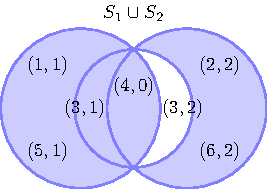
\includegraphics{fig_model_venn.pdf}
  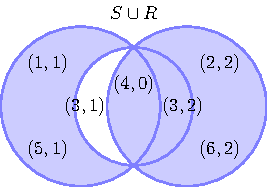
\includegraphics{fig_model_venn_reverse.pdf}
  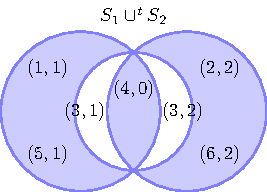
\includegraphics{fig_model_venn2.pdf}
  \caption{Venn diagrams for set and temporal set union operations of
    \acro{TSMS}}
  \label{fig:model:venn}
\end{figure}


\begin{example}\label{ex:model:s1s2}
  Let $R=\{(1,1), (3,1), (4,0), (5,1)\}$ and $S=\{(2,2), (3,2), (4,0),
  (6,2)\}$ be two time series. The union of $R$ and $S$ is $R\cup
  S=\{(1,1), (2,2), (3,1), (4,0), (5,1), (6,2)\}$. Because union is
  not symmetric, $S\cup R=\{(1,1), (2,2), \allowbreak(3,2), (4, 0), (5,1),
  (6,2)\}$. The temporal union results in $R\cupt S= S \cupt
  R=\{(1,1), (2,2), (4,0), (5,1), (6,2)\}$.  
  %
  Venn diagrams for all three cases are shown in
  Figure~\ref{fig:model:venn}, where the coloured area depicts the
  result time series. In every diagram, the central intersection area
  contains measures that share both time and value attributes, like
  instance $(4,0)$. The central left area contains the measures in $R$
  that only share the time attribute with a measure in $S$, like
  instance $(3,1)$. The central right area has a symmetrical
  meaning. The left and right outer areas are the remaining measures
  of $R$ and $S$ respectively.
\end{example}




Time series \emph{difference} can also be defined. Like union, the
difference requires both time series to have the same domain.
%
Let $R$ and $S$ be two time series and let $\dom R = \dom S$.
%
The \emph{difference} between $R$ and $S$, written $R-S$, is a time
series $R-S=\{m|m\in R\wedge m\notin S\}$.
%
The \emph{temporal difference} between $R$ and $S$, denoted $R-^t S$, 
is a time series $R-^t S=\{m|m\in R\wedge m \notinst S\}$.


Based on union and difference we can define \emph{intersection} as
$R\cap S = R - (R - S)$ and \emph{symmetric difference}
as $R \ominus S = (R - S) \cup (S - R)$. The
corresponding temporal operations can also be defined.


Relational \acro{DBMS} extend the set operators by some more such as
selection, rename or join. This kind of operators also make sense for
time series. To illustrate this possibility we define the join
operator.

Roughly speaking, the join of two time series is the combination of
measures sharing the same time attribute.  Let $R$ and $S$ be two time
series.  The \emph{join} of $R$ and $S$, denoted $R \join S$, is a
multivalued time series $R \join S = \{ (t,v_1,v_2) | (t,v_1) \in
R\wedge (t,v_2) \in S\}$. Note that $\dom(R\join
S)=\dom R\times\dom S$.
%
It must be noted that join requires both time series measures to share
exactly the same times. When time series diverge, the temporal
function operations explained later can be applied to adjust the time
instants to join requirements.


A \acro{DBMS} requires computational operators to provide opportunity
to calculate using the data contained. Relational \acro{DBMS} supply
operators like extend, aggregate or
summarise~\cite{date:introduction}. For time series, we define the more
general computational operators \emph{map} and \emph{fold}.

The map operator transforms a time series $S$ into a new time series
$R$ by applying a function to every measure.  Let $S$ and $R$ be two
time series, let $\cal{V}=\dom S$ and $\cal{V'}=\dom R$, and let
$f:\cal{T}\times\cal{V}\rightarrow\cal{T}\times\cal{V'}$ be a function
over a measure returning a measure. The \emph{map} of $f$ over $S$ is
a new time series defined as $\map(S,f)=\{f(m)|m\in S\}$. Note that
$\dom(\map(S,f))=\cal{V'}$.
%


The fold operator recursively combines every measure of a time
series. Assuming that $\mathcal{P}(C)$ is the powerset of $C$, we
define fold as follows.
%
Let $S=\{m_0,\dots, m_k\}$ and $R$ be two time series, let
$\mathcal{V}=\dom S$, let $\mathcal{V'}=\dom R$ and let 
%
$f:\mathcal{P}(\mathcal{T}\times\mathcal{V'}) \times (\mathcal{T}\times\mathcal{V}) \rightarrow \mathcal{P}(\mathcal{T}\times\mathcal{V'})$ 
%
be a function over a time series and a measure, which returns a time
series.
%
The \emph{fold} of $S$ by $f$ with initial value $R$ is a new time
series defined as $\fold(S,R,f) = f(\cdots(f(f(f(R,m_0),\allowbreak
m_1),\allowbreak m_2)\cdots),\allowbreak m_k)$.
%



The classical aggregation operator combines the data of a time series
into a single value.  It is worth to note that it is a special
case of fold.

Let $S=\{m_0,\dots,m_k\}$ be a time series, let $\mathcal{V}=\dom S$,
let $m$ be a measure with $\dom m=\mathcal{V}$, and let 
%
$f:(\mathcal{T}\times\mathcal{V})\times(\mathcal{T}\times\mathcal{V})\rightarrow \mathcal{T}\times\mathcal{V}$ 
%
be a function over two measures returning a measure. The
\emph{aggregate} of $S$ by $f$ with initial value $m$ is a new time
series defined as $\agg(S,m,f) = f(\cdots(f(f(f(m,m_0),\allowbreak
m_1),\allowbreak m_2)\cdots),\allowbreak m_k)$.  

% In the previous fold, the measures are computed in random order.
% However in some computational operations it is necessary to define the
% order, especially when $f$ is not commutative.  Then, it is possible
% to define a \emph{fold with order} as an extension of fold where
% measures are computed in a predetermined order.

% We define a
% \emph{fold with order}, $\orderfold$, as an extension of fold with a
% function $o$ that selects measures in order where $o: S_a \mapsto m_r$
% \[
%  \orderfold(S,S_i,f^f,o) =
%   \begin{cases}
%     S_i  \text{ if } |S|=0, \\
%     \orderfold(S_o,f^f(S_i,m_o),f^f,o)  \text{ else}
%   \end{cases}
% \]
% where $m_o = o(S)$ and $S_o = S - \{m_o\}$.



\begin{example}
\label{ex:computational-operators}
Let $S=\{(1,1),(2,3),(4,1)\}$ be a time series.  Map operator allows
computing a new time series whose values result from time multiplied
by value.  We define the map function $f(t,v)=(t,t\cdot v)$. Then
$\map(S,f)=\{(1,1),(2,6),(4,4)\}$.  
%


The aggregate operator allows, for instance, to compute the measure
that results from the sum of all the values.  To illustrate it, we
define the aggregate function $f(m,n)=(0,V(m)+V(n))$. Now,
$\agg(S,(0,0),f) = (0,5)$, where $5$ is the sum of all the values of
$S$. Note that time is meaningless in this computation.

The fold operator allows, for instance, to select the measures having
its value equal to one.  We define the fold function $f(R,m)=R\cup R'$
where $R'=\{m\}$ if $V(m)=1$ or $R'=\emptyset$ otherwise. Let $m$ be
any measure, note that $f(\emptyset,m)= R'$. Then
$\fold(S,\emptyset,f)=\{(1,1),(4,1)\}$.
\end{example}

%%%%%%% BINARY COMPUTATIONAL OPERATORS

Finally we describe how, using the operators defined before, we can
implement \emph{binary computational} operators between two time
series. This illustrates the power of the operators defined so far.
%

The strategy requires first to join the two time series and then
apply the computational operations. 
%
Let $S$ and $R$ be two time series and $\odot$ be a binary operator on
the value domain. The operator $\odot$ can be extended to the time
series as:
%
$S\odot R=\map(S\join R, f)$ being $f$ the function
$f(t,v,w)=(t,v\odot w)$.
%
This allows to extend real binary operations such as sum, $R+S$, or
division, $R/S$, to time series.


\subsubsection{Sequence operations}
\label{sec:sequence}

Sequence operations manipulate time series considering measures as
being totally ordered by time.  We define three basic operations:
\emph{slice}, \emph{successor} and \emph{concatenation}.


The classical interval concept can be applied to time domain. In this
context, given two time instants $s$ and $t$, we use the notation
$[s:t]$, $(s:t)$, $[s:t)$ and $(s:t]$ respectively for the closed
interval, open interval, open right and open left interval.
%
Following~\cite{last:hetland}, to slice a time series $S$ means to
extract a new time series $R\subseteq S$ constrained to a given time
interval. We denote this operation as the original time series followed
by the interval. Therefore, $S[s:t]=\{m|m\in S \wedge
T(m)\in[s:t]\}$. We can use other intervals to slice a time series in
a same fashion. For instance, $S(s:t]=\{m|m\in S \wedge
T(m)\in(s:t]\}$.

The ordinary time order allows to define the concepts of successor and
predecessor for the measures of a time series.
%
Let $S=\{m_0,\ldots,m_k\}$ be a time series and $m$ be an arbitrary
measure.
%
We say that $m_i=\nex_S(m)$ is the \emph{next} measure to $m$ in $S$ if and
only if $m_i=\inf(S(T(m):+\infty])$.  
%
We also say that $m_i=\prev_S(m)$ is the \emph{previous} measure to
$m$ in $S$ if and only if $m_i=\sup(S[-\infty:T(m)))$. 
%
Infinite measures are obtained when next and previous are applied to
supremum and infimum measures respectively: $\nex_S(\sup
S)=(+\infty,\infty)$ and $\prev_S(\inf S)=(-\infty,\infty)$.

To concatenate two time series means to compute a new time series with
the measures of the first time series followed in time order by the
measures of the second one. 
%
The concatenation requires both time series to share the same domain.
Let $R$ and $S$ be two time series and let $\dom R=\dom S$. The
\emph{concatenation} of $R$ and $S$, denoted as $R||S$, is a time
series that contains all the measures of $R$ together with those of
$S$ that do not intersect with the time interval of $R$. That is,
$R||S= R\cup (S - S[T(\inf R):T(\sup R)])$.



\subsubsection{Temporal function operations}
\label{sec:model:tfunc}

A time series can be thought as discrete representation of an
(original) temporal function. In this section we devise some
operations that manage the time series according to this temporal
function standpoint.  
%

The graph of a function allows to obtain and interpret the
continuous nature of a time series, when the domain of time and value
attributes can be plotted then the graph is equivalent to a graphical
representation.  
%
Let $S$ be a time series and $\cal{T}$ the time domain. The \emph{graph} of
the time series $S$ is a set of ordered pairs $\graph S
=\{(t,S(t))|t\in \cal{T}\}$ where $S(t)$ is a \emph{temporal representation
function} for the time series.
%


Given a time series $S$, the \emph{temporal representation function}
$S(t)$ is a function along the variable $t$ in the domain of
time and the target in the domain of values.
%
In some sense, $S(t)$ can be thought as the original temporal function
from which $S$ was obtained.
%

There is not an unique way to obtain $S(t)$ for a given time series
$S$. Because of this, in temporal representation functions we will
introduce a superscript, say $r$, that shows the name $r$ of the
representation method used. Then, $S(t)^r$ means the representation
function of $S$ using method $r$. Below, we exemplify the
representation functions using two different methods based on impulse
and constant piecewise functions.


\begin{definition}[Dirac representation] 
  Dirac delta (\dd) is a method of representation based on the Dirac
  delta function. Let $S$ be a time series. We define $S(t)^\dd$ as
  the following \dd{} representation function:
  \[
  S(t)^\dd
  =  \begin{cases}
          V(m) & \text{if } \exists m\in S:t=T(m) \\
          0    & \text{otherwise}
  \end{cases}
  \]
\end{definition}

\begin{definition}[Zohe representation]
  Zero-order hold everted (\zohe{}) is a method of representation
  based on the \emph{zero-order hold} signal reconstruction method. It
  is a piecewise constant function built from left-continuous step
  functions.  Let $S$ be a time series. We define $S(t)^\zohe$ as the
  following representation function:
  \[
  S(t)^\zohe 
  = \begin{cases}
    V(m) & \text{if } \exists m\in S: t\in \big(T(\prev_S(m)):T(m)\big]\\
    0    & \text{if } t > T(\max(S)) 
  \end{cases}
  \]
\end{definition}




The concept of representation is used for formalising some set and
sequence operators as temporal operators. 

% Consequently, the result of each one will depend on a representation
% method, which is indicated as a parameter.


We define a temporal interval operation to introduce this concept.
Let $S$ be a time series, let $[s:t]$ be an interval of two time
instants and let $r$ be a representation method. The \emph{temporal
  interval}, denoted as $S[s:t]^r$, returns a new time series with
measures in the interval temporal range. That is, $S[s:t]^r = S(u)^r$
for all $u \in [s:t]$. This is a general definition difficult to
implement, so for every representation a particular temporal interval
must be interpreted:

\begin{itemize}
\item Let $S(t)^\dd$ be the \dd{} representation for $S$. The
  \emph{\dd{} temporal interval} is $S[s:t]^\dd = S[s:t]
  \cup \{m\} \cup \{n\}$ where $m=(s,0)$ and $n=(t,0)$.

\item Let $S(t)^\zohe{}$ be the \zohe{} representation for $S$. The
  \emph{\zohe{} temporal interval} is $S[s:t]^\zohe{} = S(s:t]
  \cup \{m\}$ where $m=(t,v)$ and $v= V(\inf( S[t:+\infty] ))$.
\end{itemize}



From temporal interval other operators can be defined such as temporal
selection, temporal concatenation, or temporal join. As example the
definition of temporal interval operation is given.


The temporal selection over a time series allows to change the
resolution in the context of a representation function.  Let $S$ be a
time series, let $T=\{t_0,t_1,\dotsc,t_k\}$ be a set of time instants, and let 
$r$ be a representation method. The \emph{temporal selection}, denoted as
$S[T]^r$, is a time series with measures in $T$ times computed in
coherence with the representation method $r$. That is, $S[T]^r = S[t_0:t_0]^r
\cup S[t_1:t_1]^r \cup \dotsb \cup S[t_k:t_k]^r$. Let $t$ be a time
instant, note that temporal selection depends on the temporal interval
operation $S[t:t]^r$, which is equivalent to the notion of
temporal representation function over a single time instant. That is, $S[t:t]^r
= \{ (t, S(t)^r) \}$.




The temporal selection operation also allows to regularise a irregular
time series. Let $S$ be a time series, let $d,e\in\cal{T}$ be the
desired regularity parameters, and let $k\in\N$ be a limit for the
scope of the range.  A regularised $S$ can be obtained with $S[T]^r$
where $T = \{e+nd | n\in\N \wedge n\leq k \}$ is a set of time
instants equi-spaced.






\section{Multiresolution model}
\label{sec:MTSMS}

In this section we formalise a model for \acro{MTSMS}. Illustration
examples of the definitions given can be found at the end of the
section. Furthermore, in Section~\ref{sec:features} we have
intuitively introduced the concept of multiresolution through an
example.

A \acro{MTSMS} is a \acro{TSMS} that stores time series using a lossy
compression approach. 
%
The \acro{MTSMS} model is based on the concepts of \emph{measures} and
\emph{time series} as defined in Section~\ref{sec:model:TSMS}. We call
\emph{multiresolution time series} to each time series stored in a
\acro{MTSDB}.
%
A multiresolution time series is a collection of \emph{resolution
  subseries} that store a view of the original time series in a given
resolution.
%
The operator that adds data to a resolution subseries requires to
temporarily accumulate measures in a \emph{buffer}. This allow to
aggregate original data to obtain the expected resolution and finally
store them in a \emph{disc}.


\begin{figure}
  \centering
  %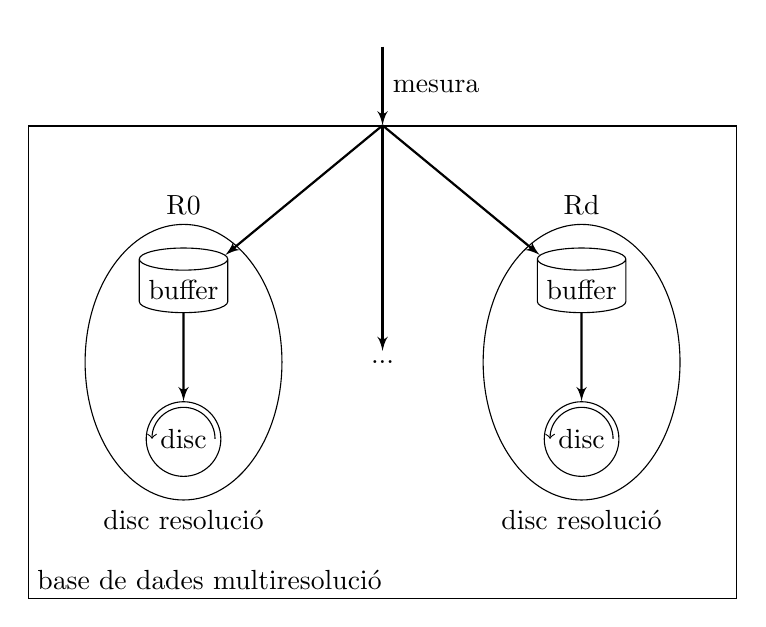
\begin{tikzpicture}
 \tikzset{
        myarrow/.style={->, >=latex',  thick},
      }
      

  \node[rectangle,draw,minimum height=6cm,minimum width=9cm] (m) {};
  \draw[shift=( m.south west)]   
  node[above right] {base de dades multiresolució};


  %discmig
  \node (m.center) (discr1) {...};

  %discr
  
  \node[ellipse,draw,minimum height=3.5cm,minimum width=2.5cm,alias=discr0] [left=of discr1] {};
  \node[above=0cm of discr0.north] {R0};
  \node[below=0cm of discr0] {disc resolució};

  \node[cylinder, draw, shape border rotate=90, aspect=0.25,alias=buffer0] [below=3mm of discr0.north] {buffer};
  \node[circle, draw,alias=disc0]  [above=3mm of discr0.south] {disc} ;
  \draw [->] (disc0.center)++(.4:.4cm) arc(0:180:.4cm);
  \draw[myarrow] (buffer0.bottom) -- (disc0.north);


  %discrd

  \node[ellipse,draw,minimum height=3.5cm,minimum width=2.5cm,alias=discrd] [right=of discr1] {};
  \node[above=0cm of discrd] {Rd};
  \node[below=0cm of discrd] {disc resolució};

  \node[cylinder, draw, shape border rotate=90, aspect=0.25,alias=bufferd] [below=3mm of discrd.north] {buffer};
  \node[circle, draw,alias=discd]  [above=3mm of discrd.south] {disc} ;
  \draw [->] (discd.center)++(.4:.4cm) arc(0:180:.4cm);
  \draw[myarrow] (bufferd.bottom) -- (discd.north);



  %mesura 
  \node[above=1cm of m.north] (m0) {};

  \draw[myarrow] (m0) -- (m.north) 
  node[right,midway] {mesura};

  \draw[myarrow] (m.north) -- (buffer0);
  \draw[myarrow] (m.north) -- (bufferd);
  \draw[myarrow] (m.north) -- (discr1);

\end{tikzpicture}
  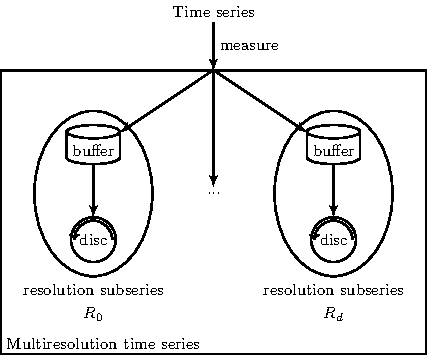
\includegraphics{fig_model_mtsdb.pdf}
  \caption{Architecture of \acro{MTSMS} model}
  \label{fig:model:mtsdb}
\end{figure}

Figure~\ref{fig:model:mtsdb} shows the architecture of a
\acro{MTSMS} for a single multiresolution time series.
%
In this way, the original time series gets stored in the resolution
subseries, each with a different time resolution and distinct
attribute aggregation policies. Discs are size bounded so they only
contain a fixed amount of measures. When a disc becomes full it
discards a measure. Thus, a multiresolution database is bounded in
size and the time series gets stored in a number of storage bounded
time subseries.

Regarding operations, the \acro{MTSMS} model requires two kind of
operators. Some operators should be devoted to set up the time
intervals between measures and to aggregate the attributes. Some other
operators should be dedicated to query the multiresolution schema and
to extract the time series data.

Following, we define the \acro{MTSMS} model structure and the
structural operators, the operations to query a multiresolution
schema, and the \emph{attribute aggregate functions}.  Although schema
manipulation operations could be defined, in this paper we exclusively
focus on structure and data query operators.


\subsection{Structure}

A \emph{buffer} is a container for a time series. The aim of the
buffer is to regularise the time series using a constant
\emph{resolution step} and an \emph{attribute aggregate function}.  We
name \emph{consolidation} to this action of regularisation.  Note that
the attribute aggregate functions are defined in
Section~\ref{sec:model:interpolador}.

\begin{definition}[Buffer]
  Let $S$ be a time series, let $\tau\in\cal{T}$ be the last
  consolidation time, let $\delta\in\cal{T}$ be the resolution step
  and let $f$ be an attribute aggregate function. We define a
  \emph{buffer} $B$ as the tuple $B=(S,\tau,\delta,f)$.
\end{definition}

An empty buffer is noted as $(\emptyset, t_0, \delta, f)$, that is an
empty time series, an initial consolidation time $t_0\in\cal{T}$, a
resolution step $\delta$ and a function $f$.  Given a buffer all the
consolidation time instants can be determined as $\tau_n=t_0+n\delta$
for all $n\in\N$.

Let $B=(S, \tau, \delta, f)$ be a buffer. The \emph{consolidation} of
$B$ is an operation that computes a new measure $m=f(S, \tau, \delta)$
summarising the data of $S$ comprised in the given interval.

A buffer has two main structural operations. The first one adds a
measure to the buffer and the second one consolidates the buffer.

Let $B=(S,\tau,\delta,f)$ be a buffer and let $m$ be a measure.  The
addition of $m$ to $B$, noted as $\addB(B,m)$, returns a new buffer
$\addB(B,m)=(S',\tau,\delta,f)$ where $S' = S \cup \{m\}$.

Let $B=(S,\tau,\delta,f)$ be a buffer. The consolidation of $B$, noted
as $\consB(B)$, returns a new buffer and a new measure $\consB(B)=(B',m')$
where $ B'= (S[\tau+\delta:+\infty], \tau+\delta,\delta,f)$ and $m' =
f(S,\tau,\delta)$. Note that after the consolidation, the
consolidated part of the time series can be removed from the buffer:
historic data is discarded.

The consolidation of a buffer is applied to the first non consolidated
time instant and the total consolidation is obtained by successive
application of the operator. 
%
This requires measures to be added by time order and to consolidate
the buffer when the time of some measure is bigger than the buffer's
next consolidation time.  
%
Let $B=(S,\tau,\delta,f)$ be a buffer and $m=\sup S$ the maximum
measure of $B$. We say that $B$ is consolidable if and only if $T(m)
\geq \tau+\delta$.

A \emph{disc} is a finite capacity container of measures. A time
series stored in a disc has its cardinal bounded. When the cardinal of
the time series is to overcome the limit, some measures need to be
discarded.

\begin{definition}[Disc]
  Let $k\in\N$ and $S$, $|S|\leq k$, be a time series. We define a
  \emph{disc} $D$ as the tuple $D=(S,k)$.
\end{definition}

An empty disc is noted as $(\emptyset,k)$. It is the tuple of an
empty time series and a bound $k$.

The main operation on a disc is to add a measure while keeping under
control the cardinal of the times series. Let $D=(S,k)$ be a disc and
let $m$ be a measure.  The addition of $m$ to $D$, written as
$\addD(D,m)$, is a new disc $\addD(D,m)=(S',k)$ where
%
\[
S' = \begin{cases}
  S\cup\{m\}                 & \text{if } |S|<k  \\
  (S-\{\min S\}) \cup \{m\} & \text{otherwise}
\end{cases}  
\]

A \emph{resolution subseries} is a structure that regularises and
aggregates a time series. It is composed of a buffer, which contains
the time series to be regularised, and a disc, which contains
the regularised time series.


\begin{definition}[Resolution subseries]
  Let $B$ be a buffer and let $D$ be a disc.  We define a
  \emph{resolution subseries} $R$ as the tuple $R=(B,D)$.  
\end{definition}
 
The operators of a resolution subseries extend the buffer and disc
ones. Let $R=(B,D)$ be a resolution subseries and let $m$ be new a
measure.  The addition of $m$ to $R$, noted as $\addR(R,m)$, is a new
resolution subseries $\addR(R,m)=(B',D)$ where $B'= \addB(B,m)$ is the
addition of the measure to the buffer.  The consolidation of $R$,
noted as $\consR(R)$, is a new resolution subseries
$\consR(R)=(B',D')$ where $(B',m') = \consB(B)$ is the consolidation
of the buffer and $D'= \addD(D,m')$ is the addition of the
consolidated measure to the disc. A resolution subseries is
consolidable only when its buffer is consolidable.

A \emph{multiresolution time series} is a set of resolution subseries
referred to the same time series. We store a time series regularised
with distinct resolutions across the resolution subseries, as
previously shown in Figure~\ref{fig:model:mtsdb}.

\begin{definition}[Multiresolution time series]
  Let $M=\{R_0, \dots, R_k\}$ be a finite set of resolution
  subseries. Then $M$ is a \emph{multiresolution time series}.
\end{definition}

Therefore, to define a multiresolution time series we must define the
number of resolution subseries and its corresponding parameters
$(\delta,\tau,f,k)$.  Usually there are no repeated pairs of
$(\delta,f)$ parameters among a multiresolution series, so they act as
key attributes.

The operators of a multiresolution time series apply to every
resolution subseries contained. Let $M=\{R_0,\allowbreak
\dots,\allowbreak R_k\}$ be a multiresolution time series and let $m$
be a measure.
%
The addition of a measure to every resolution subseries, noted as
$\addM(M,m)$, is a new multiresolution time series $\addM(M,m)=\{R'_0,
\dots,\allowbreak R'_k\}$ where $R'_i=\addR(R_i,m)$. The consolidation
of all resolution subseries, noted as $\consM(M)$ is a new
multiresolution time series $\consM(M)=\{R'_0,\allowbreak
\dots,\allowbreak R'_k\}$ where
\[R'_i=
\begin{cases}
\consR(R_i) & \text{if } R_i \text{ consolidable}\\
 R_i & \text{otherwise}
\end{cases}
\]

% The multiresolution consolidation operation should be applied
% regularly based on a consolidation clock. When the measure ordered
% addition approach is taken as explained in the buffer's consolidation,
% then there is no need for a clock in a \acro{MTSMS}. The consolidation
% clock is induced by the measure's addition and then it is only
% necessary to check the multiresolution consolidation operation on new
% additions. However, there could be other approaches where the
% consolidation clock was given by an external clock or external
% events. Then the consolidable definitions would depend on this
% external clock.





\subsection{Queries}

There are two basic time series queries for a \acro{MTSMS}: (i) to
extract a time subseries from a resolution subseries or (ii) to query
for a total time series from all consolidated data.

% Aquesta sembla una consulta una mica circumstancial i menor ...
Let $M$ be a multiresolution time series and let $(\delta,f)$ be a
pair of key attributes.  The first query, denoted as
$\seriedisc(M,\delta,f)$, is a time series such that $\exists (B,D)
\in M: B=(S,\tau,\delta,f) \wedge D=(\seriedisc(M,\delta,f), k) $
where $S,\tau,k$ are bound variables.  Note that we
assume there are no repeated $(\delta,f)$ pairs in $M$.

Let $M=\{R_0,\dots,R_k\}$ be a multiresolution time series and let
$S_0,\dots,S_k$ the time series corresponding to the resolution
subseries $R_0,\dots,R_k$. Assume that the attribute aggregation
functions of all $R_i$ are the same and the resolution steps of all
$R_i$ are distinct.
%
We note as $\totalseries(M)$, the time ordered concatenation of all
time subseries. Recall that $R||S$ is the concatenation for two time
series $R$ and $S$, which has been defined in
Section~\ref{sec:sequence}. Assume that $i_0,\dots,i_k$ is a
permutation of $[0,k]$ such that $\delta_{i_0} < \delta_{i_1} < \cdots
< \delta_{i_k}$ being $\delta_i$ the resolution step of the resolution
subseries $R_i$. Then, $\totalseries(M) = S_{i_0} || S_{i_1} || \cdots
|| S_{i_k}$.
%
TotalSeries obtains the better possible resolution.

From these aforementioned basic time series queries, more elaborated
queries can be applied to \acro{MTSMS} by using \acro{TSMS}
operations. For example, let $L$ and $M$ be two multiresolution time
series, we can compute the sum of both as $\totalseries(L) +
\totalseries(M)$. Recall that $R+S$ is the sum of the values of two
time series $R$ and $S$, which has been defined in
Section~\ref{sec:set} as a binary computational operator.


\subsection{Attribute aggregate function}
\label{sec:model:interpolador}

Attribute aggregate functions are a specific case of \acro{TSMS}
aggregate operations used to summarise time series data while
consolidating a buffer.
%
% Let $S$ be a time series and let $[x,v]$ be a
% time interval. An attribute aggregate function $f$ calculates a new
% measure $m=f(S,[x,v])$. Then, this resulting measure $m$ is interpreted to
% summarise the measures of $S$ for the consolidation interval $[x,v]$.

Let $S$ be a time series, let $\delta$ be a resolution step and let
$\tau$ be a consolidation time.  An \emph{attribute aggregate function} $f$
calculates a new measure $m=f(S,\tau,\delta)$. From $\tau$ and
$\delta$, we obtain the time interval $[\tau:\tau+\delta]$.  Then, the
resulting measure $m$ is interpreted to summarise the measures of $S$
for the time interval $[\tau:\tau+\delta]$.



% \[
% f : S=\{m_0,\ldots,m_k\} \times I=[t_i,t_j] \mapsto m'
% \]
% \[
% f: \cal{P}(\cal{T}\times\cal{V}) \times (\cal{T}\times\cal{T}) \rightarrow \cal{T}\times\cal{V}
% \]

An attribute aggregation function follows this general schema. First,
it obtains a time subseries $S'$ according to the consolidating
interval using a slice operator. For example, $S' =
S[\tau:\tau+\delta]$. Second, it applies a \acro{TSMS} aggregation
function on this time subseries to obtain $m$. For instance, $m =
\agg(S',n, f)$, being $f$ an aggregation function and $n$ an initial
measure, as defined in Section~\ref{sec:set}.

Many different attribute aggregate functions can be used in order to
summarise a time series, for example it is possible to calculate an
statistic indicator of the time series such as the average or a more
complex digital signal processing operation as proposed
by~\cite{zhang11}. Furthermore, the representation of a time series
and some of its pathologies can be considered during the aggregation
process.

Given the diversity of attribute aggregate functions, no global
assumptions can be made about them. Each user should decide which
combination of aggregation and representation fits better to the
measured phenomena.  Therefore, the \acro{MTSMS} model must have a
generic design that allows the users to define their own aggregate
functions.

In what follows we will give some examples of usual attribute
aggregation functions. These functions compute a new measure given a
set of known measures. Then, an attribute aggregation function should
compute a new \emph{time} and a new \emph{value} from the set known measures.
%
% For the rest of this Section we will write $m=f(S,[x,v])$ be the
% resulting measure of an attribute aggregation function $f$ applied to
% a time series $S$ for a time interval $[x,v]$.

% Sobre el calcul del nou temps

The attribute aggregation functions generally return measures that
match the buffer consolidating times. Assume, for instance, that $f$
is an attribute aggregation function and let $m=f(S,\tau,\delta)$.
Then, the time of $m$ is usually computed as $T(m)=\tau+\delta$.
%
However, in some cases it is preferred that $T(m)$ do not match the
buffer consolidating times.
%
For instance, the resulting measure can be aggregated from a time
subseries $S'$ using an open interval $S'=S(\tau:\tau+\delta)$, a
closed interval $S'=S[\tau:\tau+\delta]$, or other combinations like
$S'=S(\tau-d:\tau+\delta-d]$, where $d$ is a time duration that delays the
consolidation to $T(m)=\tau+\delta-d$.
%
This time offset can also be variable. For example, an aggregate
function that returns the first measure of the interval
$m=\min(S[\tau:\tau+\delta))$, then the resulting time fulfils that
$\tau\leq T(m) < \tau+\delta$.

% Sobre el calcul del nou valor
Assume that $f$ is an attribute aggregation function and let
$m=f(S,\tau,\delta)$.  An attribute aggregation function $f$ should
compute the value of $m$.
%
Next there are some examples that illustrate how to compute $V(m)$
based on the temporal function time series operators. 
That is, the time series aggregated is interpreted by the temporal
representation function $S(t)^r$ as has been described in
Section~\ref{sec:model:tfunc}. 
%
In these example functions we leave the time series representation $r$
uninstantiated.

\begin{itemize}
\item The \emph{maximum} computes $V(m)$ as $V(m) =
  \max\limits_{\forall t \in [\tau:\tau+\delta]} S(t)^r$. It
  summarises $S$ with the maximum of the measure values in the
  interval $[\tau:\tau+\delta]$.
\item The \emph{last} computes $V(m)$ as $V(m) = S(\tau+\delta)^r$. It
  summarises $S$ with the value at $\tau+\delta$ time instant.
\item The \emph{mean} computes $V(m)$ as $V(m) = \frac{1}{\delta}
  \int\limits_{\tau}^{\tau+\delta} S(t)^r dt$. It summarises $S$ with
  the mean of the function in the interval $[\tau:\tau+\delta]$.
\end{itemize}

The time series representation in previous examples can be
instantiated in several ways. In what follows we exemplify this
instantiating $r$ as \dd{} and \zohe{}.

Dirac delta attribute aggregation functions interpret the resulting
time as centered on the interval $T(m)=\frac{2\tau+\delta}{2}$. The
resulting value $V(m)$ depends on the attribute, let
$S'=S[\tau:\tau+\delta]^\dd$ be the selection of measures by Dirac
delta temporal interval. Then,
\begin{itemize}
\item The $maximum^\dd$ is such that $V(m) =
  \max\big(0,\max\limits_{\forall n \in S'} V(n)\big)$.
\item The $last^\dd$ is such that $V(m) = V(\max S')$.
\item The $mean^\dd$ is such that $V(m) = \frac{1}{\delta}
  \sum\limits_{\forall n \in S'} V(n)$. Note that for the Dirac
  delta function $\int\dd(t)dt=1$.
\end{itemize}

Note that $\sum\limits_{\forall n \in S'} V(n)$ is a sum of values
that could be implemented as $\agg(S',(0,0),f)$ where
$f(m,n)=(0,V(m)+V(n))$, as shown in
Example~\ref{ex:computational-operators}.

\zohe{} attribute aggregation functions interpret the resulting time
as the right limit of the interval $T(m)=\tau+\delta$. The resulting
value $V(m)$ depends on the attribute, let
$S'=S[\tau:\tau+\delta]^\zohe{}$ be the selection of measures by
\zohe{} temporal interval. Then,

\begin{itemize}
\item The $\maxz$ is such that $V(m) = \max\limits_{\forall n \in S'}
  V(n)$.
\item The $last^\zohe{}$ is such that $V(m) = V(\max S')$.
\item The $\meanz$ is such that $V(m) = \frac{1}{\delta}
  \big[(T(o)-\tau)V(o) + \sum\limits_{\forall n\in R}( T(n)-
  T(\prev_S n) )V(n)\big]$ where $o=\min S'$ and $R= S' - \{o\}$.
\end{itemize}

Note that  $\meanz$ is a sum of values
that could be implemented as $\meanz = \frac{1}{\delta}\agg(S',(0,0),f)$ where $f(m,n)=(0,V(m)+v)$ and 
\[
 v= 
 \begin{cases}
   (T(n)-\tau)V(n) & \text{if } n=\min S'\\
   (T(n)-T(\prev_{S'} n))V(n) & \text{else }
 \end{cases}
\]

\emph{RRDtool}, \cite{rrdtool}, uses an aggregation function similar
to $\meanz$ to summarise velocity counter data by keeping the area
below the original signal.

It is interesting to note that some attribute aggregation patterns are
very similar. For instance, the maximum and last attribute aggregation
schemes differ basically on the interval selection operation. However,
other patterns have a more elaborated interpretation depending on the
actual representation used. This is the case of $\meanz$ and $mean^\dd$.


\begin{example}\label{ex:model:smultiresolution} 
  We define a multiresolution schema for a time series, we consolidate
  the database and we query its data.  Let $S = \{
  (1,6),(5,2),\allowbreak (8,5),\allowbreak (10,0),\allowbreak
  (14,1),\allowbreak (19,6),\allowbreak (22,11),\allowbreak
  (26,6),(29,0) \}$ be a time series and let $M=\{R_0,R_1\}$ be a
  multiresolution time series where each resolution parameters are
  $\tau_0=0$ , $\delta_0=5$, $f_0 =\meanz$, $k_0=4$ and $\tau_1=0$,
  $\delta_1=10$, $f_1 =\maxz$, $k_1=2$. Therefore $R_0$ will be
  consolidated at time instants 5, 10, 15, 20, 25, 30\dots and $R_1$
  at 10, 20, 30\dots

  All measures of $S$ are added to $M$
  and then it is consolidated until it is no more consolidable. As
  $T(\max S)=29$, the last consolidation times are $\tau_0=25$ and
  $\tau_1=20$, so we call $M_{29}$ to the multiresolution time series
  at this state.

  Then, the two time subseries consolidated are obtained by querying
  $\seriedisc(M_{29},5,\allowbreak \meanz)=\{\allowbreak
  (10,3),\allowbreak (15,\allowbreak 2),\allowbreak (20,7),\allowbreak
  (25,8)\}$ and $\seriedisc(M_{29},\allowbreak 10,\allowbreak \maxz)
  =\allowbreak \{ \allowbreak (10,6),\allowbreak (20,11)\}$. Regarding
  buffers, let $S_0$ and $S_1$ be the $M_{29}$ buffer's time series,
  note that $S_0= \{\allowbreak (26,6),\allowbreak (29,0)\allowbreak
  \}$ and $S_1=\{\allowbreak (22,11),\allowbreak (26,6),(29,0)\}$.

  In this particular example,
  $ \totalseries(M_{29}) = \seriedisc(M_{29},\allowbreak 5,\meanz)$ as $R_0$ has
  twice the resolution than $R_1$ and $k_0$ is bigger than $k_1$. 
\end{example}



%%% Local Variables:
%%% TeX-master: "main"
%%% ispell-local-dictionary: "british"
%%% End:

% LocalWords:  genericity multiresolution subseries consolidable

% LocalWords:  pathologies MTSMS TSMS cardinality multivalued infimum
% LocalWords:  multivalues supremum tuple affinely projectively MTSDB
%  LocalWords:  semitemporal piecewise TotalSeries RRDtool



\chapter{Model SGST}
\label{cap:model:sgst}


En aquest capítol es defineix un model per als sistemes de gestió de
bases de dades per a sèries temporals (SGST). Aquest model
s'estructura en base a dos objectes principals, mesures i sèries temporals.
Ambdós tenen un atribut de temps, el qual requereix un tractament
adequat. El model de SGST es dissenya en tres parts.

\begin{itemize}

\item Primer, es defineix el model d'estructura de les dades, és a
  dir, la forma com es descriuen les mesures i les sèries temporals.  

\item Segon, es defineix el model d'operacions sobre les dades, és a
  dir, els operadors bàsics que permeten modelar el comportament i la
  manipulació de les sèries temporals.

\item Tercer, es descriuen propietats de les sèries
  temporals. Les sèries temporals adquireixen propietats
  variades depenent del context on s'apliquin.

\end{itemize}





\section{Model estructural de dades}

Una sèrie temporal és una relació de temps i valors. A cada parella
temps-valor l'anomenem mesura. Així doncs, una sèrie temporal és un
conjunt de mesures. 


En el nostre cas concret, una mesura es correspon amb un valor mesurat
en un instant de temps i una sèrie temporal esdevé una co\l.lecció de
mesures.





\subsection{Temps}
\label{sec:sgst:temps}

El temps és la variable que ens permet ordenar les mesures.  A tal
efecte, si denominem $T$ el domini del temps, els seus membres
presenten una relació d'ordre total. $T$ pot ser tant un conjunt finit
com infinit i normalment serà un conjunt tancat %(compactificat?)
per a poder incloure les mesures indefinides (v.\
\autoref{def:model:mesura_indefinida}) com a límits.

Per tal de facilitar la comprensió, en el document utilitzarem el
conjunt de reals com a conjunt pels temps. Representarem el conjunt
$T$ amb el conjunt estès de nombres reals $\bar{\R{}} \in
\R{} \cup
\{+\infty,-\infty\}$, \parencite{wiki:extendedreal,cantrell:extendedreal},
també anomenat recta real acabada, el qual és un conjunt tancat.

El conjunt estès de nombres reals té dos punts límits corresponents al
valor impropi infinit, aleshores en notació d'interval el conjunt $T$
es pot escriure com $\bar{\R{}} \in [-\infty,+\infty]$. En referència
amb el conjunt dels nombres reals $\R{}$, les relacions d'ordre i
algunes operacions aritmètiques s'estenen al conjunt $\bar{\R{}}$,
\cite{cantrell:extendedreal}.  Algunes expressions esdevenen
indefinides (p.ex.\ $0/0$) i altres depenen del context, com és el cas
de l'expressió indeterminada $0 \times \infty$ que per exemple en la
teoria de la mesura habitualment es defineix com $0 \times \infty =
0$, \cite{wiki:extendedreal}.


El conjunt dels reals és un espai mètric ja que té definida una funció
distància (o mètrica), com per exemple la distància euclidiana. Com a
conseqüència, ens permet distingir entre instants de temps (els
elements del conjunt) i durades (la mètrica). Observant els instants
de temps com a punts en la recta real, les durades com a segments de
la recta real i especificant un instant de temps com a marc de
referència, es pot definir el temps com a sistema de
coordenades \parencite{iep:time-supplement,wiki:coordinate,kopetz11:realtime}. A
continuació definim el temps de manera que puguem ordenar
esdeveniments, mesurar durades d'esdeveniments i establir quan
esdevenen; és una aproximació ingènua sense abastar detalls complicats
del concepte temps \parencite{iep:time}.

\todo{s'hauria de dir que kopetz també en fa una definició similar}



\begin{definition}[Temps]
  \label{def:model:temps}
  Siguin $t^i_i$ i $t^i_j$ dos instants de temps amb el mateix $t^R$
  com a marc de referència, definim la quantitat de temps o la durada
  $t^d$ com un valor $t^d \in\bar{\R{}}$ que mesura la distància en
  unitats de temps entre dos instants de temps $t^d = d(t^i_i,t^i_j)$
  a on $d$ és la mètrica del conjunt $T$. En el cas que els instants
  de temps es defineixin com a reals, $t^i_i , t^i_j \in \bar{\R{}}$,
  aleshores $t^d = t^i_i - t^i_j$.

  Sigui $T$ el domini del temps, definim un instant de temps $I$ com
  un element del conjunt $I \in T$. Així, un instant de temps és
  l'etiqueta d'un punt en la línia temporal. Seguint la definició de
  sistema de coordenades i prenent els nombres reals com a domini del
  temps, sigui $t^{R}$ un instant de temps marc de referència,
  aleshores els instants de temps es defineixen com un valor $t^i
  \in\bar{\R{}}$ que indica la distància de temps amb signe respecte a
  l'instant de temps de referència $t^i= d(t^{R},I)$ a on $d$ és la
  mètrica del conjunt $T$.
\end{definition}

En resum, els instants de temps es poden veure com una seqüència de
valors reals que indiquen esdeveniments amb ordre clarament definit i
entre dos instants de temps sempre hi ha una durada. Expressarem tant
els instants de temps com les durades amb un real que té unitats de
temps. Aquestes unitats són 'segons' en sistema internacional.

% El marc de referència és un instant de temps que permet definir
% unívocament la posició de qualsevol altre instant de temps en un
% sistema de coordenades.



\subsubsection{Estàndards de temps}

Els estàndards de temps especifiquen com s'ha de mesurar el pas del
temps i com s'han d'assenyalar els instants de temps.
\textcite{allen:timescales} recull diferents estàndards de temps
que existeixen, dels quals a continuació comentem els més habituals.

Actualment l'estàndard de temps habitual per mesurar el pas del temps
és el Temps Atòmic Internacional (TAI), del qual se'n deriva un altre
estàndard més conegut que és el Temps Universal Coordinat (UTC).
Ambdós estàndards assenyalen el instants de temps segons el calendari
Gregorià i el calendari julià. Actualment, de forma genèrica s'utilitza
UTC per a sincronitzar rellotges tot i que en el futur es podria
canviar per un nou estàndard, el Temps Internacional (TI), el qual
també es base en el TAI.

El calendari julià utilitza un estàndard de comptar el temps com a
nombre de dies que han passat des d'una data concreta, la qual
s'anomena època. L'època es correspon amb el concepte d'instant de
temps marc de referència de la \autoref{def:model:temps}. Per defecte
l'època se situa a l'inici del Període Julià tot i que també se solen
utilitzar altres dates assenyalades.

Un altre estàndard semblant al julià és l'Hora POSIX o Hora Unix, el
qual compta el nombre de segons des de l'1 de gener de 1970 basant-se
en el les mesures d'UTC. L'Hora Unix és l'estàndard de temps habitual
en els sistemes operatius de la família Unix. No obstant, aquest
estàndard presenta un problema d'ambigüitat a causa que no té no té en
compte els segons addicionals d'UTC.





\subsubsection{Calendari}

Un cas particular del temps és el calendari. Els calendaris són
definicions pel domini temps que consisteixen en noms per als punts de
la línia de temps i regles per establir la durada entre ells per tal
de que el temps tingui certa relació amb la rotació de la Terra. A
l'apartat anterior hem definit el domini temps de manera general
amb el conjunt de reals, els quals exemplifiquen més clarament el
concepte de sistema de coordenades de temps absolut.

\textcite{dreyer94} situen els calendaris i les seves operacions com a
essencials en els SGST. Tanmateix, pot no ser necessari modelar les
dates i regles de calendari en el model de temps. Els calendaris es
poden observar com a noms que fan referència a instants de temps
quantificables, com els de la \autoref{def:model:temps}. Aleshores,
només cal una eina que sigui capaç de convertir els noms de calendari
a instants de temps.

El fet de que un calendari sigui més o menys complicat no afecta al
model de SGST, sols té incidència en les funcions de conversió
d'instant de temps a calendari i viceversa. Tampoc afecta que els
calendaris siguin ambigus (p.ex.\ dos noms per al mateix instant o
instants sense nom) o que continguin propietats impredictibles (p.ex.\
cas dels segons addicionals en UTC) ja que aquests casos es
corresponen amb la bona definició dels sistemes de calendari.

Així doncs, els calendaris en el model de SGST es poden implementar
com una extensió del model de temps. El tipus de dades ordinal de
calendari Gregorià implementat per
\textcite[cap.~16]{date02:_tempor_data_relat_model} pot servir com a
guia per a la implementació dels calendaris en els SGST.




\subsection{Valor}
\label{sec:sgst:valor}

\todo{T: refer tota la secció}

El \gls{terme:SGBDR:valor} és qualsevol element que és d'un
\gls{terme:SGBDR:tipus}; és a dir, un objecte que
pertany a un determinat conjunt de valors i que té associat les
operacions que s'hi poden aplicar. Exemples de tipus de dades són els
enters, els reals, les cadenes de text i les estructures de dades com
vectors, llistes o \glspl{terme:SGBDR:relacio}.  

\todo{Exemplificar més amb tipus que tenen valors i operacions que se'ls poden aplicar}

%\todo{potser citar que el valor es tracta de manera semblant a l'extensió del model objecte-relacional?}

El model de dades dels valors ha d'incloure una dada que defineixi el
valor indefinit. Més endavant a la
definició~\ref{def:model:mesura_valor_indefinit} es detallen les
propietats de les mesures amb valor indefinit. Seguint l'exemple amb
els reals, el valor indefinit es defineix amb el valor impropi infinit
del conjunt dels reals estès
projectivament, \parencite{cantrell:projectivelyextendedreal},
$\R{}^*\in\R{} \cup \{\infty\}$.


En aquest exemple amb reals, el valor és un escalar però fàcilment es
pot estendre el concepte a valors multivaluats ${\R{}^*}^n$ que
representin una co\l.lecció de valors mesurats en el mateix instant de
temps, tal i com fa per exemple \textcite{assfalg08:thesis}.







\subsection{Mesura}\label{sec:model:mesura} 

Una mesura està formada per la parella de temps i valor.

\begin{definition}[Mesura]
  \label{def:model:mesura}
  Definim \emph{mesura} com el tuple $(t,v)$, en el que $v$ és el
  valor de la mesura i $t$ és l'instant de temps en que s'ha pres
  aquesta mesura.
\end{definition}


Donada una mesura $m=(t,v)$ escriurem $V(m)$ per referir-nos a $v$ i
$T(m)$ per referir-nos a $t$.

L'instant de temps de les mesures indueix una relació d'ordre entre
les mesures.
\begin{definition}[Relació d'ordre]\todo{dir-li temporal, perquè sinó després $m\in S$ queda com $m\in^tS$. Arreglar-ho a les definicions de pertinença }
  \label{def:model:mesura-relacio-ordre}
  Sigui $m=(t_m,v_m)$ i $n=(t_n,v_n)$, direm que l'ordre de la mesura
  $m$ és major o igual que $n$, $m\geq n$, si i solament si $t_m\geq
  t_n$.
\end{definition}\todo{també hem de definir l'ordre parcial $m<n$ per la definició de pertinença no temporal?}


En les definicions de temps i valor s'han estès els conjunts amb
valors impropis, concretament s'ha exemplificat amb el conjunt estès
de nombres reals afí $\bar{\R{}} \in \R{} \cup
\{+\infty,-\infty\}$ i amb el projectiu $\R{}^*\in\R{}
\cup\{\infty\}$,
\parencite{cantrell:extendedreal,cantrell:projectivelyextendedreal}. Aquesta
extensió amb l'element impropi infinit ($\infty$) dóna com a resultat
unes mesures impròpies que anomenarem mesura de valor indefinit i
mesura indefinida.\todo{potser s'hauria de dir de no confondre el valor indefinit amb l'absència de valor; és a dir que en una sèrie temporal les mesures que no hi són, són absents (no s'han pres) i les mesures de valor indefinit s'han pres però tenien un valor erroni o desconegut (més a la secció de patologies).} 

\begin{definition}[Mesura de valor indefinit]
  \label{def:model:mesura_valor_indefinit}
  Definim \emph{mesura de valor indefinit} com el tuple $(t,v)$, en el
  que el valor és $v=\infty$ i l'instant de temps és
  $t\in\bar{\R{}}$.
\end{definition}

\begin{definition}[Mesura indefinida]
  \label{def:model:mesura_indefinida}
  Definim \emph{mesura indefinida} com el tuple $(t,v)$, en el que el
  valor és $v\in\R{}^*$ i l'instant de temps és
  $t\in\{+\infty,-\infty\}$.
\end{definition}

Així doncs, donada una mesura $m$, s'anota la mesura de valor
indefinit com $m=(t,\infty)$ i les mesures indefinides com
$m=(+\infty,v)$ per la positiva i $m=(-\infty,v)$ per la negativa, les
quals normalment s'anotaran també amb valor indefinit:
$m=(+\infty,\infty)$ i $m=(-\infty,\infty)$ respectivament.


Les mesures de valor indefinit es podran utilitzar en aquells casos en
els que el valor de la mesura és desconegut. Els valors desconeguts
són aquells valors que no existeixen (es desconeixen, \emph{missing
  data} ) o que s'ignoren (es descarten, \emph{censoring} o
\emph{truncation}). Els valors que no existeixen prenen el valor
desconegut en el moment de la mesura, en canvi els valors descartats
són marcats com a desconeguts després d'un processament de les dades.

Nota: en alguns sistemes es distingeix entre valors infinits
($\infty$) i valors indefinits (NaN, \emph{not a number}),
\cite{wiki:ieee754}. Aquest no és el cas de les definicions de mesures
indefinides presents.







\subsection{Sèrie temporal}
\label{sec:model:serietemporal}

Les sèries temporals són seqüències de mesures ordenades en el temps.
Tradicionalment s'anomenen sèries temporals tot i que alguns autors les anomenen
seqüències temporals, per exemple a \cite{last:hetland}.  Les sèries
temporals són mesures del mateix fenomen i com a conseqüència el tipus
dels valors de les sèries temporals és homogeni.


\begin{definition}[Sèrie temporal]
  \label{def:serie_temporal}
  Una sèrie temporal $S$ és un conjunt de mesures
  $S=\{m_0,\ldots,m_k\}$ sense temps repetits en la qual
  $\forall i,j: i\leq k, j\leq k, i\neq j : T(m_i)\neq T(m_j)$.
\end{definition}

Per ser un conjunt, les sèries temporals tenen mesura de cardinalitat.
\begin{definition}[Cardinal]
  Sigui $S=\{m_0,\ldots,m_k\}$ una sèrie temporal, definim el nombre
  de mesures que conté la sèrie temporal com el cardinal del conjunt
  $|S|=k+1$. Una sèrie temporal sense mesures és la sèrie temporal
  buida $S_\emptyset= \emptyset = \{\}$, és a dir que no té cap element
  $|S_\emptyset|=0$.
\end{definition}



 
\subsubsection{Formes d'una sèrie temporal}

Una sèrie temporal pot tenir formes diferents segons com s'expressi.
A continuació diferenciem entre tres formes possibles d'una sèrie
temporal: canònica, multivaluada i doble.


La forma bàsica d'una sèrie temporal és la de parelles de temps i
valor a la qual anomenem forma canònica.
\begin{definition}[Forma canònica]
  Sigui $S = \{ m_0, m_1 , \dotsc, m_k \}$ una sèrie temporal,
  s'escriu com $S =  \{
  (t_0,v_0), (t_1,v_1), \dotsc, (t_k,v_k)\}$; és
  a dir com a parelles de temps i valor. A aquesta
  forma l'anomenem canònica.
\end{definition}


Les sèries temporals poden mesurar alhora més d'un fenomen quan
aquests comparteixen els instants de temps de mesura. Aquestes sèries
temporals tenen forma de sèrie temporal multivaluada.

\begin{definition}[Sèrie temporal multivaluada]
  Anomenem sèrie temporal multivaluada a una sèrie temporal que té més
  d'un atribut de valors.  Sigui $S = \{ m_0, m_1 , \dotsc, m_k \}$
  una sèrie temporal és multivaluada si cada mesura $m_i$ és un tuple
  $m_i=(t,v_1,v_2,\dotsc,v_n)$ a on $t$ és un instant de temps i
  $v_1$, $v_2$, \dots, $v_n$ són valors. 

  Una sèrie temporal multivaluada es pot escriure en forma canònica de
  parelles $(t,v)$. És a dir, la sèrie temporal multivaluada en
  forma canònica té mesures $m_i$ com a tuples
  $m_i=(t,(v_1,v_2,\dotsc,v_n))$
\end{definition}

La forma canònica s'utilitza per a generalitzar les sèries temporals
multivaluades en les operacions on el valor multivaluat no és
rellevant. En altres operacions, per exemple la selecció o la junció,
el multivalor és rellevant per treballar-hi o perquè el resultat és
una sèrie temporals multivaluada. 



Hi ha una forma no habitual de les sèries temporals que es dóna quan
tenen dos atributs de temps i a la qual anomenem forma doble.

\begin{definition}[Sèrie temporal doble]
  \label{def:sgst:st-doble}
  Anomenem sèrie temporal doble a una sèrie temporal que té dos
  atributs de temps i dos atributs de valors. Sigui $S =\{m_0, \dotsc,
  m_k\}$ una sèrie temporal és doble si cada mesura $m_i$ és un tuple
  $m_i=(t_1,v_1,t_2,v_2)$ a on $t_1$ i $t_2$ són instants de temps i
  $v_1$ i $v_2$ són valors. De la mateixa manera, a aquesta mesura
  $m_i$ l'anomenem mesura doble.  Una sèrie temporal doble no té dues
  parelles de temps repetides $|\{(t_1,t_2) | t_1,t_2\in S\}| = |S|$.
\end{definition}

La sèrie temporal doble prové d'un producte de dues sèries
temporals. Està pensada com a càlcul intermedi d'altres operacions com
per exemple la junció o el mapatge. 
% La seva forma canònica es
% correspondria de manera semblant a l'exemple de la
% \autoref{fig:model:serietemporal:serietemporal}.









\subsubsection{Relació sèrie temporal}

Una sèrie temporal s'expressa com un conjunt i com a tal és
susceptible d'aplicar-hi els conceptes del model relacional dels
SGBD. A continuació, el que s'ha descrit a l'apartat anterior es torna
a expressar seguint el concepte de relació.


Per ser un conjunt de mesures, s'observa una sèrie temporal com una
relació de grau dos a on la capçalera conté els atributs temps i
valor. Ambdós atributs tenen els dominis de temps i valor descrits a
les seccions \ref{def:model:temps} i \ref{sec:sgst:valor}, com per
exemple el tipus de dades 'reals estesos'. Les relacions de sèries
temporals inclou algunes restriccions més que les relacions:

\begin{itemize}
\item Els temps no poden estar repetits: (\emph{key restriction \{t\}})
\item L'atribut de valor ha de contenir el mateix tipus d'objecte i ha
  d'estar associat al mateix fenomen o fenòmens.
\end{itemize}

Els temps no repetits indueixen un ordre temporal a les sèries
temporals. Tot i així, les relacions, per ser conjunts, conserven la
no definció d'un ordre dels elements. En el model relacional no hi ha
ordre ni en les tuples ni en els atributs a diferència de les
relacions matemàtiques que tenen un ordre d'esquerra a
dreta \parencite[sec.\ 5.3]{date:introduction}.


%\subsubsection{Possibles representacions}

A l'apartat anterior s'han descrit diverses formes d'una sèrie
temporal.  A continuació atenem a les possibles representacions com a
relació d'una sèrie temporal segons les formes que tinguin.

% Com a relació seguint el concepte de possibles
% representacions proposat per \textcite[cap.~5]{date:introduction} ?
% i les formes normals de les relacions [Date]?



\begin{definition}[Representació canònica]
  Sigui $S = \{ m_0, m_1 , \dotsc, m_k \}$ una sèrie temporal amb
  domini $\bar{\R{}}$ pels temps i els valors de les mesures,
  representada com a relació s'escriu com $S = ( \{t: \bar{\R{}}, v:
  \bar{\R{}}\}, \{ \{t:t_0,v:v_0\}, \{t:t_1,v:v_1\}, \dotsc,
  \{t:t_k,v:v_k\} \} )$; és a dir com a parella capçalera i conjunt de
  valors certs. A aquesta representació l'anomenem forma canònica.

  Així doncs, sigui $S_{\emptyset} = \{ \}$ una sèrie temporal buida,
  modelada com a relació s'escriu com $S_{\emptyset} = ( \{t:
  \bar{\R{}}, v: \bar{\R{}}\}, \{ \} )$.
\end{definition}


Degut al format esquemàtic de les sèries temporals, en simplifiquem
l'escriptura de la forma canònica com a conjunt de tuples $(t,v)$ a on
$t$ és el temps i $v$ és el valor. Així doncs quan no hi ha dubte
sobre els dominis ni els noms d'atributs, una sèrie temporal es pot
escriure de manera simplificada com a $S = \{ (t_0,v_0), (t_1,v_1),
\dotsc, (t_k,v_k) \}$, la qual es correspon amb la forma canònica de
la sèrie temporal representada com a conjunt.

Tal com s'utilitza en les relacions, les sèries temporals es poden
visualitzar com a taules. La sèrie temporal $S$ i la $S_{\emptyset}$
es visualitzen com a taula a la
\autoref{fig:model:serietemporal:taula}.

\begin{figure}[tp]
  \centering
  \begin{tabular}[c]{|c|c|}
    \multicolumn{2}{c}{$S$} \\ \hline
    $t$  & $v$ \\ \hline
    $t_0$  & $v_0$ \\
    $t_1$  & $v_1$ \\
    $\dots$  & $\dots$ \\ 
    $t_k$  & $v_k$ \\ \hline
  \end{tabular} \qquad
  \begin{tabular}[c]{|c|c|}
    \multicolumn{2}{c}{$S_{\emptyset}$} \\ \hline
    $t$  & $v$ \\ \hline
      &  \\ \hline
  \end{tabular}
  \caption{Visualització com a taula d'una sèrie temporal}
  \label{fig:model:serietemporal:taula}
\end{figure}




\begin{definition}[Representació multivaluada]
  La representació com a relació d'una sèrie temporal multivaluada buida és
  $S_{\emptyset} = ( \{t: \bar{\R{}}, v_1: \bar{\R{}}\,
  v_2: \bar{\R{}}, \dotsc, v_n: \bar{\R{}}\}, \{ \} )$

  Una sèrie temporal multivaluada es pot escriure en forma canònica de
  parelles $(t,v)$. És a dir, la sèrie temporal multivaluada buida en
  representació canònica és $S_{\emptyset} = ( \{t: \bar{\R{}},
  v: V \}, \{ \} )$ a on el domini de l'atribut valor és de tipus
  relació $V = \{ v_1: \bar{\R{}}\, v_2: \bar{\R{}},
  \dotsc, v_n \}$ amb restricció que els valors relació que hi
  pertanyen només poden tenir un tuple $r \in V: |r| = 1$.
\end{definition}

Com ocorre en les relacions, el nom dels atributs d'una sèrie
temporal pot ser decidit per l'usuari. Per exemple una sèrie temporal
multivaluada amb tres atributs amb nom: $S_{\emptyset} = ( \{t:
\bar{\R{}}, \text{temperatura}: \bar{\R{}}\,
\text{consum}: \bar{\R{}}, \text{volum}: \bar{\R{}}\}, \{
\} )$.


Finalment, també representem una sèrie temporal doble en forma de
relació.
\begin{definition}[Representació doble]
  La representació com a relació d'una sèrie temporal doble buida és
  $S_{\emptyset} = ( \{t_1: \bar{\R{}}, v_1: \bar{\R{}}\,
  t_2: \bar{\R{}}, v_2: \bar{\R{}}\}, \{ \} )$.
\end{definition}




\subsection{Exemples}


\begin{example}[Valors reals]
  Sèrie temporal $S_1$ on el temps i els valors pertanyen a
  $\bar{\R{}}$. Conté la mesura de valor 1 en el temps 2, la mesura de
  valor 3 en el temps 2 i la mesura de valor 1 en el temps 6.

En la forma canònica completa s'escriu com $S_1 = ( \{t:
\bar{\R{}}, v: \bar{\R{}}\}, \{ \{t:2,v:1\}, \{t:3,v:3\},
\{t:6,v:1\} \} )$. També es pot escriure de manera simplificada com a
$S_1 = \{ (2,1), (3,3), (6,1) \}$.


La sèrie temporal $S_1$ es visualitza com a taula a la
\autoref{fig:model:serietemporal:real}, a la qual hi afegim una
visualització com diagrama de dispersió amb el temps a l'eix
horitzontal i el valor a l'eix vertical.

\begin{figure}[tp]
  \centering
  \begin{tabular}[c]{|c|c|}
    \multicolumn{2}{c}{$S_1$} \\ \hline
    $t$  & $v$ \\ \hline
    2  & 1 \\
    3  & 3 \\
    6  & 1 \\ \hline
  \end{tabular} \qquad
  \begin{tikzpicture}[baseline=(current bounding box.center)]
    \begin{axis}[
        timeseriesrel,
        title=$S_1$,
        ]
    \addplot[only marks,mark=*,blue] coordinates {
        (2,1)
        (3,3)
        (6,1)
    };
    \end{axis}
   \end{tikzpicture}
  \caption{Taula i gràfic d'una sèrie temporal amb valors reals}
  \label{fig:model:serietemporal:real}
\end{figure}

\end{example}


\begin{example}[Valors caràcters]
  Sèrie temporal $S_2$ on el temps pertany a $\bar{\R{}}$ i els valors
  són caràcters que pertanyen a $C=\{a,b,\dotsc,z,\infty\}$. Conté el
  caràcters $a$, $c$ i $a$ mesurats respectivament en els temps $2$,
  $3$ i $6$.

De manera simplificada s'escriu com $S_2 = \{ (2,a), (3,c), (6,a) \}$.
La sèrie temporal $S_2$ es visualitza com a taula a la
\autoref{fig:model:serietemporal:caracter}, a la qual hi afegim una
visualització com diagrama de dispersió amb el temps a l'eix
horitzontal i el valor a l'eix vertical no continu.

\begin{figure}[tp]
  \centering
  \begin{tabular}[c]{|c|c|}
    \multicolumn{2}{c}{$S_4$} \\ \hline
    $t$  & $v$ \\ \hline
    2  & a \\
    3  & c \\
    6  & a \\ \hline
  \end{tabular} \qquad
  \begin{tikzpicture}[baseline=(current bounding box.center)]
    \begin{axis}[
        timeseriesrel,
        title=$S_4$,
        yticklabels={0,0,a,b,c},
        ]
    \addplot[only marks,mark=*,blue] coordinates {
        (2,1)
        (3,3)
        (6,1)
    };
    \end{axis}
   \end{tikzpicture}
  \caption{Taula i gràfic d'una sèrie temporal amb valors caràcters}
  \label{fig:model:serietemporal:caracter}
\end{figure}

\end{example}



\begin{example}[Sèrie temporal multivaluada]
  Sèrie temporal $S_3$ on el temps pertany a $\bar{\R{}}$ i hi ha tres
  valors on cadascun pertany a $\bar{\R{}}$. En els temps $2$, $3$ i
  $6$ s'ha mesurat a) un atribut \emph{temp} amb valors $1$, $2$ i
  $1$; b) un atribut \emph{cons} amb valors $2$, $1$ i $2$; i c) un
  atribut \emph{vol} amb valors $3$, $0$ i $3$.



En la forma multivaluada s'escriu com %
$S_3 = ( \{t: \bar{\R{}}, \text{ temp}: \bar{\R{}}, \text{
  cons}: \bar{\R{}},\text{ vol}: \bar{\R{}} \}, %
\{%
\{t:2,\text{ temp}:1 , \text{ cons}:2,\text{ vol}:3 \}, %
\{t:3,\text{ temp}:2 , \text{ cons}:1,\text{ vol}:0 \}, %
\{t:6,\text{ temp}:1 , \text{ cons}:2,\text{ vol}:3 \} %
\} )$. També es pot escriure de manera simplificada com a $S_{3} = (
(t,\text{ temp},\text{ cons},\text{ vol}),\{ (2,1,2,3), (3,2,1,0),
(6,1,2,3) \})$.

La forma canònica és una sèrie temporal amb tuples $(t,v)$, és a dir
\begin{align*}
  S^C_{3} &= ( \{t: \bar{\R{}}, v: \{ \text{ temps}:
  \bar{\R{}}, \text{ cons}: \bar{\R{}},\text{ vol}:
  \bar{\R{}},\} \}, \{ \\
  & \{t:2, v: ( \{ \text{ temp}: \bar{\R{}}, \text{ cons}:
  \bar{\R{}},\text{ vol}: \bar{\R{}},\}, \{ \text{ temp}:1
  ,  \text{ cons}:2,\text{ vol}:3 \}\} ), \\
 & \{t:3, v: ( \{ \text{ temp}: \bar{\R{}}, \text{ cons}:
  \bar{\R{}},\text{ vol}: \bar{\R{}},\}, \{ \text{ temp}:2
  ,  \text{ cons}:1,\text{ vol}:0 \}\} ), \\
 & \{t:6, v: ( \{ \text{ temp}: \bar{\R{}}, \text{ cons}:
  \bar{\R{}},\text{ vol}: \bar{\R{}},\}, \{ \text{ temp}:1
  ,  \text{ cons}:2,\text{ vol}:3 \}\} ) \\
  \} )
\end{align*}


La sèrie temporal $S_3$ i la seva forma canònica es visualitzen com a
taula a la \autoref{fig:model:serietemporal:caracter}, a la qual hi
afegim una visualització com diagrama de dispersió amb el temps a
l'eix horitzontal i els valor a l'eix vertical cadascun amb color
diferent.


\begin{figure}[tp]
  \centering
  \begin{tabular}[tp]{|c|c|c|c|}
   \multicolumn{4}{c}{$S_3$} \\ \hline
    $t$  & temp & cons & vol \\ \hline
    2  & 1 & 2 & 3 \\
    3  & 2 & 1 & 0 \\
    6 & 1 & 2 & 3 \\ \hline
  \end{tabular}\qquad
  \begin{tabular}{|c|ccc|}
    \multicolumn{4}{c}{$S_3^c$} \\ \hline
    \multirow{2}{*}{$t$}  & \multicolumn{3}{c|}{$v$} \\ \cline{2-4}
       & temp & cons & vol \\ \hline
    2  & 1 & 2 & 3 \\
    3  & 2 & 1 & 0 \\
    6  & 1 & 2 & 3 \\ \hline
  \end{tabular} 
  \begin{tikzpicture}[baseline=(current bounding box.center)]
    \begin{axis}[
        timeseriesrel,
        title=$S_3$,
        legend columns = 4,
        every axis legend/.append style={
          at={(1,-0.1)},
          anchor=north east,
          draw = none},
        ]
    \addplot[only marks,mark=*,blue] coordinates {
        (2,1)
        (3,2)
        (6,1)
    };
    \addplot[only marks,mark=*,red] coordinates {
        (2,2)
        (3,1)
        (6,2)
    };
    \addplot[only marks,mark=*,green] coordinates {
        (2,3)
        (3,0)
        (6,3)
    };
    \legend{temp,cons,vol}
    \end{axis}
  \end{tikzpicture}
  %El gràfic d'una multivaluada: es poden pintar dos eixos verticals quan les diferències d'escala siguin molt grans.
  \caption{Taula d'una sèrie temporal multivaluada}
  \label{fig:model:serietemporal:multivaluada}
\end{figure}


\end{example}



\begin{example}[Valors vectors]
  Sèrie temporal $S_4$ on el temps pertany a $\bar{\R{}}$ i el valor
  pertany a $\bar{\R{}}^3$; és a dir és un vector representat amb un
  tuple. Conté el valor $(1,2,3)$ en el temps $2$, el valor $(3,4,5)$
  en el temps $4$ i el valor $(1,2,3)$ en el temps $6$.

De manera simplificada s'escriu com $S_4 = \{ (2,(1,2,3)),
(3,(3,4,5)), (6,(1,2,3)) \}$ i es visualitza com a taula i com a
gràfic a la \autoref{fig:model:serietemporal:vector}.

\begin{figure}[tp]
  \centering
  \begin{tabular}{|c|c|}
    \multicolumn{2}{c}{$S_4$} \\ \hline
    $t$  & $v$ \\ \hline
    2  & (1,2,3) \\
    4  & (3,4,5) \\
    6  & (1,2,3) \\ \hline
  \end{tabular} \qquad
  \begin{tikzpicture}[baseline=(current bounding box.center)]
\begin{axis}[
        timeseriesrel,
        nodes near coords,
        title=$S_4$,
        yticklabels={},
        axis y line=none,
        ]
        \addplot+[only marks,mark=none,blue, point meta=explicit symbolic]
        coordinates {
          (2,0)  [\rotatebox{45}{(1,2,3)}]
          (4,0)  [\rotatebox{45}{(3,4,5)}]
          (5,1)  [\mbox{}]
          (6,0) [\rotatebox{45}{(1,2,3)}]
        };
      \end{axis}
    \end{tikzpicture}
    \caption{Taula d'una sèrie temporal amb valors vectors}
  \label{fig:model:serietemporal:vector}
\end{figure}



S'observa que una sèrie temporal amb valors vectors és diferent d'una
sèrie temporal multivaluada. El domini de la primera són vectors i el
de la segona són relacions d'un sol tuple en els que es pot operar
cada atribut per separat. En els vectors de forma general no es poden
operar cada component per separat sinó que formen una unitat
semàntica. Aquesta diferència de significat prové de si es considera
que es mesuren vectors o atributs diferents, el qual s'observa en la
visualització: el gràfic d'un vector és un espai $R^n$ en canvi el
gràfic d'una sèrie temporal multivaluada és un multigràfic, un gràfic
per a cada atribut.

\end{example}


\begin{example}[Valors sèrie temporal]\label{par:model:exemple-relvalues}
  Sèrie temporal $S_5$ on el temps pertany a $\bar{\R{}}$ i el valor
  és una sèrie temporal del mateix format que en l'exemple 1. Conté
  els tuples de $S_1$ com a valors en el temps $1$ i $2$.

De manera simplificada s'escriu com $S_5 = \{ (1,\{ (2,1), (3,3),
(6,1) \}), (2,\{ (2,1),$ $(3,3),$ $(6,1) \}) \}$ i es visualitza com a
taula a la \autoref{fig:model:serietemporal:serietemporal}.


\begin{figure}[tp]
  \centering
  \begin{tabular}{|c|c|}
    \multicolumn{2}{c}{$S_5$} \\ \hline
    $t$  & $v$ \\ \hline
    1 &   
       \begin{tabular}{|c|c|}
         \hline
         $t$  & $v$ \\ \hline
         2  & 1 \\
         3  & 3 \\
         6  & 1 \\ \hline
       \end{tabular} \\ \hline
    2 & 
       \begin{tabular}{|c|c|}
         \hline
         $t$  & $v$ \\ \hline
         2  & 1 \\
         3  & 3 \\
         6  & 1 \\ \hline
       \end{tabular} \\ \hline
  \end{tabular}
  \caption{Taula d'una sèrie temporal amb valors sèrie temporal}
  \label{fig:model:serietemporal:serietemporal}
\end{figure}

S'observa que la capçalera de $S_5$ és $\{t:\bar{\R{}},v:
\{t:\bar{\R{}},v:\bar{\R{}}\}\}$. És a dir, el valor és
una altra relació, com es descriu per \textcite[sec.\
5.3]{date:introduction}, a on el temps i el valor pertanyen a
$\bar{\R{}}$. Per tant, el valor de $S_5$ és de tipus sèrie
temporal amb valors reals. Tot i així, aquest és un valor especial i
si es desplega la relació s'obté una sèrie temporal doble amb
capçalera $\{t^1,t^2,v\}$.

% Cal insistir que \emph{tots} el valors de $S_5$ han de pertànyer al
% mateix domini \parencite[sec.\ 5.4]{date:introduction}, el qual és
% $\{temps:\bar{\R{}},valor:\bar{\R{}}\}$.


\end{example}




















%%% Local Variables:
%%% TeX-master: "main"
%%% End:







% LocalWords:  SGST multivaluada

\section{Model d'operacions}



\begin{verbatim}
VAR timeseries BASE RELATION
    { t RATIONAL, v RATIONAL }  KEY { t } ;

OPERATOR ts.t(m SAME_TYPE_AS  (timeseries)) RETURNS RATIONAL;
return t FROM TUPLE FROM m;
END OPERATOR;

OPERATOR ts.v(m SAME_TYPE_AS  (timeseries)) RETURNS RATIONAL;
return v FROM TUPLE FROM m;
END OPERATOR;
\end{verbatim}




\subsection{Màxim i suprem}


La relació definida a~\ref{def:model:mesura-relacio-ordre} indueix
sobre una sèrie temporal una relació d'ordre total. Com que la sèrie
temporal s'ha considerat finita i sense elements repetits, quan la
sèrie temporal no és buida això comporta l'existència d'un màxim i
d'un mínim.  Si $S$ és una sèrie temporal, $\max(S)$ i $\min(S)$ són
respectivament la mesura màxima i mínima d'$S$.

\begin{definition}[Màxim i mínim]
  Sigui $S=\{m_0,\ldots,m_k\}$ una sèrie temporal i $n\in S$ una
  mesura.  Direm que $n=\max(S)$ és el màxim de la sèrie temporal si i
  només si $\forall m \in S: n \geq m $.  Direm que $n=\min(S)$ és el
  mínim de la sèrie temporal si i només si $\forall m \in S: n \leq
  m$.
\end{definition}

El $\max(S)$ i el $\min(S)$ no estan definits quan la sèrie temporal
és buida: $S= \emptyset$. En
canvi, el suprem i l'ínfim estan definits per qualsevol
sèrie temporal tal com passa amb el conjunt estès de nombres reals,
\cite{cantrell:extendedreal}.  

\begin{definition}[Suprem i ínfim]
  Sigui $S=\{m_0,\ldots,m_k\}$ una sèrie temporal i $n\in S$ una
  mesura.  Direm que $n=\sup(S)$ és el suprem de la sèrie temporal si
  $n=\max(S)$ en cas que el màxim estigui definit o
  $n=(-\infty,\infty)$ en cas contrari.  Direm que $n=\inf(S)$ és
  l'ínfim de la sèrie temporal si $n=\min(S)$ en cas que el mínim
  estigui definit o $n=(+\infty,\infty)$ en cas contrari.
\end{definition}
Quan la sèrie temporal no és buida, per
ser un conjunt finit i d'ordre total, sempre hi ha un i només un màxim
i un mínim i per tant es corresponen amb el suprem i l'ínfim
respectivament.



Tutorial D:
\begin{verbatim}
OPERATOR ts.max(s1 SAME_TYPE_AS  (timeseries)) RETURNS RELATION SAME_HEADING_AS  (timeseries);
return s1 JOIN ( SUMMARIZE s1 {t} PER (s1 {}) ADD (MAX (t) AS t));
END OPERATOR;

OPERATOR ts.sup(s1 SAME_TYPE_AS  (timeseries)) RETURNS RELATION SAME_HEADING_AS  (timeseries);
return ts.max(ts.union(s1,(RELATION { TUPLE {t -1.0/0.0, v 1.0/0.0} })));
END OPERATOR;
\end{verbatim}



Exemple:
\begin{verbatim}
WITH RELATION {
TUPLE { t 2.0, v 3.0 },
TUPLE { t 4.0, v 2.0 },
TUPLE { t 6.0, v 4.0 }
 } AS ts1: 
ts.max(ts1)
\end{verbatim}
\begin{verbatim}
RELATION {
TUPLE { t 1.0, v 2.0 },
TUPLE { t 5.0, v 3.0 },
TUPLE { t 6.0, v 5.0 },
TUPLE { t 1.0/0.0, v 1.0 }  //1.0/0.0 infinit
 } AS ts2: 
ts.max(ts2)
\end{verbatim}
\begin{verbatim}
WITH RELATION {
TUPLE { t 2.0, v 3.0 },
TUPLE { t 4.0, v 2.0 },
TUPLE { t 6.0, v 4.0 }
 } AS ts1: 
ts.sup(ts1)
\end{verbatim}
\begin{verbatim}
WITH RELATION {
TUPLE { t 2.0, v 3.0 },
TUPLE { t 4.0, v 2.0 },
TUPLE { t 6.0, v 4.0 }
 } AS ts1: 
ts.sup(timeseries)
\end{verbatim}



\subsection{Interval}

Atesa la relació d'ordre induïda pel temps en una sèrie temporal
(def.\ \ref{def:model:mesura-relacio-ordre}) és possible definir el
concepte d'interval sobre la seqüència, semblant a com es fa a \cite{last:keogh,last:hetland}.

\begin{definition}[Interval]
  \label{def:model:st-interval}
  Sigui $S=\{m_0, \ldots, m_k\}$ una sèrie temporal. Definirem el subconjunt
  $S(r,t] \subseteq S$ com la sèrie temporal $S(r,t]=\{m\in S
  | r<T(m)\leq t\}$, a on $r$ i $t$ són dos instants de temps.

  També es defineix la subsèrie $S[-\infty,t)\subseteq S$ com la sèrie
  temporal $S[-\infty,t) = \{m\in S | T(\inf(S))\leq T(m) < t\}$.
\end{definition}
S'observa que la subsèrie $S(r,+\infty]\subseteq S$ és
equivalent a la sèrie temporal $S(r,+\infty] \equiv S(r,T(\sup(S))]$ i
anàlogament $S(-\infty,t] \equiv S(T(\inf(S)),t]$. També s'observa que les subsèries $S(t,t]\subseteq S$ i $S[t,t)\subseteq S$ són equivalents a la sèrie temporal buida $S(t,t] \equiv S[t,t) \equiv \emptyset$ ja que per ser els temps d'ordre total $\nexists T(m): t < T(m) \leq t$ o $\nexists T(m): t \leq T(m) < t$, respectivament. 
%Finalment, s'observa que la subsèrie $S(-\infty,+\infty]\subseteq S$ només és equivalent a la sèrie temporal original quan aquesta no conté la mesura indefinida negativa $S(-\infty,+\infty]\equiv S: (-\infty,v)\notin S$


\begin{verbatim}
OPERATOR ts.interval(s1 SAME_TYPE_AS  (timeseries), l RATIONAL, h RATIONAL) RETURNS RELATION SAME_HEADING_AS  (timeseries);
return s1 WHERE t>l AND t<=h;
END OPERATOR;
OPERATOR ts.interval.ni(s1 SAME_TYPE_AS  (timeseries), h RATIONAL) RETURNS RELATION SAME_HEADING_AS  (timeseries);
return s1 WHERE t<h;
END OPERATOR;
\end{verbatim}



\subsection{Successor}


També atenent a la relació d'ordre induïda pel temps en una sèrie temporal, es
defineix el concepte de mesura següent i mesura anterior en una
seqüència.

\begin{definition}[Successor i predecessor]
  Sigui $S=\{m_0, \ldots, m_k\}$ una sèrie temporal i $l\in S$ i $n$ dues
  mesures. Direm que $l$ és el successor de $n$ en $S$ i ho notarem
  com $l=\seg\limits_S(n)$ si i només si $l=\inf(S(T(n),+\infty])$.
  Direm que $l$ és el predecessor de $n$ en $S$ i ho notarem com
  $l=\ant\limits_S(n)$ si i només si $l=\sup(S[-\infty,T(n)))$.

Quan no hi hagi dubte de la sèrie temporal que marca l'ordre, per
exemple quan $n\in S$, podrem escriure $\seg(n)$ i $\ant(n)$.
\end{definition}
S'observa que s'obtenen mesures indefinides en els casos que la
mesura següent o anterior es calcula respectivament per la mesura
suprema o ínfima de la sèrie temporal: $\seg\limits_S(\sup
S)=(+\infty,\infty)$ i $\ant\limits_S(\inf S)=(-\infty,\infty)$.

De la definició anterior es dedueix que donada una sèrie temporal $S$
que no conté mesures indefinides i donada la mesura indefinida
$o=(+\infty,\infty)$, el predecessor de $o$ sempre és el suprem de la
sèrie temporal $\ant\limits_S( (+\infty,\infty) ) = \sup(S): \forall
m\in S: T(m)\in\mathbb{R}$.  % S\equiv S(-\infty,+\infty)
\emph{Demostració: Sigui $S$ una sèrie temporal i $o=(+\infty,\infty)$
  una mesura indefinida, el predecessor de $o$ en $S$ és una mesura
  $l=\ant\limits_S(o)$ que compleix
  $l=\sup(S[-\infty,T(o)))$. Substituint, s'obté que
  $l=\sup(S[-\infty,+\infty))=\sup(S-m):m\in S:T(m)=+\infty \notin
  \mathbb{R}$, i per tant com que $S$ no té mesures indefinides es
  demostra que $l=\sup(S)$.  } De manera semblant es pot demostrar que
$\seg\limits_S( (-\infty,\infty) ) = \inf(S): \forall m\in S:
T(m)\in\mathbb{R}$.





\begin{verbatim}
OPERATOR ts.next( m SAME_TYPE_AS  (timeseries), s1 SAME_TYPE_AS  (timeseries)) RETURNS RELATION SAME_HEADING_AS  (timeseries);
return ts.inf(ts.interval(s1,ts.t(m),1.0/0.0));
END OPERATOR;
OPERATOR ts.prev( m SAME_TYPE_AS  (timeseries), s1 SAME_TYPE_AS  (timeseries)) RETURNS RELATION SAME_HEADING_AS  (timeseries);
return ts.sup(ts.interval.ni(s1,ts.t(m)));
END OPERATOR;
\end{verbatim}





\subsubsection{Unió}

Per tal que l'operació d'unió de conjunts sigui vàlida per les sèries
temporals cal tenir en compte quan dues sèries temporals tenen mesures
en el mateix instant de temps. En cas d'utilitzar l'operació d'unió de
conjunts la sèrie temporal resultant no compliria amb la definició
\ref{def:serie_temporal} ja que contindria mesures amb temps
repetits. Com a conseqüència, es defineix l'operació d'unió per les
sèries temporals.

\begin{definition}[unió]
  Sigui $S_1=\{m_0^1, \dotsc, m_{k_1}^1\}$ i $S_2=\{m_0^2, \dotsc,
  m_{k_2}^2\}$ dues sèries temporals, la unió de les dues sèries
  temporals $S_1 \cup S_2$ és una sèrie temporal $S=\{m_0, \dotsc,
  m_k\}$ que conté totes les mesures de $S_1$ i les mesures de $S_2$
  no repetides: $S_1 \cup S_2 = \{ m \in S_1 \} \cup \{ m^2 =
  (t^2,v^2) \in S_2 | \forall (t^1,v^1)\in S_1 : t^1 \neq t^2
  \}$. 

  Tal com succeeix amb les relacions, per a poder unir dues sèries
  temporals cal que totes dues tinguin la mateixa estructura; és a dir,
  en termes de SGBDR cal que tinguin la mateixa capçalera.
\end{definition}

Propietats de la unió:

\begin{itemize}
\item La dimensió $k$ de la sèrie temporal resultant està fitada a
  $k_1 \leq k \leq k_1 + k_2$. Nota: a la definició, la dimensió $k$ és
  proporcional al cardinal $|S_1\cup S_2| = k+1$.
\item La unió de sèries temporals no és commutativa. En general
  $S_1\cup S_2 \neq S_2\cup S_1$ tot i que sí que es compleix
  l'equivalència respecte al cardinal $|S_1\cup S_2| = |S_2\cup S_1|$.
\end{itemize}



TutorialD:
\begin{verbatim}
OPERATOR ts.union(s1 SAME_TYPE_AS  (timeseries), s2 SAME_TYPE_AS  (timeseries)) RETURNS RELATION SAME_HEADING_AS  (timeseries);
return s1 UNION (s2 JOIN (s2 {t} MINUS s1 {t}));
END OPERATOR;
\end{verbatim}


Exemple:
\begin{verbatim}
WITH RELATION {
TUPLE { t 2.0, v 3.0 },
TUPLE { t 4.0, v 2.0 },
TUPLE { t 6.0, v 4.0 }
 } AS ts1,
RELATION {
TUPLE { t 1.0, v 2.0 },
TUPLE { t 5.0, v 3.0 },
TUPLE { t 6.0, v 5.0 },
TUPLE { t 10.0, v 1.0 }
 } AS ts2: 
ts.union(ts1,ts2)
\end{verbatim}



\subsubsection{Intersecció}

Per tal que l'operació d'intersecció de conjunts sigui vàlida per les sèries
temporals cal tenir en compte quan dues sèries temporals tenen mesures
en el mateix instant de temps.

\begin{definition}[intersecció]
  Sigui $S_1=\{m_0^1, \dotsc, m_{k_1}^1\}$ i $S_2=\{m_0^2, \dotsc,
  m_{k_2}^2\}$ dues sèries temporals, la intersecció de les dues
  sèries temporals $S_1 \cap S_2$ és una sèrie temporal $S=\{m_0,
  \dotsc, m_k\}$ que conté les mesures de $S_1$ repetides a $S_2$:
  $S_1 \cap S_2 = \{ m^1 = (t^1,v^1) \in S_1 | \exists (t^2,v^2)\in
  S_2 : t^1 = t^2\}$.
\end{definition}

TutorialD:
\begin{verbatim}
OPERATOR ts.intersect(s1 SAME_TYPE_AS  (timeseries), s2 SAME_TYPE_AS  (timeseries)) RETURNS RELATION SAME_HEADING_AS  (timeseries);
return s1 JOIN (s1 {t} INTERSECT s2 {t});
END OPERATOR;
\end{verbatim}




\subsubsection{Unió exclusiva}

Unió de dues sèries temporals sense tenir en compte les mesures que
tenen el mateix instant de temps.


\begin{definition}[unió exclusiva]
  Sigui $S_1=\{m_0^1, \dotsc, m_{k_1}^1\}$ i $S_2=\{m_0^2, \dotsc,
  m_{k_2}^2\}$ dues sèries temporals, la unió exclusiva de les dues
  sèries temporals $S_1 \cup^x S_2$ és una sèrie temporal $S=\{m_0,
  \dotsc, m_k\}$ que conté les mesures no repetides de $S_1$ i de
  $S_2$: $S_1 \cup^x S_2 =  ( S_1 \cup S_2 ) - (S_1 \cap S_2)$.
\end{definition}


TutorialD:
\begin{verbatim}
OPERATOR ts.xunion(s1 SAME_TYPE_AS  (timeseries), s2 SAME_TYPE_AS  (timeseries)) RETURNS RELATION SAME_HEADING_AS  (timeseries);
return ts.union(s1,s2) MINUS ts.intersect(s1,s2) ;
END OPERATOR;
\end{verbatim}


Exemple:
\begin{verbatim}
WITH RELATION {
TUPLE { t 2.0, v 3.0 },
TUPLE { t 4.0, v 2.0 },
TUPLE { t 6.0, v 4.0 }
 } AS ts1,
RELATION {
TUPLE { t 1.0, v 2.0 },
TUPLE { t 5.0, v 3.0 },
TUPLE { t 6.0, v 5.0 },
TUPLE { t 10.0, v 1.0 }
 } AS ts2: 
ts.xunion(ts1,ts2)
\end{verbatim}









\subsection{Temporals}

Operacions a on el temps i la representació de la sèrie temporals
juguen un paper important.


\subsubsection{Pertinença temporal}

\begin{definition}[pertinença temporal]
  Sigui $S=\{m_0, \dotsc, m_{k}\}$ una sèrie temporal i $m=(t,v)$ una
  mesura, direm que la mesura pertany temporalment a la sèrie 
  $m\in^t S$ si i només si $\exists m_i=(t_i,v_i)\in S: t_i=t$.
\end{definition}


TutorialD:
\begin{verbatim}
OPERATOR ts.temporal.in(m SAME_TYPE_AS  (timeseries), s SAME_TYPE_AS  (timeseries)) RETURNS BOOLEAN;
return (TUPLE FROM m {t}) IN (s {t});
END OPERATOR;
\end{verbatim}





\subsubsection{Selecció temporal}

Sigui $S$ una sèrie temporal i $i=[t_0,t_f]$ un interval de temps,
per una banda s'ha definit l'interval sobre la seqüència d'una sèrie temporal $S(t_0,t_f]$ (def.~\ref{def:model:st-interval})  i per altra banda s'ha definit la representació contínua $r$ d'una sèrie temporal $S(t)$ \todo{referenciar la definició de repr}.
Per seleccionar un interval temporal cal tenir en compte tant l'interval sobre la seqüència com la representació contínua, Aquesta selecció temporal s'anota com selecció de $S$ en $i$ amb representació $r$ o bé $S[t_o,t_f]^r$. 

\begin{definition}[Selecció temporal de $S$ en $i$ amb representació
  $r$]
  \[
  \text{selecció}: \text{Sèrie temporal} \times \text{interval de
    temps} \times \text{representació} \longrightarrow \text{Sèrie
    temporal}
  \]
  \[
  S = \{m_0 , \ldots , m_k\}  \times i = [t_0,t_f] \times r \longrightarrow S'
  \]
  \[
  \forall  t \in i: S' = S(t)^r 
  \] 
\end{definition}

A continuació s'exemplifica utilitzant la representació \emph{zoh} enrere.


\begin{definition}[Selecció temporal de $S$ en $i$ amb representació
  \emph{zohe}]
  Sigui $S$ una sèrie temporal, $i=[t_0,t_f]$ un interval de temps i
  \emph{zohe} la representació $S(t)$ amb \emph{zero-order-hold} cap
  enrere, es defineix la subsèrie $S[t_0,t_f]^{\text{zohe}}\subseteq
  S$ com la sèrie temporal 
  \[
  S[t_0,t_f]^{\text{zohe}} = S(t_0,t_f] \cup \{m\} : m=(t_f,v):
  \]
  \[
  v=  V(\inf(S-S[-\infty,t_f)))
  \]

  %Atenció S(t_0,t_f] \cup \{m\} no és equivalent a  (S \cup \{m\})(t_0,t_f] ni sabent que m=(t_f,v); comprovar-ho pel cas t_0=t_f
  
  Nota: $S-S[-\infty,t_f)$ seria equivalent a l'interval tancat
  $S[t_f,+\infty]$ si aquest últim estigués definit.
\end{definition}

Propietats de la selecció temporal:

\begin{itemize}
\item Observeu que, sigui $t_a$ un instant de temps, la selecció de $S$ en $[t_a,t_a]$ és equivalent a la representació contínua $S(t_a)$. 
\end{itemize}



TutorialD:
\begin{verbatim}
OPERATOR ts.temporal.select.zohe(s SAME_TYPE_AS  (timeseries), l RATIONAL, h RATIONAL ) RETURNS RELATION SAME_HEADING_AS  (timeseries);
BEGIN;
VAR x RATIONAL init(0.0);
VAR sp PRIVATE SAME_TYPE_AS ( timeseries) KEY { t };
x := ts.v(ts.inf(s MINUS ts.interval.ni(s,h)));
sp := RELATION {
TUPLE {t h, v x}
};
return ts.union(ts.interval(s,l,h),sp);
END;
END OPERATOR;
\end{verbatim}

Exemple:
\begin{verbatim}
WITH RELATION {
TUPLE { t 2.0, v 3.0 },
TUPLE { t 4.0, v 2.0 },
TUPLE { t 6.0, v 4.0 }
 } AS ts1,
RELATION {
TUPLE { t 1.0, v 2.0 },
TUPLE { t 5.0, v 3.0 },
TUPLE { t 6.0, v 5.0 },
TUPLE { t 10.0, v 1.0 }
 } AS ts2:
ts.temporal.select.zohe(ts1,1.0,5.0)
\end{verbatim}
\begin{verbatim}
WITH RELATION {
TUPLE { t 2.0, v 3.0 },
TUPLE { t 4.0, v 2.0 },
TUPLE { t 6.0, v 4.0 }
 } AS ts1,
RELATION {
TUPLE { t 1.0, v 2.0 },
TUPLE { t 5.0, v 3.0 },
TUPLE { t 6.0, v 5.0 },
TUPLE { t 10.0, v 1.0 }
 } AS ts2:
ts.temporal.select.zohe(ts1,-1.0/0.0,-1.0/0.0)
\end{verbatim}




\subsubsection{Selecció de la resolució}

La selecció de la resolució d'una sèrie temporal permet canviar, en el
context d'una representació, la resolució a una de marcada per un
conjunt d'instants de temps. A diferència d'un buffer, la selecció de
resolució no permet aplicar interpoladors ni obliga a que la sèrie
temporal resultant sigui regular.

Sigui $S$ una sèrie temporal, $i= \{t_0,t_1,\dotsc,t_n\}$ un conjunt
d'instants de temps i la representació contínua $r$ de la sèrie
temporal $S(t)$, la selecció de resolució s'anota com resolució de $S$
en $i$ amb representació $r$ o bé $S[i]^r$.

\begin{definition}[Selecció de la resolució de $S$ en $i$ amb representació
  $r$]
  \[
  \text{resolució}: \text{Sèrie temporal} \times \text{instants de
    temps} \times \text{representació} \longrightarrow \text{Sèrie
    temporal}
  \]
  \[
  S = \{m_0 , \ldots , m_k\} \times i = \{t_0,t_1,\dotsc,t_n\} \times r
  \longrightarrow S'
  \]
  \[
  t_0 < t_1 < \dotsb < t_n:
  \]
  \[
  S' = S[t_0,t_0]^r \cup  S[t_1,t_1]^r \cup \dotsb \cup S[t_{n},t_n]^r
  \] 
  % Es podria fer recursiu
  % \[
  % t_f = \sup(i): i_n = i - t_f: t_a = \sup(i_n):
  % S' = \left\{\begin{array}{ll}
  %     \{\} & \text{si } |i| = 0 \\
  %     S[i_n]^r \cup S[t_a,t_f]^r 
  %   \end{array}\right.
  % \] 
\end{definition}



Propietats de la selecció de resolució:
\begin{itemize}
\item El cardinal de la sèrie temporal resultant és el mateix que el del conjunt d'instants de temps $|S[i]^r| = |i|$
\end{itemize}



TutorialD:
\begin{verbatim}

\end{verbatim}



\subsubsection{Unió temporal}

Unió temporal de dues sèries temporals $S_1 \cup^r S_2$. Per la unió temporal les sèries temporals han de tenir la mateixa estructura, tal com s'ha notat per a la unió de sèries temporals.

\begin{definition}[Unió temporal de $S_1$ i $S_2$ amb representació
  $r$]
  \[
  \text{unió}: \text{Sèrie temporal} \times \text{Sèrie temporal}
  \times \text{representació} \longrightarrow \text{Sèrie temporal}
  \]
  \[
  S_1 = \{m_0^1 , \ldots , m_{k1}^1\}  \times S_2 = \{m_0^2 , \ldots , m_{k2}^2\} \times r \longrightarrow S'
  \]
  \[
  t_1=T(\inf S_1), t_2=T(\sup S_1):
  \]
  \[
  S' = S_1 \cup  ( S_2 - S_2[t_1,t_2]^r )
  \] 
\end{definition}



Propietats de la unió temporal:
\begin{itemize}
\item No commutativa
\item Però, $(S_1 \cup^r S_2) \cup (S_2 \cup^r S_1) = S_1 \cup S_2$\todo{és cert?}
\end{itemize}



TutorialD:
\begin{verbatim}

\end{verbatim}




\subsubsection{Fusió temporal}

Fusió (join) de dues sèries temporals $S_1 \text{ fusió } S_2$.


\begin{definition}[Fusió temporal de $S1$ i $S2$ amb representació $r$]
  \[
  \text{fusió}: \text{Sèrie temporal} \times
  \text{Sèrie temporal} \times \text{representació} \longrightarrow
  \text{Sèrie temporal}
  \]
  \[
  S_1 = \{m_0^1 , \ldots , m_{k_1}^1\} \times S_2 = \{m_0^2 , \ldots ,
  m_{k_2}^2\} \times r \longrightarrow S'
  \]
  \[
  t = \{t^1 \, | \, \forall m^1=(t^1,v^1) \in S_1\} \cup \{t^2 | \forall
  m^2=(t^2,v^2) \in S_2\}:
  \]
  \[
  S' = \{m'=(t',v_1',v_2') \, | \, (t',v_1') \in S_1[t]^r \wedge (t',v_2') \in S_2[t]^r \} 
  \]\todo{els valors s'haurien de saber fusionar}
\end{definition}



Propietats de la fusió temporal:
\begin{itemize}
\item $|S'| <= k_1 + k_2$
\end{itemize}





TutorialD:
\begin{verbatim}

\end{verbatim}







\section{Map i fold}

\begin{align*}
  \text{map}:& S \times f \longrightarrow S' = \{\forall m\in S : f(m) \}, \\
             & \text{a on } f: m \mapsto m' 
\end{align*}





\begin{align*}
  \text{fold}: & S=\{m_0,\dotsc,m_k\} \times m_i \times f \longrightarrow m'= \\
               =& f(\dots(f(f(f(m_i,m_0),m_1),m_2)\dots),m_k), \\
               & \text{a on } f: m_a \times m_b \mapsto m'
\end{align*}


Noteu que $\text{fold}(\{\},m_i,f) \mapsto m_i$ 



% \[
% \text{fold}: S \times m_i \times f(m,m_i) \longrightarrow m' =
% \begin{cases}
%   m_i & si |S|=0 \\
%   f_m & altrament
% \end{cases},
% \text{ a on}
% \]
% \[
% f_m=m_a\in S : \text{fold}( S-\{m_a\},f(m_a,m_i),f)
% \]




\begin{align*}
  \text{mapfold}: & S=\{m_0,\dotsc,m_k\} \times S_i \times f \longrightarrow S'= \\
                 =& f(\dots(f(f(f(S_i\times\{m_0\})\times\{m_1\})\times\{m_2\})\dots)\times\{m_k\}), \\
                  & \text{a on } f: \{S_a \times S_b \}\mapsto S'\\
                  & \text{és a dir? } =map( \{S_a \times S_b \},f)
\end{align*}\todo{s'ha de definir l'operació producte $S_1 \times S_2 \rightarrow S*$ S* pq no és totalment una sèrie temporal?}



Propietats d'operacions mapfold:\todo{comprovar}
\begin{itemize}
\item mapfold:$S \times \{\} \times f \mapsto \{\}$ 

\item mapfold:$\{\} \times S_i \times f \mapsto S_i$ 

\item mapfold:$S \times S_i \times
  \map([S_a\times S_b],(t^1,v^1,t^2,v^2)\mapsto(t^1,v^1)) \mapsto S_i$

\item mapfold:$S \times S_i \times \map([S_a\times
  S_b],(t^1,v^1,t^2,v^2)\mapsto(t^2,v^2)) \mapsto S'$ a on $|S'|=1$

\item Totes les fold es poden implementar com a mapfold$(S,\{m_i\},
  \{m_a \times m_b\} \mapsto \{m'\})$

\item Totes les map es poden implementar com a mapfold$(\{(0,0)\},S,
  \{m_a\} \times  \{\} \mapsto \{m'\})$
\end{itemize}



Exemple d'operacions map:
\begin{itemize}
\item $\text{igual}: S \mapsto S'$ a on $S'= \map(S,(t,v)\mapsto(t,v))$
\item $\text{intercanvia}: S \mapsto S'$ a on $S'= \map(S,(t,v)\mapsto(v,t))$
\item $\text{pes}: S \mapsto S'$ a on $S'= \map(S,(t,v)\mapsto(t,t*v))$
\item $\text{tpredecessors}_{v1}: S \mapsto S'$ a on $S'= \map(S,(t,v)
  \mapsto (t,T(\ant_S(m)))$
\end{itemize}

Exemple d'operacions fold:
\begin{itemize}
\item $\text{cardinal}: S \mapsto m'$ a on $m'=
  \fold(S,(0,0),(t^1,v^1)\times(t^2,v^2)\mapsto(t^2,v^2+1)$
\item $\text{sumaV}: S \mapsto m'$ a on $m'=
  \fold(S,(0,0),(t^1,v^1)\times(t^2,v^2)\mapsto(t^1,v^1+v^2))$
\item $\text{sup}: S \times m \mapsto m'$ a on $m'=
  \fold(S,(-\infty,\infty),(t^1,v^1)\times(t^2,v^2)\mapsto [(t^1,v^1)
  \text{ if } t^2 < t^1 \text{ else } (t^2,v^2) ])$
\item $\text{antM}: S \times m \mapsto m'$ a on $m'=
  \fold(S,(-\infty,\infty),(t^1,v^1)\times(t^2,v^2)\mapsto [(t^1,v^1)
  \text{ if } t^2 < t^1 < T(m) \text{ else } (t^2,v^2) ])$
\end{itemize}


Exemple d'operacions mapfold:
\begin{itemize}
\item $\text{tpredecessors}_{v2}: S \mapsto S'$ a on $S'=
  mapfold(S,S^b,[S^1\times S^2]\mapsto f), S^b =
  \map(S,(t,v)\mapsto(t,-\infty)), f=\map([S^1\times
  S^2],(t^1,v^1,t^2,v^2)\mapsto (t^1,v^2) \text{ if } v^1<t^2<t^1
  \text{ else } (t^1,v^1))$
\end{itemize}




TutorialD:
\begin{verbatim}
WITH RELATION {
TUPLE { t 2.0, v 3.0 },
TUPLE { t 4.0, v 2.0 },
TUPLE { t 6.0, v 4.0 }
} AS ts1: 
ts.map(ts1,'t','t*v/2.0')
\end{verbatim}

TutorialD:
\begin{verbatim}
WITH RELATION {
TUPLE { t 2.0, v 3.0 },
TUPLE { t 4.0, v 2.0 },
TUPLE { t 6.0, v 4.0 }
 } AS ts1,
RELATION {
TUPLE { t 0.0, v 0.0}
} AS mi: 
ts.fold(ts1,mi,'t','v+vi')
\end{verbatim}

antM TutorialD:
\begin{verbatim}
WITH RELATION {
TUPLE { t 2.0, v 3.0 },
TUPLE { t 4.0, v 2.0 },
TUPLE { t 6.0, v 4.0 }
 } AS ts1,
RELATION {
TUPLE { t 5.0, v 0.0}
} AS m: 
ts.sup(ts1 WHERE t < ts.t(m))
\end{verbatim}

sup fold TutorialD:
\begin{verbatim}
WITH RELATION {
TUPLE { t 2.0, v 3.0 },
TUPLE { t 4.0, v 2.0 },
TUPLE { t 6.0, v 4.0 }
 } AS ts1,
RELATION {
TUPLE { t -1.0/0.0, v 1.0/0.0}
} AS mi: 
ts.fold(ts1,mi,'max {t,ti}','v FROM TUPLE FROM (RELATION { TUPLE {t t, v v, e True}, TUPLE {t ti, v vi,  e False} } JOIN RELATION { TUPLE {e t > ti}})')
\end{verbatim}

predecessors mapfold TutorialD:
\begin{verbatim}
WITH RELATION {
TUPLE { t 2.0, v 3.0 },
TUPLE { t 4.0, v 2.0 },
TUPLE { t 6.0, v 4.0 }
 } AS ts1,
EXTEND ts1 {t} ADD ( -1.0/0.0 as v)
AS si: 
ts.fold(ts1,si,'t','v FROM TUPLE FROM (RELATION { TUPLE {v ti, e True}, TUPLE {v v,  e False} } JOIN RELATION { TUPLE {e v < ti and ti<t}})')
\end{verbatim}




%%% Local Variables:
%%% TeX-master: "main"
%%% End:







% LocalWords:  SGST

\section{Propietats de les sèries temporals}

En el model de SGST descrit anteriorment, les sèries temporals tenen
una única estructura i uns únics operadors independentment del context
on s'apliquin. De fet aquest és l'objectiu principal de definir-ne
un model lògic. No obstant això, en la seva aplicació les sèries
temporals tenen associat un context, és a dir que els valors prenen un
determinat significat. En aquesta secció avaluem les propietats que
poden prendre les sèries temporals quan es troben en context:
\begin{itemize}
\item Trets semàntics: el significat que tenen en
  el seu àmbit d'aplicació
\item Grafs i representacions: les visualitzacions i interpretacions
  possibles
\item Patologies: els casos problemàtics de les sèries temporals
\end{itemize}




\subsection{Trets semàntics de les sèries temporals}

Una sèrie temporal pot provenir d'àmbits varis i per tant tenir un
significat variat. És el que anomenem trets semàntics de les sèries
temporals.


En el model d'operacions s'ha vist que l'atribut de temps de les
sèries temporals indueix vàries naturaleses en el comportament dels
operadors: com a conjunts, com a seqüències o com a funcions
temporals. Però aquesta distinció de significat és des del punt de
vista de formalització matemàtica per l'estructura de les sèries
temporals.

A continuació distingim el significat de les sèries temporals segons
l'origen; és a dir com s'han adquirit o de quin entorn
provenen. Aquesta distinció és important per a determinar quines
operacions tenen sentit de ser aplicades i quines no a una sèrie
temporal en particular. Així \textcite{segev87:sigmod} anomenen
comportament semàntic (\emph{semantic behavior}) a la varietat de
formes que pot prendre una sèrie temporal segons l'àmbit on
s'apliquen.


\subsubsection{Aparell de mesura}

Un primer tret semàntic de les sèries temporals és deu al mètode
d'adquisició segons l'aparell de mesura. Així una sèrie temporal es
pot classificar segons si s'ha adquirit mostrejant un senyal continu
cada cert període o si prové d'una acumulació o d'un comptatge
d'esdeveniments en un cert període de temps. Aquests són els dos
orígens principals que poden tenir els senyals discrets segons
\textcite[cap.~1]{proakismanolakis96}.  En aquest tret es distingeix
segons l'adquisició en l'eix del temps, també es pot distingir segons
si l'adquisició en l'eix de valors és contínua o discreta però això és
un tret propi dels valors i, com a característica, pertany al domini
dels valors. Aquest procés en l'eix de valors s'anomena quantització
del senyal però sovint, per simplificar, no es té en
compte \parencite{proakismanolakis96}.%S1.4.7



Així doncs segons l'aparell de mesura, classifiquem una sèrie
temporal amb trets de magnitud física o de comptador de magnitud
física. Aquest tret semàntic cal tenir-lo en compte ja que quan
s'adquireix una magnitud es veu el seu estat instantani actual, mentre
que quan s'adquireix un comptador ofereix informació de la seva
variació respecte a l'adquisició anterior.



\begin{figure}[tp]
  \centering
    \begin{tabular}[c]{|c|c|}
    \multicolumn{2}{c}{$S_m$} \\ \hline
    $t$  & $v$ \\ \hline
    0   & 0 \\
    2   & 1 \\
    3   & 1{,}5 \\
    4   & 0 \\
    5   & 2 \\ 
    8   & 2 \\ \hline
  \end{tabular} \qquad
  \begin{tikzpicture}[baseline=(current bounding box.center)]
    \begin{axis}[
        timeseriesrel,
        title=$S_m$,
        ]
    \addplot[blue] coordinates {
        (0,0)
        (2,1)
        (3,1.5)
        (4,0)
        (5,2)
        (8,2)
    };
    %\addlegendentry{Valor absolut}
    \addplot[only marks,mark=*,red] coordinates {
        (0,0)
        (2,1)
        (3,1.5)
        (4,0)
        (5,2)
        (8,2)
    };
    % \addlegendentry{Punts de mesura}
    \end{axis}
  \end{tikzpicture}
 

  \caption{Magnitud física}
  \label{fig:model:magnitud}
\end{figure}

\begin{figure}[tp]
  \centering
    \begin{subfigure}{\textwidth}
    \centering
  \begin{tabular}[c]{|c|c|}
    \multicolumn{2}{c}{$S_a$} \\ \hline
    $t$  & $v$ \\ \hline
    0   & 0 \\
    2   & 1 \\
    4   & 3 \\
    5   & 4 \\
    8   & 10 \\ \hline
  \end{tabular} \qquad
  \begin{tabular}[c]{|c|c|}
    \multicolumn{2}{c}{$S_\Delta$} \\ \hline
    $t$  & $v$ \\ \hline
    0   & 0 \\
    2 & 1 \\
    4 & 2 \\
    5 & 1 \\
    8 & 6 \\ \hline
  \end{tabular} \qquad
  \begin{tabular}[c]{|c|c|}
    \multicolumn{2}{c}{$S_v$} \\ \hline
    $t$  & $v$ \\ \hline
    0   & 0 \\
    2 & 0{,}5 \\
    4 & 1 \\
    5 & 1 \\
    8 & 2 \\ \hline
  \end{tabular}
  \caption{Taules de valors}
  \end{subfigure}

  \begin{subfigure}{0.3\textwidth}
  \begin{tikzpicture}
    \begin{axis}[
        timeseriesrel,
        title=$S_a$,
        ]
    \addplot[blue] coordinates {
        (0,0)
        (2,1)
        (4,3)
        (5,4)
        (8,10)
    };
    %\addlegendentry{Valor absolut}
    \addplot[only marks,mark=*,red] coordinates {
        (0,0)
        (2,1)
        (4,3)
        (5,4)
        (8,10)
    };
    % \addlegendentry{Punts de mesura}
    \end{axis}
  \end{tikzpicture}
  \caption{Valor absolut}
    \label{fig:model:comptador-formes:absolut}
  \end{subfigure}
  \begin{subfigure}{0.3\textwidth}
  \begin{tikzpicture}
    \begin{axis}[
        timeseriesrel,
        title=$S_\Delta$,
        ]
    \addplot[ycomb,blue,mark=-] coordinates {
        (0,0)
        (2,1)
        (4,2)
        (5,1)
        (8,6)
    };
    %\addlegendentry{Increments}
    \addplot[only marks,mark=*,red] coordinates {
        (0,0)
        (2,1)
        (4,2)
        (5,1)
        (8,6)
    };
    %\addlegendentry{Punts de mesura}

    \addplot[gray,dashed] coordinates {
        (0,0)
        (2,1)
        (4,2)
        (5,1)
        (8,6)
    };
    % \addlegendentry{Tendència}

    \end{axis}
  \end{tikzpicture}
  \caption{Increments}
  \label{fig:model:comptador-formes:increments}
  \end{subfigure}
 \begin{subfigure}{0.3\textwidth}
  \centering
  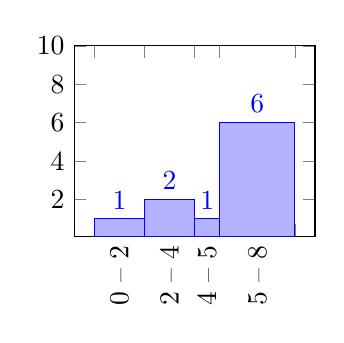
\begin{tikzpicture}
    \begin{axis}[
%        timeseriesrel,
        height=4cm,
        %width=10cm,scale only axis, height=5cm,
        ymax = 10,
        xtick = data,
        xticklabel interval boundaries,
        x tick label style= {rotate=90,anchor=east},
        x label style ={ at={(1,0)},left,yshift=0pt},
        ]
    \addplot[ybar interval,blue,fill=blue!30!white] coordinates{
        (0,1)
        (2,2)
        (4,1)
        (5,6)
        (8,6)
    }; 
    % \addlegendentry{Increments}

    \node[color=blue,above] at (axis cs:1,1) {1};
    \node[color=blue,above] at (axis cs:3,2) {2};
    \node[color=blue,above] at (axis cs:4.5,1) {1};
    \node[color=blue,above] at (axis cs:6.5,6) {6};
    \end{axis}
  \end{tikzpicture}
  \caption{Gràfic de barres}
    \label{fig:model:comptador-formes:barres}
  \end{subfigure}

  \begin{subfigure}{0.3\textwidth}
  \centering
  \begin{tikzpicture}
    \begin{axis}[
        timeseriesrel,
        title=$S_\Delta$
        ]
    \addplot[blue] coordinates {
        (0,0)
        (2,1)
        (2,0)
        (4,2)
        (4,0)
        (5,1)
        (5,0)
        (8,6)
        (8,0)
    };
    %\addlegendentry{Valor relatiu}
    \addplot[only marks,mark=*,red] coordinates {
        (0,0)
        (2,1)
        (4,2)
        (5,1)
        (8,6)
    };
    %\addlegendentry{Punts de mesura}
    \end{axis}
  \end{tikzpicture}
  \caption{Valor relatiu}
    \label{fig:model:comptador-formes:relatiu}
  \end{subfigure}
  \begin{subfigure}{0.3\textwidth}
  \centering
  \begin{tikzpicture}
    \begin{axis}[
        timeseriesrel,
        title=$S_v$,
        ymax=2.3,
        ]
    \addplot[const plot mark right,blue] coordinates {
        (0,0)
        (2,0.5)
        (4,1)
        (5,1)
        (8,2)
    };
    %\addlegendentry{Velocitat mitjana}

   \addplot[only marks,mark=*,red] coordinates {
        (0,0)
        (2,0.5)
        (4,1)
        (5,1)
        (8,2)
    };
    %\addlegendentry{Punts de mesura}

    \end{axis}
  \end{tikzpicture}
  \caption{Velocitat}
    \label{fig:model:comptador-formes:velocitat}
   \end{subfigure}
  \begin{subfigure}{0.3\textwidth}
  \centering
  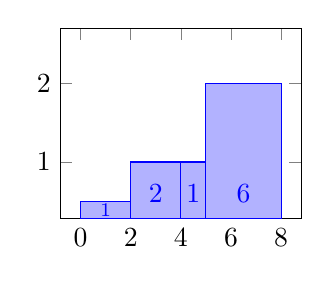
\begin{tikzpicture}
    \begin{axis}[
        height=4cm,
        ymax=2.7,
        ]
    \addplot[ybar interval,blue,fill=blue!30!white,mark=none] coordinates {
        (0,0.5)
        (2,1)
        (4,1)
        (5,2)
        (8,2)
    };
    %\addlegendentry{distribució d'increments}

    \node[color=blue] at (axis cs:1,0.39) {\scriptsize 1};
    \node[color=blue] at (axis cs:3,0.6) {2};
    \node[color=blue] at (axis cs:4.5,0.6) {1};
    \node[color=blue] at (axis cs:6.5,0.6) {6};
     \end{axis}
  \end{tikzpicture}
  \caption{Histograma}
  \label{fig:model:comptador-formes:histograma}
  \end{subfigure}

  \caption{Formes d'un comptador monòton}
  \label{fig:model:comptador-formes}
\end{figure}



Les magnituds ofereixen la informació d'una forma: l'estat de la
variable. A la \autoref{fig:model:magnitud} es mostra aquesta forma
amb una sèrie temporal d'exemple: $S_a = \{(0,0),(2,1),(3,
1{,}5),(4,0),(5,2),(8,2)\}$. De manera general, el valor d’una
magnitud física és defineix com el producte d’un valor numèric per una
unitat.


Els comptadors poden oferir la informació de diverses formes : en
valor absolut, en valor relatiu i en velocitat. A la
\autoref{fig:model:comptador-formes} es mostren aquestes formes amb
tres sèries temporals d'exemple: $S_a =
\{(0,0),(2,1),(4,3),(5,4),(8,10)\}$ són els valors absoluts del
comptador, $S_\Delta = \{(0,0)\} \cup
\glssymbol{not:sgst:gradient}(S_a) =
\{(0,0),(2,1),(4,2),(5,1),(8,6)\}$ són els valors relatius del
comptador i $S_v = S_\Delta /
\glssymbol{not:sgst:gradient}(\glssymbol{not:sgst:duplica-t}(S_\Delta))
= \{(0,0),(2,0{,}5),(4,1),(5,1),(8,2)\}$ són els valors de velocitat
del comptador, les unitats dels quals són de \emph{unitat$/$unitat de
  temps}.


El gràfic de valor absolut, en aquest cas es tracta d'un comptador
monòton creixent, mostra la interpolació lineal del valor acumulat que
va prenent la variable mesurada. A partir del valor absolut es poden
calcular els increments del comptador, és a dir la quantitat relativa
de cada període. En el gràfic d'increments es mostra en línia
discontínua la tendència dels increments, és a dir la interpolació
lineal del comptatge absolut com si el comptador fos una
magnitud, que cal no confondre amb el gràfic de valor relatiu que
mostra la interpolació lineal que va prenent la variable mesurada
relativament, és a dir amb el pas per zero com si a cada lectura
s'inicialitza de nou el valor acumulat del comptador. El gràfic de
velocitat mostra els pendents lineals del gràfic de valor relatiu, és
a dir la velocitat mitjana de comptatge a cada període.

El significat del gràfic de valor absolut i el d'increments es
visualitza bé en un gràfic de barres en el que l'eix vertical mostra
freqüència i en el que l'alçària de les barres mostra la quantitat que
ha augmentat el comptador a cada interval. En canvi el gràfic de valor
relatiu i el de velocitat es visualitzen més bé en un gràfic
d'histograma en el que l'eix vertical mostra densitat de freqüència i en el
que l'àrea de les barres equival a la quantitat comptada i l'alçària
de cada una mostra la velocitat del comptatge.


En conclusió, un comptador pot oferir les dades en qualsevol de les
tres formes i a partir d'una d'aquestes es poden calcular les
altres. També es possible d'aplicar les mateixes operacions a les
magnituds, és a dir calcular-ne els increments o la velocitat mitjana
de cada període, tenint en compte que aleshores es perd la referència
absoluta llevat que es conservi a part. La diferència principal
d'ambdós rau en el fet que l'objectiu de les magnituds és observar el
valor instantani d'una variable i per tant se sol obtenir en aquesta
forma mentre que l'objectiu dels comptadors és precisament el de
mesurar els comptatges totals de les variables en els períodes
seleccionats, i això es pot mostrar en les tres formes descrites. És a
dir, el tret semàntic de mètode d'adquisició està lligat al tipus
d'aparell de mesura: una magnitud ben mostrejada té informació
suficient per a calcular-ne els comptatges mentre que un comptador
inherentment mesura els totals però perd la noció del valor
instantani.

Altrament, tot i que els comptadors solen presentar un comportament
monòton, creixent o decreixent, també poden ser dobles i tenir
increments tant positius com negatius. Un efecte que també cal tenir
en compte dels comptadors, sobretot dels monòtons, és el fons
d'escala, que quan s'assoleix es torna a comptar des de l'inici i per
tant tenen un comportament semblant al de valor relatiu.

% * comptadors -> conservar totals (comptador: monòton, doble, relatiu)
% usualment són digitals en naturalesa (compten amb naturals) però també poden ser analògics (comptar amb reals, per exemple comptar el cabal d'aigua, l'energia consumida, etc.).

\begin{example}
  Un exemple de sèrie temporal amb tret de magnitud és la potència
  instantània elèctrica i un exemple de comptador és la quantitat
  d'energia elèctrica. Així doncs mesurant electricitat poden
  aparèixer sèries temporals amb els trets següents:

  \begin{itemize}
  \item Magnitud: potència instantània elèctrica.  Per exemple la
    sèrie $S_m$ amb unitats als valors de watts.
  \item Comptador de valor absolut: energia elèctrica. Per exemple la
    sèrie $S_a$ amb unitats als valors de watts$\times$hora o bé de
    joules.
  \item Comptador de valor relatiu: energia elèctrica amb posada a
    zero a cada lectura. Per exemple la sèrie $S_\Delta$ amb unitats
    als valors de watts$\times$hora o bé de joules.
  \item Comptador de velocitat: potència mitjana elèctrica. Per
    exemple la sèrie $S_v$ amb unitats als valors de watts o bé de
    watts$\times$hora$/$hora.
  \end{itemize}

  Si la potència instantània és periòdica es pot mostrejar
  correctament per a saber el total d'energia elèctrica, si no és
  periòdica difícilment es pot determinar la quantitat amb exactitud.
  En canvi, mentre que un aparell de comptatge mesura exactament la
  quantitat d'energia, no es pot recuperar la potència instantània si
  no es coneix quina forma té. 
\end{example}



\subsubsection{Temps}

Un segon tret semàntic de les sèries temporals també es deu al mètode
d'adquisició però en aquest cas segons la continuïtat del temps.

\textcite{furia10:modeling_time} distingeix entre temps dens
(\emph{dense time}) i temps discret (\emph{discrete time}) segons si
entre dos instants de temps n'hi pot haver un de tercer o si els
instants de temps son punts aïllats. Un exemple de domini del temps
com a conjunt dens són els reals $T\in \glssymbol{not:Rb}$ i com a
conjunt discret són els naturals $T\in \N$.
\textcite[cap.~3]{kopetz11:realtime} descriu conceptes similars tot i que els
anomena \emph{dense time} i \emph{sparse time} i ho fa des del punt de
vista d'esdeveniments de temps real. Així fa notar que els
esdeveniments es produeixen amb \emph{sparse time} quan hi ha un
sistema que controla el rellotge però que els esdeveniments que són
externs a aquest control sempre es produeixen amb \emph{dense time}.
% també parla dels processos amb representació cíclica del temps

Així, segons la perspectiva de sistema de coordenades temps continu,
el temps dens infereix als instants de temps un significat de punt
(\emph{timestamp}) mentre que el temps discret infereix un significat
de lapse de temps (\emph{time span}).  
Un cas particular de sèries temporals amb trets de temps
discret són les que tenen trets de seqüència. Les sèries temporals com
a seqüències són habituals en l'anàlisi de sèries temporals ja que són
una manera simple d'observar un conjunt de dades ordenades en el temps
sense determinar-ne exactament la distància temporal entre elles.


Un cas que observem amb tret de seqüència són les sèries temporals que
recullen agregacions d'intervals de temps. Per exemple una sèrie
temporal que recull les temperatures mitjanes de cada mes
$S=\{(\text{gen},10),(\text{feb},11),(\text{març},15),\dotsc\}$. En
aquest cas el temps és discret i té el domini
$T\in\{\text{gen},\text{feb},\text{març},\dotsc\}$ i cada instant de
temps es pot observar com un lapse que dura tot el mes. Això no
obstant, aquestes sèries temporals s'expressen amb més exactitud amb
temps dens, per exemple en el cas de les mitjanes s'hauran adquirit a
final de mes i per tant els instants de temps poden ser més precisos
$S=\{(\text{31-gen 23.59},10),(\text{28-feb 23.59},11),(\text{31-març
  23.59},15),\dotsc\}$.
% aquestes no són comptadors, no tenen forma de valor relatiu ni
% encara que tenen representació zoh/zohc/zohe no són velocitat perquè
% no tenen unitats de unitats/u.t.

Un cas que observem amb tret de seqüència són les sèries temporals que
recullen agregacions d'intervals de temps no continus.  Per exemple
una sèrie temporal que recull les temperatures mitjanes dels mesos
d'octubre
$S=\{(\text{oct98},15),(\text{oct99},10),(\text{oct00},13),\dotsc\}$.
En aquest cas el temps és discret i té el domini
$T\in\{\text{oct98},\text{oct99},\text{oct00},\dotsc\}$ i cada instant
de temps es pot observar com un lapse que dura tot un mes d'octubre
però no hi ha continuïtat del temps entre els mesos. Així doncs,
aquestes sèries temporals presenten més dificultats a l'hora
d'expressar-se amb temps dens, per exemple com en el cas anterior es
pot precisar amb els instants de temps
$S=\{(\text{31-oct-98},15),(\text{31-oct-99,10}),(\text{31-oct-00,13}),\dotsc\}$
o bé refermar-ho amb valors indefinits
$S=\{(\text{30-set-98},\infty),(\text{31-oct-98},15),(\text{30-set-99},\infty),(\text{31-oct-99,10}),\dotsc\}$,
però cal anar en compte amb les operacions que s'hi apliquin ja que
poden no adequar-se a la semàntica si no tenen en compte aquesta
discontinuïtat del temps. 
% De la mateixa manera, les operacions d'anàlisi de seqüències
% temporals poden no ser totalment certes si no han tingut en compte
% que el temps és continu, o discret però sense salts.



\subsubsection{Intervals de temps}

Finalment, hi ha dades que s'anoten en intervals de temps en comptes
d'instants de temps. Aquests casos pertanyen al model d'intervals de
temps, el qual és diferent del de sèries temporals. Algunes dades en
intervals de temps es poden expressar perfectament en sèries temporals
però altres no resulta tan còmode. Vegem-ne alguns exemples.

%El temps pot ser tant dens, $T\in\R$, com discret

Un primer exemple és el tipus d'interès que fixa el Banc Central
Europeu. En aquest cas es fixen valors cadascun dels quals és vàlid
durant un determinat interval de temps. Una expressió d'exemple
possible, sense detallar el model d'intervals temporals, és
$I=\{([1,2),0.25),([2,4),0.50),([5,7),0.75)\}$ amb els valors en
unitats de tant per cent. Es pot expressar fàcilment en sèrie temporal
$S=\{(1,0.25),(2,0.50),(4,0.75),(7,\infty)\}$, i acompanyar-ho amb una
representació adequada com la ZOH (v.~\autoref{def:sgst:zoh}).


Un segon exemple és una agenda, la qual fixa tasques en intervals de
temps futurs. Per exemple expressat en intervals temporals
$I=\{([7,8),\text{transport}),([8,15),\text{feina}),([17,18),
\text{dentista})\}$. També com en el cas anterior es pot expressar en
sèrie temporal $S=\{(7,\text{transport}),(8,\text{feina}), (15,\infty)
,(17,\text{dentista}), (18,\infty)\}$. Tot i així, per a aquest
exemple la sèrie temporal no és còmode i és millor el model
d'intervals temporals, el qual està més orientat a expressar
el temps de validesa de cada tasca.



%- Per exemple un control de versions 

%- altre ex. cas d'una partitura musical  $S=\{(1,do),(2,re),(4,silenci),(5,fa),(7,silenci)\}$  es pot descriure com una sèrie temporal conjuntament amb la respresentació ZOH però seria millor fer servir el model d'intervals temporals... $I=\{([1,2),do),([2,4),re),([5,7),fa)\}$







\subsection{Graf i funció temporal de representació}
\label{sec:model:repr}

Una sèrie temporal és la representació discreta d'una funció contínua;
la qual és una funció temporal atès que depèn del temps. El model de
SGST definit formalitza la sèrie temporal com aquesta
representació discreta. Però a partir d'una sèrie temporal es pot
voler interpretar quina era la funció contínua original; és a dir
obtenir nous valors segons una funció a la que s'anomena graf d'una
funció (\emph{graph of a function}), en el sentit de gràfic
(\emph{plot}) que cal no confondre amb els grafs d'arestes i vèrtexs
(\emph{vertex-edge graph}).

\begin{definition}[Graf d'una sèrie temporal]%an. graph
  Sigui $S=\{m_0,\ldots,m_k\}$ una sèrie temporal i $T$ un domini del
  temps, es defineix el graf de la sèrie temporal
  $\glssymboldef{not:sgst:graf} S(t)$ com un conjunt de parells
  ordenats $(t,S(t))$ : $\glssymboldef{not:sgst:graf} S(t) = \{ (t,S(t)) |
  t\in T \}$ a on $S(t)$ és una funció de representació de la sèrie
  temporal.
\end{definition}

Per a calcular el graf d'una sèrie temporal es necessita una funció de
representació. Mentre que la funció que permet canviar d'una funció
contínua a una sèrie temporal s'anomena procés d'adquisició o
mostreig, la funció que permet canviar d'una sèrie temporal a una
funció contínua l'anomenem funció de representació.  Així doncs,
donada una sèrie temporal es poden definir funcions amb el temps com a
variable que calculin nous valors a partir de les mesures
emmagatzemades.
\begin{definition}[Funció de representació]
  Sigui $S=\{m_0,\ldots,m_k\}$ una sèrie temporal, es defineix $S(t)$
  com la funció de representació de la sèrie temporal contínuament al
  llarg del temps $t$; és a dir que per cada instant de temps la
  funció pren un valor: $\forall t\in T: v(t) = S(t)$. 

  Atenent a les operacions de càlcul que es facin per a obtenir $S(t)$
  diem que hi ha diverses funcions de representació. Així per a cada
  funció de representació indicarem a quina ens referim amb un
  superíndex \glsdispdef{not:sgst:frepr}{$S^r(t)$} a on
  \glssymboldef{not:sgst:repr} és el nom d'una funció de representació
  de la sèrie temporal.
\end{definition}

La utilitat de les funcions de representació és diversa i per això les
operacions de càlcul poden ser qualssevol. Una funció de representació
es pot utilitzar per a interpolar valors d'una sèrie temporal però
també per a extrapolar-los i fer prediccions o per a canviar la
resolució de la sèrie temporal. També es pot utilitzar com a tècnica
d'aproximar la sèrie temporal a la funció original; és a dir trobar
una funció de representació que es correspongui amb la funció contínua
que més s'aproxima a la funció temporal original.


El lligam entre una sèrie temporal i la seva representació no és fix;
és a dir que donada una sèrie temporal es pot representar amb una
funció o amb una altra segons convingui.  Encara que en alguns àmbits,
per exemple a teoria del senyal o en algunes aplicacions de l'anàlisi
de sèries temporals, l'objectiu és cercar la parella de sèrie temporal
i representació que més s'aproxima a la funció contínua original; en
altres àmbits, com per exemple el del model multiresolució que definim
posteriorment, l'objectiu està més orientat a utilitzar
representacions de les sèries temporals segons els càlculs que es
volen fer o segons la naturalesa que s'assumeixi de la sèrie temporal.


No obstant, les funcions de representació s'han d'utilitzar amb
criteri. Per exemple la naturalesa de la sèrie temporal indueix a unes
possibles operacions de càlcul que es poden realitzar, per tant
l'aplicació de qualsevol funció de representació a la sèrie temporal
pot donar resultats incoherents. O bé un altre exemple és aplicar
càlculs successius a una sèrie temporal seguint diferents funcions de
representació.  

Així i tot, en la formalització del model de funcions de
representacions no hi definim cap criteri en concret per a, així,
donar llibertat en les possibilitats de càlcul amb les sèries
temporals. Al capítol \todo{ref} d'estat actual ja s'ha vist que en
l'anàlisi de sèries temporals hi ha diversitat en els algoritmes de
representació que s'utilitzen.
% entre els quals destaquen els que es basen en aproximació als valors
% de la sèrie temporal. Aquí ens centrem en els algoritmes
% d'interpolació exactes, els quals són més senzills de comprendre.

,
A continuació, definim diverses funcions de representació per a
exemplificar-ne l'ús. Les agrupem per algunes de les seves
característiques, a les qual podem veure com famílies de funcions de
representació, i de cada una en definim les més representatives. Per a
cada definició una oferim, quan es pugui, dues expressions
equivalents: una en matemàtica contínua, que ajuda a comprendre el
significat, i una en matemàtica discreta, que utilitza l'àlgebra del
model de SGST.



\subsubsection{Funcions parcials}
\todo{no sé si aporten res les parcials? cal acabar la secció d'agregadors dels SGSTM i repensar això}
\todo{Les funcions parcials tenen a veure amb representacions per als casos que tractem les sèries temporals amb operadors de conjunts o seqüències. En aquests casos no hi ha una interpretació clara del què hi ha entre les mesures. Si des de les representacions volem observar aquests casos hem de definir funcions parcials, les quals no són totalment contínues en el temps}


Primerament, definim una funció de representació anomenada discreta
pura que no és totalment contínua en el temps sinó que és una funció
parcial.
\begin{definition}[Funció de representació discreta pura]
  Sigui $S=\{m_0,\ldots,m_k\}$ una sèrie temporal, es defineix
  $S^d(t)$ com la funció de representació discreta pura de la sèrie
  temporal $\forall m \in S: S^d(t) =
  \begin{cases}
    V(m) & \text{si }  t=T(m) \\
    \text{no definit} & \text{altrament}
  \end{cases}$.
\end{definition}

Aquest és un cas especial de funció de representació perquè permet que
el graf de la sèrie temporal sigui equivalent a les mesures de la
sèrie temporal: $\glssymbol{not:sgst:graf} S^d(t) \equiv
\{m_0,\ldots,m_k\}$.

Es poden definir altres funcions de representació de la família
parcial, però presenten el problema que el domini queda restringit a
un subconjunt $T'$ del domini temps $T$; el domini queda restringit
als instants de temps elegits $T'$ ja que per qualsevol altre instant de
$T$ no hi ha imatge definida.

Així doncs, és millor definir funcions totals que sempre seran
funcions ben-definides per al domini temps.
\todo{sinó, es poden trobar equivalents en les contínues?}



\begin{example}[Sèrie temporal amb representació discreta pura]
  Sigui la sèrie temporal $S=\{ (3,1), (4,3), (6,2), (9,1) \}$, el
  graf de la representació discreta pura és $\glssymbol{not:sgst:graf}
  S^d(t)=\{ (3,1), (4,3), (6,2), (9,1) \}$, el qual es mostra a la
  \autoref{fig:model:repr:d}.


  \begin{figure}[tp]
  \centering
  \begin{tabular}[c]{|c|c|}
    \multicolumn{2}{c}{$S$} \\ \hline
    $t$  & $v$ \\ \hline
    3  & 1 \\
    4  & 3 \\
    6  & 2 \\
    9  & 1 \\ \hline
  \end{tabular} \qquad
  \begin{tikzpicture}[baseline=(current bounding box.center)]
    \begin{axis}[
        timeseriesrel,
        title=$S^d$,
        ]
    \addplot[mark=*,blue,only marks] coordinates { 
        (3,1) 
        (4,3)
        (6,2)
        (9,1)
    };




    \end{axis}
   \end{tikzpicture}
   \caption{Taula d'una sèrie temporal $S$ i
     $\glssymbol{not:sgst:graf} S^d(t)$}
  \label{fig:model:repr:d}
  \end{figure}
\end{example}




\subsubsection{A impulsos}

Una família de funcions contínues que recorda a la funció discreta són
les funcions d'impulsos (\emph{impulse train function}).  A
continuació ho exemplifiquem amb una representació que anomenem delta
($\delta$) perquè es basa en la funció delta de Dirac, la qual val
zero a tot arreu excepte en el punt zero.

\begin{definition}[Funció de representació delta]
  Sigui $S=\{m_0,\ldots,m_k\}$ una sèrie temporal i $T$ el domini del
  temps, es defineix $S^\delta(t)$ com la funció de representació
  delta al llarg del temps, $\forall m \in S:$
  \begin{align*}
    S^\delta(t) = &  \\
    = & \sum_{t\in T} V(m) \delta(t-T(m)): \delta(t)= 
      \begin{cases}
        1 & \text{si }  t=0 \\
        0 & \text{altrament}
      \end{cases} \\
    = & \begin{cases}
      V(m) & \text{si }  t=T(m) \\
      0 & \text{altrament}
    \end{cases}
         \end{align*}.
\end{definition}



\begin{example}[Sèrie temporal amb representació delta]
  Sigui la sèrie temporal $S=\{ (3,1), (4,3), (6,2), (9,1) \}$, la
  seva representació delta és $S^\delta(t) = 0 +1\delta(t-3)
  +3\delta(t-4) +2\delta(t-6) +1\delta(t-9)$. El graf d'aquesta
  representació, $\glssymbol{not:sgst:graf} S^\delta(t)$, es mostra a
  la \autoref{fig:model:repr:delta}.


  \begin{figure}[tp]
  \centering
  \begin{tabular}[c]{|c|c|}
    \multicolumn{2}{c}{$S$} \\ \hline
    $t$  & $v$ \\ \hline
    3  & 1 \\
    4  & 3 \\
    6  & 2 \\
    9  & 1 \\ \hline
  \end{tabular} \qquad
  \begin{tikzpicture}[baseline=(current bounding box.center)]
    \begin{axis}[
        timeseriesrel,
        title=$S^\delta$,
        xmin=0,
        xmax=11,
        xtickmin=0,
        xtickmax=10,
        try min ticks=6,
        ]
    \addplot[mark=*,blue,ycomb] coordinates { 
        (3,1) 
        (4,3)
        (6,2)
        (9,1)
    };

    \addplot[mark=o,blue,only marks] coordinates { 
        (3,0)
        (4,0)
        (6,0)
        (9,0)
    };


    \pgfplotsextra{%
      \pgfpathmoveto{\pgfplotspointaxisxy{0.5}{0}}%
      \pgfpathlineto{\pgfplotspointaxisxy{12}{0}}%
      \pgfsetarrowsstart{latex}
      \pgfsetarrowsend{latex}
      \pgfsetcolor{blue}
      \pgfusepath{stroke}%
    }


    \end{axis}
   \end{tikzpicture}
   \caption{Taula d'una sèrie temporal $S$ i
     $\glssymbol{not:sgst:graf} S^\delta(t)$}
  \label{fig:model:repr:delta}
  \end{figure}
\end{example}


\subsubsection{A trossos constants}

Una altra família de funcions són les que es basen en funcions
definides a trossos constants (\emph{piecewise constant functions}).
A continuació ho exemplifiquem amb quatre representacions basades en la
funció graó (\emph{step function} o \emph{staircase function}) atenent
a quatre de les possibles continuïtats en els intervals de temps. 


A les definicions següents s'utilitza la notació de funció
característica $\glssymbol{not:Ia}_A(t)$ per a indicar quan un instant
de temps pertany a un determinat interval de temps:
\[
\glssymbol{not:Ia}_A(t) = 
   \begin{cases}
      1 & \text{si } t\in A \\
      0 & \text{altrament}
    \end{cases}
\]



%(\emph{right-continuous})
En primer lloc, definim una representació en base a funcions graó
contínues per la dreta. L'anomenem representació \emph{zero-order
  hold} (ZOH) a causa de la semblança que té amb el model utilitzat en
electrònica per a reconstruir senyals, el qual consisteix en mantenir
constant cada valor fins al proper.
\begin{definition}[Funció de representació \emph{zero-order hold}]
  \label{def:sgst:zoh}
  Sigui $S=\{m_0,\ldots,m_k\}$ una sèrie temporal i $T$ el domini del
  temps, es defineix $S^\text{ZOH}(t)$ com la funció de representació
  \emph{zero-order hold} al llarg del temps, $\forall m \in S:$
  \begin{align*}
    S^\text{ZOH}(t) = &  \\
    = & \sum_{t\in T} V(m) \glssymbol{not:Ia}_{\big[T(m), T(\glssymbol{not:sgst:next}(m)) \big)}(t)\\
    = & \begin{cases}
      0 & \text{si }  t<T(\min(S)) \\
      V(m) & \text{si } t\in
      \big[T(m),T(\glssymbol{not:sgst:next}(m))\big)
    \end{cases}
         \end{align*}.
\end{definition}



En segon lloc, definim una representació en base a funcions graó
contínues per l'esquerra. L'anomenem representació \emph{zero-order
  hold} cap enrere (ZOHE) perquè consisteix en mantenir constant cada
valor fins al predecessor. Una representació similar s'utilitza a
\gls{RRDtool} \parencite{lisa98:oetiker}.
\begin{definition}[Funció de representació \emph{zero-order hold} cap
  enrere]%\emph{zero-order hold backwards}(zohe%from \emph{zero-order
         %hold everted}
  \label{def:model:zohe}
  Sigui $S=\{m_0,\ldots,m_k\}$ una sèrie temporal i $T$ el domini del
  temps, es defineix $S^\text{ZOHE}(t)$ com la funció de representació
  \emph{zero-order hold} cap enrere al llarg del temps, $\forall m \in S:$
  \begin{align*}
    S^\text{ZOHE}(t) = &  \\
    = & \sum_{t\in T} V(m) \glssymbol{not:Ia}_{\big(T(\glssymbol{not:sgst:prev}(m)),T(m)\big]}(t) \\
    = & \begin{cases}
      0 & \text{si }  t > T(\max(S)) \\
      V(m) & \text{si } t\in \big(T(\glssymbol{not:sgst:prev}(m)),T(m)\big]
    \end{cases}
         \end{align*}.
\end{definition}



En tercer lloc, definim una representació en base a funcions graó
contínues per la dreta centrades en l'interval. L'anomenem
representació \emph{zero-order hold} centrada en l'interval (ZOHC).
\begin{definition}[Funció de representació \emph{zero-order hold}
  centrada en l'interval]
  Sigui $S=\{m_0,\ldots,m_k\}$ una sèrie temporal i $T$ el domini del
  temps, es defineix $S^\text{ZOHC}(t)$ com la funció de representació
  \emph{zero-order hold} centrada en l'interval al llarg del temps,
  $\forall m \in S:$
  \begin{align*}
    S^\text{ZOHC}(t) = &  \\
   = & \sum_{t\in T} V(m) \glssymbol{not:Ia}_{\left[
        \frac{T(\glssymbol{not:sgst:prev}(m))+T(m)}{2},
        \frac{T(m)+T(\glssymbol{not:sgst:next}(m))}{2}
      \right)}(t) \\
    = & V(m): t\in \left[
        \frac{T(\glssymbol{not:sgst:prev}(m))+T(m)}{2},
        \frac{T(m)+T(\glssymbol{not:sgst:next}(m))}{2} \right)
         \end{align*}.
\end{definition}




En quart lloc, representem la sèrie temporal en base a la funció
rectangular. La funció rectangular és un cas especial de les funcions
graó a on s'especifiquen valors simètrics per als punts de
discontinuïtat. Definim el rectangle amb manteniment del valor cap a
la dreta, de manera similar al ZOH, tot i que també es possible
definir altres translacions del rectangle com s'ha fet per la funció
graó en el cas del ZOHE i el ZOHC.
\begin{definition}[Funció de representació rectangular]
  Sigui $S=\{m_0,\ldots,m_k\}$ una sèrie temporal i $T$ el domini del
  temps, es defineix $S^\text{rect}(t)$ com la funció de representació
  rectangular al llarg del temps, $\forall m \in S:$
  \begin{align*}
    S^\text{rect}(t) = &  \\
    = & \sum_{t\in T} V(m) \operatorname{rect}(t):  \operatorname{rect}(t) = 
    \begin{cases}
      1 & \text{si } t\in \big(T(m),T(\glssymbol{not:sgst:next}(m))\big) \\
      \frac{1}{2}& \text{si } t = T(m) \vee t=T(\glssymbol{not:sgst:next}(m)) \\
      0 & \text{altrament}
    \end{cases} \\
    = & \begin{cases}
      0 & \text{si }  t<T(\min(S)) \\
      V(m) & \text{si } t\in \big(T(m),T(\glssymbol{not:sgst:next}(m))\big) \\
      \frac{V(m)+V(\ant(m))}{2} & \text{si } t = T(m) \wedge t > T(\min(S)) \\
      \frac{V(m)}{2} & \text{si } t = T(\min(S)) \\
    \end{cases}
         \end{align*}.
\end{definition}


% En la representació rectangular només hem definit un cas semblant al
% del la representació ZOH. També podríem definir variacions de la
% rectangular com s'ha fet per la ZOH: la ZOHE i la ZOHC. 
% La variació entre la ZOH i la ZOHC o la ZOHE no és només una translació. 



\begin{example}[Sèrie temporal amb representació ZOHE]
  Sigui la sèrie temporal $S=\{ (3,1), (4,3), (6,2), (9,1) \}$, la
  seva representació ZOHE és $S^\text{ZOHE}(t) =
  1\glssymbol{not:Ia}_{(-\infty,3]} +3\glssymbol{not:Ia}_{(3,4]}
  +2\glssymbol{not:Ia}_{(4,6]} +1\glssymbol{not:Ia}_{(6,9]}
  +0\glssymbol{not:Ia}_{(9,+\infty)}$. El graf d'aquesta
  representació, $\glssymbol{not:sgst:graf} S^\text{ZOHE}(t)$, es
  mostra a la \autoref{fig:model:repr:zohe}.


  \begin{figure}[tp]
  \centering
  \begin{tabular}[c]{|c|c|}
    \multicolumn{2}{c}{$S$} \\ \hline
    $t$  & $v$ \\ \hline
    3  & 1 \\
    4  & 3 \\
    6  & 2 \\
    9  & 1 \\ \hline
  \end{tabular} \qquad
  \begin{tikzpicture}[baseline=(current bounding box.center)]
    \begin{axis}[
        timeseriesrel,
        title=$S^\text{ZOHE}$,
        xmin=0,
        xmax=11,
        xtickmin=0,
        xtickmax=10,
        try min ticks=6,
        ]
    \addplot[mark=*,blue,const plot mark right] coordinates { 
        (3,1) 
        (4,3)
        (6,2)
        (9,1)
    };

    \addplot[mark=o,blue,only marks] coordinates { 
        (3,3)
        (4,2)
        (6,1)
        (9,0)
    };

    \pgfplotsextra{%
      \pgfpathmoveto{\pgfplotspointaxisxy{9}{1}}%
      \pgfpathlineto{\pgfplotspointaxisxy{9}{0}}%
      \pgfsetcolor{blue}
      \pgfusepath{stroke}%
    }

    \pgfplotsextra{%
      \pgfpathmoveto{\pgfplotspointaxisxy{9}{0}}%
      \pgfpathlineto{\pgfplotspointaxisxy{12}{0}}%
      \pgfsetarrowsend{latex}
      \pgfsetcolor{blue}
      \pgfusepath{stroke}%
    }

    \pgfplotsextra{%
      \pgfpathmoveto{\pgfplotspointaxisxy{3}{1}}%
      \pgfpathlineto{\pgfplotspointaxisxy{0.5}{1}}%
      \pgfsetarrowsend{latex}
      \pgfsetcolor{blue}
      \pgfusepath{stroke}%
    }

    \end{axis}
   \end{tikzpicture}
   \caption{Taula d'una sèrie temporal $S$ i
     $\glssymbol{not:sgst:graf} S^\text{ZOHE}(t)$}
  \label{fig:model:repr:zohe}
  \end{figure}
\end{example}



\begin{example}[Sèrie temporal amb representació rectangular]
  Sigui la sèrie temporal $S=\{ (3,1), (4,3), (6,2), (9,1) \}$, la
  seva representació rectangular és $S^\text{rect}(t) =
  0\glssymbol{not:Ia}_{(-\infty,3)} +0{,}5\glssymbol{not:Ia}_{[3,3]}
  +1\glssymbol{not:Ia}_{(3,4)} +2\glssymbol{not:Ia}_{[4,4]}
  +3\glssymbol{not:Ia}_{(4,6)} +2{,}5\glssymbol{not:Ia}_{[6,6]}
  +2\glssymbol{not:Ia}_{(6,9)} +1{,}5\glssymbol{not:Ia}_{[9,9]}
  +1\glssymbol{not:Ia}_{(9,+\infty)}$. El graf d'aquesta
  representació, $\glssymbol{not:sgst:graf} S^\text{rect}(t)$, es
  mostra a la \autoref{fig:model:repr:rect}.


  \begin{figure}[tp]
  \centering
  \begin{tabular}[c]{|c|c|}
    \multicolumn{2}{c}{$S$} \\ \hline
    $t$  & $v$ \\ \hline
    3  & 1 \\
    4  & 3 \\
    6  & 2 \\
    9  & 1 \\ \hline
  \end{tabular} \qquad
  \begin{tikzpicture}[baseline=(current bounding box.center)]
    \begin{axis}[
        timeseriesrel,
        title=$S^\text{rect}$,
        xmin=0,
        xmax=11,
        xtickmin=0,
        xtickmax=10,
        try min ticks=6,
        ]
    \addplot[mark=o,blue,const plot mark left] coordinates { 
        (3,1) 
        (4,3)
        (6,2)
        (9,1)
    };

    \addplot[mark=o,blue,only marks] coordinates { 
        (3,0)
        (4,1)
        (6,3)
        (9,2)
    };

    \addplot[mark=*,blue,only marks] coordinates { 
        (3,0.5)
        (4,2)
        (6,2.5)
        (9,1.5)
    };

    \pgfplotsextra{%
      \pgfpathmoveto{\pgfplotspointaxisxy{3}{1}}%
      \pgfpathlineto{\pgfplotspointaxisxy{3}{0}}%
      \pgfsetcolor{blue}
      \pgfusepath{stroke}%
    }

    \pgfplotsextra{%
      \pgfpathmoveto{\pgfplotspointaxisxy{9}{1}}%
      \pgfpathlineto{\pgfplotspointaxisxy{12}{1}}%
      \pgfsetarrowsend{latex}
      \pgfsetcolor{blue}
      \pgfusepath{stroke}%
    }

    \pgfplotsextra{%
      \pgfpathmoveto{\pgfplotspointaxisxy{3}{0}}%
      \pgfpathlineto{\pgfplotspointaxisxy{0.5}{0}}%
      \pgfsetarrowsend{latex}
      \pgfsetcolor{blue}
      \pgfusepath{stroke}%
    }

    \end{axis}
   \end{tikzpicture}
   \caption{Taula d'una sèrie temporal $S$ i
     $\glssymbol{not:sgst:graf} S^\text{rect}(t)$}
  \label{fig:model:repr:rect}
  \end{figure}

\end{example}






\subsubsection{A trossos lineals}

Una família de funcions d'un ordre superior a les de trossos constants
són les que es basen en funcions definides a trossos lineals
(\emph{piecewise linear functions}).  A continuació ho exemplifiquem
amb una representació basada en la funció triangular (\emph{triangular
  function}). Seguint amb l'analogia electrònica l'anomenem
representació \emph{first-order hold}(FOH), el qual consisteix en
interpolar linealment cada valor fins al proper.


La definició del FOH amb funcions matemàtiques contínues es construeix
a partir de la funció triangular $\operatorname{tri}(t)$
\[
\operatorname{tri}(t) = 
\begin{cases}
  1-|t| & \text{si } |t| < 1\\
  0 & \text{altrament}
\end{cases}
\]

Per al cas particular de sèries temporals regulars
(v.~\autoref{def:st:regular}), es pot utilitzar directament la funció
triangular general.  Sigui $S_R=\{m_0,\ldots,m_k\}$ una sèrie temporal
regular amb període $P$ i sigui $T$ el domini del temps, es defineix
$S^\text{FOH}_ R(t)$ com la funció de representació \emph{first-order
  hold} al llarg del temps, $\forall m \in S:$
\[
S_ R^\text{FOH}(t) = \sum_{t\in T} V(m)
\operatorname{tri}\left(\frac{t-T(m)}{P}\right)
\]



Per al cas general, tant per a sèries temporals regulars com per a no
regulars, s'ha de construir a partir de funcions triangulars no
simètriques:
\[
\operatorname{tri}^{-1}(t) = 
\begin{cases}
  1-|t| & \text{si } -1 < t < 0\\
  0 & \text{altrament}
\end{cases}
\quad
\operatorname{tri}^1(t) = 
\begin{cases}
  1-|t| & \text{si } 0 \leq t < 1\\
  0 & \text{altrament}
\end{cases}
\]


\begin{definition}[Funció de representació \emph{first-order hold}]
  Sigui $S=\{m_0,\ldots,m_k\}$ una sèrie temporal i $T$ el domini del
  temps, es defineix $S^\text{FOH}(t)$ com la funció de representació
  \emph{first-order hold} al llarg del temps, $\forall m \in S:$
  \begin{align*}
    :\; & x_1=T(m), y_1=V(m), \\
    & m_2=\glssymbol{not:sgst:next}(m), x_2=T(m_s), y_2=V(m_s),\\
    & m_0=\glssymbol{not:sgst:prev}(m), x_0=T(m_a), y_0=V(m_a) :\\
    S^\text{FOH}(t) = & \\
    = & \sum_{t\in T} y_1
    \left(
      \operatorname{tri}^{-1}\left(\frac{t-x_1}{x_1-x_0}\right)
      +\operatorname{tri}^1\left(\frac{t-x_1}{x_2-x_1}\right)
    \right)  \\
    = & \begin{cases}
      V(\min(S)) & \text{si } t<T(\min(S) )\\
      V(\max(S)) & \text{si } t> T(\max(S))  \\
      \frac{y_2-y_1}{x_2-x_1}(t-x_1)+y_1 & \text{si } t\in
      \big[x_1,x_2\big) \wedge t \leq T(\max(S))
    \end{cases}
  \end{align*}.
\end{definition}




\begin{example}[Sèrie temporal amb representació FOH]
  Sigui la sèrie temporal $S=\{ (3,1), (4,3), (6,2), (9,1) \}$, la
  seva representació amb FOH és $S^\text{FOH}(t) =
  1\operatorname{tri}^{-1}\left(\frac{t-3}{3-(-\infty)}\right) +
  1\operatorname{tri}^1\left(\frac{t-3}{4-3}\right)
  +3\operatorname{tri}^{-1}\left(\frac{t-4}{4-3}\right) +
  3\operatorname{tri}^1\left(\frac{t-4}{6-4}\right)
  +2\operatorname{tri}^{-1}\left(\frac{t-6}{6-4}\right) +
  2\operatorname{tri}^1\left(\frac{t-6}{9-6}\right)
  +1\operatorname{tri}^{-1}\left(\frac{t-9}{9-6}\right) +
  1\operatorname{tri}^1\left(\frac{t-9}{+\infty-9}\right)$. El graf
  d'aquesta representació, $\glssymbol{not:sgst:graf}
  S^\text{FOH}(t)$, es mostra a la
  \autoref{fig:model:repr:foh}.


  \begin{figure}[tp]
  \centering
  \begin{tabular}[c]{|c|c|}
    \multicolumn{2}{c}{$S$} \\ \hline
    $t$  & $v$ \\ \hline
    3  & 1 \\
    4  & 3 \\
    6  & 2 \\
    9  & 1 \\ \hline
  \end{tabular} \qquad
  \begin{tikzpicture}[baseline=(current bounding box.center)]
    \begin{axis}[
        timeseriesrel,
        title=$S^\text{FOH}$,
        xmin=0,
        xmax=11,
        ymin=0,
        xtickmin=0,
        xtickmax=10,
        try min ticks=6,
        ]
    \addplot[mark=*,blue] coordinates { 
        (3,1) 
        (4,3)
        (6,2)
        (9,1)
    };

    \addplot[lightgray] coordinates { 
        (3,1) 
        (4,0)
    };
     \addplot[lightgray] coordinates { 
        (3,0)
        (4,3)
        (6,0)
    };
    \addplot[lightgray] coordinates { 
        (4,0)
        (6,2)
        (9,0)
    };
    \addplot[lightgray] coordinates { 
        (6,0)
        (9,1)
    };



    \pgfplotsextra{%
      \pgfpathmoveto{\pgfplotspointaxisxy{9}{1}}%
      \pgfpathlineto{\pgfplotspointaxisxy{12}{1}}%
      \pgfsetarrowsend{latex}
      \pgfsetcolor{blue}
      \pgfusepath{stroke}%
    }

    \pgfplotsextra{%
      \pgfpathmoveto{\pgfplotspointaxisxy{3}{1}}%
      \pgfpathlineto{\pgfplotspointaxisxy{0.5}{1}}%
      \pgfsetarrowsend{latex}
      \pgfsetcolor{blue}
      \pgfusepath{stroke}%
    }

    \end{axis}
   \end{tikzpicture}
   \caption{Taula d'una sèrie temporal $S$ i
     $\glssymbol{not:sgst:graf} S^\text{FOH}(t)$}
  \label{fig:model:repr:foh}
  \end{figure}

\end{example}





\subsubsection{D'ajustament lineal de corbes}

Una família de funcions diferents als casos anteriors són les funcions
d'ajustament lineal de corbes amb polinomis.  L'ajustament de corbes
(\emph{curve fitting}) és una tècnica que es basa en l'aproximació als
punts donats, a diferència de les funcions definides a trossos que es
basen en interpolacions que passin exactament pels punts donats.  A
continuació ho exemplifiquem amb una representació basada en
l'aproximació lineal per mínims quadrats; és a dir la regressió lineal
(\emph{linear regression}).


Definim una representació que consisteix en trobar la recta d'ajust
mínima quadràtica a les mesures de la sèrie temporal. L'anomenem
representació \emph{lineal} de la sèrie temporal.
\begin{definition}[Funció de representació lineal]
  Sigui $S=\{m_0,\ldots,m_k\}$ una sèrie temporal i $T$ el domini del
  temps, es defineix $S^\text{lineal}(t)$ com la funció de
  representació de regressió lineal al llarg del temps, $\forall m \in
  S:$
  \begin{align*}
    S^\text{lineal}(t) = & \alpha + \beta t \\
    :\; & 
    \left[\begin{array}{c}
        \alpha \\
        \beta
      \end{array}\right] 
    = (A^TA)^{-1}A^TB, \\
    & A=\left[\begin{array}{cc}
        1 & T(m_0) \\
        \vdots & \vdots \\
        1 & T(m_k)
      \end{array}\right],
    B=\left[\begin{array}{c}
        V(m_0) \\
        \vdots \\
        V(m_k)
      \end{array}\right]       
   \end{align*}.
\end{definition}



\begin{example}[Sèrie temporal amb representació lineal]
  Sigui la sèrie temporal $S=\{ (3,1), (4,3), (6,2), (9,1) \}$, la
  seva representació lineal és $S^\text{lineal}(t) =
  2{,}405-0{,}119t$.  El graf d'aquesta representació,
  $\glssymbol{not:sgst:graf} S^\text{lineal}(t)$, es mostra a la
  \autoref{fig:model:repr:lineal}.

  Els paràmetres de la regressió lineal provenen de la resolució del
  sistema d'equacions:
  \begin{gather*}
    S^\text{lineal}(t) =  \alpha + \beta t \\
     A= \left[\begin{array}{cc}
        1 & 3 \\
        1 & 4 \\
        1 & 6 \\
        1 & 9 
      \end{array}\right],
    B=\left[\begin{array}{c}
        1 \\
        3 \\
        2 \\
        1
      \end{array}\right]\\     
    \left[\begin{array}{c}
        \alpha \\
        \beta
      \end{array}\right] 
    =  (A^TA)^{-1}A^TB =
    \left[\begin{array}{c}
        2{,}405 \\
        0{,}119
      \end{array}\right]   
   \end{gather*}




  \begin{figure}[tp]
  \centering
  \begin{tabular}[c]{|c|c|}
    \multicolumn{2}{c}{$S$} \\ \hline
    $t$  & $v$ \\ \hline
    3  & 1 \\
    4  & 3 \\
    6  & 2 \\
    9  & 1 \\ \hline
  \end{tabular} \qquad
  \begin{tikzpicture}[baseline=(current bounding box.center)]
    \begin{axis}[
        timeseriesrel,
        title=$S^\text{lineal}$,
        xmin=0,
        xmax=11,
        ymin=0,
        xtickmin=0,
        xtickmax=10,
        try min ticks=6,
        ]
    \addplot[mark=o,lightgray,only marks] coordinates { 
        (3,1) 
        (4,3)
        (6,2)
        (9,1)
    };


%    \addplot[blue] {-0.119*x +2.405};
    \addplot[blue] coordinates { 
        (3,2.048) 
        (10,1.215)
    };



    \pgfplotsextra{%
      \pgfpathmoveto{\pgfplotspointaxisxy{10}{1.215}}%
      \pgfpathlineto{\pgfplotspointaxisxy{12}{0.977}}%
      \pgfsetarrowsend{latex}
      \pgfsetcolor{blue}
      \pgfusepath{stroke}%
    }

    \pgfplotsextra{%
      \pgfpathmoveto{\pgfplotspointaxisxy{3}{2.048}}%
      \pgfpathlineto{\pgfplotspointaxisxy{1}{2.286}}%
      \pgfsetarrowsend{latex}
      \pgfsetcolor{blue}
      \pgfusepath{stroke}%
    }

    \end{axis}
   \end{tikzpicture}
   \caption{Taula d'una sèrie temporal $S$ i
     $\glssymbol{not:sgst:graf} S^\text{lineal}(t)$}
  \label{fig:model:repr:lineal}
  \end{figure}

\end{example}





% \subsubsection{D'ajustament lineal a trossos}

% Una família de funcions derivada de l'ajustament lineal de corbes són
% les que també ajusten però per a cada tros prèviament definit. Dins
% d'aquesta família de funcions s'hi solen emmarcar els agregadors
% estadístics que treballen per intervals.  A continuació ho
% exemplifiquem amb una representació basada en l'aproximació a trossos
% per la mitjana.



% Definim una representació que consisteix en trobar la recta d'ajust
% que correspon a la mitjana dels valors de les mesures que pertanyen a
% uns determinats intervals de temps de la sèrie temporal. L'anomenem
% representació \emph{mitjana} de la sèrie temporal.
% \begin{definition}[Funció de representació mitjana]
%   Sigui $S=\{m_0,\ldots,m_k\}$ una sèrie temporal \todo{i sigui un conjunt d'instants de temps} i $T$ el domini del
%   temps, es defineix $S^\text{mitjana}(t)$ com la funció de
%   representació d'agregació mitjana a trossos al llarg del temps,
%   $\forall m \in S:$
%   \begin{align*}
%     S^\text{mitjana}(t) = & \\
%     = & \begin{cases}
%       \glssymbol{not:sgst:mitjanav}(S[t_0,t_1))  & \text{si } t_0 \leq t < t_1 \\
%       \ldots \\
%       \glssymbol{not:sgst:mitjanav}(S[t_{r-1},t_{r})) & \text{si } t_{r-1} \leq t < t_r \\
%       0 & \text{altrament}
%     \end{cases}
%   \end{align*}.
% \end{definition}\todo{atenció a mitjana de la sèrie buida mitjanaV(\{\})}

%\todo{fixem-nos que en aquest cas de la mitjana ens surt una cosa semblant al ZOH}


% \begin{example}[Sèrie temporal amb representació mitjana]
%   Sigui la sèrie temporal $S=\{ (3,1), (4,3), (6,2), (9,1) \}$, la
%   seva representació mitjana a trossos $\{3,6,9\}$ és
%   $S^\text{mitjana}(t) = 0\glssymbol{not:Ia}_{(-\infty,3)}
%   +2\glssymbol{not:Ia}_{[3,6]} +2\glssymbol{not:Ia}_{[6,9]}
%   +1\glssymbol{not:Ia}_{(9,+\infty)}$. 
% \end{example}





\subsubsection{Ús en els operadors de funció temporal}

Alguns operadors dels SGST presenten particularitats a causa del
fenomen de representació, aleshores els anomenem operadors de funció
temporal (v.\ l'apartat~\ref{sec:sgst:operadors-temporals}).

Els operadors de funció temporal han d'operar tenint en compte les
funcions de representació; així aquestes esdevenen paràmetres
d'aquests operadors. Això no obstant, no podem definir un lligam
genèric entre els operadors de funció temporal i les funcions de
representació: aquestes darreres són una funció contínua al llarg del
temps mentre que els operadors de funció temporal defineixen com
manipular les mesures de la sèrie temporal.
% la interpolació genèrica com a $S(t)$ implica mètodes
% numèrics, cosa que no encaixa amb el model definit basat en l'àlgebra.

Així doncs, el lligam que modelem entre els operadors de funció
temporal i les funcions de representació és simbòlic: en els operadors
de funció temporal, el paràmetre de representació és un nom que indica
el concepte de representació en el que es basen els càlculs de
l'operació. Per tant, per a cada parella d'operació de funció temporal
i nom de representació cal definir quins càlculs s'han de dur a terme
tot interpretant el significat de la funció de representació
associada. Si bé només és necessari implementar l'operació d'interval
temporal per a cada representació atès que les altres operacions es
defineixen a partir d'aquesta. Un exemple d'això és la definició
d'interval temporal amb representació ZOHE (v.\
def.~\ref{def:sgst:interval-temporal-zohe}).

A continuació es mostren tres exemples més de l'interval temporal
segons la representació delta, la FOH i la lineal.

\begin{definition}[Interval temporal delta]
  \label{def:sgst:interval-temporal-delta}
  Sigui $S$ una sèrie temporal, $[t_0,t_f]$ un interval de temps i
  $S^\delta(t)$ la representació delta, es defineix la subsèrie
  $S[t_0,t_f]^\delta$ com la sèrie temporal
  $S[t_0,t_f]^\delta = S[t_0,t_f] \cup \{m_0\} \cup \{m_f\}$ a
  on $m_0=(t_0,0)$ i $m_f=(t_f,0)$.
\end{definition}

\begin{definition}[Interval temporal FOH]
  \label{def:sgst:interval-temporal-foh}
  Sigui $S$ una sèrie temporal, $[t_0,t_f]$ un interval de temps i
  $S^\text{FOH}(t)$ la representació FOH, es defineix la subsèrie
  $S[t_0,t_f]^{\text{FOH}}$ com la sèrie temporal
  $S[t_0,t_f]^{\text{FOH}} = S[t_0,t_f] \cup \{m_0\} \cup \{m_f\}$ a
  on $m_0=(t_0,S^{\text{FOH}}(t_0))$ i $m_f=(t_f,S^{\text{FOH}}(t_f))$.
\end{definition}

\begin{definition}[Interval temporal lineal]
  \label{def:sgst:interval-temporal-lineal}
  Sigui $S$ una sèrie temporal, $[t_0,t_f]$ un interval de temps i
  $S^\text{lineal}(t)$ la representació lineal, es defineix la subsèrie
  $S[t_0,t_f]^{\text{lineal}}$ com la sèrie temporal
  $S[t_0,t_f]^{\text{lineal}} = \{m_0\} \cup \{m_f\}$ a
  on $m_0=(t_0,S^{\text{lineal}}(t_0))$ i $m_f=(t_f,S^{\text{lineal}}(t_f))$.
\end{definition}



% \begin{definition}[Interval temporal mitjana]
%   \label{def:sgst:interval-temporal-mitjana}
%   Sigui $S$ una sèrie temporal, $[t_0,t_f]$ un interval de temps i
%   $S^\text{mitjana}(t)$ la representació mitjana a trossos, es
%   defineix la subsèrie $S[t_0,t_f]^{\text{mitjana}}$ com la sèrie
%   temporal $S[t_0,t_f]^{\text{mitjana}} = \{(t_0,v_m)\}$ a on
%   $v_m=\glssymbol{not:sgst:mitjanav}(S[t_0,t_f))$.
% \end{definition}


En conclusió, l'objectiu principal de les funcions de representació és
estudiar exactament els grafs que es poden obtenir de la sèrie
temporal per a posteriorment, agafant-ne el significat, implementar
les operacions que siguin necessàries


D'altra banda, les funcions de representació també es tindran en
compte a l'hora de definir interpretacions pels agregadors d'atributs
en el model de SGSTM (v.\ l'apartat~\ref{sec:model:agregador}).



% \subsubsection{Equivalència en grafs}
% \todo{}

% El graf de $S_1=\{(1,1),(3,0),(5,1)\}$ i $S_2=\{(1,1),(2,0),(3,0)(4,1),(5,1)\}$ són equivalents amb representació zohe però no són equivalents amb representació lineal ja que hauria de ser $S_2'=\{(1,1),(2, 0{,}5 ),(3,0),(4, 0{,}5),(5,1)\}$. 







\subsection{Patologies de les sèries temporals}
\label{sec:sgst:patologies}

Les sèries temporals poden no ser ideals a causa de problemes en la
seva adquisició o del seu tractament. Tot i que segueixen sent sèries
temporals, tenen unes propietats que poden resultar problemàtiques a
l'hora d'operar-hi i que anomenem patologies. A continuació expliquem
algunes patologies habituals.



Una primera patologia prové de problemes en el rellotge, com poden ser
la precisió i l'exactitud en la mesura del
temps. \textcite[cap.~3]{kopetz11:realtime} descriu en profunditat
aquests problemes i conclou que els rellotges necessiten tècniques de
sincronització, de les quals en descriu el funcionament.



Una segona patologia és la de les dades desconegudes. Quan no s'han
capturat dades o quan s'han capturat erròniament aleshores s'han de
tractar com a dades desconegudes. És a dir, s'ha de validar que les
dades siguin correctes i en cas contrari rebutjar-les, tot i que cal
tenir en compte que en alguns casos posteriorment es poden aplicar
processos de reconstrucció per a aquestes dades errònies.  La
patologia de dades desconegudes presenta diversitat en les causes:
\begin{itemize}

\item Els valors de les magnituds físiques estan limitats en un
  rang. Per tant, si s'adquireixen valors de fora del rang aquests no
  són vàlids. Per exemple, es captura un valor d'un sensor que és
  clarament fora d'uns límits raonables.

\item En el moment de reco\l.lecció de dades pot aparèixer una mesura
  inexistent ja sigui perquè s'ha recollit un valor incomprensible o
  perquè no s'ha pogut recollir la mostra per manca de temps
  d'execució. Per exemple, s'intenta capturar una dada d'un sensor
  però aquest no respon o bé aquest respon amb un caràcter quan
  s'esperava un nombre.

\item S'ha definit un temps de termini de l'adquisició de mesures; és
  a dir que si entre dues mesures hi ha una durada superior a un temps
  anomenat termini la mesura no és vàlida. Per exemple, es captura una
  dada d'un sensor però aquest no respon en un temps raonable.
\end{itemize}


Una tercera patologia és la gestió d’una quantitat enorme de dades.
Les sèries temporal són els objectes que permeten gestionar de les
dades recollides en els sistemes de monitoratge, que poden gestionar
una gran quantitat de variables i en aquests casos pot haver-hi
dificultats en l'operació i en la visualització de les sèries
temporals.



Una quarta patologia es dóna quan el període de mostreig no és
regular, és a dir que les dades no es recullen de manera uniforme en
el temps, però les aplicacions no ho preveuen o volen treballar amb
dades a intervals regulars. A continuació aprofundim en aquest tema.



% Proposem tractaments per algunes d'aquestes patologies al
% capítol~\ref{cap:model:sgstm} amb un model SGST multiresolució.



\subsubsection{Regularitat de les sèries temporals} 

Per a determinar la regularitat d'una sèrie temporal es defineix un
interval de temps $i_0=[t_I,t_I+\delta]$, a on $t_I$ és un instant de
temps i $\delta$ una durada de temps, i els seus intervals múltiples
$i_j=[t_I+j\delta\, ,\, t_I+(j+1)\delta]$ per
$j=0,1,2\ldots$. Aleshores, la regularitat de la sèrie temporal depèn
de la situació dels temps de les seves mesures en aquests intervals de
temps $i_j$.
 
Quan la situació temporal de les mesures prové del sistema
d'adquisició de dades aleshores cal notar que, en l'àmbit de
teoria del senyal, aquests intervals de temps s'anomenen intervals de
mostreig, $\delta$ s'anomena període de mostreig i $t_I$ s'anomena
temps inicial del mostreig.


Una sèrie temporal és regular quan les mesures són equidistants en el
temps, tal com ho anomenen \textcite{last:hetland}.  La regularitat
d'una sèrie temporal és crítica en algunes operacions perquè hi ha
algoritmes d'anàlisi de sèrie temporals que només es poden aplicar a
sèries temporals regulars.
\begin{definition}[Sèrie temporal regular]
  \label{def:st:regular}
  Sigui $S=\{m_0,\ldots,m_k\}$ una sèrie temporal, $t_I$ un instant de
  temps i $\delta$ una durada de temps, $S$ és regular si i
  només si $\forall m \in S(T(\min(S),\infty):T(m) - T(\ant(m)) =
  \delta$ a on definim $t_I=T(\min(S))$.
\end{definition}

Si una sèrie temporal és regular, l'anomenem sèrie temporal regular de
període de $\delta$ iniciada a $t_I$. Si el $t_I$ pot ser qualsevol
llavors simplement l'anomenem sèrie temporal regular de període
$\delta$.  Si notem l'àmbit de teoria del senyal, aquest període té
relació amb el període de mostreig.


Així doncs, per contraposició definim que una sèrie temporal és
\emph{no regular} o \emph{irregular} quan no és regular.  A
continuació distingim tres característiques que es poden definir per a les
sèries temporals no regulars: temps real, ultramostreig i
inframostreig.

L'adquisició de les mesures pot estar sotmesa a un sistema de
control de temps real. Aquest sistema sol ser el que mana sobre el
temps de mostreig ja que les periodicitats per a control són més
elevades que per a altres necessitat, com per exemple la visualització
de les dades per part de persones, les quals tenen un temps de
resposta més lent \parencite[cap.~1]{kopetz11:realtime}.  El temps
real causa que apareguin sèries temporals no regulars però amb unes
certes característiques de periodicitat.  Així, seguint el vocabulari
de temps real, en les sèries temporals no regulars podem distingir els
tres casos mencionats


Una sèrie temporal és de temps real quan a cada interval de mostreig
hi ha una i només una mesura. A més, l'interval de mostreig pot estar
fitar per una durada anomenada termini.
\begin{definition}[Sèrie temporal de temps real]
  \label{def:st:tempsreal}
  Sigui $S=\{m_0,\dotsc,m_k\}$ una sèrie temporal, $t_I$ un instant de
  temps, $\delta$ una durada de temps i $D$ una durada que indica
  termini, $S$ és de temps real si i només si $D\leq\delta$ i la
  subsèrie de cada interval amb termini només conté una mesura $\forall
  n\in\{0,\ldots,|S|-1\}: |S[t_I+n\delta,t_I+n\delta+D)| = 1$.
  % Altrament $\forall n\in\{0,\ldots,|S|-1\}: \exists!m \in
  % S[t_I+n\delta,t_I+n\delta+D)$
\end{definition}

Si una sèrie temporal és de temps real, l'anomenem sèrie temporal
mostrejada en temps real de període $\delta$ iniciada a $t_I$ i
compliment del termini $D$.  Si $D=\delta$, es pot anomenar que $S$ és
una sèrie temporal de temps real sense termini.

Pel que fa al temps inicial $t_I$, en el cas de les sèries temporals
de temps reals pot estar situat entre $T(\min(S))-\delta < t_I \leq
T(\min(S))$.  Així doncs, una sèrie temporal regular és també de temps
real. En el cas que una sèrie temporal compleixi els requeriments de
regular a excepció de $T(\min(S))=t_I$, és a dir de la qual les
mesures són equidistants però no té el temps inicial demanat,
aleshores només és una sèrie temporal de temps real.



Seguint en l'àmbit de temps real, quan no es compleix que a cada
interval de mostreig hi ha una i només una mesura pot succeir que hi
hagi un, o més d'un, interval amb cap mesura o amb més
d'una. Respectivament, ho anomenem interval inframostrejat i interval
ultramostrejat. 



Una sèrie temporal té intervals amb ultramostreig (\emph{upsampling})
quan en alguns intervals de mostreig hi ha una mesura o més d'una.
\begin{definition}[Sèrie temporal amb ultramostreig]
  Sigui $S=\{m_0,\dotsc,m_k\}$ una sèrie temporal, $t_I$ un instant de
  temps i $\delta$ una durada de temps, els intervals amb
  ultramostreig de $S$ són aquells en què la
  subsèrie corresponent conté més d'una mesura
  $|S[t_I+n\delta,t_I+(n+1)\delta)|>1$ a on $n\in\N$.
\end{definition}

Una sèrie temporal té intervals amb inframostreig
(\emph{downsampling}) quan en alguns intervals de mostreig no hi ha
cap mesura.
\begin{definition}[Sèrie temporal amb inframostreig]
  Sigui $S=\{m_0,\dotsc,m_k\}$ una sèrie temporal, $t_I$ un instant de
  temps i $\delta$ una durada de temps, els intervals amb
  inframostreig de $S$ són aquells en què la
  subsèrie corresponent no conté cap mesura
  $|S[t_I+n\delta,t_I+(n+1)\delta)|=0$ a on $n\in\N$.
\end{definition}

En conclusió, una sèrie temporal no regular es pot classificar segons
si és de temps real i en el cas que no ho sigui es pot indicar si té
intervals amb ultramostreig o si en té amb inframostreig. Aquests dos
darrers casos són possibles alhora per una mateixa sèrie temporal però
no en un mateix interval.


\subsubsection{Regularització de sèries temporals}

Per a regularitzar una sèrie temporal, és a dir per a obtenir una
sèrie temporal regular d'una no regular o per a canviar el període
d'una regular, s'han d'utilitzar operadors per a generar noves mesures
que compleixin amb les restriccions de temps regulars.


Un dels operadors que faciliten la feina de regularitzar són els de
funció temporal, en aquests casos la tècnica de regularitzar es basa
fortament en les funcions de representació (v.\
sec.~\ref{sec:model:repr}).  Com ja s'ha notat en les propietats del
mateix operador i que ara podem clarificar amb el vocabulari de sèries
temporals regulars, la selecció temporal d'una sèrie temporal en un
conjunt de temps equi-espaiat $i = \{t_I+n\delta | n\in\mathbb{N},
n\leq s \}$ és una sèrie temporal regular de període $\delta$ iniciada
a $t_I$ fins a $t_I+s\delta$: $S[i]^r \equiv \{ (t_I, v_0),
(t_I+\delta,v_1), \dotsc , (t_I+s\delta,v_s)\}$ a on $r$ és una funció
de representació.


A continuació mostrem algunes tècniques simples per a regularitzar les
sèries temporals de temps real, les d'ultramostreig i les
d'inframostreig. Aquestes tenen determinats paràmetres de periodicitat
que faciliten la conversió a regular, o dit d'una altra manera es pot
planificar des d'un inici el seu mostreig per a posteriorment
associar-ho a un mètode de regularització adequat.


En primer lloc, de manera senzilla es pot assumir que una sèrie de
temps real és regular amb un marge d'error tolerable ja que és causat
per la impossibilitat d'efectuar els mostrejos exactament en el moment
desitjat. Així en una sèrie temporal de temps real es poden canviar
els instants de temps de cada mesura a aquells que s'ajusten al
període de mostreig teòric; és a dir es pot assumir que cada mesura és
vàlida per a tot l'interval de mostreig. 

Sigui $S$ una sèrie temporal de temps real de període $\delta$
iniciada a $t_I$, una operació de funció temporal que regularitza de
manera simple el temps real és la selecció temporal en els instants de
temps de mostreig regulars $i_r=\{t_I+n\delta | n\in\mathbb{N},
t_I+n\delta < T(\sup(S))\}$ amb representació ZOHE:
$S[i_r]^\text{ZOHE}$.


En segon lloc, de manera senzilla es pot assumir que una sèrie
temporal amb ultramostreig és regular amb intervals en què s'ha
adquirit més d'una mesura, els quals cal reduir-los a una de sola. El
cas més simple és descartar les que es trobin més lluny de l'instant
de temps de mostreig regular, per tant l'operació és la mateixa que en
el cas anterior $S[i_r]^\text{ZOHE}$.

Un altre cas, també simple, és el d'agregar les mesures dels intervals
amb ultramostreig, per exemple amb la mitjana, el màxim, etc.
Proposem un exemple pel cas de la mitjana.

Sigui $S$ una sèrie temporal d'ultramostreig de període $\delta$
iniciada a $t_I$, la regularització per agregació mitjana de cada
interval regular $i_r$ és $\glssymbol{not:sgst:map}\big(S_r, (t,v)
\mapsto (t,f(t,S,S_r))\big)$ a on
$f(t,S,S_r)=\glssymbol{not:sgst:mitjanav}\big(S[t,
\glssymbol{not:sgst:next}_{S_i}(t))\big)$ i $S_r=\{ (t_r,0) | t_r\in
i_r \}$.

Aquesta regularització també es pot expressar mitjançant operadors de
funció temporal. Sigui la funció de representació de mitjana a trossos
de la qual definim l'operador d'interval temporal com
$S[t_0,t_f]^\text{mitjana}=\{(t_0,v_m)\}$ a on
$v_m=\glssymbol{not:sgst:mitjanav}(S[t_0,t_f))$, l'operació temporal
corresponent a la regularització per mitjana de l'ultramostreig és
$S[i_r]^\text{mitjana}$.


En tercer lloc, per a les sèries temporals amb inframostreig es poden
aplicar tècniques de farciment de forats; és a dir tècniques de
reconstrucció. Un cas simple de farciment és utilitzar el valor del
següent interval. Per tant l'operació també és la mateixa que en els
casos simples anteriors $S[i_r]^\text{ZOHE}$.

En el cas de farcir forats inframostrejats normalment hi ha un durada
vàlida per a fer el farciment, és a dir un temps de termini que indica
a partir de la qual els intervals no es podran farcir i les mesures
s'hauran de considerar desconegudes. Aquest temps de termini és
diferent del concepte de termini $D$ de temps real descrit
anteriorment ja que el primer és una durada entre mesures i el segon
és una durada amb relació al període regular
$\delta$. \Textcite{rrdtool} anomena \emph{heartbeat} a aquest temps
de termini entre mesures.




%Més sobre això en els agregadors dels atributs del model de SGSTM que és on regularitzem sèries temporals...











%%% Local Variables:
%%% TeX-master: "main"
%%% End:







% LocalWords:  SGST Dirac ultramostreig inframostreig


\chapter{Model SGSTM}
\label{cap:model:sgstm}

En aquest capítol es defineix un \glsdispsec{not:sgstm}{model dels
  sistemes de gestió de bases de dades per a sèries temporals
  multiresolució (SGSTM)}. Aquest model s'estructura en un objecte
principal que són les sèries temporals multiresolució, les quals es
defineixen com a conjunts de subsèries temporals resolució formades
per discs i buffers. El model es dissenya en tres parts.

\begin{itemize}
\item Primer, es defineix el model d'estructura de les dades, és a
  dir, la forma que prenen els buffers, els discs, les subsèries
  resolució, les sèries temporals multiresolució i les bases de dades
  de sèries temporals multiresolució.

\item Segon, es defineix el model d'operacions sobre les dades, és a
  dir, els operadors bàsics que permeten modelar el comportament i la
  manipulació de bases de dades multiresolució.

\item Tercer, s'expliquen amb més detall les funcions específiques del
  model que permeten agregar diferents atributs de les sèries
  temporals per a obtenir les multiresolucions. Les funcions
  d'agregació d'atributs són requerides pel model però en són
  independents.
\end{itemize}




\section{Model estructural de dades}

Els objectes estructurals principals d'un SGSTM, els quals es
defineixen en aquesta secció, són els següents:
\begin{itemize}
\item Buffer
\item Disc
\item Subsèrie temporal resolució
\item Sèrie temporal multiresolució
\item Base de dades de sèries temporals multiresolució
\end{itemize}

Amb aquest elements definim que en una base de dades per a sèries
temporals multiresolució (BDSTM) hi ha sèries temporals multiresolució
a on cada una és una subsèrie temporal resolució formada per una
relació d'un buffer amb un disc. Aquests objectes tenen molta
correspondència amb les sèries temporals i per tant amb el model de
SGST.


\begin{figure}[tp]
\centering
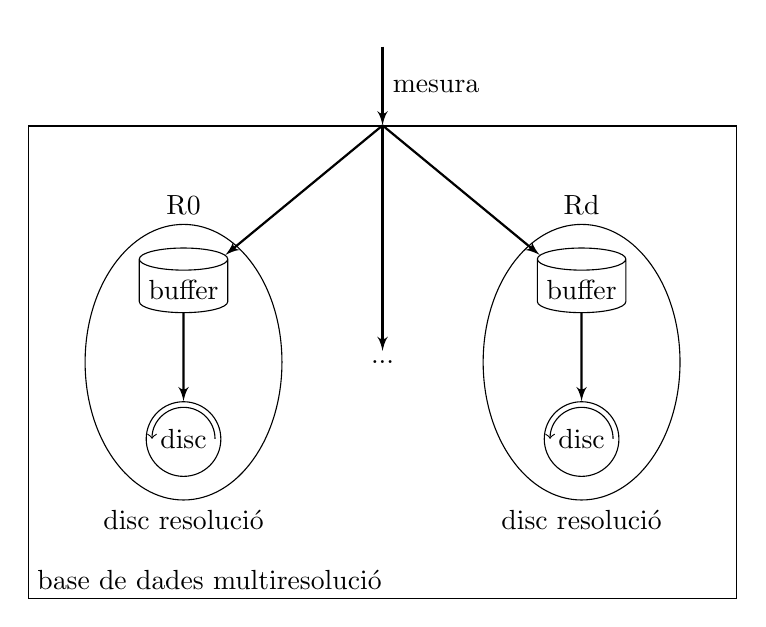
\begin{tikzpicture}
 \tikzset{
        myarrow/.style={->, >=latex',  thick},
      }
      

  \node[rectangle,draw,minimum height=6cm,minimum width=9cm] (m) {};
  \draw[shift=( m.south west)]   
  node[above right] {base de dades multiresolució};


  %discmig
  \node (m.center) (discr1) {...};

  %discr
  
  \node[ellipse,draw,minimum height=3.5cm,minimum width=2.5cm,alias=discr0] [left=of discr1] {};
  \node[above=0cm of discr0.north] {R0};
  \node[below=0cm of discr0] {disc resolució};

  \node[cylinder, draw, shape border rotate=90, aspect=0.25,alias=buffer0] [below=3mm of discr0.north] {buffer};
  \node[circle, draw,alias=disc0]  [above=3mm of discr0.south] {disc} ;
  \draw [->] (disc0.center)++(.4:.4cm) arc(0:180:.4cm);
  \draw[myarrow] (buffer0.bottom) -- (disc0.north);


  %discrd

  \node[ellipse,draw,minimum height=3.5cm,minimum width=2.5cm,alias=discrd] [right=of discr1] {};
  \node[above=0cm of discrd] {Rd};
  \node[below=0cm of discrd] {disc resolució};

  \node[cylinder, draw, shape border rotate=90, aspect=0.25,alias=bufferd] [below=3mm of discrd.north] {buffer};
  \node[circle, draw,alias=discd]  [above=3mm of discrd.south] {disc} ;
  \draw [->] (discd.center)++(.4:.4cm) arc(0:180:.4cm);
  \draw[myarrow] (bufferd.bottom) -- (discd.north);



  %mesura 
  \node[above=1cm of m.north] (m0) {};

  \draw[myarrow] (m0) -- (m.north) 
  node[right,midway] {mesura};

  \draw[myarrow] (m.north) -- (buffer0);
  \draw[myarrow] (m.north) -- (bufferd);
  \draw[myarrow] (m.north) -- (discr1);

\end{tikzpicture}
\caption{Arquitectura d'una BDSTM}
\label{fig:model:bdstm}
\end{figure}


Aquests objectes també permeten definir l'arquitectura d'una BDSTM com
es pot veure a la \autoref{fig:model:bdstm}.  Un SGSTM és una solució
d'emmagatzematge per a sèries temporals a on, resumint, la informació
es distribueix mitjançant diferents resolucions temporals.  Una sèrie
temporal multiresolució és una co\l.lecció de subsèries resolució, les
quals acumulen temporalment mesures en un buffer a on són processades
i finalment emmagatzemades en un disc. El processament de les dades té
per objectiu canviar els intervals de temps entre les mesures per tal
de compactar la informació de les sèries temporals. D'aquesta manera,
les sèries temporals queden emmagatzemades en diferents resolucions
temporals distribuïdes en els discs.

Els discs tenen la mida limitada i només poden contenir un nombre
fixat de mesures. Quan un disc no té més capacitat ha d'eliminar una
mesura. Com a conseqüència una BDSTM té la mida fixada i les sèries
temporals hi queden emmagatzemades a trossos; és a dir com a subsèries
temporals. 


En aquesta secció només es defineixen els conceptes referents a
l'estructura del model. Aquesta estructura, però, requereix uns
operadors específics per a emmagatzemar-hi i consolidar-hi les
mesures, els quals es defineixen a
l'apartat~\ref{sec:model:sgstm-estructurals}. També requereix unes
funcions per a agregar els atributs de les sèries temporals, els quals
es defineixen a l'apartat~\ref{sec:model:agregador}.




\subsection{Buffer}\label{sec:model:buffer}\todo{falta parlar de regularitat de ST}\todo{falta parlar de representació de ST}
\todo{que quedi clar que els buffers deleguen el càlcul a les $f$}

Un buffer és un contenidor d'una sèrie temporal, regular o no regular, que mitjançant una funció permet regularitzar aquesta sèrie temporal amb un període de mostreig constant. A l'acció de regularitzar un interval d'una sèrie temporal l'anomenarem consolidació, al període de mostreig contant l'anomenarem pas de consolidació i a la funció de regularització l'anomenarem agregador d'atributs.

\begin{definition}[Buffer]
  Definim \emph{buffer} com el tuple
  \glsdispdef{not:buffer}{$(S,\tau,\delta,f)$}, en el que
  \glsdispdef{not:sgstm:sb}{$S$} és una sèrie temporal,
  \glsdispdef{not:sgstm:tau}{$\tau$} és el darrer instant de temps de
  consolidació, \glsdispdef{not:sgstm:delta}{$\delta$} és la durada
  del pas de consolidació i \glsdispdef{not:sgstm:f}{$f$} és un
  agregador d'atributs.
\end{definition}

La consolidació d'una sèrie temporal s'inicia en un instant de temps
concret i té lloc a cada pas de consolidació. Amb la finalitat
d'establir els intervals de consolidació de la sèrie temporal, es
defineix un buffer inicial.

\begin{definition}\label{def:model:buffer_buit}
  Definim buffer inicial o buffer buit com el buffer $B_{\emptyset} =
  (\emptyset,t_0, \delta_0, f)$, el qual
  conté una sèrie temporal buida, l'instant de temps inicial de
  consolidació, una durada que indica el pas de consolidació i un
  agregador d'atributs.
\end{definition}

A partir del buffer buit es poden conèixer tots els instants de temps
de consolidació del buffer, els quals seran $t_0+k\delta,
k\in\mathbb{N}$. Aquests instants de temps de consolidació també
defineixen els intervals de temps de consolidació del buffer de la
forma $i=[\tau,\tau+\delta]$. La consolidació de la sèrie temporal $S$
d'un buffer en un interval de temps $i$ dóna com a resultat una mesura
$m=(t,v)$ calculada a partir de l'agregador d'atributs $m = f (S,
i)$. Més endavant a la \autoref{sec:model:agregador} detallem el
concepte d'agregador d'atributs.








\subsection{Disc}\label{sec:model:disc}

Un disc és un contenidor d'una sèrie temporal regular amb un nombre
acotat de mesures. En arribar al nombre màxim de mesures permeses,
cada cop que s'afegeix una mesura nova s'elimina la mesura mínima de
la sèrie temporal.  Així doncs, un disc és semblant a una cua
\emph{First In First Out} (FIFO), a on el primer d'arribar és el
primer de sortir.

\begin{definition}[Disc]
  Definim \emph{disc} com el tuple \glsdispdef{not:disc}{$(S,k)$}, en
  el que \glsdispdef{not:sgstm:sd}{$S$} és una sèrie temporal i
  \glsdispdef{not:sgstm:k}{$k\in\N{}$} és el cardinal màxim de $S$.
\end{definition}

A l'inici, un disc no conté mesures però cal que estigui caracteritzat
pel cardinal màxim. Amb aquesta finalitat es defineix un disc inicial.

\begin{definition}\label{def:model:disc_buit}
  Definim disc inicial o disc buit com el disc $D_{\emptyset} =
  (\emptyset,k)$, el qual conté una sèrie temporal buida i el cardinal
  màxim que podrà prendre $S$.
\end{definition}




\subsection{Subsèrie resolució}\label{sec:model:subserie-resolucio}

Una subsèrie temporal resolució és una parella de disc i buffer. En el
buffer hi ha la part d'una sèrie temporal a regularitzar i en el disc
hi ha l'altra part ja regularitzada, amb un nombre acotat de
mesures. A l'acció de regularitzar l'anomenem consolidar en coherència
amb el concepte descrit pels buffers.


\begin{definition}[Subsèrie resolució]
  Definim \emph{subsèrie resolució} com el tuple
  \glsdispdef{not:subserieresolucio}{$(B,D)$}, en el que $B$ és un buffer i $D$
  és un disc.
\end{definition}
 
La definició de buffer buit (def.~\ref{def:model:buffer_buit}) i de
disc buit (def.~\ref{def:model:disc_buit}) indueixen a una definició
de subsèrie resolució buida.
\begin{definition}\label{def:model:subserie_resolucio_buida}
  Definim subsèrie resolució buida com la subsèrie resolució $R_{\emptyset}
  = (B_{\emptyset},D_{\emptyset})$, la qual conté un buffer buit i un
  disc buit.
\end{definition}


Les subsèries resolució es consoliden seguint els criteris del seu
buffer i emmagatzemant la mesura de consolidació al seu disc.




\subsection{Sèrie temporal multiresolució}

Una sèrie temporal multiresolució és un conjunt de subsèries resolució que
comparteixen l'entrada de mesures, les quals provenen d'una mateixa
sèrie temporal. La sèrie temporal queda regularitzada i distribuïda en
les diferents subsèries resolució amb resolucions diferents, tal com s'ha
vist a la \autoref{fig:model:bdstm}


\begin{definition}[Sèrie temporal multiresolució]
  Definim \emph{sèrie temporal multiresolució} com el conjunt de subsèries
  resolució \glsdispdef{not:seriemultiresolucio}{$M=\{R_0,\dotsc,R_d\}$}.
\end{definition}

A partir de la definició de subsèrie resolució buida
(def.~\ref{def:model:subserie_resolucio_buida}) és defineix la sèrie
temporal multiresolució buida.
 
\begin{definition}\label{def:model:st_multiresolucio_buit}
  Definim sèrie temporal multiresolució buida com el conjunt de subsèries
  resolució buides
  $M_{\emptyset}=\{R_{0_{\emptyset}},\dotsc,R_{d_{\emptyset}\}}$.
\end{definition}

Normalment, en una sèrie temporal multiresolució no hi ha dues subsèries
resolució amb la mateixa informació. És a dir, donats dues subsèries
resolució $R_a = (B_a, D_a)$ i $R_b = (B_b, D_b)$, els seus respectius
buffers $B_a=(S_a,\tau_a,\delta_a,f_a)$ i
$B_b=(S_b,\tau_b,\delta_b,f_b)$ no tenen el mateix interval de
consolidació i agregador d'atributs: $\delta_a \neq \delta_b \wedge
f_a \neq f_b$.




\subsection{Base de dades de sèries temporals
  multiresolució}\label{sec:model:bdstm}

Una base de dades de sèries temporals multiresolució (BDSTM) és una
co\l.lecció de sèries temporal multiresolució.  Les sèries temporals
es poden emmagatzemar exclusivament en una BDSTM o poden conviure amb
altres tipus de dades en bases de dades que tinguin capacitats de
BDSTM.


Una BDSTM té uns paràmetres que cal configurar per a cada sèrie
temporal multiresolució: pas de consolidació, funció d'agregació,
etc. Anomenem esquema de multiresolució a l'efecte que produeixen les
configuracions possibles d'aquests paràmetres. Així doncs, a cada
BDSTM li podem observar i manipular els seus esquemes de
multiresolució, el qual mostrem amb més detall a
l'apartat~\ref{sec:model:sgstm-manipulacio-esquema}.



\subsubsection{Relació sèrie temporal multiresolució}


Una sèrie temporal multiresolució és una relació de buffers i discs. A
cada parella buffer-disc l'anomenem subsèrie resolució. Així doncs, una
sèrie temporal multiresolució és un conjunt de subsèries resolució.

Com a conjunt de subsèries resolució, una sèrie temporal multiresolució
s'observa com una relació de grau sis a on la capçalera conté els
atributs
\begin{itemize}
\item sèrie temporal del buffer ($S_B$),
\item sèrie temporal del disc ($S_D$),
\item darrer instant de consolidació ($\tau$),
\item pas de consolidació ($\delta$),
\item màxim cardinal del disc ($k$),
\item i funció d'agregació d'atributs ($f$).
\end{itemize}

Una restricció habitual és que $\delta$ i $f$ no estiguin repetits; és
a dir que ($\delta$,$f$) són els atributs clau de la relació sèrie
temporal multiresolució.

Així doncs observada com a relació, tal com s'ha fet en el model de
SGST, podem escriure una sèrie temporal multiresolució
\begin{definition}[Representació sèrie temporal multiresolució]
  Sigui $M=\{R_0,\dotsc,R_d\}$ una sèrie temporal multiresolució a on
  $R_i =(B_i,D_i)$ són subsèries resolució amb domini de sèrie
  temporal per les sèries temporals, de $\bar{\R{}}$ pels temps, de
  $\N{}$ pel pas de consolidació i de funció per a la funció
  d'agregació d'atributs;
  \glsdispdef{not:sgstm:relaciomultiresolucio}{representada com a relació}
  s'escriu com $ M = ( S_B: \text{Sèrie Temporal}, S_D: \text{Sèrie
    Temporal}, \tau: \R{}, \delta: \R{}, k: \N{}, f: \text{funció}\},
  \{ \{ S_B: S_{B_0} , S_D : S_{D_0} , \tau : \tau_{B_0}, \delta :
  \delta_{B_0}, k: k_{D_0}, f : f_{B_0} \} , \dotsc, \{ S_B: S_{B_d} ,
  S_D : S_{D_d} , \tau : \tau_{B_d}, \delta : \delta_{B_d}, k:
  k_{D_d}, f : f_{B_d} \} \} )$.
\end{definition}

De la mateixa manera que per a les sèries temporals en el model de
SGST, una sèrie temporal multiresolució es pot escriure de manera
simplificada com al conjunt de tuples $M = \{ (S_{B_0}, S_{D_0} ,
\tau_{B_0}, \delta_{B_0}, k_{D_0}, f_{B_0} ), \dotsc, (S_{B_d},
S_{D_d} , \tau_{B_d}, \delta_{B_d}, k_{D_d}, f_{B_d} ) \}$.




\subsection{Exemples}

\begin{example} [Sèrie temporal multiresolució]
\label{ex:model:bdm1}%ATENCIÓ als canvis: les dades d'aquest exemple s'utilitzen en altres apartat.


Sèrie temporal multiresolució $M_1=\{R_0,R_1\}$ que té dues subsèries
resolució amb els paràmetres següents:
\begin{itemize}
\item La subsèrie resolució $R_0$ té un pas de consolidació de 5
  unitats de temps, una mida màxima de 4 mesures i una funció de
  consolidació de 'mitjana' de les mesures.
\item La subsèrie resolució $R_1$ té un pas de consolidació de 10
  unitats de temps, una mida màxima de 3 mesures i una funció de
  consolidació de 'mitjana' de les mesures.
\end{itemize}

\begin{figure}[tp]
\centering
%\usetikzlibrary{shapes,arrows,positioning}
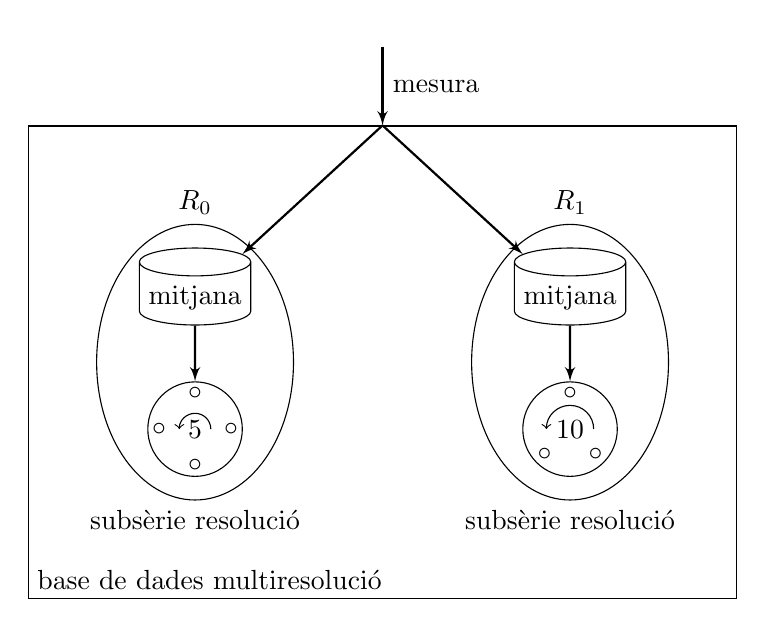
\begin{tikzpicture}
 \tikzset{
        myarrow/.style={->, >=latex',  thick},
      }
      

  \node[rectangle,draw,minimum height=6cm,minimum width=9cm] (m) {};
  \draw[shift=( m.south west)]   
  node[above right] {base de dades multiresolució};


  %discmig
  \node (m.center) (discr1) {};

  %discr
  
  \node[ellipse,draw,minimum height=3.5cm,minimum width=2.5cm,alias=discr0] [left=of discr1] {};
  \node[above=0cm of discr0.north] {$R_0$};
  \node[below=0cm of discr0] {subsèrie resolució};

  \node[cylinder, draw, shape border rotate=90, aspect=0.25,alias=buffer0] [below=3mm of discr0.north] {mitjana};
  \node[circle, draw,alias=disc0,minimum width=1.2cm]  [above=3mm of discr0.south] {5} ;
  \draw [->] (disc0.center)++(.2:.2cm) arc(0:180:.2cm);
  \draw[myarrow] (buffer0.bottom) -- (disc0.north);

  \node[circle,minimum width=9mm] (d0boles) [below=0mm of disc0.center,anchor=center] {};
  \node[below=0mm of d0boles.north,anchor=center] {$\circ$};
  \node[below=0mm of d0boles.east,anchor=center] {$\circ$};
  \node[below=0mm of d0boles.south,anchor=center] {$\circ$};
  \node[below=0mm of d0boles.west,anchor=center] {$\circ$};


  %discrd

  \node[ellipse,draw,minimum height=3.5cm,minimum width=2.5cm,alias=discrd] [right=of discr1] {};
  \node[above=0cm of discrd] {$R_1$};
  \node[below=0cm of discrd] {subsèrie resolució};

  \node[cylinder, draw, shape border rotate=90, aspect=0.25,alias=bufferd] [below=3mm of discrd.north] {mitjana};
  \node[circle, draw,alias=discd,minimum width=1.2cm]  [above=3mm of discrd.south] {10} ;
  \draw [->] (discd.center)++(.3:.3cm) arc(0:180:.3cm);
  \draw[myarrow] (bufferd.bottom) -- (discd.north);

  \node[circle,minimum width=9mm] (d1boles) [below=0mm of discd.center,anchor=center] {};
  \node[below=0mm of d1boles.north,anchor=center] {$\circ$};
  \node[below=0mm of d1boles.south east,anchor=center] {$\circ$};
  \node[below=0mm of d1boles.south west,anchor=center] {$\circ$};


  %mesura 
  \node[above=1cm of m.north] (m0) {};

  \draw[myarrow] (m0) -- (m.north) 
  node[right,midway] {mesura};

  \draw[myarrow] (m.north) -- (buffer0);
  \draw[myarrow] (m.north) -- (bufferd);


\end{tikzpicture}
\caption{Arquitectura de SGSTM particular per l'\autoref{ex:model:bdm1}}
\label{fig:model:ex1}
\end{figure}

L'arquitectura de la base de dades que conté aquesta sèrie temporal
multiresolució es pot veure a la \autoref{fig:model:ex1}. 
 L'esquema
de multiresolució que correspon als instants de consolidació, des de 0
fins a 30, és el següent:
\begin{itemize}
\item La subsèrie resolució $R_0$ serà consolidada en els instants 5,
  10, 15, 20, 25 i 30.
\item La subsèrie resolució $R_1$ serà consolidada en els instants 10,
  20 i 30.
\end{itemize}


Iniciem la base de dades a l'instant de temps 0, instant en el qual la
sèrie temporal multiresolució és $M_1^0 = \{ ( \{\} , \{\} , 0 , 5 ,4
, \text{mitjana} ) , ( \{\} , \{\} , 0 , 10 ,3 , \text{mitjana} ) \}$;
és a dir amb les sèries temporals buides i els darrers instants de
consolidació iniciats a 0.




A continuació, afegim a la sèrie temporal multiresolució les mesures
de la sèrie temporal $S_1=\{
(1,0),(5,0),(8,0),(10,0),(14,0),(19,0),(22,0),(26,0),(29,0) \}$. Tots
els valors valen zero per tal de centrar la comprensió de l'exemple en
l'estructura de temps de consolidació; pel que fa a exemples
d'agregació de valors es poden veure amb més detall a la
secció~\ref{sec:model:agregador}.


Si consolidem la sèrie temporal multiresolució cada cop que sigui
consolidable, és a dir en els instants que marca l'esquema de
multiresolució, a l'instant 29 després d'haver inserit la darrera
mesura la sèrie temporal multiresolució és $M_1^{29} = \{ (
\{(26,0),(29,0)\},\{(10,0),(15,0),(20,0),(25,0)\}, 25 , 5 ,4 ,
\text{mitjana} ), ( \{(22,0),(26,0),(29,0)\}, \{(10,0),(20,0)\},
20 , 10 ,3 , \text{mitjana} ) \}$.  Aquesta sèrie temporal
multiresolució es mostra a la \autoref{fig:model:stm} en forma de
taula.


Es pot observar que als buffers hi ha emmagatzemades les mesures
pendents de consolidar per a cada subsèrie i als discs les darreres
mesures consolidades:
\begin{itemize}
\item Per a la subsèrie resolució $R_0$ hi ha pendent de consolidar
  l'interval de temps $[25,30]$ i al disc hi ha emmagatzemades les 4
  mesures màximes permeses; és a dir que la que s'havia consolidat a
  l'instant $5$ ja s'ha perdut.
\item Per a la subsèrie resolució $R_1$ hi ha pendent de consolidar
  l'interval de temps $[20,30]$ i al disc hi ha emmagatzemades 2
  mesures. El disc encara no ha arribat al cardinal màxim $k=3$ degut
  a que la base de dades s'ha iniciat a l'instant $0$ i la primera
  consolidació d'aquesta subsèrie ha estat a l'instant $10$.
\end{itemize}




\begin{figure}[tp]
  \centering
  \begin{tabular}{|c|c|c|c|c|c|}
    \multicolumn{2}{c}{$M_1^{29}$} \\ \hline
    $S_B$  & $S_D$ & $\tau$ & $\delta$ & $k$ & $f$ \\ \hline
      \begin{tabular}{|c|c|}
         \hline
         $t$  & $v$ \\ \hline
         26  & 0 \\
         29 & 0 \\\hline
       \end{tabular} & 
      \begin{tabular}{|c|c|}
         \hline
         $t$  & $v$ \\ \hline
         10  & 0 \\
         15  & 0 \\
         20 & 0 \\ 
         25 & 0 \\\hline
       \end{tabular} 
       & 25 & 5  & 4 & mitjana  \\ \hline
       \begin{tabular}{|c|c|}
         \hline
         $t$  & $v$ \\ \hline
         22  & 0 \\
         26  & 0 \\
         29 & 0 \\\hline
       \end{tabular} & 
      \begin{tabular}{|c|c|}
         \hline
         $t$  & $v$ \\ \hline
         10  & 0 \\
         20  & 0 \\\hline
       \end{tabular}  
       & 20 & 10 & 3 & mitjana  \\ \hline
  \end{tabular}
  \caption{Taula d'una sèrie temporal multiresolució}
  \label{fig:model:stm}
\end{figure}

\end{example}


\begin{example} [Sèrie temporal multiresolució amb vistes]

  En el model relacional de SGBD molt sovint s'utilitzen vistes per a
  agrupar informació de vàries relacions, per a mostrar-ne una part,
  etc. Una vista és una variable relació virtual derivada d'una
  expressió relacional \parencite{date13}. En aquest exemple mostrem
  la mateixa sèrie temporal multiresolució de
  l'\autoref{ex:model:bdm1} però organitzada amb forma de vistes
  relacionals.


  Sigui $M_2^{\text{series}}= ((S':\text{nom},S:\text{sèrie
    temporal}),\{ (S_{B1},\{(26,0),(29,0)\}),
  (S_{B2},\{(22,0),(26,0),(29,0)\}),
  (S_{D1},\{(10,0),(15,0),(20,0),(25,0)\}),
  (S_{D2},\{(10,0),(20,0)\} )\})$ una relació de sèries
  temporals i noms, i $M_2'=
  ((S'_B:\text{nom},S'_D:\text{nom},\tau:\R,\delta:\R,k:\N,f:\text{funció}
  ),\{ (S_{B1},S_{D1},25 ,5 ,4 ,\text{mitjana} ), ( S_{B2},S_{D2},20 ,
  10 ,3 , \text{mitjana} ) \})$ una sèrie temporal multiresolució amb
  noms als atributs de sèries temporals; la vista de la sèrie temporal
  multiresolució es mostra a la \autoref{fig:model:stm:vistes} i es
  defineix com a
  \begin{align*}
    \text{vista } M_2 =& (M_2' \join ( M_2^{\text{series}} \rename S' \as S_B', S \as S_B )) \\
    &\join ( M_2^{\text{series}} \rename S' \as S_D', S \as S_D )
    \{\text{all but } S_B',S_D' \}
  \end{align*}




  \begin{figure}[tp]
    \centering
    \begin{tabular}{|c|c|c|c|c|c|}
      \multicolumn{2}{c}{$M'_2$} \\ \hline
      $S'_B$  & $S'_D$ & $\tau$ & $\delta$ & $k$ & $f$ \\ \hline
      $S_{B1}$ & $S_{D1}$ & 25 & 5  & 4 & mitjana  \\
      $S_{B2}$ & $S_{D2}$ & 20 & 10 & 3 & mitjana  \\ \hline
    \end{tabular}\qquad
    \begin{tabular}{|c|c|c|}
      \multicolumn{3}{c}{$M^{\text{series}}_{2}$} \\ \hline
      \multirow{2}{*}{$S'$}  &  \multicolumn{2}{c|}{$S$} \\ \cline{2-3}
      & $t$      & $v$  \\ \hline
      \multirow{2}{*}{$S_{B1}$} 
      & 26 & 0 \\ 
      & 29 & 0 \\ \hline
      \multirow{3}{*}{$S_{B2}$} 
      & 22 & 0 \\ 
      & 26 & 0 \\ 
      & 29 & 0 \\ \hline
      \multirow{4}{*}{$S_{D1}$} 
      & 10 & 0 \\ 
      & 15 & 0 \\ 
      & 20 & 0 \\ 
      & 25 & 0 \\ \hline
      \multirow{2}{*}{$S_{D2}$} 
      & 10 & 0 \\ 
      & 20 & 0 \\ \hline
    \end{tabular}
    \caption{Taula d'una sèrie temporal multiresolució amb vistes
      relacionals}
    \label{fig:model:stm:vistes}
  \end{figure}


  D'aquesta manera $M_2$ té els mateixos valors que la $M_1$ definida
  a l'exemple anterior; observant només el resultat de $M_2$ no es pot
  distingir que és una vista. Així doncs, les vistes ens permeten
  organitzar una sèrie temporal multiresolució de forma més còmoda i,
  a més tal com es descriu a \textcite{date13}, mantenint que totes
  les operacions i propietats que són d'aplicació a les relacions ho
  són també a les seves vistes.


%S'observa que per tal de complir amb les propietats de les relacions, totes les sèries temporals dels buffers han de ser del mateix tipus, és a dir tenir la mateixa capçalera. El mateix succeeix amb les sèries temporals dels discs. (Vegeu els exemples de la secció \ref{par:model:exemple-relvalues} sobre valors relació). No obstant les mesures que entren a la base de dades provenen de la mateixa sèrie temporal i per tant les sèries temporals emmagatzemades sempre seran del mateix tipus.



\end{example}



\begin{example} [Sèrie temporal multiresolució amb desfasaments]
\label{ex:model:bdm-desfasaments}

A l'\autoref{ex:model:bdm1} s'ha mostrat una sèrie temporal
multiresolució en la que la consolidació de les dues subsèries obeeix
a la mateixa funció d'agregador d'atributs $f$. En aquest exemple
treballem amb els mateixos valors que a l'\autoref{ex:model:bdm1} però
ara canviem la funció de la segona subsèrie resolució per un agregador
amb desfasament; és a dir que cada cop que consolida retorna una
mesura amb un retard d'una certa durada. Aquest nou agregador que
anomenem \emph{mitjanad5} també fa la mitjana però amb un desfasament
de $5$ unitat de temps, a l'apartat
\ref{sec:model:sgstm-manipulacio-esquema} es defineix amb més precisió
aquest concepte de desfasament.


Seguint el mateix procediment que a l'\autoref{ex:model:bdm1}, a
l'instant 29 després d'haver inserit la darrera mesura la sèrie
temporal multiresolució és $M_3^{29} = \{ ( \{(26,0),(29,0)\} ,
\{(10,0),(15,0),(20,0),(25,0)\} , 25 , 5 ,4 , \text{mitjana} ) , (
\{(19,0),(22,0),(26,0),(29,0)\} , \{(5,0),(15,0)\} , 20 , 10 ,3 ,
\text{mitjanad5} ) \}$.  Aquesta sèrie temporal multiresolució es
mostra a la \autoref{fig:model:stm:desfasaments} en forma de taula.


\begin{figure}[tp]
  \centering
  \begin{tabular}{|c|c|c|c|c|c|}
    \multicolumn{2}{c}{$M_3^{29}$} \\ \hline
    $S_B$  & $S_D$ & $\tau$ & $\delta$ & $k$ & $f$ \\ \hline
      \begin{tabular}{|c|c|}
         \hline
         $t$  & $v$ \\ \hline
         26  & 0 \\
         29 & 0 \\\hline
       \end{tabular} & 
      \begin{tabular}{|c|c|}
         \hline
         $t$  & $v$ \\ \hline
         10  & 0 \\
         15  & 0 \\
         20 & 0 \\ 
         25 & 0 \\\hline
       \end{tabular} 
       & 25 & 5  & 4 & mitjana  \\ \hline
       \begin{tabular}{|c|c|}
         \hline
         $t$  & $v$ \\ \hline
         19  & 0 \\
         22  & 0 \\
         26  & 0 \\
         29 & 0 \\\hline
       \end{tabular} & 
      \begin{tabular}{|c|c|}
         \hline
         $t$  & $v$ \\ \hline
          5  & 0 \\
         15  & 0 \\\hline
       \end{tabular}  
       & 20 & 10 & 3 & mitjanad5  \\ \hline
  \end{tabular}
  \caption{Taula d'una sèrie temporal multiresolució amb desfasaments}
  \label{fig:model:stm:desfasaments}
\end{figure}



Així doncs, mentre que l'esquema de multiresolució segueix sent el
mateix pel que fa als instants de consolidació, els instants de temps
de la sèrie temporal emmagatzemada a la subsèrie resolució $R_1$ tenen
un retard de $5$ unitats de temps.  Per una banda, es pot observar a
la $S_{B2}$ que el buffer ara és 5 unitats més gran i emmagatzema
mesures de l'interval $[15,30]$. Per altra banda, es pot observar a la
$S_{D2}$ que els instants emmagatzemats són $5$ i $15$ corresponents
als instants de consolidació $10$ i $20$. Pel que fa a la resta de
valors, no han variat respecte de l'\autoref{ex:model:bdm1}.



\end{example}


%%% Local Variables: 
%%% mode: latex
%%% TeX-master: "main"
%%% End: 

% LocalWords:  buffers multiresolució agregador l'agregador subsèries
% LocalWords:  d'agregador

\section{Model d'operacions}

En aquesta secció es defineixen els operadors que permeten modelar el
comportament i la manipulació de les dades en el model de SGSTM.

Per a treballar amb les sèries temporals multiresolució s'utilitzen
els conceptes descrits al model d'operacions de SGST. El model de
SGSTM es defineix a partir del model de SGST i per tant les operacions
dels SGSTM també hi estan basades. Tot i així cal tenir en compte dues
particularitats.

Per una banda, el model de SGSTM treballa amb sèries temporals
multiresolució. Així, es defineixen operadors que permeten extreure
les sèries temporals emmagatzemades en aquestes bases de dades amb
l'objectiu d'aplicar-hi posteriorment els operadors dels SGST.

Per altra banda, el model de SGSTM té una estructura específica que
requereix ser manipulada coherentment. Així, es defineixen operadors
que saben treballar amb aquesta estructura agrupats en dos grups.  El
primer grup són els operadors requerits pel model estructural;
operadors que són inseparables de l'estructura i són utilitzats en el
procés d'emmagatzemar les mesures. El segon grup són els operadors
necessaris per a manipular l'estructura; és a dir operadors que
permeten fer canvis en l'esquema de la base de dades o consultar
paràmetres de l'esquema actual.


En el disseny del model d'operacions següent es distingeixen tres
grups d'operadors segons els casos anteriors:

\begin{itemize}
\item Estructurals: operadors requerits pel model estructural.
\item Manipulació de l'esquema: operadors per a manipular l'esquema de
  multiresolució.
\item Consultes: operadors per a extreure les sèries temporals
  emmagatzemades.
\end{itemize}





\subsection{Estructurals}
\label{sec:model:sgstm-estructurals}

En el model estructural de SGSTM hem definit les sèries temporals
multiresolució com un conjunt de subsèries resolució a les quals es
van afegint mesures compactant-les i consolidant-les. En aquest
apartat definim els operadors que permeten inserir mesures noves i
consolidar-les al seu lloc corresponent en l'estructura.

A continuació es descriuen els operadors associats a cada objecte del
model de SGSTM.


\subsubsection{Buffer}

Els buffers reben les noves mesures i les consoliden a cada instant de
consolidació. Així, tenen dos operadors associats: un per afegir noves
mesures al buffer i un altre per consolidar-les.


L'operació d'afegir una mesura al buffer consisteix en afegir-la a la
sèrie temporal pendent de consolidar.
\begin{definition}[Afegeix mesura al buffer]
  Sigui $B=(S,\tau,\delta,f)$ un buffer i $m=(t,v)$ una mesura, la
  inserció de la mesura al buffer $\addB(B,m)$ és un buffer
  $B'=(S',\tau,\delta,f)$ amb la mesura afegida a la sèrie temporal
  del buffer: $\addB(B,m) = (S',\tau,\delta,f)$ a on $S'=S\cup \{m\}$.
\end{definition}


L'operació de consolidació d'un buffer consisteix en compactar les
mesures segons els intervals de consolidació i la funció d'agregació i
a suprimir la part ja consolidada de la sèrie temporal.  Així doncs,
la consolidació d'un buffer per cada interval de temps
$i=[\tau,\tau+\delta]$ dóna com a resultat una mesura calculada en
funció de l'agregador d'atributs i un nou buffer amb la sèrie temporal
reduïda.
\begin{definition}[Consolida el buffer]
  Sigui $B=(S,\tau,\delta,f)$ un buffer, la consolidació del buffer
  $\consB(B)$ en l'interval de temps $[\tau,\tau+\delta]$ és un
  buffer $B'=(S',\tau',\delta,f)$, amb el nou instant de consolidació,
  i la mesura $m'=(t',v')$ resultant de la consolidació: $\consB(B) =
  (S',\tau+\delta',\delta,f) \times m'$ a on
  $m'=f(S,[\tau,\tau+\delta])$ i $S'$ és el resultat d'eliminar les
  dades històriques que no es necessiten més. 

  \emph{Nota}: En el model teòric es pot donar $S'=S$ tot i que a les
  implementacions normalment caldrà eliminar les dades ja no
  necessàries per no ocupar espai amb per exemple $S'=
  S[\tau+\delta,+\infty]$.
\end{definition}

De manera simplificada, hem definit que cada consolidació només
s'aplica a l'interval de consolidació actual; així la consolidació
total del buffer és l'aplicació successiva de l'operació de
consolidació.

Aquesta consolidació successiva requereix que les mesures s'insereixen
al buffer ordenades en el temps, sinó un cop duta a terme la
consolidació les mesures inserides desordenades poden no ser tingudes
en compte. Si es duu a terme aquesta inserció ordenada, aleshores un
buffer té l'estat de consolidable quan el temps d'una mesura de la
sèrie temporal és més gran que el següent instant de temps de
consolidació del buffer.
\begin{definition}[Buffer consolidable]\label{def:model:buffer_consolidable}
  Sigui $B=(S,\tau,\delta,f)$ un buffer, definim que $B$ és
  consolidable si i només si $T(m) \geq \tau+\delta$ a on $m=\sup(S)$
  és la mesura suprema de la sèrie temporal del buffer.
\end{definition}



\subsubsection{Disc}

Els discs reben les mesures consolidades per a emmagatzemar-les de
forma acotada. Així, tenen un operador associat que afegeix noves
mesures al disc mantenint sota control el seu cardinal.


L'operació d'afegir una mesura al disc consisteix en afegir-la a la
sèrie temporal i a eliminar la mesura mínima d'aquesta si se supera el
cardinal permès.
\begin{definition}[Afegeix mesura al disc]
  Sigui $D=(S,k)$ un disc i $m=(t,v)$ una mesura, la inserció de la
  mesura al disc $\addD(D,m)$ és un disc $D'=(S',k)$ amb la mesura
  afegida a la sèrie temporal del disc mantenint el cardinal màxim:
  $\addD(S,m) = (S',k)$ a on $S'=
  \begin{cases}
      S\cup\{m\} &\text{si }  |S|<k\\
      (S-\{\min(S)\}) \cup \{m\} &\text{altrament}
    \end{cases}$.
\end{definition}




\subsubsection{Subsèrie resolució}

Les subsèries resolució són l'aparellament d'un buffer amb un disc.
Així tenen dos operadors associats, els quals treballen amb els
operadors del buffer i del disc : un per afegir una mesura al buffer i
un altre per consolidar el buffer i afegir la mesura resultant al disc


L'operació d'afegir una mesura a la subsèrie resolució consisteix en
afegir-la al buffer.
\begin{definition}[Afegeix mesura a la subsèrie resolució]
  Sigui $R=(B,D)$ una subsèrie resolució i $m=(t,v)$ una mesura, la
  inserció de la mesura a la subsèrie resolució $\addR(R,m)$ és una
  subsèrie resolució $R'=(B',D)$ amb la mesura afegida al buffer:
  $\addR(R,m) = (B',D)$ a on $B'=\addB=(B,m)$.
\end{definition}


L'operació de consolidar una subsèrie resolució consisteix en calcular
una mesura de consolidació del buffer, en l'interval de consolidació
actual, i desar-la al disc. Una subsèrie resolució és consolidable
quan ho és el seu buffer.
\begin{definition}[Consolida la subsèrie resolució]
  Sigui $R=(B,D)$ una subsèrie resolució, la consolidació de la
  subsèrie resolució $\consR(R)$ és una subsèrie resolució
  $R'=(B',D')$ a on $(B',m') = \consB(B)$ i $D'=\addD(D,m')$.
\end{definition}





\subsubsection{Sèrie temporal multiresolució}

Les sèries temporals multiresolució són un conjunt de subsèries
resolució. Així tenen dos operadors per a treballar globalment amb
totes les subèries que contingui: un per a afegir una mesura a cada
subsèrie i un altre per a consolidar cadascuna de les subsèries.


L'operació d'afegir una mesura a la sèrie temporal multiresolució
consisteix en afegir-la a cadascuna de les subsèries resolució.
\begin{definition}[Afegeix mesura a la sèrie temporal multiresolució]
  Sigui $M=\{R_0,\dotsc,R_d\}$ una sèrie temporal multiresolució i
  $m=(t,v)$ una mesura, la inserció de la mesura a la sèrie temporal
  multiresolució $\addM(M,m)$ és una sèrie temporal multiresolució
  $M'=\{R_0',\dotsc,R_d'\}$ amb la mesura afegida a cada subsèrie
  resolució: $\addM(M,m) = \{ \forall R_i\in M: \addR(R_i,m) \}$.
\end{definition}


L'operació de consolidar una sèrie temporal multiresolució consisteix
en consolidar cadascuna de les subsèries resolució que siguin
consolidables.

\begin{definition}[Consolida la sèrie temporal multiresolució]
  Sigui $M=\{R_0,\dotsc,R_d\}$ una sèrie temporal multiresolució, la
  consolidació de la sèrie temporal multiresolució $\consM(M)$ és una
  sèrie temporal multiresolució $M'=\{R_0',\dotsc,R_d'\}$ que
  consolida les subsèries resolució consolidables:
  \[
  \consM(M) = \big\{ \forall R_i\in M:
  \begin{cases}
    \consR(R_i) & \text{si } R_i \text{ és consolidable} \\
    R_i & \text{altrament}
  \end{cases}\big\}
  \].
\end{definition}





\subsection{Manipulació de l'esquema}

El model de SGSTM associa a cada sèrie temporal un esquema de
multiresolució. En aquest apartat definim els operadors que permeten
consultar i manipular aquest esquema de multiresolució de forma
coherent amb el model de SGSTM.

L'esquema de multiresolució de cada sèrie temporal multiresolució
consisteix en quatre paràmetres variables: el darrer instant de
consolidació ($\tau$), el pas de consolidació ($\delta$), el cardinal
màxim ($k$) i la funció d'agregació d'atributs ($f$).

Així doncs, quan es manipula una base de dades multiresolució cal
conservar o tractar adequadament aquest esquema de multiresolució.  A
continuació es descriuen operadors per a poder estudiar aquest
esquema, operadors per a canviar-lo i operadors per a unir o ajuntar
dos esquemes.



\subsubsection{Propietats de l'esquema}

La configuració dels quatre paràmetres variables de l'esquema de
multiresolució confereix una sèrie de propietats als objectes d'una
base de dades multiresolució. A continuació definim algunes propietats
que es poden estudiar a partir d'un esquema de multiresolució.




Una propietat de l'esquema de multiresolució és el cronograma que se'n deriva. Així, donat un esquema de multiresolució podem dibuixar la situació relativa en el temps que prendran les mesures.
\todo{fer dibuix aclaridor}


\todo{}

  
Els paràmetres $k$, $\delta$ i $f$ d'una subsèrie resolució són fixats
per l'esquema, mentre que el paràmetre $\tau$ és fixat a un valor
inicial i va sent canviat per l'operació de consolidar. Així doncs,
les propietats que impliquin a $\tau$ dependran de l'instant temporal
en que es faci la consulta i les que no l'impliquin seran fixes per a
cada esquema.



La primera propietat que observem és el lapse temporal d'una subsèrie
resolució; és a dir una mesura de la mida temporal que ocupa la
subsèrie temporal emmagatzemada en el seu disc.
\begin{definition}[Lapse de la subsèrie resolució] %angl. span
  Sigui $R=(S_B,S_D,\tau,\delta,k,f)$ una subsèrie resolució, el seu
  lapse $\text{lapseR}(R)$ és una durada de temps $t^d$ que mesura la
  mida de l'interval que ocupa el disc: $\text{lapseR}(R) = k\delta$.
\end{definition}

\todo{} Si definim l'interval del lapse com a $[\tau - k\delta, \tau]$
i l'interval temporal real de la sèrie temporal del disc com a
$[\min(S_D),\max(S_D)]$, aleshores normalment en el cas que $\max(S_D)=\tau$ es compleix que $\min(S_D)=\tau - (k-1)\delta $: fixem-nos que això pot no complir-se (perquè la sèrie temporal no sigui regular, perquè $\tau$ i $\max(S_D)$ no coincideixin, etc.)
 fixem-nos que el lapse pot no coincidir amb
l'interval temporal real de la sèrie temporal del disc,



Com en diem a la certa variació que es correspon a $t_{actual}-\tau$?





Així doncs podem dir que un disc resolució ens cobreix un span temporal de  $\text{duradaR}(R)$. Es posiciona absolutament des de $\tau$ enrere (si no hi ha iffset). Això vol dir que tindrem un temps recent no cobert de $t_{actual}-\tau$ (anomenar-lo desfasament o retard, en angl. offset), el qual habitualment com a màxim serà de $\delta$ ($t_{actual}-\tau \leq \delta$) i com a mínim de zero si consolidem la multiresolució periòdicament.






Quin és el període de la sèrie temporal d'un disc?
  \begin{gather*}
    \text{periodeR}: R \longrightarrow \delta':\\
    \delta'=
    \begin{cases}
      \delta_r &\text{si } S_D \text{ regular o temps real amb } \delta_r\\
      \delta &\text{altrament}
    \end{cases}
  \end{gather*}


Quin disc conté més resolució?
  \begin{gather*}
    \text{maxR}: R_1 \times R_2 \longrightarrow R_i' | d_i = \max(d_1,d_2) : \\
    d_1 = periodeR(R_1), d_2 = periodeR(R_1)
  \end{gather*}



\subsubsection{Canvis en l'esquema d'un disc resolució}


Redueix o augmenta la mida d'un disc
  \begin{gather*}
    \text{CanviaK}: R \times k' \longrightarrow R': \\
    R' = (S_B,S'_D,\delta,\tau,k',f) : \\
    k_d = |S_D|:\\
    S'_D = \begin{cases}
      S_D         & \text{si } k' \geq k_d   \\
      treuN(S_D,k_d-k')    & \text{altrament}
    \end{cases}, \\
    treuN: S \times n \mapsto S'=  
    \begin{cases}
      S                & \text{si } n=0   \\
      treuN(S - \{\min(S)\},n-1)  & \text{altrament}
    \end{cases}
\end{gather*}


Redueix o augmenta el pas de consolidació d'un disc (sense canviar la sèrie temporal emmagatzemada; ja s'anirà canviant quan es consolidin noves mesures)
  \begin{gather*}
    \text{Canvia}\delta: R \times \delta' \longrightarrow R': \\
    R' = (S_B,S_D,\delta',\tau,k,f)
  \end{gather*}


Redueix o augmenta alhora el pas de consolidació i la mida d'un disc
  \begin{gather*}
    \text{CanviaK}\delta: R \times k' \times \delta' \longrightarrow R': \\
    R' = (S_B,S_D',\delta',\tau,k',f): \\    
    t = \{ \tau-n\delta' | n\in\mathbb{N},n<k' \} \\
    S_D' = \text{seleccioResolucio}(S_D,t)
  \end{gather*}




Afegeix un multivalor per a emmagatzemar sèries temporals multivaluades
  \begin{gather*}
    \text{afegeixMultivalor}: R \longrightarrow R': \\
    R' = (S'_{B},S'_{D},\delta,\tau,k,f): \\
    S'_{B} = \text{map}(S_B,(t,v)\mapsto(t,v,\infty)), \\
    S'_{D} = \text{map}(S_D,(t,v)\mapsto(t,v,\infty))
  \end{gather*}\todo{s'ha de fer amb extends i les v han de poder tenir nom}




\subsubsection{Canvis en l'esquema d'una sèrie temporal multiresolució}

Aplicació de map a una BDM.
\begin{gather*}
  \text{map}: M \times f \longrightarrow M' = \{ f(R_0), \dotsc, f(R_k) \} :\\
   \text{a on } f: R_a \mapsto R'
 \end{gather*}
 
Aplicació de fold a una BDM
\begin{gather*}
  \text{fold}: M \times M_i \times f \longrightarrow M' :\\
  = f(\dots(f(f(f(M_i,R_0),R_1),R_2)\dots),R_k), \\
   \text{a on } f: M_a \times R_b \mapsto M'
\end{gather*}





\subsubsection{Treball amb dos esquemes}


\paragraph{Unió de multiresolució}

Cas típic:
Mesuro una sèrie temporal. Durant un temps emmagatzemo valors a una
base de dades i després els emmagatzemo a una altra base de dades. Al final vull unir les dues bases de dades.


Unió de dos discs resolució que tenen el mateix $\delta$ i $f$ és un
disc resolució que conté la unió de les sèries de cada un.  Sigui
$R_1^*=(S_{B1},S_{D1},\delta,\tau_1,k_1,f)$ i
$R_2^*=(S_{B2},S_{D2},\delta,\tau_2,k_2,f)$
  \begin{gather*}
    \text{unioR}: R_1^* \times R_2^* \longrightarrow R': \\
    R' = (S'_B,S'_D,\delta,\max(\tau_1,\tau_2),k_1+k_2,f), \\
    S_{Di}, S_{Dj} | R_i = \text{maxR}(R_1,R_2), j \neq i:  \\
    S'_B = \text{unio}(S_{B1},S_{B2})\\
    S'_D = \text{unio}^r(S_{Di},S_{Dj})
\end{gather*}

També es pot unir dos discs resolució amb diferent $\delta$ i $f$,
però llavors s'ha de determinar quins són els $\delta'$ i $f'$
resultants.


Com a relacions multiresolució, dues bases de dades multiresolució es
poden unir si no intersecten en les claus $(\delta,f)$.  En cas que
intersectin, podem definir la unió multiresolució com la unió que sap unir els discs resolució repetits.

\begin{gather*}
    \text{UnioM}: M_1 \times M_2 \longrightarrow M': \\
    K_1 = \{(delta_1,f_1) \in M_1\},K_2 = \{(delta_2,f_2) \in M_2\}, \\
    K_a = K_1 \cap K_2, K_u =  (K_1 \cup K_2) - K_a : \\
    M_{u1}'= seleccio(M_1, (delta,f) \in K_u)\\
    M_{u2}'= seleccio(M_2, (delta,f) \in K_u)\\
    M_a = \{\forall R_1\in M_1,R_2\in M_2: unioR(R_1,R_2) |
       (delta_1,f_1) = (delta_2,f_2) \} \\
    M' =  M_{a} \cup  M'_{1}  \cup  M'_{2}     
\end{gather*}






\paragraph{Junció de multiresolució}

\todo{canviar fusió per junció}

Tinc una sèrie temporal en una base de dades, i una altra sèrie temporal en una altra base de dades. Vull emmagatzemar-les totes dues en una mateixa base de dades amb una sèrie temporal multivaluada.


Fusió de dos discs resolució que tenen el mateix $\delta$ i $f$.
Sigui $R_1^*=(S_{B1},S_{D1},\delta,\tau_1,k_1,f)$ i
$R_2^*=(S_{B2},S_{D2},\delta,\tau_2,k_2,f)$
  \begin{gather*}
    \text{FusioR}: R_1^* \times R_2^* \longrightarrow R': \\
    R' = (S'_B,S'_D,\delta,\max(\tau_1,\tau_2),k_1+k_2,f), \\
    S'_B = \text{fusio}^r(S_{B1},S_{B2})\\
    S'_D = \text{fusio}^r(S_{D1},S_{D2})
\end{gather*}


Fusió de dues bases de dades multiresolució
\begin{gather*}
    \text{FusioM}: M_1 \times M_2 \longrightarrow M': \\
    K_1 = \{(delta_1,f_1) \in M_1\},K_2 = \{(delta_2,f_2) \in M_2\}, \\
    K_a = K_1 \cap K_2, K_u =  (K_1 \cup K_2) - K_a : \\
    M_{u1} =\text{afegeixMultivalor}(seleccio(M_1, (delta,f) \in K_u))\\
    M_{u2} =\text{afegeixMultivalor}^{v0} (seleccio(M_2, (delta,f) \in K_u))\\
    M_1 = seleccio(M_1, (delta,f) \in K_f) \\
    M_2 = seleccio(M_2, (delta,f) \in K_f) \\
    M_a = \{\forall R_1\in M_1,R_2\in M_2: fusioR(R_1,R_2) |
       (delta_1,f_1) = (delta_2,f_2) \} \\
    M' =  M_{a} \cup  M_{u1}  \cup  M_{u2}     
\end{gather*}






\subsection{Consultes}



Operadors per fer consultes sobre una base de dades multiresolució. 

Mostrar com s'utilitzen els operadors dels SGST quan tenim multiresolució.


* Abans de fer una consulta temporal pot fer falta fer una selecció dels discs resolució amb el mateix interpolador.

* Fer una unió temporal de tots els discs de la BDM i treballar sobre aquest senyal $\longrightarrow$ Abstracció d'una BDSTM com a sèrie temporal; és possible treballar amb una BDSTM com si fos una sèrie temporal?

  - Com a consulta total: $\text{SerieTotal}(M)$

  - Com a consulta amb informació multiresolució: $\text{DiscSelecció}(M,\delta,f)$

* Pensar com operar (per exemple sumar) amb sèries temporals de diferents BDM. 




\subsubsection{Selecció de disc}


Consulta la subsèrie de la BDSTM que té una resolució i atribut
determinat. 


\begin{definition}[DiscSelecció]
  \begin{gather*}
    \text{DiscSelecció}: M \times \delta \times f \longrightarrow S' = S_D: \\
    (S_B,S_D,\delta,\tau,k,f) \in M
\end{gather*}
\end{definition}



\subsubsection{Sèrie temporal total}



\begin{definition}[Sèrie temporal total]
  Sigui $M^*$ una base de dades multiresolució a on no hi ha $\delta$ repetits
  \begin{gather*}
    \text{SerieTotal}: M^* \longrightarrow S': \\
    \forall (S_{Bi},S_{Di},\delta_i,\tau_i,k_i,f_i) \in M : \\
    \delta_0 < \delta_1 < \delta_2 < \dots < \delta_d : \\
    S' = S_{D0} || S_{D1} || S_{D2} || \dotsb || S_{Dd}
\end{gather*}
\end{definition}

Prèviament es pot fer una selecció dels discs resolució que
comparteixin un determinat agregador d'atributs. \todo{També hi podria
  haver una operació estructural que sabés fusionar dos discs
  resolució}



L'operació de consulta de la sèrie temporal total també es pot aplicar
tenint en compte la representació.
\begin{definition}[Sèrie total amb representació]
  Sigui $M^*$ una base de dades multiresolució a on no hi ha $\delta$
  repetits i $r$ una representació
  \begin{gather*}
    \text{SerieTotal}: M^* \times r \longrightarrow S': \\
    \forall (S_{Bi},S_{Di},\delta_i,\tau_i,k_i,f_i) \in M : \\
    \delta_0 < \delta_1 < \delta_2 < \dots < \delta_d : \\
    S' = S_{D0} \cup^r S_{D1} \cup^r  S_{D2}  \cup^r \dotsb \cup^r  S_{Dd}
\end{gather*}
\end{definition}



\paragraph{Selecció de resolució}


Per a extreure una resolució determinada de la sèrie temporal
emmagatzemada a la base de dades multiresolució, es consulta la sèrie
temporal total i s'aplica una selecció de resolució
$\text{SerieTotal}(M)[i]^r$ a on $i$ és el conjunt d'instants de
temps.






%%% Local Variables:
%%% TeX-master: "main"
%%% End:
% LocalWords:  SGSTM l'agregador buffer multiresolució subsèries
% LocalWords:  subsèrie


\section{Funcions d'agregació d'atributs}
\label{sec:model:interpolador}
\label{sec:model:agregador}
\glsaddsection{not:sgstm:fdef} %%%%secció de model
\glsaddsection{not:sgstm:f} %%%%secció de model


Les funcions d'agregació d'atributs s'utilitzen en la consolidació
dels buffers per tal de compactar certa informació de la sèrie
temporals. Sigui $S$ una sèrie temporal i $t_a$ i $t_b$ dos instants
de temps, una funció d'agregació d'atributs $f$ calcula una mesura que
resumeix la informació de $S$ en un interval de temps $i=[t_a,t_b]$:
\[
f: \text{sèrie temporal} \glsdisp{not:times}{\times}
\text{interval de temps} \longrightarrow \text{mesura}
\]
\[
f: S=\{m_0,\dotsc,m_k\} \times i=[t_a,t_b] \longrightarrow  m'
\]


Generalment, $m'$ resulta d'aplicar dues operacions a $S$: 
\begin{enumerate}
\item una selecció d'una subsèrie $S'$ segons l'interval de temps $i$,
  per exemple $S' = S[t_a,t_b]$
\item i una agregació en aquesta subsèrie $m' =
  \glssymbol{not:sgst:aggregate}(S',m_i,\glssymbol{not:sgst:fagg})$ on
  $\glssymbol{not:sgst:fagg}$ i $m_i$ són els atributs d'aquesta agregació.
\end{enumerate}



Atès que hi ha maneres diferents de resumir la informació d'una sèrie
temporal, cal plantejar diferents funcions d'agregació d'atributs. Per
exemple, es poden calcular estadístics de la sèrie temporal, com el
valor màxim o la mitjana; aplicar operacions de processament digital
del senyal, com fan \textcite{zhang11}, o algoritmes per a detectar
comportaments aberrants, com fa \textcite{lisa00:brutlag}. A més a
més, la representació de les sèries temporals
(v.~\autoref{sec:model:repr}) pot afectar els càlculs que es fan en
l'agregació o bé es pot aprofitar l'agregació per a tractar algunes de
les patologies de les sèries temporals
(v.~\autoref{sec:sgst:patologies}).  Així doncs, es poden definir una
enorme varietat de funcions d'agregació d'atributs i no hi ha cap
assumpció global que es pugui fer, cada usuari ha d'interpretar quina
combinació d'agregació i representació s'adiu més amb el fenomen
mesurat. Com a conseqüència, els \gls{SGSTM} han de donar llibertat
als usuaris per a definir funcions d'agregació d'atributs
personalitzades.


Com a mostra de com dissenyar funcions d'agregació d'atributs, a
continuació descrivim algunes interpretacions possibles que se'n poden
fer, tant pel que fa al càlcul de l'instant de temps resultant de la
consolidació com pel que fa al càlcul amb representació de sèries
temporals, i descrivim com utilitzar-les per a tractar i validar dades
desconegudes en les sèries temporals.



\subsection{Interpretació de l'agregació}


L'agregació d'una sèrie temporal en un interval resulta en una mesura
$m'=(t',v')$. Així per a definir les operacions d'agregació cal
interpretar quin ha de ser el temps resultant $t'=T(m')$ i el valor
resultant $v'=V(m')$.


Podem definir patrons generals de funcions d'agregació d'atributs que
indiquin quina informació o estadístic es resumeix de la sèrie
temporal, és a dir patrons generals que indiquin com s'ha de calcular
el valor resultant $V(m')$ independentment del mètode de representació
que es vulgui associar a la sèrie temporal.  Tot i així, el temps
resultant $T(m')$ no queda definit sinó que s'ha interpretar
coherentment per a cada cas particular de representació.


A continuació mostrem alguns exemples de patrons generals per a
calcular el valor resultant $V(m')$ que resumeix atributs d'una sèrie
temporal $S$ en un interval $i=[t_a,t_B]$. Sigui $S^r(t)$ la funció de
representació de la sèrie temporal i $t\in T$ els instants de temps
en el domini de temps:
\begin{itemize}
\item màxim: $S \times i \mapsto m'$ on $V(m') = \max_{\forall t \in
    [t_a,t_b]}(S^r(t))$. Resumeix $S$ amb el màxim dels valors de les
  mesures a l'interval $i$.
\item darrer: $S \times i \mapsto m'$ on $V(m') = S^r(t_b)$. Resumeix
  $S$ amb el valor del darrer instant de temps de l'interval $i$.

\item mitjana: $S \times i \mapsto m'$ on $V(m') = \frac{1}{t_b-t_a}
  \int_{t_a}^{t_b} S^r(t)dt$. Resumeix $S$ amb la \emph{mitjana de la
    funció} a l'interval $i$. \emph{Nota:} La mitjana d'una
  funció \parencite{weisstein:averagefunction}, $\bar f=f(x^*)$,
  utilitza la propietat $\int_a^b f(x)dx = f(x^*)(b-a)$ quan $f$ és
  contínua a $[a,b]$. \label{sec:sgstm:mitjanafuncio}
  % Explicació:
  % If $f$ is continuous on a closed interval $[a,b]$, then there is at least one number $x^*$ in $[a,b]$ such that
  % $$
  % \int_a^b f(x)dx = f(x^*)(b-a)
  % $$

  % The average value of the function ($\bar f$)  on this interval is then given by  $f(x^*)$.
  % $S(t)$ ha de ser contínua en l'interval $i$.
\end{itemize}




En aquests patrons d'atributs es treballa sobre una funció $S^r(t)$,
que a cada cas serà una funció de representació concreta i el temps
resultant $T(m')$ serà interpretat coherentment.  A més, per a cada
representació concreta també cal interpretar amb matemàtica discreta
el càlcul del valor resultant $V(m')$, atès que aquests patrons estan
definits com a problemes d'anàlisi numèric però a cada cas $S^r(t)$ és
una funció que prové d'un conjunt de mesures i podem expressar els
operadors segons el model de \gls{SGST} descrit amb àlgebra discreta
matemàtica.  A continuació s'exemplifiquen algunes interpretacions
possibles per al càlcul de $T(m')$ i de $V(m')$.





\subsubsection{Temps d'agregació resultant}


L'objectiu de les funcions d'agregació d'atributs és determinar un
instant de temps $T(m')$ i un valor $V(m')$. Aquest càlcul del temps i
del valor es pot realitzar al mateix temps però també pot ser
independent. Així, en principi el temps resultant serà independent i
valdrà $T(m')=t_b$ per estar d'acord amb l'operació de consolidació
del buffer i no causar desfasament de la subsèrie resolució
(v.~\autoref{def:sgstm:desdsamentR}), però en alguns casos aquest
$T(m')$ serà dependent del valor calculat o estarà subjecte a una
interpretació adient com és el cas per les representacions a l'apartat
següent.


Un exemple de funció d'agregació on temps i valor són dependents és
una que retorni la primera mesura que troba, $\operatorname{primera}:
S \times i \mapsto m'$ on $m' = \min(S[t_a,t_b))$ i llavors el temps
resultant pot ser $t_a \leq T(m') < t_b$. En aquest cas la sèrie
temporal consolidada resultant no és regular.


Un exemple de funció d'agregació on temps i valor són independents i
on la subsèrie resolució resultant és regular però amb desfasament, és
una funció que fa la mitjana amb un desfasament de 5 unitats de temps.
La funció d'agregació $\operatorname{mitjanad5}$ s'ha utilitzat
anteriorment a l'\autoref{ex:model:bdm-desfasaments}, ara podem
definir-la contextualitzada en les funcions d'agregació d'atributs,
$\operatorname{mitjanad5}: S \times i \mapsto m'$ on $V(m')=
\glssymbol{not:sgst:mitjanav}(S[t_a-5,t_b-5))$ i $T(m')=t_b-5$.

%De què pot servir la mitjanad5? per calcular mitjanes centrades? estem fent una interpolació sobre la representació centrada en l'interval de la sèrie temporal?


%mitjana mòbil, MM
%moving average, MA




\subsubsection{Agregació amb representació}

La varietat de funcions de representació per les sèries temporals
indueix a una varietat de funcions d'agregació per a un mateix patró
d'atributs. Per exemple, la funció d'agregació per l'atribut de màxim
dóna com a resultat valors diferents si es considera una representació
lineal o una representació a trossos constant. A continuació mostrem
la interpretació dels patrons definits anteriorment per a tres mètodes de
representació: \gls{pd}, \gls{dd} i \gls{zohe}.


\paragraph{Parcial discreta.}
En els casos parcials, $S^r(t)$ no és totalment contínua en el temps,
però es pot resoldre l'agregació del valor resultant assumint que el
domini de temps $T$ es correspon als instants de temps que hi ha a la
sèrie temporal, és a dir $T=\glssymbol{not:sgst:project}_{t}(S)$.  El
temps resultant es pot interpretar segon descrit a l'apartat anterior,
per exemple $T(m')=t_b$, i a més també es pot interpretar l'interval
de temps d'agregació $i=[t_a,t_b]$. Així sigui $S$ la sèrie original,
el resultat es pot calcular sobre una subsèrie amb interval obert
$S'=S(t_a,t_b)$, tancat $S'=S(t_a,t_b]$, semiobert $S'=S(t_a,t_b]$ o
$S'=S[t_a,t_b)$, o altres combinacions com per exemple tenir
desfasaments $S'=S[t_a-d,t_b-d]$ on $d$ és una durada.  Així de forma
general podem definir les funcions d'agregació d'atributs amb
representació \gls{pd}, $f^{\gls{pd}}\in f$, com $f^{\gls{pd}}: S
\times [t_a,t_b] \mapsto m'$ on $m'=(t_b,v')$ i el valor resultant
depèn del l'atribut que es vulgui resumir calculat en l'interval
$S'=S[t_a,t_b]$, a continuació es mostren els patrons d'exemple
interpretats segons aquest criteri.

\begin{definition}[Agregació parcial discreta]
  Sigui $S=\{m_0,\dotsc,m_k\}$ una sèrie temporal, $i=[t_a,t_b]$ un
  interval de temps i $S'=S[t_a,t_b]$ un interval de la sèrie
  temporal, les funcions d'agregació \gls{pd} per als atributs màxim,
  darrer i mitjana són:
  \begin{itemize}

  \item $\glssymboldef{not:sgstm:maxpd}: S \times i \mapsto
    m'$ on $V(m') = \max_{\forall m \in S'}(V(m))$ i
    $T(m')=t_b$. Aquest càlcul de $V(m')$ es correspon amb l'operació
    $\glssymbol{not:sgst:maxv}(S')$ dels \gls{SGST}.  \label{def:sgstm:maxpd}

\item $\operatorname{darrer}^{\gls{pd}}$: $S \times i \mapsto m'$ on $V(m') =
  V(\max(S'))$ i $T(m')=t_b$.

\item $\glssymboldef{not:sgstm:mitjanapd}: S \times i \mapsto m'$ on $V(m') =
  \frac{1}{|S'|} \sum\limits_{\forall m\in S'} V(m)$ i $T(m')=t_b$. Aquest càlcul de
  $V(m')$ es correspon amb l'operació $\glssymbol{not:sgst:mitjanav}(S')$
  dels \gls{SGST}, és a dir amb calcular la mitjana aritmètica dels
  valors de les mesures. \label{def:sgstm:mitjanapd}
\end{itemize}

\end{definition}



\paragraph{Delta de Dirac.} 
Per a les funcions d'agregació delta de Dirac interpretem el temps
d'agregació resultant centrat en l'interval $T(m')=\frac{t_b+t_a}{2}$,
tot i que també es podrien considerar altres interpretacions com per
exemple $T(m')=t_b$. Així de forma general podem definir les funcions
d'agregació d'atributs amb representació \gls{dd}, $f^{\gls{dd}}\in
f$, com $f^{\gls{dd}}: S \times [t_a,t_b] \mapsto m'$ on
$m'=(\frac{t_b+t_a}{2},v')$ i el valor resultant depèn del l'atribut
que es vulgui resumir calculat en l'interval temporal \gls{dd}
$S'=S[t_a,t_b]^{\gls{dd}}$.


\begin{definition}[Agregació delta de Dirac]
  \label{def:sgstm:maxdd}
  Sigui $S=\{m_0,\dotsc,m_k\}$ una sèrie temporal, $i=[t_a,t_b]$ un
  interval de temps i $S'=S[t_a,t_b]^{\gls{dd}}$ un interval temporal
  de la sèrie temporal, les funcions d'agregació \gls{dd} per als
  atributs màxim, darrer i mitjana són:
\begin{itemize}
\item \glssymboldef{not:sgstm:maxdd}: $S
  \times i \mapsto m'$ on $V(m') = \max\big(0,\max_{\forall m \in
    S'}(V(m))\big)$ i $T(m')=\frac{t_b+t_a}{2}$. 

\item $\operatorname{darrer}^{\gls{dd}}$: $S \times i \mapsto m'$ on $V(m') =
  V(\max(S'))$ i $T(m')=\frac{t_b+t_a}{2}$.

\item \glssymboldef{not:sgstm:mitjanadd}: $S \times i \mapsto m'$ on
  $V(m') = \frac{1}{t_b-t_a}\sum\limits_{\forall m \in S'} V(m)$ i
  $T(m')=\frac{t_b+t_a}{2}$. Nota: la funció delta de Dirac té la
  propietat fonamental $\int \delta(t)dt = 1$. 
\end{itemize}
\end{definition}



\paragraph{Zero-order hold enrere.}
Per a les funcions d'agregació \gls{zohe} interpretem sempre el temps
d'agregació resultant com $T(m')=t_b$, atès que la representació
\gls{zohe} es defineix amb funcions graó contínues per
l'esquerra. Així de forma general podem definir les funcions
d'agregació d'atributs amb representació \gls{zohe},
$f^{\gls{zohe}}\in f$, com $f^{\gls{zohe}}: S \times [t_a,t_b] \mapsto
m'$ on $m'=(t_b,v')$ i el valor resultant depèn de l'atribut que es
vulgui resumir calculat en l'interval temporal \gls{zohe}
$S'=S[t_a,t_b]^{\gls{zohe}}$.
\begin{definition}[Agregació zero-order hold enrere]
  Sigui $S=\{m_0,\dotsc,m_k\}$ una sèrie temporal, $i=[t_a,t_b]$ un
  interval de temps i $S'=S[t_a,t_b]^{\gls{zohe}}$ un interval
  temporal de la sèrie temporal, les funcions d'agregació \gls{zohe}
  per als atributs màxim, darrer i mitjana són:
  \begin{itemize}
  \item \glssymboldef{not:sgstm:maxzohe}: $S \times i \mapsto m'$ on
    $V(m') = \max_{\forall m \in S'}(V(m))$ i $T(m')=t_b$.

  \item $\operatorname{darrer}^{\gls{zohe}}$: $S \times i \mapsto m'$
    on $V(m') = V(\max(S'))$ i $T(m')=t_b$.

  \item \glssymboldef{not:sgstm:meanzohe}: $S \times i \mapsto m'$ on
    $V(m') = \frac{1}{t_b-t_a} \big[ (T(o)-t_a)V(o) +
    \sum\limits_{\forall m \in S''}( T(m)-
    T(\glssymbol{not:sgst:prev}_S (m)) )V(m) \big]$; $o=\min(S')$;
    $S''= S' - \{o\}$; i $T(m')=t_b$.  \label{def:sgstm:meanzohe}
% \[
%   \begin{split}
%   V(m')  = & \frac{1}{t_b-T_0} 
%   \big[ (T(o)-T_0)V(o) -( T(n)-T_f)V(n) \\
%     & {}+\sum\limits_{\forall m \in S''}( T(m)- T(\prev_S m) )V(m) \big]   
%    \end{split}
%   \]
% Nota: s'aplica la definició $0 \times \infty = 0$ tal com es fa habitualment a la teoria de mesura, \cite{wiki:extendedreal}.
  \end{itemize}
\end{definition}




Un cop definits els tres exemples de famílies d'agregacions, podem
comparar-les en funció de com resumeixen la informació de la sèrie
temporal. Reprenent la consolidació dels buffers
(v.~\autoref{sec:model:buffer}), l'interval de consolidació es
correspon a $t_a=\tau$ i $t_b=\tau+\delta$ i és consolidable quan
existeix una mesura $T(m)\geq\tau+\delta$. A la
\autoref{fig:sgstm:agg} dibuixem les mesures d'una sèrie temporal en
vermell, un interval de consolidació del buffer en línies blaves i la
mesura resultant de consolidació en verd.  Així, sigui
$S=\{\dotsc,m_{a-1},m_{a+1},\dotsc,m_{b-1},m_{b+1}, \ldots\}$ una
sèrie temporal on $ T(m_{a-1}) < t_a < T(m_{a+1}) < \dotsc <
T(m_{b-1}) < t_b < T(m_{b+1})$ i la consolidació del buffer que
calcula la mesura resultant $m'=f(S,[t_a,t_b])$ amb la funció
d'agregació d'atributs $f$.  Assumim $T(m')=t_b$ per simplificar el
dibuix, de manera general el càlcul del valor resultant és una
agregació a partir de les mesures:
\begin{itemize}
\item $\{m_{a+1},\dotsc,m_{b-1}\}$ en el cas de les agregacions \gls{pd}
\item $\{(t_a,0),(\ldots,0),m_{a+1},\dotsc,(\ldots,0),\dotsc,m_{b-1},(\ldots,0),(t_b,0)\}$ en el cas de les
  agregacions \gls{dd}
\item $\{m_{a+1},\dotsc,m_{b-1},m_{b+1}\}$ en el cas de les
  agregacions \gls{zohe}
\end{itemize}






\begin{figure}[tp]
  \centering
 
    \begin{tikzpicture}
        \begin{axis}[
          % width=10cm,
%          scale only axis, height=3cm,
          ymin = 0,
          xmax = 50,
          xmin = 20,
          yticklabels= {},
          xticklabels={,,,$t_a$,,$t_b$},
          ]
          \addplot[ycomb,blue] coordinates {
            (30,10)
            (40,10)
          }; 
          
          \addplot[only marks,mark=*,red] coordinates {
            (25,5)
            (32,2)
            (35,4)
            (38,6)
            (45,8)
          };
          
          \addplot[only marks,mark=*,green] coordinates {
            (40,4)
          };
          
          \node[above] at (axis cs:26,5) {$m_{a-1}$};
          \node[below] at (axis cs:32,2) {$m_{a+1}$};
          \node[below] at (axis cs:35,4) {$\ldots$};
          \node[above] at (axis cs:38,6) {$m_{b-1}$};
          \node[above] at (axis cs:45,8) {$m_{b+1}$};
          \node[right] at (axis cs:40,4) {$m'$};
        \end{axis}
      \end{tikzpicture}

    
  \caption{Agregació d'un interval de la sèrie temporal}
  \label{fig:sgstm:agg}
\end{figure}






En conclusió, per una banda alguns exemples mostrats de patrons tenen
una interpretació semblant per a les representacions particulars, en
certa manera només es diferencien en la interpretació de l'interval on
s'ha de resumir la sèrie temporal. Per exemple la diferència principal
en els atributs de màxim i darrer per a les tres representacions rau
en la $S'$, tot i que en el cas del $\glssymbol{not:sgstm:maxdd}$
l'agregació a més ha de tenir en compte que en la funció de
representació hi ha valors intermitjos que valen zero.

Per altra banda, altres exemples són molt diferents, com és el cas de
l'atribut mitjana. En aquest cas, per a la \gls{pd} i la \gls{dd} és
el càlcul de la suma dels valors tot i que dividit per $|S'|$ en la
primera i per $t_b-t_a$ en la segona, i és una mitjana ponderada per
les durades de temps en la \gls{zohe}.  En general, es pot dissenyar
qualsevol operació d'agregació, com per exemple calcular la mitjana
aritmètica de l'interval \gls{zohe} amb
$\glssymbol{not:sgst:mitjanav}(S[t_a,t_b]^{\gls{zohe}})$, tot i que
llavors cal interpretar quin patró d'atribut li correspon o altrament
aquesta operació d'agregació pot no tenir sentit real.


\textcite{rrdtool} utilitza a RRDtool una funció d'agregació semblant
a la $\glssymboldef{not:sgstm:meanzohe}$ per a resumir la informació
conservant el comptatge total si les sèries temporals mesurades tenen
trets semàntics de comptador i són en forma de velocitat; així aquesta
agregació es pot veure com una consolidació que conserva l'àrea del
senyal original. 





% Notes:

% * Quan una sèrie temporal és regular, l'intepolador mitjana aritmètica i l'interpolador àrea valen el mateix en l'interval $(T_o,n\delta]$.




\subsection{Tractament i validació de dades}


En les patologies de les sèries temporals
(v.~\autoref{sec:sgst:patologies}) s'ha descrit el problema de les
dades desconegudes, les funcions d'agregació d'atributs poden cooperar
en els processos de validació i tractament de dades. Així, les
funcions d'agregació poden marcar o tractar dades desconegudes:
\begin{itemize}
\item Marcar dades com a desconegudes. És a dir determinar quan el
  resultat d'una agregació ha de ser desconegut perquè la sèrie
  temporal avaluada pateix una de les causes descrites: valors fora de
  rang, temps de termini excedit, etc.

\item Tractar dades que són desconegudes, ja sigui perquè d'origen són
  desconegudes o perquè les hem marcat abans com a desconegudes.
  Si una funció d'agregació rep valors que són desconeguts, des d'un
  punt de vista estricte el resultat de l'agregació ha de ser
  desconegut. No obstant això, es poden aplicar operacions que tractin
  aquest valors desconeguts: reconstrucció del senyal, ignorar els
  valors desconeguts, etc.
\end{itemize}

 
A continuació definim el procés que fan les funcions d'agregació per a
ambdós casos. Com a exemple de domini pels valors utilitzem els
nombres reals projectius \glssymbol{not:R*}, en els quals representem
el valor desconegut mitjançant l'element infinit ($\infty$), segons la
\autoref{def:model:mesura_valor_indefinit} de mesura de valor
indefinit. Això no obstant, el domini de valors podria tenir diversos
valors per a marcar diferents casos de dades desconegudes.

\paragraph{Tractament de dades desconegudes.}
Una funció d'agregació d'atributs $f^u \in f$ que tracti dades
desconegudes és aquella que pot calcular un resultat quan la sèrie
temporal original conté valors desconeguts
\[
f^u: S \times i \mapsto m' \text{ on } \exists m \in S: V(m)=\infty
\]

Com ja hem comentat, treballar amb valors desconeguts estrictament
hauria de resultar en valors desconeguts. Això no obstant, les dades
desconegudes es poden tractar mitjançant tècniques de reconstrucció,
d'interpolació, d'aproximació, etc. L'usuari, però, s'ha d'assegurar i
estudiar en cada context que la tècnica que apliqui per a tractar
dades desconegudes sigui vàlida. Altrament, només podrà considerar el
resultat com a desconegut.


Per exemple, podem redefinir el patró de la funció d'agregació mitjana
en una $\operatorname{mitjana}^{u}$ que sigui capaç de tractar valors
desconeguts conservant l'àrea coneguda, és a dir, l'àrea total
coneguda quedarà escampada en l'interval de consolidació.
\begin{gather*}
  \operatorname{mitjana}^{cu}: S \times i \mapsto m' \text{ on }\\
  V(m') = \frac{1}{t_b-t_a}\int_{t_a}^{t_b} S^u(t)dt \text{ i }
  S^u(t)=
  \begin{cases}
    0 &\text{si }  S^r(t)=\infty\\
    S^r(t) & \text{altrament }
  \end{cases}
\end{gather*}


\paragraph{Marcatge de dades desconegudes.}
Una funció d'agregació d'atributs $f^{mu} \in f$ que marqui
dades desconegudes és aquella que pot retornar una mesura de valor
indefinit com a resultat
\[
f^{mu}: S \times i \mapsto m' \text{ on } V(m')\in \glssymbol{not:R*}
\]


Per exemple, podem definir un patró de funció d'agregació d'atribut
màxim que retorni valor desconegut
si hi ha un a mesura amb el valor més gran que 2; és a dir establim un
límit superior de 2 (L2). 
\begin{gather*}
  \operatorname{m\grave{a}xim}^{L2}: S \times i \mapsto m' \text{ on }\\
  m' = \begin{cases}
    (T(m''),\infty) &\text{si }  \exists m\in S[t_a,t_b]: V(m)>2\\
    m'' & \text{altrament }
  \end{cases} \text{ i } m''= \operatorname{m\grave{a}xim}(S,i)
\end{gather*}






%\todo{}
%hauria d'aparèixer algun exemple on es resolgués inframostreig. Potser també algun exemple on es veiés on els agregadors solucionen el problema de l'ultramostreig.



%Per exemple definim un termini, si les dades estan més espaiades que 2 es marca com a desconeguda
% Sigui $S=\{m_0,\ldots,m_k\}$ una sèrie temporal i $H$ un termini de temps, una mesura $m_i=(v_i,t_i)\in S$ és desconeguda si, donada la mesura anterior $m_{i-1}=(v_{i-1},t_{i-1})$, $t_i - t_{i-1} > H$.    





% Sigui $S=\{m_0,\ldots,m_k\}$ una sèrie temporal, $f$ un interpolador, $i=[T_0,T_f]$ un interval de temps i $\alpha$ un llindar, la mesura de consolidació calculada per l'interpolador $f$ és desconeguda ssi  
% \[
% \frac{t_d }{T_f - T_0} > \alpha :
% \]
% \[
% :t_d = t_{d0} + t_{df} + \sum\limits_{i=1}^{k-1}(t_i-t_{i-1}) : v_k = 'desconegut':
% \]
% \[
% : t_{d0} = \left\{\begin{array}{l} t_0-T_0 \text{ si } v_0 = 'desconegut' \\ 0\end{array}\right. ,
% t_{df} = \left\{\begin{array}{l} T_f-t_{k-1} \text{ si } v_k = 'desconegut' \\ 0\end{array}\right. :
% \]
% \[
% :k=|S|-1,(v_k,t_k)=m_k\in S' :S'= S_{T_0:T_f} \cup \{min(S_{T_f:\infty})\}
% \]



%operacions amb nan de octave i matlab
%http://biosig-consulting.com/matlab/NaN/
% The NaN-toolbox v2.0: A statistics and machine learning toolbox for Octave and Matlab
% for data with and w/o MISSING VALUES encoded as NaN's.











%%% Local Variables:
%%% TeX-master: "main"
%%% End:
% LocalWords: buffer buffers ZOHE









\part{Consideracions i reflexions sobre els models}
%-- POST-MODELS --

\chapter{Introducció a consideracions sobre els models}
\label{sec:variacions}

Un cop definits els models de \gls{SGST} i de \gls{SGSTM}, podem
fer algunes consideracions i reflexions sobre aquests models.
Principalment, considerem els temes següents:

\begin{itemize}
\item Exposem \gls{SGSTM} per a dispositius on l'emmagatzematge reduït
  i afitat és important. Aquest és bàsicament el model que hem
  presentat però en farem algunes consideracions més.

\item Formulem una funció de multiresolució que permet expressar
  l'acció dels \gls{SGSTM} com una funció sobre una sèrie temporal que
  retorna una nova sèrie temporal o un conjunt de sèries temporals.

\item Exposem \gls{SGST} amb emmagatzematges massius on calen
  consultes i visualitzacions ràpides computades mitjançant
  \gls{SGSTM}.

\item Formulem el problema de la qualitat en els \gls{SGSTM},
  introduïm el problema d'avaluar la informació que comprimeixen els
  \gls{SGSTM}.

\end{itemize}


El primer tema correspon a petites variacions sobre el model
definit. Ho presentem en una secció a continuació.

Els altres temes són consideracions i reflexions que usen el model
definit com a referència. Les presentem cadascuna en un capítol
diferent. Per als dos darrers també usem la formulació presentada en
el segon tema.






\section{Algunes variacions dels SGSTM}
\label{sec:multiresolucion:variacionsbuffer}

En el model de \gls{SGSTM} hem definit l'estructura al més genèrica i
senzilla possible per a encabir-hi diferents supòsits de
multiresolució. Així doncs, es poden formular variacions dels
\gls{SGSTM} que en canviïn algun aspecte del comportament.


Particularment, en el model hem generalitzat els buffers de manera que
s'acumula tota la sèrie temporal original independentment en cadascun
dels buffers. Aquesta estructura és útil en el model perquè permet
definir de forma molt abstracta el comportament dels \gls{SGSTM} i
abastar-ne diferents possibles variacions.  Però en algunes
implementacions del model pot ser útil utilitzar altres aproximacions,
és a dir estudiar algunes variacions podria resultar útils en el nivell físic
on no es gaudeixen els avantatges abstractes matemàtics del nivell
lògic.




De forma senzilla, podem pensar en implementacions que utilitzin els
buffers d'una mateixa sèrie temporal de manera compartida, per exemple
les diferents resolucions amb el mateix pas de consolidació poden
compartir buffer. De forma més elaborada podem exposar implementacions
del model en què s'emmagatzemi tota la sèrie temporal original en un
\gls{SGST} i el \gls{SGSTM} treballi sobre aquestes mesures, és a dir
que realment els buffers no les emmagatzemin sinó que seleccionin les
mesures que necessiten a cada moment. En aquest cas pensem en
\gls{SGST} d'emmagatzematge massiu, com els descrits a
l'\autoref{art:massius}, i dels quals a
la~\autoref{sec:multiresolucio:dual} n'explorarem aplicacions
mitjançant sistemes \gls{SGST} i \gls{SGSTM} conjunts.


En aquesta secció considerem algunes petites variacions en els buffers
i la consolidació que poden conduir cap a altres aplicacions.
Presentem tres variacions de l'estructura:
\begin{itemize}
\item Resolucions encadenades

\item Funcions d'agregació d'atributs orientades a flux

\item El rellotge de consolidació
\end{itemize}









\subsection{Resolucions encadenades}


Una sèrie temporal multiresolució amb estructura de resolucions
encadenades té la mateixa estructura que la presentada en el model
(\seeref{cap:model:sgstm}) llevat que hi ha buffers que
reben les mesures d'altres discs en comptes de l'entrada comuna de
mesures.  És a dir, que una subsèrie resolució depèn dels valors
consolidats a una altra subsèrie resolució, cosa que anomenen
resolucions encadenades.


La \autoref{fig:sgstm:encadenats} mostra l'arquitectura d'una base de
dades multiresolució ja presentada a la \autoref{fig:model:bdstm} però
ara modificada amb les resolucions encadenades.  En aquest cas, les
mesures del disc de $R_0$ s'utilitzen en altres buffers i les mesures
del buffer de $R_d$ provenen d'un altre disc. En un cas simple de
resolucions encadenades, podem considerar que el buffer d'una
resolució és exactament el disc de l'altra. En un cas més elaborat,
podem considerar que quan el disc d'una resolució descarta una mesura,
s'afegeix al buffer de l'altra.


\begin{figure}[tp]
  \centering
  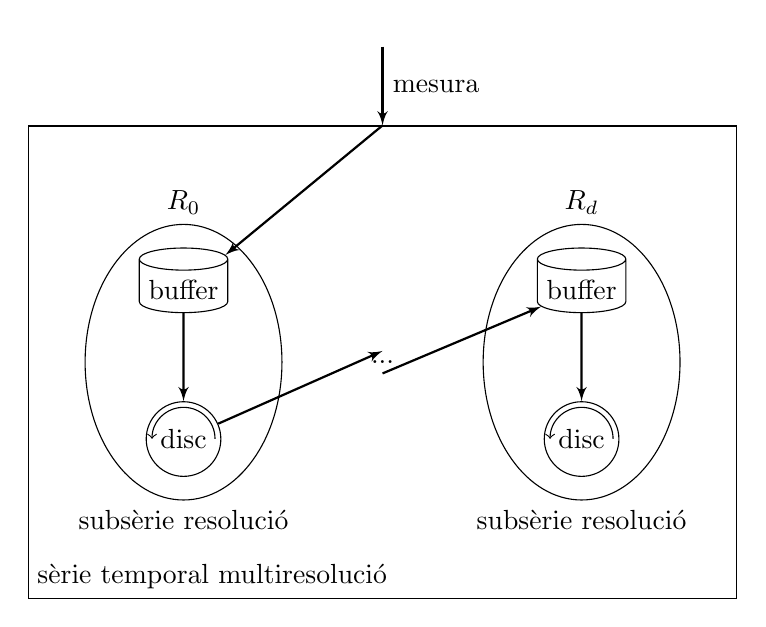
\begin{tikzpicture}
 \tikzset{
        myarrow/.style={->, >=latex',  thick},
      }
      

  \node[rectangle,draw,minimum height=6cm,minimum width=9cm] (m) {};
  \draw[shift=( m.south west)]   
  node[above right] {sèrie temporal multiresolució};


  %discmig
  \node (m.center) (discr1) {...};

  %discr
  
  \node[ellipse,draw,minimum height=3.5cm,minimum width=2.5cm,alias=discr0] [left=of discr1] {};
  \node[above=0cm of discr0.north] {$R_0$};
  \node[below=0cm of discr0] {subsèrie resolució};

  \node[cylinder, draw, shape border rotate=90, aspect=0.25,alias=buffer0] [below=3mm of discr0.north] {buffer};
  \node[circle, draw,alias=disc0]  [above=3mm of discr0.south] {disc} ;
  \draw [->] (disc0.center)++(.4:.4cm) arc(0:180:.4cm);
  \draw[myarrow] (buffer0.bottom) -- (disc0.north);


  %discrd

  \node[ellipse,draw,minimum height=3.5cm,minimum width=2.5cm,alias=discrd] [right=of discr1] {};
  \node[above=0cm of discrd] {$R_d$};
  \node[below=0cm of discrd] {subsèrie resolució};

  \node[cylinder, draw, shape border rotate=90, aspect=0.25,alias=bufferd] [below=3mm of discrd.north] {buffer};
  \node[circle, draw,alias=discd]  [above=3mm of discrd.south] {disc} ;
  \draw [->] (discd.center)++(.4:.4cm) arc(0:180:.4cm);
  \draw[myarrow] (bufferd.bottom) -- (discd.north);



  %mesura 
  \node[above=1cm of m.north] (m0) {};

  \draw[myarrow] (m0) -- (m.north) 
  node[right,midway] {mesura};

  \draw[myarrow] (m.north) -- (buffer0);
  \draw[myarrow] (discr1.south) -- (bufferd);
  \draw[myarrow] (disc0) -- (discr1.north);

\end{tikzpicture}
  \caption{Arquitectura encadenada d'una base de dades multiresolució}
  \label{fig:sgstm:encadenats}
\end{figure}


Respecte a l'estructura general, l'estructura encadenada restringeix
els passos de consolidació dels buffers i els cardinals màxims dels
discs. Els buffers que depenen d'una altra resolució han de tenir un
pas de consolidació múltiple de l'altra resolució i han de tenir un
període de buffer que estigui inclòs en el lapse de l'altra resolució.
A més les resolucions encadenades també han de ser coherents en la
funció d'agregació d'atributs, la qual pot ser que hagi de ser la
mateixa funció. Les resolucions encadenades requereixen un estudi més
profund que l'estructura general i poden encadenar pèrdues successives
significatives, com per exemple és el cas de calcular la mitjana
successivament que, per no ser associativa, no és el mateix que
calcular-la en dos buffers independents.


L'estructura de resolucions encadenades pot ser útil per a aplicacions
que necessitin distribuir l'emmagatzematge de les sèries temporals
multiresolució.  En l'estructura genèrica del model, cada mesura que
s'insereix a una base de dades ha d'inserir-se a totes les subsèries
resolució, és a dir que en cas d'un emmagatzematge distribuït tota la
sèrie temporal original s'ha de distribuir a cada subsèrie.  En canvi
en l'estructura de resolucions encadenades, la sèrie temporal original
primer es resumeix en una subsèrie resolució i és només aquest resum
el que es distribueix a la següent subsèrie resolució.  D'aquesta
manera l'emmagatzematge de les resolucions queda distribuït en
diferents nodes i a l'hora de respondre a una consulta només cal
recollir les resolucions ja resumides que es necessitin.
\textcite{deligiannakis07} proposen una estratègia similar de
disseminació de la informació per a xarxes de sensors.



%\subsubsection{Estructura d'exemple}


A continuació mostrem, mitjançant un exemple, la variació que comporten
les resolucions encadenades en el model de \gls{SGSTM}.


\begin{example} [Sèrie temporal multiresolució amb resolucions encadenades]
  \label{ex:multiresolucio:encadenada}

  Per a definir una sèrie temporal multiresolució amb resolucions
  encadenades és útil reprendre l'\autoref{ex:model:bdm-vistes} en què
  s'exemplifica una sèrie temporal multiresolució organitzada en
  vistes.

  En aquest cas la relació de sèries temporals i noms
  $M_2^{\text{series}}$ segueix sent la mateixa $M_2^{\text{series}}=
  ((S':\text{nom},S:\text{sèrie temporal}),\{
  (S_{B1},\{(26,0),(29,0)\}), (S_{D1},\{(10,0), (15,0), (20,0),
  (25,0)\}), (S_{D2},\{(10,0), (20,0)\} )\})$ llevat que no hi ha
  $S_{B2}$, i la sèrie temporal multiresolució amb noms com a domini
  dels atributs de sèries temporals $M_2^{\text{noms}}$ també és la
  mateixa $M_2^{\text{noms}}= ((S'_B:\text{nom},S'_D:\text{nom},
  \tau:\glssymbol{not:Rb}, \delta:\glssymbol{not:Rb},
  k:\glssymbol{not:N}, f:\text{funció} ),\{ (S_{B1},S_{D1},25 ,5 ,4
  ,\text{mitjana} ), ( \mathbf{S_{D1}},S_{D2},20 , 10 ,3 ,
  \text{mitjana} ) \})$ excepte que el buffer de la segona resolució
  és el disc de la primera $S_{D1}$, el qual el destaquem en negreta.
  Mostrem $M_2^{\text{series}}$ i $M_2^{\text{noms}}$ en forma de
  taula a la \autoref{fig:multiresolucio:exencadenat}.

  \begin{figure}[tp]
    \centering
    \begin{tabular}{|c|c|c|c|c|c|}
      \multicolumn{2}{c}{$M_2^{\text{noms}}$} \\ \hline
      $S'_B$  & $S'_D$ & $\tau$ & $\delta$ & $k$ & $f$ \\ \hline
      $S_{B1}$ & $S_{D1}$ & 25 & 5  & 4 & mitjana  \\
      $\mathbf{S_{D1}}$ & $S_{D2}$ & 20 & 10 & 3 & mitjana  \\ \hline
    \end{tabular}\qquad
    \begin{tabular}{|c|c|c|}
      \multicolumn{3}{c}{$M_2^{\text{series}}$} \\ \hline
      \multirow{2}{*}{$S'$}  &  \multicolumn{2}{c|}{$S$} \\ \cline{2-3}
      & $t$      & $v$  \\ \hline
      \multirow{2}{*}{$S_{B1}$} 
      & 26 & 0 \\ 
      & 29 & 0 \\ \hline
      \multirow{4}{*}{$S_{D1}$} 
      & 10 & 0 \\ 
      & 15 & 0 \\ 
      & 20 & 0 \\ 
      & 25 & 0 \\ \hline
      \multirow{2}{*}{$S_{D2}$} 
      & 10 & 0 \\ 
      & 20 & 0 \\ \hline
    \end{tabular}
    \caption{Taula d'una sèrie temporal multiresolució amb resolucions encadenades}
    \label{fig:multiresolucio:exencadenat}
  \end{figure}




  \begin{figure}[tp]
    \centering
    %\usetikzlibrary{shapes,arrows,positioning}
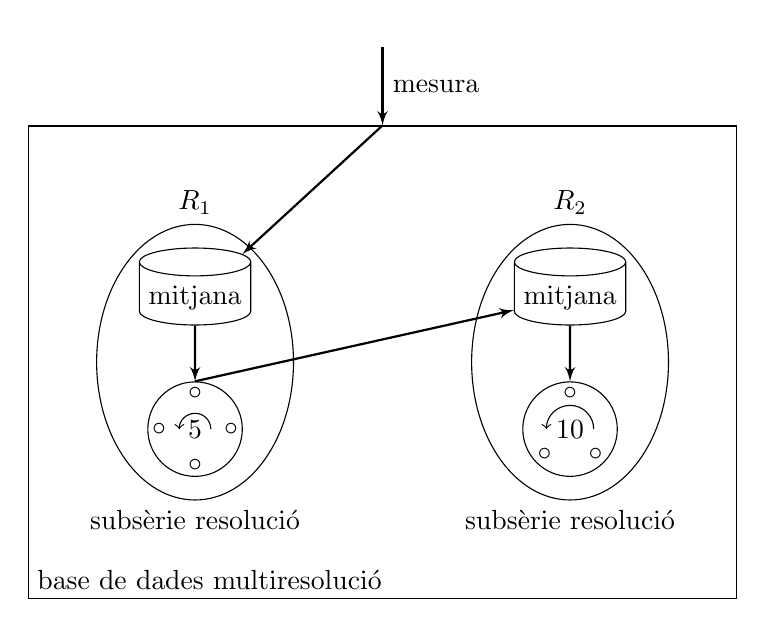
\begin{tikzpicture}
 \tikzset{
        myarrow/.style={->, >=latex',  thick},
      }
      

  \node[rectangle,draw,minimum height=6cm,minimum width=9cm] (m) {};
  \draw[shift=( m.south west)]   
  node[above right] {base de dades multiresolució};


  %discmig
  \node (m.center) (discr1) {};

  %discr
  
  \node[ellipse,draw,minimum height=3.5cm,minimum width=2.5cm,alias=discr0] [left=of discr1] {};
  \node[above=0cm of discr0.north] {$R_1$};
  \node[below=0cm of discr0] {subsèrie resolució};

  \node[cylinder, draw, shape border rotate=90, aspect=0.25,alias=buffer0] [below=3mm of discr0.north] {mitjana};
  \node[circle, draw,alias=disc0,minimum width=1.2cm]  [above=3mm of discr0.south] {5} ;
  \draw [->] (disc0.center)++(.2:.2cm) arc(0:180:.2cm);
  \draw[myarrow] (buffer0.bottom) -- (disc0.north);

  \node[circle,minimum width=9mm] (d0boles) [below=0mm of disc0.center,anchor=center] {};
  \node[below=0mm of d0boles.north,anchor=center] {$\circ$};
  \node[below=0mm of d0boles.east,anchor=center] {$\circ$};
  \node[below=0mm of d0boles.south,anchor=center] {$\circ$};
  \node[below=0mm of d0boles.west,anchor=center] {$\circ$};


  %discrd

  \node[ellipse,draw,minimum height=3.5cm,minimum width=2.5cm,alias=discrd] [right=of discr1] {};
  \node[above=0cm of discrd] {$R_2$};
  \node[below=0cm of discrd] {subsèrie resolució};

  \node[cylinder, draw, shape border rotate=90, aspect=0.25,alias=bufferd] [below=3mm of discrd.north] {mitjana};
  \node[circle, draw,alias=discd,minimum width=1.2cm]  [above=3mm of discrd.south] {10} ;
  \draw [->] (discd.center)++(.3:.3cm) arc(0:180:.3cm);
  \draw[myarrow] (bufferd.bottom) -- (discd.north);

  \node[circle,minimum width=9mm] (d1boles) [below=0mm of discd.center,anchor=center] {};
  \node[below=0mm of d1boles.north,anchor=center] {$\circ$};
  \node[below=0mm of d1boles.south east,anchor=center] {$\circ$};
  \node[below=0mm of d1boles.south west,anchor=center] {$\circ$};


  %mesura 
  \node[above=1cm of m.north] (m0) {};

  \draw[myarrow] (m0) -- (m.north) 
  node[right,midway] {mesura};

  \draw[myarrow] (m.north) -- (buffer0);
  
  %encadenada
  \draw[myarrow] (disc0.north) -- (bufferd);


\end{tikzpicture}
    \caption{Arquitectura de la base de dades multiresolució
      particular per l'exemple~\ref{ex:multiresolucio:encadenada}}
    \label{fig:multiresolucio:ex-arqu-encadenada}
  \end{figure}



  Se segueix aplicant la mateixa operació de $\text{vista } M_2$ que a
  l'\autoref{ex:model:bdm-vistes} per a obtenir la sèrie temporal
  multiresolució. A la \autoref{fig:multiresolucio:ex-arqu-encadenada}
  particularitzem l'arquitectura de la \autoref{fig:sgstm:encadenats}
  per a la base de dades d'aquest exemple. Cal, però, tenir dues
  consideracions en les operacions estructurals dels \gls{SGSTM} per a
  les resolucions encadenades: 

  \begin{itemize}
  \item L'operació d'inserció de mesures, $\glssymbol{addM}(M,m)$, no
    pot inserir la mesura a tots els buffers de les subsèries
    resolució sinó només a aquells que no estiguin encadenats. En el
    cas de l'exemple només al buffer $B_1$.  Aquests buffers, als
    quals podem anomenar buffers d'entrada, es poden expressar amb
    l'operació $ \glssymbol{not:sgst:project}_{\{S'_B\}}(
    M_2^{\text{noms}} ) -
    \glssymbol{not:sgst:rename}_{S'_D/S'_B}\left(
      \glssymbol{not:sgst:project}_{\{S'_D\}}( M_2^{\text{noms}}
      )\right)$.


  \item Només es poden eliminar les mesures dels buffers que no siguin
    encadenats, és a dir dels buffers d'entrada. Les resolucions
    encadenades només poden llegir les dades dels altres discs però
    no hi tenen control.

  \end{itemize}







\end{example}









\subsection{Funcions d'agregació amb orientació a flux}


Les funcions d'agregació d'atributs definides a
\textref{sec:model:agregador} operen sobre un interval de la sèrie
temporal i retornen una mesura que en resumeix un atribut. Aquesta
definició genèrica implica que els buffers han d'emmagatzemar
temporalment un conjunt de mesures de la sèrie temporal original i un
cop resumides les poden eliminar.

Això no obstant, es poden utilitzar els algoritmes d'orientació a
flux, com els que proposen \textcite{cormode08:pods}, per tal d'afitar
els cardinals dels buffers. Tot i així no totes les funcions
d'agregació d'atributs es poden implementar amb orientació a flux.




Definim una funció d'agregació amb orientació a flux, $f^\text{flux}$,
com aquella que implementa el comportament equivalent a una funció
d'agregació d'atributs $f$. A diferència de les $f$, treballen sobre
dues mesures $m'=f^\text{flux}(m_f,m,i)$ per a retornar la mesura
resultant $m'$, on $m$ és la nova mesura que s'ha d'incorporar al
flux, $m_f$ és el flux anterior ja processat i $i=[t_a,t_b]$ és
l'interval de consolidació de $f$.  Per exemple, redefinim les
funcions d'agregació \gls{dd} màxim i mitjana per tal que tinguin
orientació a flux:

\begin{itemize}
\item $\glssymbol{not:sgstm:maxdd}^\text{flux}: m_f \times m \times i \mapsto
  m'$ on $V(m')=\max(V(m_f),V(m))$ i $T(m')=\frac{t_b+t_a}{2}$. 


\item $\glssymbol{not:sgstm:mitjanadd}^\text{flux}: m_f \times m
  \times i \mapsto m'$ on $V(m') = V(m_f) + \frac{V(m)}{t_b-t_a}$ i
  $T(m')=\frac{t_b+t_a}{2}$.

\end{itemize}


Així, sigui $S=\{m_0,\dotsc,m_k\}$ una sèrie temporal i $i=[t_a,t_b]$
un interval de dos instants de temps, calcular en flux $m'_0 =
\glssymbol{not:sgstm:mitjanadd}^\text{flux}((0,0),m_0,i), m'_1 =
\glssymbol{not:sgstm:mitjanadd}^\text{flux}(m'_0,m_1,i), \dotsc, m'_k
= \glssymbol{not:sgstm:mitjanadd}^\text{flux}(m'_{k-1},m_k,i)$ és
equivalent a $m_k'=\glssymbol{not:sgstm:mitjanadd}(S,i)$, on $(0,0)$
és una mesura inicial per al flux.




Per a utilitzar en els \gls{SGSTM} les funcions d'agregació d'atributs
amb orientació a flux s'han de canviar els operadors d'afegir i de
consolidar dels buffers:



\begin{itemize}
\item Sigui la \autoref{def:sgstm:addB}, se'n modifica el comportament
  perquè $B=(m_B,\tau,\delta,f)$ sigui un buffer que emmagatzema una
  mesura $m_B$ en comptes d'una sèrie temporal i l'operació d'afegir
  sigui $\glssymbol{addB}(B,m)= (m'_B,\tau,\delta,f)$ on $m'_B =
  f^\text{flux}(m_B,m,[\tau,\tau+\delta])$ i $f^\text{flux}$ és una
  funció d'agregació d'atributs orientada a flux.


\item Sigui la \autoref{def:model:consolidacio-buffer}, se'n modifica
  el comportament perquè essent el buffer modificat
  $B=(m_B,\tau,\delta,f)$ l'operació de consolidar sigui
  $\glssymbol{consolidaB}(B) = (B',m_B)$ on
  $B'=(m'_B,\tau+\delta,\delta,f)$ i $m'_B$ ha de ser l'element
  d'identitat de $f^\text{flux}$. Per exemple $m'_B=(0,0)$ per a l'atribut
  de mitjana i $m'_B=(0,\min(\glssymbol{not:valor-domini}))$ per a
  l'atribut de màxim on $\glssymbol{not:valor-domini}$ és el domini
  dels valors. 

\end{itemize}

Així doncs, en l'orientació a flux de les funcions d'agregació
d'atributs, la mesura resultant es computa durant l'operació d'afegir
noves mesures al buffer i quan s'ha de consolidar el buffer el
resultat ja està disponible, només cal determinar l'element que actua
com a identitat per a la funció d'agregació amb flux.  En aquest cas,
no té sentit parlar de l'eliminació de mesures antigues en el buffer.










\subsection{Rellotge de consolidació}


En el model de \gls{SGSTM} no hi ha definit el concepte de rellotge,
és a dir no s'explicita quan s'ha de computar l'operació de
consolidar, si bé s'ha definit quan les sèries temporals
multiresolució esdevenen consolidables.  Les mesures tenen l'atribut
de temps i, si s'insereixen ordenades, ja marquen el pas del temps.
Tot i així, segons com sigui el rellotge i quan es computi l'operació
de consolidació hi pot haver els escenaris següents:

\begin{itemize}
\item Extern. Ho anomenem rellotge extern o \emph{push} perquè les
  mesures són les que controlen el procés de consolidació, de fet el
  controla un sistema de monitoratge extern.  El \gls{SGSTM} no té
  rellotge sinó que s'utilitza l'atribut de temps de les mesures per
  conèixer l'instant actual.  És el cas que hem definit en el model,
  en què una sèrie temporal multiresolució esdevé consolidable segons
  els instants de temps de les mesures adquirides i llavors ja pot ser
  consolidada. Per saber quan esdevé consolidable es pot consultar
  periòdicament o en base a esdeveniments, per exemple cada cop que
  s'insereixi una nova mesura.  Ja que el temps observat pel
  \gls{SGSTM} només canvia quan té mesures noves, això pot causar un
  cert decalatge de la consolidació de l'esquema amb un rellotge real,
  sobretot quan hi hagi inframostreig. 
  % es poden omplir els buffers?

\item Intern. Ho anomenem rellotge intern o \emph{pull} perquè el
  \gls{SGSTM} té un rellotge que controla el procés de consolidació.
  En aquests cas, la consolidació actua al marge del temps que
  indiquin les mesures i es computa quan ho marca el rellotge.  Això
  causa que la consolidació de l'esquema estigui totalment
  sincronitzada amb el rellotge real. En aquest cas s'hi poden
  incloure \gls{SGSTM} que controlin el procés d'adquisició, és a dir
  que ordenin quan s'han d'adquirir noves mesures. També es pot pensar
  en \gls{SGSTM} i istemes de monitoratge que no tinguin una bona
  mesura del temps actual, per exemple sense sincronització de
  rellotge, i en què l'objectiu dels \gls{SGSTM} sigui informar de
  l'evolució de les variables situant-les relativament a partir de
  l'instant en què es fa la consulta.




\end{itemize}

En el cas de les resolucions encadenades, com que depenen de la
consolidació d'un altre disc aquest aquest pot servir per a marcar el
rellotge. 


% * en cas de comptadors digitals, aquests cada cop que incrementen el valor poden fer un push a la base de dades. En comptadors analògics no ho poden fer perquè van incrementant contínuament i no discretament.







% \subsubsection{RRDtool}

% \todo{rrdtool?}
% Dibuixar l'esquema bàsic de RRDtool i comentar-lo aquí?


% Hi ha RRDtool, que és un SGBD específic dissenyat per a dades monitorades. Les c
% auses del seu disseny són:


% * Tobias Oetiker dissenyava un monitor de paràmetres de xarxes de comunicacions i en aquest monitor una part era la d'emmagatzematge de les dades. Per raons pràctiques i d'utilitat dissenya aquesta part amb un esquema inovadós. Finalment acaba separant aquesta part i la converteix independentment en RRDtool.

% * RRDtool té aquest model pràctic i a la pràctica és molt útil per a ser usat com a SGBD dels sistemes de monitoratge, sobretot en l'àmbit dels comptadors de xarxa on és l'estàndard de facto. 

% Això no obstant, no hi ha cap raonament teòric sobre el model de RRDtool ja que s'ha dissenyat per raons pràctiques. Per tant, entendre el funcionament de RRDtool és complicat, hi ha un nivell molt elevat per començar a fer-lo funcionar i molts conceptes no s'entenen perquè no estan ben definits. 

% Per això ens proposem de compendre i formalitzar el model de RRDtool, que acabarem anomenar model de multiresolució, en la teoria dels sitemes d'informació. A més RRDtool és molt específic pel camp de comptadors de xarxa i volem oferir un model genèric per a altres àmbits.  








%%% Local Variables: 
%%% mode: latex
%%% TeX-master: "main"
%%% End: 






%  LocalWords:  multiresolució


\chapter{Esquemes de multiresolució}

\todo{}


Definim una funció de multiresolució com una consulta sobre una sèrie
temporal que ens retorna una nova sèrie temporal resultant
d'aplicar-li un esquema de multiresolució. 

Aquesta funció de multiresolució ens permetrà:

\begin{itemize}
\item Plantejar problemes on veiem la multiresolució com una consulta sobre una sèrie temporal
\item Oferir sistemes duals de \glspl{SGSTM} i \glspl{SGST} amb operacions
  de consulta multiresolució.
\item Estudiar implementacions per a la consulta de multiresolució, p.ex. para\l.lelisme. (vegeu secció implementació \todo{})
\item Estudiar la teoria de la informació per a l'esquema de multiresolució
\end{itemize}






\section{Funció de multiresolució}

En el model de \gls{SGSTM} hem definit un model de dades de \gls{SGBD}
per a gestionar sèries temporals multiresolució. Com a \gls{SGBD},
aquest model té una estructura i per tant emmagatzema informació d'una
sèrie temporal en una forma determinada: la de multiresolució.  La
definició com a \gls{SGBD} té com a objectius l'emmagatzematge
compacte de les dades i la selecció de la informació ja preparada per
a consultes posteriors. 

Així, aquest model té capacitats de computació
sincronitzada o en línia (\emph{online}) amb el temps i té
característiques dels sistemes que tracten fluxos de dades (\emph{data
  stream}); és a dir dades que s'estan adquirint contínuament i cal
anar computant al mateix temps que es van adquirint. Això no treu,
però, que de manera més simplificada també es pugui treballar amb un
\gls{SGSTM} en temps diferit (\emph{offline}), és a dir que
s'emmagatzemin les dades adquirides i en el moment que es vulgui
aplicar-hi la consolidació.




Això no obstant, podem simplificar el problema de càlcul de
multiresolució en temps diferit com una consulta en un \gls{SGST} de
transformació d'una sèrie temporal a una nova sèrie temporal.

És a dir, sigui $S$ una sèrie temporal, $M$ una sèrie temporal
multiresolució i $e = \{ (\delta_0,f_0,\tau_0,k_0), \ldots,
(\delta_d,f_d,\tau_d,k_d)\}$ els paràmetres de l'esquema de
multiresolució de $M$. Afegim totes les mesures de la sèrie temporal a
la multiresolució, $\forall m \in S:
M=\glssymbol{addM}(M,m)$\todo{matemàticament és correcte recursivitat
  M=f(M)?}, i la consolidem, $M=\glssymbol{consolidaM}(M')$ fins que
$M$ no sigui consolidable. Consultem la sèrie temporal multiresolució
amb les dues consultes bàsiques, les quals retornen sèries temporals,
$S'=\glssymbol{not:sgstm:serietotal}(M')$ i $S_{\delta
  f}'\glssymbol{not:sgstm:seriedisc}(M',\delta,f)$ on $\delta$ i $f$
són dos paràmetres de l'esquema de multiresolució de $M$ que van
associats amb els altres dos corresponents $\tau$ i $k$.



Plantegem les funcions de transformació de la sèrie temporal original
a les consultades. És a dir, les funcions que anomenem
$\glssymbol{not:sgstm:dmap}$ i $\glssymbol{not:sgstm:multiresolucio}$
i que ens permeten calcular:

\[
\glssymbol{not:sgstm:dmap}: S \times \delta \times f \times \tau \times k \longrightarrow
S'_{\delta f}
\]


\[
 \glssymbol{not:sgstm:multiresolucio}: S \times e  \longrightarrow S'
\]



Definim la consulta de selecció de disc dels \gls{SGSTM} a partir del
mapatge dels \gls{SGST} de manera que, en computació per temps
diferit, són equivalents
\[
\glssymbol{not:sgstm:seriedisc}(M',\delta,f) \equiv
\glssymboldef{not:sgstm:dmap}(S,\delta,f,\tau,k)
\]


\begin{definition}[mapa de \glssymbol{not:sgstm:seriedisc}]
  Sigui $S$ una sèrie temporal, $M$ una sèrie temporal multiresolució
  amb esquema $e$ i $(\delta,f,\tau,k)\in e$ els paràmetres de
  multiresolució d'una subsèrie resolució. L'expressió de
  $\glssymbol{not:sgstm:seriedisc}(M,\delta,f)$ com a mapa d'una sèrie
  temporal és $\glssymboldef{not:sgstm:dmap}(S,\delta,f,\tau,k)=
  \glssymbol{not:sgst:map}(S_I,\glssymbol{not:sgst:fmap})$ on
  \[
  \glssymbol{not:sgst:fmap}: m_i\mapsto f(S, [T(m_i)-\delta,T(m_i)]),
  \]
  \[
  S_I = \{ (t,\infty) | t\in T_I  \},\;  t_M = T(\max(S)),
  \]
  \[
  T_I = \{ t_I = \tau+n\delta | n\in\glssymbol{not:Z}, t_M - k\delta <
  t_I \leq t_M \}.
  \]
\end{definition}



\begin{example}
  \label{ex:multiresolucio:dmap}
  Sigui la sèrie temporal $S=\{(1,0),(3,1),(6,0),(10,1)\}$ i els
  paràmetres de multiresolució
  $((\delta,5),(f,\glssymbol{not:sgstm:maxdd}),(\tau,0),(k,2))$.  El
  mapa de \glssymbol{not:sgstm:seriedisc} és una sèrie temporal $S'=
  \glssymboldef{not:sgstm:dmap}(S,5,0,\glssymbol{not:sgstm:maxdd},2)$
  on $S'=\{(5,1),(10,1)\}$. Expressem el càlcul pas a pas, a la
  \autoref{fig:multiresolucio:dmap} es visualitzen en taula les sèries
  temporals corresponents:
  \begin{enumerate}
  \item El primer pas és obtenir els instants de temps que
    s'emmagatzemarien al disc d'una sèrie temporal
    multiresolució. Així, els instants de consolidació possibles són
    $T_I'=\{\tau+n\delta|n\in\glssymbol{not:Z}\}=
    \{\ldots,-5,0,5,10,15,\ldots\}$. Però un cop consolidat el disc
    només hi haurà els $k=2$ més recents abans de $t_M=T(\max(S))=10$,
    és a dir $T_I=\{t_I'\in T_I'|t_M - k\delta < t_I \leq
    t_M\}=\{5,10\}$.

  \item El segon pas és obtenir a partir de $T_I$ la sèrie temporal
    $S_I$ que es correspon amb la sèrie temporal que s'inicialitzaria
    al disc encara amb valors desconeguts,
    $S_I=\{(5,\infty),(10,\infty)\}$.



  \item El tercer pas és calcular la funció d'agregació a $S$ per a
    cada intervals de consolidació del disc de la forma
    $[T(m_i)-\delta,T(m_i)]$ on $m_i\in S_i$, és a dir $f(S,[0,5])$ i
    $f(S,[5,10])$. A tal efecte utilitzem el mapa sobre $S_I$ per a
    calcular la sèrie temporal resultant $S'=\{ (5,f(S,[0,5])),
    (10,f(S,[5,10])) \}$.

    Podríem calcular un pas entremig que es correspon amb les sèries
    temporals que hi hauria en el buffer abans de cada instant de
    consolidació. Així, per a cada $T(m_i)$ hi hauria la sèrie
    temporal $S[T(m_i)-\delta,T(m_i)]$, és a dir $S_B=\{
    (5,S[0,5],(10,S[5,10]) \}$.
  \end{enumerate}


  


\begin{figure}[tp]
  \centering
  \begin{tabular}[c]{|c|c|}
    \multicolumn{2}{c}{$S$} \\ \hline
    $t$  & $v$ \\ \hline
    1  & 0 \\
    3  & 1 \\
    6  & 0 \\
    10  & 1 \\ \hline
  \end{tabular} \qquad
  \begin{tabular}[c]{|c|c|}
    \multicolumn{2}{c}{$S_I$} \\ \hline
    $t$  & $v$ \\ \hline
    5  & $\infty$ \\
    10  & $\infty$ \\ \hline
  \end{tabular} \qquad
  \begin{tabular}[c]{|c|c|}
    \multicolumn{2}{c}{$S_B$} \\ \hline
    $t$  & $v$ \\ \hline
    5  & \begin{tabular}[c]{|c|c|}\hline $t$  & $v$ \\ \hline 1&0\\ 3&0 \\\hline  \end{tabular} \\\hline
    10  & \begin{tabular}[c]{|c|c|}\hline $t$  & $v$ \\ \hline 6&0\\ 10&1 \\\hline  \end{tabular} \\ \hline
  \end{tabular} \qquad
 \begin{tabular}[c]{|c|c|}
    \multicolumn{2}{c}{$S'$} \\ \hline
    $t$  & $v$ \\ \hline
    5  & 1 \\
    10  & 1\\ \hline
  \end{tabular}
  \caption{Taules de les sèries temporals per l'operació de mapa de  \glssymbol{not:sgstm:seriedisc}}
  \label{fig:multiresolucio:dmap}
\end{figure}
 
\end{example}





Definim la consulta de sèrie temporal total dels \gls{SGSTM} a partir
del plegament dels \gls{SGST} de manera que, en computació per temps
diferit, són equivalents
\[
\glssymbol{not:sgstm:serietotal}(M') \equiv \glssymbol{not:sgstm:multiresolucio}(S,e)
\]

\begin{definition}[plec de \glssymbol{not:sgstm:serietotal}]
  Sigui $S$ una sèrie temporal i $M$ una sèrie temporal multiresolució
  amb esquema $e = \{ (\delta_0,f_0,\tau_0,k_0), \ldots,
  (\delta_d,f_d,\tau_d,k_d)\}$, el qual es pot observar com una sèrie
  temporal multivaluada.  L'expressió de
  $\glssymbol{not:sgstm:serietotal}(M)$ com a plec d'una sèrie
  temporal és $\glssymboldef{not:sgstm:multiresolucio}(S,e)=
  \glssymbol{not:sgst:ofold}(e,\{\},\glssymbol{not:sgst:ffold},\min)$
  on $\glssymbol{not:sgst:ffold}: S_i \times (\delta_c,f_c,\tau_c,k_c)
  \mapsto S_i ||
  \glssymbol{not:sgstm:dmap}(S,\delta_c,f_c,\tau_c,k_c)$.

  Així, el plec de \glssymbol{not:sgstm:serietotal} és la concatenació de
  tots els \glssymbol{not:sgstm:dmap} possibles per l'esquema $e$
  ordenats per $\delta$, assumint que $e$ no conté $\delta$ repetits.
\end{definition}



En resum: en temps diferit, s'insereixen les mateixes mesures a un
\gls{SGST} i a un \gls{SGSTM}. Per una banda es consolida el
\gls{SGSTM} i s'obté la sèrie total i per altra banda es consulta la
multiresolució en el \gls{SGST}. Aleshores s'obté la mateixa sèrie
temporal.


\begin{example}
  Sigui la sèrie temporal $S=\{(1,0),(3,1),(6,0),(10,1)\}$ i l'esquema
  de multiresolució
  $e=\{\{(\delta,5),(f,\glssymbol{not:sgstm:maxdd}),(\tau,0),(k,2)\},
  \{(\delta,2),(f,\glssymbol{not:sgstm:maxdd}),(\tau,0),(k,3)\}\}$.
  El plec de $\glssymbol{not:sgstm:serietotal}$ és una sèrie temporal
  $S'= \glssymboldef{not:sgstm:multiresolucio}(S,e)$ on
  $S'=\{(5,1),(6,0),(8,0),(10,1)\}$. Expressem el càlcul pas a pas, a la
  \autoref{fig:multiresolucio:multiresolucio} es visualitzen en taula les sèries
  temporals corresponents:

  \begin{enumerate}
  \item En primer lloc es calcula la sèrie temporal pels paràmetres de
    multiresolució $\delta_1$:
    $S_{D1}=\glssymbol{not:sgstm:dmap}(5,\glssymbol{not:sgstm:maxdd}),0,2)=\{(5,1),(10,1)\}$,
    com ja s'ha vist a l'\autoref{ex:multiresolucio:dmap}.

  \item En segon lloc, es calcula la sèrie temporal pels paràmetres de
    multiresolució $\delta_2$:
    $S_{D2}=\glssymbol{not:sgstm:dmap}(2,\glssymbol{not:sgstm:maxdd}),0,3)=\{(6,0),(8,0),(10,1)\}$,
    de manera similar a $S_{D1}$.

  \item En tercer lloc es concatenen les sèries temporals per ordre de
    $\delta$: $\delta_2<\delta_1$. Així, $S'= S_{D2} || S_{D1}$.

  \end{enumerate}
  


\begin{figure}[tp]
  \centering
  \begin{tabular}[c]{|c|c|}
    \multicolumn{2}{c}{$S$} \\ \hline
    $t$  & $v$ \\ \hline
    1  & 0 \\
    3  & 1 \\
    6  & 0 \\
    10  & 1 \\ \hline
  \end{tabular} \qquad
  \begin{tabular}[c]{|c|c|}
    \multicolumn{2}{c}{$S_{D1}$} \\ \hline
    $t$  & $v$ \\ \hline
    5  & 1 \\
    10  & 1 \\ \hline
  \end{tabular} \qquad
  \begin{tabular}[c]{|c|c|}
    \multicolumn{2}{c}{$S_{D2}$} \\ \hline
    $t$  & $v$ \\ \hline
    6  & 0 \\
    8  & 0 \\
    10  & 1 \\ \hline
  \end{tabular} \qquad
  \begin{tabular}[c]{|c|c|}
    \multicolumn{2}{c}{$S'$} \\ \hline
    $t$  & $v$ \\ \hline
    5  & 1 \\
    6  & 0 \\
    8  & 0 \\
    10  & 1 \\ \hline
  \end{tabular}
  \caption{Taules de les sèries temporals per l'operació de plec de  \glssymbol{not:sgstm:serietotal}}
  \label{fig:multiresolucio:multiresolucio}
\end{figure}
 


\end{example}








\subsection{Demostració}

Cal demostrar l'equivalència formalment\todo{}





\section{Sistemes duals amb SGST i SGSTM}
\todo{}



Oferir sistemes duals de \gls{SGSTM} i \gls{SGST} amb operacions
  de consulta multiresolució.




* Sistemes on el SGSTM funcionen com a cache per a consultes multiresolució, cache de consultes que mai s'han fet però que s'ha previst que es puguin fer -> computació en flux

* Sistemes on la informació en un warehouse SGST (que es consulta rarament) serveix per si es vol fer un canvi d'esquema  en un SGSTM poder recalcular les dades que hi hauria hagut en el SGSTM. Altrament el SGSTM ha de començar de nou. Pensem en un canvi d'esquema com per exemple ampliar un disc o canviar la $f$, un canvi com reduir un disc sí que es pot recalcular

* Posar símil amb la compressió multimèdia: es tenen fitxers lossless que s'emmagatzemen i es fan servir rarament, es fan circular fitxers lossy que ocupen menys i són més àgils per treballar; en el cas que calgui modificar un lossy  es regenera un de nou a partir del lossless. Sobretot es fa per evitar les pèrdues encadenades entre compressions lossy.


\todo{notar que els SGSTM es basen en els SGST}



La multiresolució(S) és una operació computada en temps diferit.

La SèrieTotal(S) és una operació computada en línia, és a dir seguint el flux de $S$. El temps de comput no és tant crític perquè es reparteix al llarg del temps, és a dir tal com es van adquirint les dades; més enllà del temps de càlcul de cada funció d'agregació: aquest limita quantes sèries temporals multiresolució diferents i quantes resolucions de cada es poden emmagatzemar un mateix aparell.





% \subsection{Two database structures}

% \acro{MTSMS} imply a data information selection and so the information
% not considered important is discarded.  Therefore, this systems are
% not adequate when all the monitored data must be kept as
% acquired. This can happen for example when it is not known a priori
% which aggregate functions will work better with the future data
% monitored or when detailed questions must be retrieved such as at what
% hour exactly an event triggered. 

\begin{figure}
  \centering
  %\usetikzlibrary{shapes,arrows,positioning}
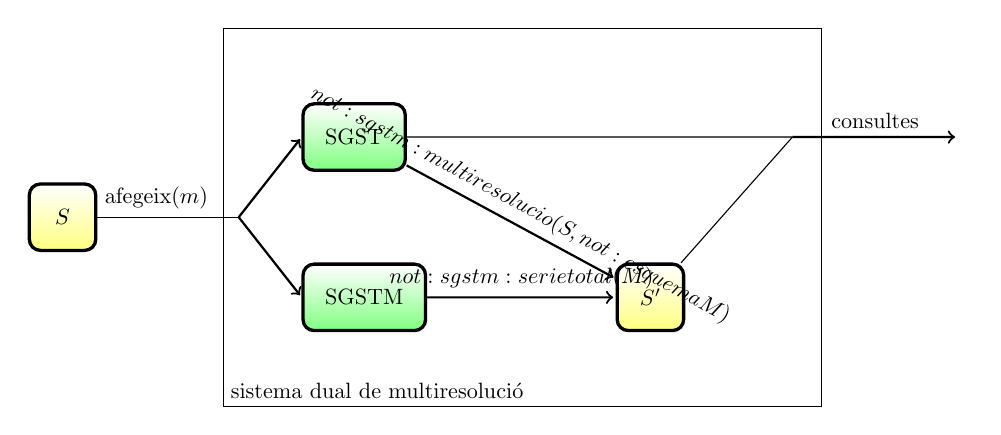
\begin{tikzpicture}[scale=0.8, every node/.style={transform shape}]

      \tikzset{
        mynode/.style={rectangle,rounded corners,draw=black, 
          very thick, inner sep=1em, minimum size=3em, text centered,
          groc},
        myarrow/.style={->, shorten >=1pt, thick},
        mylabel/.style={text width=7em, text centered},
        groc/.style={top color=white, bottom color=yellow!50},
        verd/.style={top color=white, bottom color=green!50},
        roig/.style={top color=white, bottom color=red!50},
      }  






 \node[mynode] (m) {$S$};

 \node[right=2cm of m] (mdins) {};

 \node[mynode, verd, above right=0.6cm and 1cm of mdins] (tsms) {\glstext{SGST}};

 \node[mynode, verd, below right=0.6cm and 1cm of mdins] (mtsms) {\glstext{SGSTM}};

 \node[rectangle,draw,minimum height=6cm,minimum width=9.5cm,right=-0.25cm of mdins] (dual) {};

\draw[shift=( dual.south west)]   
  node[above right] {sistema dual de multiresolució};






 \node[mynode,right=3cm of mtsms] (ts) {$S'$};



 \draw (m.east) -- (mdins.east) node[above right,at start]
 {afegeix$(m)$};

 \draw[myarrow] (mdins.east) -- (tsms.west);
 \draw[myarrow] (mdins.east) -- (mtsms.west);


 \draw[myarrow] (tsms) -- (ts) node[above,midway,sloped]
 {$\glssymbol{not:sgstm:multiresolucio}(S,\glssymbol{not:esquemaM})$}; 
 
 \draw[myarrow] (mtsms) -- (ts) node[above,midway,sloped]
 {$\glssymbol{not:sgstm:serietotal}(M)$};




 \node[right=6cm of tsms] (consdins) {};

 \draw (tsms) -- (consdins.center);
 \draw (ts) -- (consdins.center);

 \node[right=2.5cm of consdins] (consultes) {};
 \draw[myarrow] (consdins.center) -- (consultes) node[above,midway,sloped]
 {consultes};



\end{tikzpicture}



%%% Local Variables:
%%% TeX-master: "../main"
%%% End:

  \caption{Sistema dual \gls{SGST}+\gls{SGSTM}}
  \label{fig:multiresolucio:dual}
\end{figure}

% This may be overcome with dual \acro{DBMS} that share measure input,
% as shown in Figure~\ref{fig:model:mtsms-tsms}. One is a \acro{TSMS}
% for long-term deposit and only consulted in occasional cases, it can
% be \acro{TSMS} with other compression techniques or large size
% \acro{DBMS}. The other is a \acro{MTSMS} that lossy compresses time
% series.

% Then generic queries can be made from \acro{TSMS} information or from
% \acro{MTSMS} selected information, as instance by TotalSeries. In
% Figure~\ref{fig:model:mtsms-tsms} the logical equivalence of applying
% $S'=\totalseries(M)$ to \acro{MTSMS} and $S'=
% \multiresolution(S,\text{sch})$ to \acro{TSMS} is plotted, however the
% implementation consideration are different. If we regard the resulting
% time series $S'$ as a view of database information, then the
% $\multiresolution$ is a view that must be computed fully at every new
% measure addition and $\totalseries$ is a view that can be computed
% incrementally at every new addition as explained next.


% Time series data volume uses to be very big and increases along
% time. However, this increase is due to a continuous acquisition of
% data. When data comes as an ordered sequence of instances it is called
% data stream, then specific \acro{DBMS} are designed to manage data
% stream data \cite{stonebraker05:sigmod}.  \acro{MTSMS} can take
% advantage of data stream orientation in order to simplify the
% consolidation process.  Assuming a time order acquisition of time
% series, the update of a \acro{MTSMS} only consists in the addition of
% new measures and the incremental consolidation of subseries.  As a
% consequence \acro{MTSMS} can be seen as a time series view
% pre-computing system for a pair of aggregation statistics and time
% resolution operations.  Then this pre-computation can be used for
% another queries, limited to the aggregations previously computed, or
% for graphical visualisations like the ones done by RRDtool
% \cite{rrdtool}.

% We then have showed a structure for manipulating in time order as then there are no updates in data and it can be managed more simpler. 

%* Important! dir que si seguim l'addició amb ordre de les mesures, aleshores es pot fer l'stream en els MTSMS ja que no hi ha possibilitat d'operacions d'UPDATE.




\subsection{Conceptes relacionats}


\textcite{marz13:nosql13, marz14:bigdata} generalitzen un concepte
similar al de \gls{SGST} dual, ho emmarquen en l'àmbit dels \gls{SGBD}
per a \emph{Big Data}.  Proposen \gls{SGBD} dissenyats amb tres
nivells, que anomenen arquitectura \emph{Lambda}:
\begin{itemize}
\item Nivell \emph{batch}: Emmagatzema totes les dades originals i
  permet realitzar qualsevol consulta sobre aquestes dades. Preveu que
  algunes consultes operen sobre dades consultades prèviament, per
  tant en aquest nivell es gestionen també aquestes consultes
  precomputades, les quals a més es poden obtenir amb computació
  para\l.lela com per exemple amb Hadoop. Particularment, es considera
  que les dades originals són immutables, és a dir que les bases de
  dades només permeten afegir però no modificar.

\item Nivell \emph{server}: Emmagatzema les consultes precomputades i
  n'ofereix les dades per a altres consultes. Les consultes
  precomputades s'han de tornar a calcular periòdicament i en el
  nivell \emph{server} sempre hi ha la versió calculada més
  recent. Per tant, es preveu que les consultes precomputades no
  ofereixen la informació actualitzada al moment, sinó que hi ha un
  cert temps des que es modifiquen les dades originals fins que té
  impacte en les consultes.

\item Nivell \emph{speed}: Precomputa les mateixes consultes que el
  nivell \emph{batch} però incrementalment, és a dir cada cop que
  s'afegeix una dada nova les dades de la consulta \emph{speed}
  s'actualitzen adequadament.  Aquest nivell només s'usa per a dades
  recents per tal complementar el problema de les dades
  desactualitzades en els nivells \emph{batch} i \emph{server}.
\end{itemize}


Les consultes precomputades d'aquests sistemes semblen una bona
solució per a la computació de les vistes dels \gls{SGBDR}.  Una vista
és un àlies per a una expressió relacional, és a dir una consulta, que
s'utilitza en altres consultes. Per tant, una vista $v$ és una
operació $\text{op1}$ sobre unes $\text{dades}$,
$v:=\text{op1}(\text{dades})$, i s'utilitza una altra consulta
$\text{op2}(v)$ de manera que és equivalent a executar la consulta
$\text{op2}(\text{op1}(\text{dades}))$. Així doncs, el model de vistes
és similar a les consultes que es basen en altres consultes proposat
per \citeauthor{marz14:bigdata} o a les sèries temporals precomputades
que proposem.


En el model relacional \cite[cap.~10. Views]{date04:introduction8} es
considera, conceptualment, que les vistes no s'avaluen quan es
defineixen sinó cada cop que s'executa una consulta que hi opera.  En
les implementacions les vistes poden ser precomputades, aleshores
s'anomenen \emph{snapshots} o \emph{materialized views}, per tal
d'aconseguir un emmagatzematge temporal dels mateixos càlculs per a
diverses consultes. En el context de sistemes de suport a les
decisions, la precomputació també es preveu en el càlcul de taules
resum per a agregacions de les dades \cite[cap.~22. Decision
support]{date04:introduction8}.  Això no obstant, la precomputació de
vistes no sempre comporta una millor eficiència; el concepte de vista
del model permet la substitució algebraica i per tant permet
l'optimització global de la consulta i l'operació continguda a la
vista.


Les vistes precomputades tenen associada una acció per actualitzar de
nou el seu valor. En usar vistes precomputades cal preveure el termini
de validesa dels càlculs precomputats, com ocorre en el nivell
\emph{server} de l'arquitectura \emph{Lambda}. Així doncs, les vistes
precomputades es poden actualitzar de vàries maneres:
\begin{itemize}

\item Es computen periòdicament, com també es proposa en el nivell
  \emph{batch} de l'arquitectura \emph{Lambda}.

\item Es computen cada cop que es modifiquen les dades amb les quals operen, per
  exemple mitjançant operacions de \emph{trigger}. \todo{Els indexos
    als SGBD fan una cosa similar a això?}

\item Quan es modifiquen les dades, s'aplica la mateixa
  operació a la vista precomputada. És a dir, quan es modifiquen les
  dades originals amb una operació $\text{mod}(\text{dades})$ es
  trasllada aquesta operació a la vista $\text{mod}'(\text{dades})$ on
  cal determinar la relació entre $\text{mod}$ i $\text{mod}'$.  És el
  que es proposa en el nivell \emph{speed} de l'arquitectura
  \emph{Lambda} i el que admet el model de \gls{SGSTM} que proposem.
\end{itemize}





% \subsection{Stream orientation}

% \todo{}
% * Dues variacions possibles interessants pels MTSMS:

 
%   - Buffers com a streams, sempre de mida fitada 
%   - Discos enllaçats





%%% Local Variables:
%%% TeX-master: "main"
%%% End:






%  LocalWords:  multiresolució

\chapter{Reflexions sobre la informació en la multiresolució}
\label{sec:multiresolucio:teoriainformacio}


En aquest capítol reflexionem sobre el problema de la qualitat en la
multiresolució de sèries temporals, és a dir sobre el problema
d'identificar la informació que selecciona un esquema de
multiresolució i per tant, alhora, d'observar quina informació no
queda emmagatzemada i es perd.  Contextualitzem aquest problema en
l'aplicació de la teoria de la informació per a l'esquema de
multiresolució.

En aquest context, els \gls{SGSTM} són un sistemes que emmagatzemen
dades comprimides amb pèrdua d'una certa part de la informació
original. Aleshores, les consultes que es resolen a partir d'un
\gls{SGSTM} són consultes aproximades a la informació total original,
llevat que mitjançant una anàlisi determinem que poden oferir
consultes exactes. A continuació reflexionem sobre com analitzar
l'error de les consultes de multiresolució respecte a la informació
original:
\begin{itemize}
\item Primer, descrivim de forma molt genèrica la teoria de la
  informació, la qual està relacionada amb la quantificació de la
  informació.
\item Segon, definim el problema de calcular l'error en la multiresolució.
\item Tercer, mostrem exemples d'anàlisi de la informació per alguns
  esquemes de multiresolució.
\end{itemize}





\section{Quantificació de la informació}

En altres àmbits, la teoria de la informació (\emph{information
  theory}) és el referent per a formalitzar la quantificació de la
informació. És també el cas de la compressió de dades, un àmbit proper
als \gls{SGSTM} en aquest context d'informació.  Per al cas particular
de compressió amb pèrdua s'aplica un subconjunt de la teoria anomenat
teoria de la taxa de
bit-distorsió %optimot: rate-distortion relationship
(\emph{rate–distortion theory}); la qual modela la percepció de la
distorsió i valora l'estètica dels resultats.


Per a quantificar la informació d'unes dades s'utilitza l'entropia, la
qual mesura la incertesa de predir els valors de les dades. Així, com
més entropia més aleatòries són les dades i com menys, més
redundants. Si l'entropia és zero aleshores les dades són totalment
predictible; és a dir donat un valor es coneix exactament quin és el
següent.




La compressió redueix la mida original de les dades. En el cas de la
compressió sense pèrdua es conserva la informació però s'augmenta
l'entropia, és a dir que s'elimina la redundància de les dades, i en
el cas de la compressió amb pèrdua es descarta informació que es
considera no essencial, per exemple en una imatge detalls que l'ull
humà no pot apreciar, tot i que també poden transformar les dades a un
altre domini on es es percebi millor la informació, per exemple
treballar en el domini freqüencial del so per a operacions
d'equalització. Aquesta aplicació de la compressió amb pèrdua per tal
de representar millor les dades també es coneix amb el nom de
codificació perceptiva (\emph{perceptual encoding}).



Els mètodes de compressió amb pèrdua se solen usar per a compressió de
multimèdia. L'objectiu és aconseguir menys volum de dades però que
conservin la mateixa percepció que les originals, o fins i tot amb una
pèrdua de qualitat perceptible mentre compleixi amb els requisits de
l'aplicació que se li vol donar. Així doncs, la compressió de
multimèdia sovint requereix valorar la percepció humana, per tal de
valorar la qualitat de percepció humana s'utilitzen testos subjectius
en què un humà ha d'intentar distingir entre multimèdia original i
multimèdia comprimit.
%  com per exemple el test
% ABX\todo{ref}.  %http://en.wikipedia.org/wiki/ABX_test
%http://web.archive.org/web/20070813001013/http://www.pcabx.com/


%  Lossy methods are most often used for compressing sound, images or videos. This is because these types of data are intended for human interpretation where the mind can easily "fill in the blanks" or see past very minor errors or inconsistencies – ideally lossy compression is transparent (imperceptible), which can be verified via an ABX test. http://en.wikipedia.org/wiki/ABX_test
% Flaws caused by lossy compression that are noticeable to the human eye or ear are known as compression artifacts.




% \todo{information algebra}
% \url{https://en.wikipedia.org/wiki/Information_algebra}

% algebra of information, describing basic modes of information processing. Such an algebra involves several formalisms of computer science, which seem to be different on the surface: relational databases, multiple systems of formal logic or numerical problems of linear algebra. It 



% El procediment
% que se segueix és: comprimir, emmagatzemar, descomprimir i
% visualitzar.
% compressed data must be decompressed to use -> en els sgstm no? bé si vull veure tota la sèrie temporal sí que he de concatenar el que hi tinc i per tant es pot veure com una descompressió (al marge que hi pot haver una compressió/descompressió en els agregadors usats, per exemple si és un so emmatgatzemar la freqüència i després s'haurà de descomprimir a amplitud al llarg del temps).
% The design of data compression schemes involves trade-offs among various factors, including the degree of compression, the amount of distortion introduced (e.g., when using lossy data compression), and the computational resources required to compress and uncompress the data.
% * No hi ha descompressió. Els algoritmes de compressió amb pèrdua normalment van associats amb les tècniques de compressió/descompressió; és a dir que les dades s'emmagatzemen amb estructures intermitges, que ocupen menys mida, i que cal descomprimir per recuperar-les. En els cas dels SGSTM les dades s'emmagatzemen com a subsèries temporals en els discs i per tant a l'hora de recuperar-les ja són sèries temporals, com a molt potser fa falta concatenar-les per a obtenir tota la sèrie temporal.



% The main drawback of lossy compression techniques is that they
% rely on specific patterns for providing a good approximation of the given time series.
% This is the main reason why lossy compression has been rarely applied to network
% monitoring contexts, where the patterns of time series can drastically change due to
% anomalous events or to transient networking issues.

%http://www.data-compression.com/theory.shtml


\section{Error en la informació de la multiresolució}

El model dels \gls{SGSTM} es basa en una compressió amb pèrdua, és a
dir descartar dades i emmagatzemar només aquella informació que es
consideri necessària o suficient. Així doncs, cal quantificar quin
error hi ha entre la informació emmagatzemada i la informació que
contenen les dades originals.


El problema genèric de la informació en la multiresolució és el següent.
\begin{definition}[Error en la informació de la multiresolució]
  \label{def:informacio:error}
  Sigui una sèrie temporal $S$ i una sèrie temporal multiresolució $M$
  resultant de l'emmagatzematge i consolidació de $S$. De la sèrie
  temporal multiresolució es pot consultar la sèrie temporal total
  $S'=\glssymbol{not:sgstm:serietotal}(M)$ o bé de forma equivalent,
  com s'ha descrit en \textref{cap:funciomultiresolucio},
  $S'=\glssymbol{not:sgstm:multiresolucio}(S,e)$ on $e$ és l'esquema
  de $M$.  S'executa una operació de consultam, $o$, sobre la sèrie
  temporal original, $r_1=o(S)$, i la mateixa operació sobre la sèrie
  temporal de la multiresolució, $r_2=o(S')$. Es pot avaluar l'error
  de multiresolució $\epsilon=d(r_1,r_2)$ on $d$ és una funció que
  permet avaluar la distància entre els dos resultats.
\end{definition}


Cal aclarir que es podria avaluar $d(S,S')$, però aquest no és el
problema que intenten resoldre els \gls{SGSTM}. Aquest seria un
problema d'aproximació al senyal original, el qual altres models poden
resoldre més bé com per exemple \textcite{last01,ogras06}. En canvi
els \gls{SGSTM} resolen un problema de compressió amb pèrdua per a
seleccionar una determinada informació. És en aquest context que
proposem l'error en la informació de la multiresolució en què avaluem
$d(r_1,r_2)$.



Per a avaluar la distància $d(r_1,r_2)$, si els resultats d'ambdues
consultes són sèries temporals, es pot utilitzar per exemple mínims
quadrats com fa \textcite{last01}.  Ara bé, en la informació de la
multiresolució cal pensar també amb consultes qualitatives. Per
exemple una consulta podria ser $o=$`Creix la sèrie temporal?'
Aleshores no hi hauria error $\epsilon=d(r_1,r_2)$ quan la resposta
fos la mateixa per als dos casos, $r_1$ i $r_2$, i hi hauria error
quan les respostes diferissin.


Tot i que hem proposat d'aplicar la mateixa operació $o$ a la sèrie
temporal original $r_1=o(S)$ i a la sèrie temporal de la
multiresolució $r_2=o(S')$, pot ser que l'operació hagi de ser
diferent per a obtenir el mateix resultat. És a dir $r_1=o(S)$ però
$r_2=o'(S')$ on $o'$ és l'operació equivalent a $o$ per aplicar
després de la multiresolució.  Per exemple, una operació $o$ podria
ser el càlcul de la multiresolució,
$r_1=\glssymbol{not:sgstm:multiresolucio}(S,e)$, aleshores l'operació
$o'$ equivalent és la identitat perquè el \gls{SGSTM} ja ha calculat
la multiresolució, $r_2=S'$. Aquest exemple, de fet, és el cas que hem
formulat a la \autoref{sec:multiresolucio:funcio}, on hem descrit que
és equivalent la sèrie temporal emmagatzemada en un \gls{SGSTM} a
aplicar la funció \glssymbol{not:sgstm:multiresolucio} a una sèrie
temporal; per tant l'error $\epsilon =d(r_1,r_2)$ seria nul.



Així doncs, l'error en la informació de la multiresolució permet
quantificar la pèrdua d'informació dels \gls{SGSTM}. Un cop
quantificat l'error per a un determinat esquema de multiresolució es
pot saber per a quines consultes serà apropiat aquell esquema i per a
quines no. Per a quantificar aquest error es poden preveure diversos
contextos:
\begin{itemize}
\item Hi ha consultes que es poden resoldre a la perfecció, és a dir
  sense error. Per exemple és el cas descrit on l'operació que es vol
  fer a una sèrie temporal és precisament la consulta de
  multiresolució.
  %altres exemples, per exemple en el cas de comptadors per a consultar totals

\item Es pot calcular l'error mesurant la diferència entre la mateixa
  consulta aplicada a les dades originals que a les dades
  emmagatzemades en el \gls{SGSTM}.

\item Es pot avaluar subjectivament l'error mitjançant la
  visualització de les dades. És a dir, de manera semblant a la
  compressió amb pèrdua de multimèdia, l'usuari valora subjectivament
  si visualitza la mateixa informació en les dades originals com en
  les dades comprimides amb multiresolució. Per exemple, un dels
  criteris que recomana RRDtool per a establir un esquema de
  multiresolució és tenir en compte l'amplada de la pantalla on es
  visualitzen els resultats: no cal treballar amb una sèrie temporal
  amb molta resolució si no és possible observar-la \parencite[Rates,
  normalizing and consolidating]{vandenbogaerdt} .
  % RRDtool expliquen un criteri que és definir les k dels discs inferior a l'amplada en píxels de la pantalla. Aquest és un criteri basat en una consulta per a fer visualització immediatament. Llavors no té sentit tenir més nombre de dades que les que es poden visualitzar.  Per exemple si capturem dades cada 5 minuts al llarg d'un any obtenim 43800 punts; si no disposem d'un monitor amb aquest nombre de píxels d'amplada no els podrem percebre.
  %Això potser també té relació amb el camp de gràfics 3D, on la multiresolució s'aplica per a no treballar amb objectes que només seran percebuts com un píxel?

\end{itemize}






\section{Exemples d'anàlisi de la informació}


La \autoref{def:informacio:error} defineix el problema d'informació en
la multiresolució de forma genèrica i abstracta. Així, en cada context
d'aplicació de la multiresolució cal interpretar-ne el significat i
particularitzar-ne un mètode d'anàlisi adequat.  A tal efecte, a
continuació proposem alguns exemples que mostren casos particulars
d'anàlisi de la selecció o pèrdua d'informació que hi ha en un
\gls{SGSTM}.


Per a simplificar els exemples, proposem esquemes de multiresolució amb
només una resolució i amb funcions d'agregacions d'atributs que
seleccionen intervals independents de mesures. Per tal de referir-nos
amb comoditat als càlculs de les funcions d'agregació d'atributs,
anomenem les mesures i els valors amb els quals operen mitjançant la
notació següent.

\begin{definition}[Notació de les mesures i els valors amb els quals operen
  les funcions d'agregació d'atributs]
  \label{def:informacio:notaciovalors}
  Sigui $S=\{m_0,\dotsc,m_k\}$ una sèriea temporal, on
  $m_k=(t_k,v_k)$, i $e= \{ (\delta_0, f_0, \tau_0, k_0) \}$ un
  esquema de multiresolució amb una sola subsèrie resolució, suposem
  $k_0=\infty$ per tal de negligir-ne l'efecte i
  $\tau_0=T(\min(S))$. Obtenim la sèrie temporal resultant d'aplicar
  la funció de multiresolució
  $S'=\glssymbol{not:sgstm:multiresolucio}(S,e)$
  (\seeref{def:multiresolucio:plecmu}).  Així, aquesta sèrie temporal
  resultant contindrà mesures calculades a partir de l'agregació de
  $S$ en els intervals definits per $\tau_0$ i $\delta_0$ i tindrà la
  forma
  \begin{align*}
    S'=  \{ & f_0(S,[\tau_0,\tau_0+\delta_0]), \\
    & f_0(S,[\tau_0+\delta_0,\tau_0+2\delta_0]),\\
    &\dotsc, \\
    & f_0(S,[\tau_0+(M-1)\delta_0,\tau_0+M\delta_0])\}
  \end{align*}
  on $\tau_0+M\delta\geq T(\max(S))$ i $M\in\glssymbol{not:N}$.

  La funció d'agregació d'atributs $f_0$ realitza una operació sobre
  les mesures corresponents a l'interval de temps definit
  (\seeref{sec:model:agregador}).  Així per a l'agregació en el primer
  interval, $f_0(S,[\tau_0,\tau_0+\delta_0])$, escriurem de forma
  genèrica que utilitza les mesures $m_0,\dotsc,m_{i_1}$ de la sèrie
  temporal original, $m_0,\dotsc,m_{i_1} \in S$ on $i_1$ pot ser
  qualsevol índex, i per tant escriurem els valors corresponent a
  aquestes mesures com $v_0,\dotsc,v_{i_1}$. De la mateixa manera,
  escriurem $m_{i_1+1},\dotsc,m_{i_2}$ i $v_{i_1+1},\dotsc,v_{i_2}$
  per a l'agregació en el segon interval,
  $f_0(S,[\tau_0+\delta_0,\tau_0+2\delta_0])$, i així successivament
  fins al darrer interval en què notem les mesures amb $m_{i_M},
  \dotsc, m_k$ i els valors amb $v_{i_M}, \dotsc, v_k$.
%és a dir s'utilitzen les mesures de forma independent a cada interval, segons les opcions descrites a les famílies d'agregacions aquí simplifiquem i no introduïm els casos en què una mesura s'utilitza en més d'un interval, per exemple en el ZOHE hauríem de formular com s'escampa la informació en més d'un interval

  Aleshores, a partir de la notació dels valors, podem expressar la
  sèrie temporal resultant amb la forma
  \begin{align*}
    S'=\{& (\tau_0+\delta_0, f'(v_0,\dotsc,v_{i_1})),\\
    & (\tau_0+2\delta_0, f'(v_{i_1+1},\dotsc,v_{i_2})),\\
    & \dotsc,\\
    & ((\tau_0+M\delta_0 ,f'(v_{i_M},\dotsc, v_k)) \}
  \end{align*}
  on $f'$ és l'operació corresponent de l'atribut que resumeix
  $f_0$. En els exemples següents assenyalarem quin $f'$ correspon a
  cada $f_0$ que utilitzem.
\end{definition}



L'anàlisi que formulem és una introducció a la reflexió sobre l'error
en la informació de la multiresolució. Així, de forma simple,
analitzem si hi ha error o si no n'hi ha, sense pretendre avaluar
quantificacions més complicades. A més, ho analitzem en base a
l'esquema de multiresolució que s'utilitzi, particularment de quines
funcions d'agregació d'atributs s'utilitzin i de com siguin les
consultes posteriors.



\subsection{Mateixa consulta i funció d'agregació d'atributs}
\label{ex:multiresolucio:f=op}


En aquest apartat es formulen exemples que reflexionen sobre l'error
de multiresolució que hi pot haver quan una consulta s'aplica a tota
la sèrie temporal i l'operació de consulta es correspon amb la mateixa
funció d'agregació d'atributs que s'ha utilitzat en l'esquema de
multiresolució.


% Sigui $S=\{m_0,\dotsc,m_k\}$ una sèrie temporal, on $m_k=(t_k,v_k)$, i
% $e= \{ (\delta_0, f_0, \tau_0, k_0) \}$ un esquema de multiresolució
% amb una sola subsèrie resolució, suposem $k_0=\infty$ per tal de
% negligir-ne l'efecte i $\tau_0=T(\min(S))$. Obtenim la sèrie temporal
% resultant d'aplicar la funció de multiresolució
% $S'=\glssymbol{not:sgstm:multiresolucio}(S,e)$.  Així, aquesta sèrie
% temporal resultant contindrà mesures calculades a partir de
% l'agregació de $S$ en els intervals definits per $\tau_0$ i $\delta_0$
% i tindrà la forma $S'=\{ f_0(S,[\tau_0,\tau_0+\delta_0],
% f_0(S,[\tau_0+\delta_0,\tau_0+2\delta_0]),\dotsc,
% f_0(S,[\tau_0+(M-1)\delta_0,\tau_0+M\delta_0])\}$ on
% $\tau_0+M\delta\geq T(\max(S))$ i $M\in\glssymbol{not:N}$. Si escrivim
% de forma genèrica $v_0,\dotsc,v_{i_1}$ els valors originals usats en
% l'agregació del primer interval $f_0(S,[\tau_0,\tau_0+\delta_0])$,
% $v_{i_1+1},\dotsc,v_{i_2}$ els del segon interval, etc. aleshores
% podem expressar $S'=\{ (\tau_0+\delta_0, f'(v_0,\dotsc,v_{i_1})),
% (\tau_0+2\delta_0, f'(v_{i_1+1},\dotsc,v_{i_2})), \dotsc,
% ((\tau_0+M\delta_0 ,f'(v_{i_M}, \dotsc, v_k)) \}$ on $f'$ és
% l'aplicació corresponent de l'atribut que resumeix $f_0$.


El context del problema és el següent. S'aplica un operador de
consulta, $o$, a les dues sèries temporals, $r_1=o(S)$ i $r_2=o(S')$.
Aquest operador $o$ és el mateix càlcul que fa la funció d'agregació
d'atributs $f_0$ però aplicat a totes les mesures de la sèrie temporal
original, $o(S)=V(f_0(S,[-\infty,\infty]))$. Analitzem l'error de
multiresolució entre $r_1$ i $r_2$ segons tres funcions d'agregació
d'atributs:

  \begin{itemize}
  \item Màxim: $f_0=\glssymbol{not:sgstm:maxpd}$, el qual es correspon
    a aplicar l'operació d'agregació dels \glspl{SGST}
    $o=\glssymbol{not:sgst:maxv}$ (\seeref{def:sgstm:maxpd}) i per
    tant a calcular l'atribut $f'=\max$ dels valors (\seeref{def:sgst:maxv}).

    D'una banda $S=\{m_0,\dotsc,m_k\}$ on $m_k=(t_k,v_k)$ i aleshores
    $r_1=o(S)=\glssymbol{not:sgst:maxv}(S) = \max(v_0,\dotsc,
    v_k)$. D'altra banda, aplicant la notació de la
    \textref{def:informacio:notaciovalors}, $S'=\{ (\tau_0+\delta_0,
    \max(v_0,\dotsc,v_{i_1})),
    (\tau_0+2\delta_0,\max(v_{i_1+1},\dotsc,v_{i_2})), \dotsc,
    (\tau_0+M\delta_0,\max(v_{i_M}, \dotsc, v_k)) \}$ i aleshores
    $r_2=o(S')= \max\big( \max(v_0,\dotsc,v_{i_1}),
    \max(v_{i_1+1},\dotsc,v_{i_2}), \dotsc, \max(v_{i_M}, \dotsc v_k)
    \big)$.

    Atès que $\max(v_0,\dotsc, v_k) = \max\big(
    \max(v_0,\dotsc,v_{i_1}), \max(v_{i_1+1},\dotsc,v_{i_2}), \dotsc,
    \max(v_{i_M}, \dotsc v_k) \big)$ perquè $\max$ és una funció
    associativa: $\max(a,b,c,d,e) = \max( \max(a,b), \max(c,d,e))$,
    podem concloure que en aquest cas $r_1=r_2$ i per tant
    $\epsilon=d(r_1,r_2)=0$.


    En aquest exemple hem negligit els temps resultants de
    l'agregació. És a dir, $r_1$ és correspon amb una o més d'una
    mesura $m_a\in S: V(m_a)=r_1$ i de la mateixa manera $m_b\in S':
    V(m_b)=r_2$ on hem conclòs que $V(m_a)=V(m_b)$. Això no obstant,
    en general els temps d'aquestes mesures no es correspondran,
    $T(m_a)\neq T(m_b)$ perquè $f_0=\glssymbol{not:sgstm:maxpd}$
    resumeix els atributs de temps segons l'interval de consolidació i
    al marge del resum de la informació en els valors.



  \item Mitjana aritmètica: $f_0=\glssymbol{not:sgstm:mitjanapd}$, el
    qual es correspon a aplicar l'operació d'agregació dels
    \glspl{SGST} $o=\glssymbol{not:sgst:mitjanav}$
    (\seeref{def:sgstm:mitjanapd}) i per tant a calcular l'atribut
    $f'=\operatorname{mitjana}$ (aritmètica) dels valors
    (\seeref{def:sgst:mitjanav}).

    De manera similar al cas anterior, els resultats són
    $r_1=\operatorname{mitjana}(v_0,\dotsc, v_k)$ i
    $r_2=\operatorname{mitjana}\big(
    \operatorname{mitjana}(v_0,\dotsc,v_{i_1}),
    \operatorname{mitjana}(v_{i_1+1},\dotsc,v_{i_2}), \dotsc,
    \operatorname{mitjana}(v_{i_M}, \dotsc v_k) \big)$.  Però en
    aquest cas hem de concloure que $\epsilon=d(r_1,r_2)\geq 0$ perquè
    la mitjana no és una funció associativa:
    $\operatorname{mitjana}(a,b,c,d,e) \neq \operatorname{mitjana}(
    \operatorname{mitjana}(a,b), \operatorname{mitjana}(c,d,e))$.
 


  \item Total: definim una funció d'agregació d'atributs
    $f_0=\operatorname{total}$ que, negligint l'atribut de temps,
    resumeix la sèrie temporal amb la suma dels valors:
    $\operatorname{total}: S \times [t_a,t_b] \mapsto m'$ i $V(m') =
    \sum\limits_{\forall m\in S(t_a,t_b]} V(m)$. Així doncs, es
    correspon a aplicar l'operació d'agregació dels \glspl{SGST}
    $o=\glssymbol{not:sgst:sumav}$ i per tant a calcular l'atribut
    $f'=\sum$ dels valors (\seeref{def:sgst:sumav}).

    Aquest cas és similar al del màxim, $r_1=\sum(v_0,\dotsc, v_k)$ i
    $r_2=\sum\big( \sum(v_0,\dotsc,v_{i_1}),
    \sum(v_{i_1+1},\dotsc,v_{i_2}), \dotsc, \sum(v_{i_M}, \dotsc v_k)
    \big)$, i $\epsilon=d(r_1,r_2)=0$ perquè la suma és una funció
    associativa.
    

  \end{itemize}


\subsection{Mitjana d'una sèrie temporal regular}

  Seguint \textref{ex:multiresolucio:f=op}, podem estudiar en quins
  casos la mitjana aritmètica no té error. Com ja s'ha dit, la mitjana
  no és una funció associativa. Però sí que esdevé associativa quan
  s'associen el mateix nombre d'elements:
  $\operatorname{mitjana}(a,b,c,d,e,f) = \operatorname{mitjana}(
  \operatorname{mitjana}(a,b), \operatorname{mitjana}(c,d),
  \operatorname{mitjana}(e,f)) = \operatorname{mitjana}(
  \operatorname{mitjana}(a,b,c), \operatorname{mitjana}(d,e,f))$.

  Per tal que s'associïn el mateix nombre d'elements cal que per cada
  interval de consolidació de la sèrie temporal hi hagi el mateix
  nombre de mesures:
  $|S[\tau_0,\tau_0+\delta_0]|=|S[\tau_0+\delta_0,\tau_0+2\delta_0]|=\dotsb
  = |S[\tau_0+(M-1)\delta_0,\tau_0+M\delta_0]|$.  Aquest cas es
  compleix, per exemple, quan la sèrie temporal és regular amb període
  $d$ i el pas de consolidació de l'esquema multiresolució és múltiple
  de la regularitat de la sèrie temporal, $\delta_0 = nd$ on
  $n\in\glssymbol{not:N}$, o bé quan la sèrie temporal és de temps
  real amb període $d$ i iniciada a $t_I$ i la multiresolució n'és
  múltiple: $\delta_0 = nd$ i $\tau_0 = t_I+n\delta$
  (\seeref{sec:sgst:regularitat}).

  Aleshores, en aquest casos, sí que es podria concloure que
  $\epsilon=d(r_1,r_2)=0$ per la multiresolució amb mitjana.



\subsection{Consulta d'un interval determinat}
\label{ex:multireoslucio:informacio-subresolucions}

En \textref{ex:multiresolucio:f=op} l'operació de consulta $o$
s'aplica a tota la sèrie temporal $S[-\infty,\infty]$. Ara proposem
d'aplicar-la a un interval concret de la sèrie temporal $S[t_a,t_b]$
on $t_a$ i $t_b$ són dos instants de temps.  Analitzem l'error de
multiresolució quan l'interval $[t_a,t_b]$ és múltiple dels intervals
de multiresolució consolidats, $t_a=\tau_0+n\delta_0$ i
$t_b=\tau_0+(n+l)\delta_0$ on $n,l\in\glssymbol{not:N}$, i quan no ho
és.


\paragraph{L'interval és múltiple dels intervals de multiresolució
  consolidats.} Aleshores $r_1=V(f_0(S,[t_a,t_b]))$ i
$r_2=f_0(S',[t_a,t_b])$ on $S'= \{ \dotsc, (t_a+\delta_0,
f'(v_{i_a},\dotsc,v_{i_a+1}) ), \dotsc, (t_b,
f'(v_{i_b-1},\dotsc,v_{i_b})), \dotsc \}$. En aquest darrer cas, només
assenyalem els valors que se seleccionen, $S'[t_a,t_b]$, els quals
notem amb $v_{i_a},\dotsc,v_{i_a+1}$ pels valors de les mesures en
$S[t_a,t_a+\delta_0]$ i amb $v_{i_b-1},\dotsc,v_{i_b}$ pels valor en
$S[t_b-\delta_0,t_b]$.

  Per tant, per a estudiar $d(r_1,r_2)$ es pot analitzar el
  comportament de la funció de resum de l'atribut per als dos casos
  $r_1=f'(v_{i_a},\dotsc,v_{i_a+1},\dotsc, v_{i_a+1},\dotsc,v_{i_b})$
  i $r_2=f'(f'(v_{i_a},\dotsc,v_{i_a+1}),\dotsc,
  f'(v_{i_a+1},\dotsc,v_{i_b}))$, cosa que és una situació similar a
  la de l'\autoref{ex:multiresolucio:f=op}.


  \paragraph{L'interval no és múltiple dels intervals de
    multiresolució consolidats.}  Per a simplificar la notació,
  suposem $t_a=\tau_0$ i $\tau_0+\delta < t_b \leq \tau_0+2\delta_0$.
  Aleshores $r_1=V(f_0(S,[t_a,t_b]))$ i $r_2=f_0(S',[t_a,t_b])$ on
  $S'= \{(\tau_0+\delta, f'(v_{i_0},\dotsc,v_{i_1}) ),(\tau_0+2\delta
  , f'(v_{i_1+1},\dotsc,v_{b} ,\dotsc,v_{i_2})), \dotsc \}$.  Els
  valors s'anoten com a la \autoref{def:informacio:notaciovalors} però
  s'afegeix el valor $v_b$ que assenyala una possible mesura en
  l'instant $t_b$.  A la
  \autoref{fig:multiresolucio:informacio-subresolucions} es mostren
  els instants de temps i els valors d'aquest exemple, l'interval
  temporal $[t_a,t_b]$ de la consulta i l'interval temporal
  $[t_b,\tau_0+2\delta_0]$ que mostra l'error en la consulta a partir
  de la informació emmagatzemada a la multiresolució.


\begin{figure}[tp]
  \centering
     \begin{tikzpicture}
        \begin{axis}[
          ymin = 0,
          yticklabels= {},
          xticklabels={,,$\underset{t_a}{\tau_0}$,,$\tau_0+\delta$,$t_b$,$\tau_0+2\delta$},
          ]
          \addplot[ycomb,blue] coordinates {
            (20,10)
            (30,10)
            (40,10)
          }; 
          
 
          \addplot[
          ybar interval, 
          fill=green!25,
          fill opacity=0.5,
          draw=none,
          ] plot coordinates
          {(20,7)(35,7)};

          \addplot[
          ybar interval, 
          fill=orange!75,
          fill opacity=0.5,
          draw=none,
          ] plot coordinates
          {(35,7)(40,7)};


          \addplot[red,mark=*,only marks] coordinates {
            (20,2)
            (30,2)
            (35,2)
            (40,2)
          }; 


          \node[right] at (axis cs:37,5) {$\epsilon$};

          \node[right] at (axis cs:20,3) {$v_{i0}$};
          \node[right] at (axis cs:30,3) {$v_{i1}$};
          \node[right] at (axis cs:30,4) {$v_{i1+1}$};
          \node[right] at (axis cs:35,3) {$v_{b}$};
          \node[left] at (axis cs:40,3) {$v_{i2}$};
        \end{axis}
      \end{tikzpicture}

      \caption{Sèrie temporal amb la consulta desitjada (verd) i l'error de la
        informació no coneguda (taronja)}
  \label{fig:multiresolucio:informacio-subresolucions}
\end{figure}



En aquest cas, cal tenir en compte que per a calcular
$f_0(S',[t_a,t_b])$ s'ha de resoldre la selecció de $S'$ en l'interval $[t_a,t_b]$, cosa que es pot realitzar:

  \begin{enumerate}
  \item amb una selecció d'interval,  $S'[t_a,t_b]=\{ (\tau_0+\delta,
    f'(v_{i_0},\dotsc,v_{i_1}) ) \}$,

  \item amb una selecció d'interval temporal,
    $S'[t_a,t_b]^r=(\tau_0+\delta, f'(v_{i_0},\dotsc,v_{i_1}), (t_b,
    f^r(f'(v_{i_1+1},\dotsc,v_{b} ,\dotsc,v_{i_2}))) ) $ on $f^r$ és
    la interpolació realitzada per la funció de representació $r$

  \item o amb altres casos, podem pensar per exemple amb una funció de
    representació que directament utilitzi el valor de tot el segon
    interval com a vàlid per a $t_b$, $S'[t_a,t_b]^r=(\tau_0+\delta,
    f'(v_{i_0},\dotsc,v_{i_1}), (t_b, f'(v_{i_1+1},\dotsc,v_{b}
    ,\dotsc,v_{i_2})) )$ on $f^r$ seria la funció identitat.
   \end{enumerate}



   Així, per a estudiar $\epsilon=d(r_1,r_2)$ s'ha d'analitzar d'una
   banda $r_1=f'(v_{i_0},\dotsc,v_{i_1},v_{i_1+1},\dotsc,v_{b})$ i de l'altra, depenent de quina de les
   tres seleccions s'utilitzi,
   \begin{enumerate}
   \item $r_2=f'(f'(v_{i_0},\dotsc,v_{i_1}))$, 

   \item
     $r_2=f'(f'(v_{i_0},\dotsc,v_{i_1}),f^r(f'(v_{i_1+1},\dotsc,v_{b},\dotsc,v_{i_2})))$
     \item o $r_2=f'(f'(v_{i_0},\dotsc,v_{i_1}),f'(v_{i_1+1},\dotsc,v_{b},\dotsc,v_{i_2}))$.
\end{enumerate}

És a dir, en la multiresolució consolidada no hi ha disponible la
informació $f'(v_{i_1+1},\dotsc,v_{b})$ que és la que es voldria
consultar.  Per tant hem de concloure que en aquest cas generalment
$\epsilon=d(r_1,r_2)\geq 0$. Tot i així, en la segona selecció
proposada es pot observar que si es coneix exactament el comportament
de la sèrie temporal, per exemple s'estudia mitjançant la teoria del
senyal, aleshores pot ser possible de determinar una funció de
representació que compleixi $ f'(v_{i_1+1},\dotsc,v_{b}) =
f^r(f'(v_{i_1+1},\dotsc,v_{b},\dotsc,v_{i_2}))$ i per tant aconseguir
$r_2=f'(f'(v_{i_0},\dotsc,v_{i_1}), f'(v_{i_1+1},\dotsc,v_{b}) )$;
cosa que ja és una situació similar a la de
l'\autoref{ex:multiresolucio:f=op}..







Retornant, però, al cas que hi ha error $\epsilon=d(r_1,r_2)\geq 0$,
estudiem dos dels atributs descrits a
l'\autoref{ex:multiresolucio:f=op} per tal d'avaluar si és possible
afitar-ne l'error en aquests casos. Així, formulem el cas que caldria
calcular $f'(v_{i_1+1},\dotsc,v_{b})$ però la informació que hi ha
emmagatzemada per a aquest interval és
$f'(v_{i_1+1},\dotsc,v_{b},\dotsc,v_{i_2})$:
\begin{itemize}

\item Màxim. Cal calcular $\max(v_{i_1+1},\dotsc,v_{b})$ però hi ha
  emmagatzemat $\max(v_{i_1+1},\dotsc,v_{b},\dotsc,v_{i_2})$.  Per
  tant l'error en la consulta és $\epsilon=d(r_1,r_2)=
  d(\max(v_{i_1+1},\dotsc,v_{b}),\max(v_{i_1+1},\dotsc,v_{b},\dotsc,v_{i_2}))$. Si
  el màxim es troba a $[t_a+\delta_0,t_b]$ l'error és nul però si hi
  ha un màxim a $[t_b,t_a+2\delta_0]$ aleshores l'error és
  $\epsilon=d(\max(v_{i_1+1},\dotsc,v_{b}),\max(v_{b},\dotsc,v_{i_2}))$,
  el qual no és fitable perquè generalment no podem trobar cap relació
  entre $\max(v_{i_1+1},\dotsc,v_{b})$ i $\max(v_{b},\dotsc,v_{i_2})$.


\item Total: Cal calcular $\sum(v_{i_1+1},\dotsc,v_{b})$ però hi ha
  emmagatzemat $\sum(v_{i_1+1},\dotsc,v_{b},\dotsc,v_{i_2})$. Per tant
  l'error en la consulta és $\epsilon=d(r_1,r_2)=d(
  \sum(v_{i_1+1},\dotsc,v_{b},\dotsc,v_{i_2}),\sum(v_{i_1+1},\dotsc,v_{b}))
  = \sum(v_{b+1},\dotsc,v_{i_2})$. Però $\sum(v_{b+1},\dotsc,v_{i_2})$
  no és un valor emmagatzemat a la multiresolució i per tant no es pot
  saber l'error. Això no obstant, en el cas del total té sentit
  plantejar el cas que la variable mesurada és monòtona creixent (v. a
  continuació l'\autoref{ex:multiresolucio:comptadors}): aleshores es
  compleix que $\sum(v_{i_1+1},\dotsc,v_{b}) \leq
  \sum(v_{i_1+1},\dotsc,v_{b},\dotsc,v_{i_2})$ i per tant es pot fitar
  l'error $\epsilon=d(r_1,r_2) = \sum(v_{b+1},\dotsc,v_{i_2}) \leq
  \sum(v_{i_1+1},\dotsc,v_{b},\dotsc,v_{i_2})$; és a dir com a màxim
  es cometria un error del valor consolidat a $\tau_0+2\delta$ que
  significaria que en els pitjors del casos tota la mesura hauria
  ocorregut després de $t_b$.


\end{itemize}






\subsection{Conservació d'informació en comptadors}
  \label{ex:multiresolucio:comptadors}



Els comptadors són un dels trets semàntics que poden tenir les sèries
temporals (\seeref{sec:sgst:tretssemantics}) i se'n pot conservar la
informació aprofitant aquests trets. En aquest cas explorem com
conservar la mitjana de la funció dels comptadors.  Aquest exemple
prové d'una reflexió acurada de per què RRDtool té com a referent els
comptadors.



%\todo{parlar de comptadors monòtons creixents?? o de comptadors en general}

Un comptador monòton creixent és un aparell que mesura l'energia en un
determinat interval de temps. Entre dues lectures successives del
comptador la mesura de l'energia és exacta a diferència d'un aparell
que mesuri potència instantània. D'aquesta només es pot deduir
l'energia exacta si es considera que el senyal es pot reconstruir, per
exemple compleix la freqüència del teorema de Nyquist–Shannon tot i
que a la pràctica és complicat conèixer la freqüència de les variables
mesurades atès que solen ser aleatòries o canvien bruscament. A la
inversa també ocorre el mateix, a partir de la mesura de l'energia
només es pot deduir la potència instantània exacta si es considera que
el senyal es pot reconstruir.  


Els conceptes d'energia i potència solen anar associats a un
determinat tipus de variables físiques contínues; en altres comptadors
els conceptes equivalents són quantitat, comptatge total o increments
per a l'energia i el flux o la velocitat per a la potència.  No totes
les variables físiques són susceptibles de ser mesurades amb un
comptador. Els comptadors es poden aplicar per exemple per a mesurar
energia elèctrica (\seeref{ex:sgst:comptador-electricitat}),
aforaments de trànsit en una carretera, consum d'aigua, etc.

% ha d'aparèixer potència mitjana (que és la línia) i energia (que és l'àrea sota la línia). els aparells tant poden mesurar en un interval energia com potència mitjana i és el mateix, si la mesura mitjana és real i no a partir de la mitjana de diverses instantànies. 



  En resum, l'aparell condiciona la informació que es podrà extreure
  de la mesura; en aquest exemple ens centrem en la informació de
  l'energia i de quina manera la multiresolució és capaç de conservar
  exactament algunes propietats d'aquesta informació.  Per a aquest
  exemple suposem aparells de mesura ideals quan parlem de mesura
  exacta; és a dir que no tenim en compte l'error de precisió o
  d'exactitud de l'aparell.

 



\begin{figure}[tp]
  \centering

     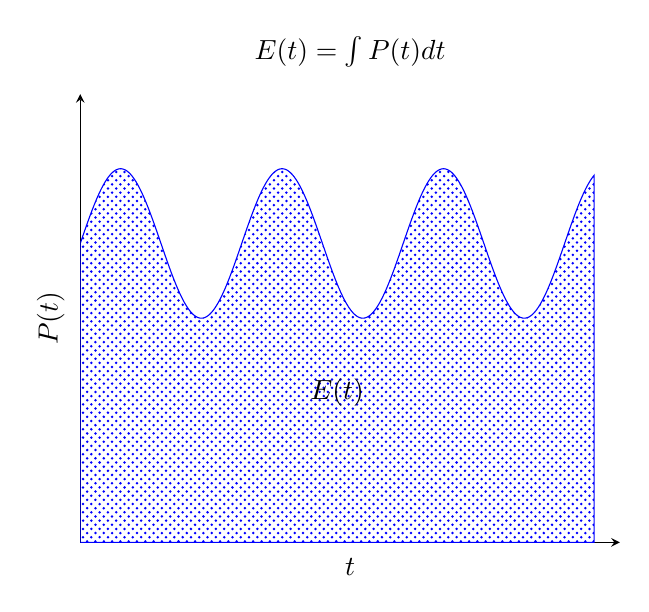
\begin{tikzpicture}
        \begin{axis}[
          title={$E(t)=\int P(t) dt$},
          ymin=0,
          ymax=3,
          xmax=21,
          domain=0:20,
          ylabel=$P(t)$,
          xlabel=$t$,
          xtick=\empty,
          ytick=\empty,
          axis x line=left,
          axis y line=left,
          ]

          % \addplot[const plot, blue,fill=blue,smooth,
          % ] plot coordinates
          % {(0,4)(1,2)(2,6)(3,4)(4,4)};


          \addplot[pattern=crosshatch dots, pattern
          color=blue,draw=blue, samples=500] {2+sin(deg(x))/2} \closedcycle;



          \node at (axis cs:10,1) {$E(t)$};


     \end{axis}
      \end{tikzpicture}  

      \caption{Relació entre l'energia i la potència o la quantitat
        comptada i la velocitat}
  \label{fig:multiresolucio:energia-potencia}
\end{figure}




Així doncs, la definició del problema és la següent.  Sigui $E(t)$
l'energia d'un senyal i $P(t)$ la potència instantània del senyal, es
compleix la relació $E(t)=\int P(t) dt$, la qual es mostra a la
\autoref{fig:multiresolucio:energia-potencia}. Aquesta és la mateixa
relació $Q(t)=\int v(t) dt$ en altres termes de comptador on $Q$ és la
quantitat comptada i $v$ és la velocitat instantània, o la mateixa per
a un cas discret $\Delta Q = \bar{v} \Delta t$ on $\bar{v}$ és la
velocitat mitjana mesurada durant $\Delta t$. %
  %Potser el cas discret hauria de ser $\Delta Q = \sum \bar{v}_k \Delta t_k$
Siguin $[t_a,t_b]$ i $[t_b,t_c]$ dos intervals de temps de mesura, un
comptador mesura exactament el valor de $E_{t_a}^{t_b} =
\int_{t_a}^{t_b} P(t) dt$ i de $E_{t_b}^{t_c} =\int_{t_b}^{t_c} P(t) dt$. En canvi,
un aparell de mesura de potència instantània es capaç de mesurar
exactament $P(t_a)$, $P(t_b)$ i $P(t_c)$. Ara bé, a partir del
comptador no es poden deduir exactament $P(t_a)$, $P(t_b)$ ni $P(t_c)$
i a partir de la mesura de la potència instantània no es poden deduir
exactament $\int_{t_a}^{t_b} P(t)$ ni $\int_{t_b}^{t_c} P(t)$. Tampoc
a partir del comptador es poden deduir exactament energies que no
s'han mesurat, per exemple ni $\int_{(t_a+t_b)/2}^{t_b} P(t)$ ni
$\int_{(t_a+t_b)/2}^{t_c} P(t)$; ara bé sí que serà exacte el càlcul
$\int_{t_a}^{t_b} P(t)+\int_{t_b}^{t_c} P(t)$.
  

La multiresolució és capaç de conservar aquesta exactitud del
comptatge total.  El comptatge total es pot conservar en un esquema de
multiresolució amb funcions d'agregació per atributs de suma de totals
o bé per atributs de mitjana de la funció. Aquests darrers són els que
permeten, a més, expressar la sèrie temporal resultant de la
multiresolució de forma més coherent amb l'original
(\seeref{sec:sgst:tretssemantics}). Reprenent
l'\autoref{ex:multiresolucio:f=op}, avaluem els atributs de mitjana de
la funció, els quals són semblants als atributs de total però
considerant la sèrie temporal en la representació contínua:
  
  \begin{itemize}


  \item Mitjana de la funció: $f_0=\operatorname{mitjana}$, segons el
    patró general de mitjana de la funció mostrat a
    \textref{sec:sgstm:mitjanafuncio}, el qual es correspon a calcular
    la mitjana de la funció de representació de la sèrie temporal
    $\frac{1}{b-a} \int_{a}^{b} S(t)dt$ en l'interval tancat $[a,b]$.

    Sigui $t_M=T(\max(S))$ i $t_m=T(\min(S))$ i $S'= \{
    (\tau_0+\delta_0, \frac{1}{\delta_0}
    \int_{\tau_0}^{\tau_0+\delta_0} S(t) dt), (\tau_0+2\delta_0,
     \frac{1}{\delta_0}\int_{\tau_0+\delta_0}^{\tau_0+2\delta_0} S(t) dt), \dotsc,
    (\tau_0+M\delta_0, \frac{1}{\delta_0}
    \int_{\tau_0+(M-1)\delta_0}^{\tau_0+M\delta_0} S(t) dt )\}$, on
    s'ha aplicat $\delta_0= (\tau_0+\delta_0)-(\tau_0)=\dotsb=
    (\tau_0+M\delta_0)-(\tau_0+(M-1)\delta_0)$.  Els resultats que cal
    calcular són $r_1=\frac{1}{t_M-t_m} \int_{t_m}^{t_M} S(t)dt$ i
    $r_2 = \frac{1}{t_M-t_m} \int_{t_m}^{t_M} S'(t)$.

    Si suposem $\tau_0=t_m$ i $\tau_0+M\delta_0=t_M$ aleshores
    $\int_{t_m}^{t_M} S'(t) = \int_{\tau_0}^{\tau_0+\delta_0} S'(t) dt + \int_{\tau_0+\delta_0}^{\tau_0+2\delta_0} S'(t) dt + \dotsb + \int_{\tau_0+(M-1)\delta_0}^{\tau_0+M\delta_0}
    S'(t) dt$.  
    
    Si resolem per exemple el primer interval de consolidació: $
    \int_{\tau_0}^{\tau_0+\delta_0} S'(t) dt = \delta_0V(m'_0) =
    \delta_0 \frac{ \int_{\tau_0}^{\tau_0+\delta_0} S(t)
      dt}{\delta_0}$ on $m'_0$ és la mesura corresponent a la
    consolidació en el primer interval. Així doncs
    $\int_{\tau_0}^{\tau_0+\delta_0} S'(t) dt =
    \int_{\tau_0}^{\tau_0+\delta_0} S(t) dt$, de fet és la propietat
    que resumeix la mitjana de la funció, i per tant podem estendre-ho
    a $\int_{t_m}^{t_M} S'(t)= \int_{t_m}^{t_M} S(t)$. Podem
    concloure, doncs, que $r_1=r_2$.


    A la \autoref{fig:multiresolucio:comptador} es mostra un exemple
    amb valors concrets on $S=\{ (1,4),(2,2),(3,6),(4,4)\}$ i
    l'esquema de multiresolució és
    $e=\{(\delta_0=2,f_0=\glssymbol{not:sgstm:meanzohe},\tau_0=0,k_0=\infty)\}$,
    segons la $\glssymbol{not:sgstm:meanzohe}$ de la
    \textref{def:sgstm:meanzohe}. La sèrie resultant de la
    consolidació de la multiresolució és $S'=\{ (2,3),(4,5)\}$. A la
    figura, les sèries temporals es representen amb representació
    \gls{zohe}, la superfície pintada en blau correspon a l'àrea de
    sota la corba de la sèrie temporal i els nombres interiors
    indiquen el valor d'aquesta àrea; en la sèrie temporal $S$ les
    àrees es corresponen amb els valors de la sèrie temporal perquè
    els intervals són d'una unitat de temps. Així doncs es pot
    observar a $S'$ com aquest esquema de multiresolució conserva el
    comptatge total en la nova resolució, és a dir $6=4+2$ en el
    primer interval consolidat i $10=6+4$ en el segon, i en una
    consulta del comptatge total per a tot l'interval $[0,4]$ s'obté
    $16$ tant en $S$ com a $S'$. Aquesta és la idea bàsica de
    conservació d'informació en els comptadors.



\begin{figure}[tp]
  \centering


     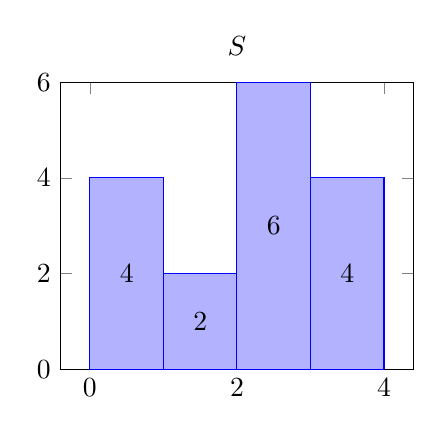
\begin{tikzpicture}
        \begin{axis}[
          width=0.5*\textwidth,
          title=$S$,
          ymin = 0,
          ymax=6,
          ]
          \addplot[
          ybar interval, 
          blue,fill=blue!30!white,
          ] plot coordinates
          {(0,4)(1,2)(2,6)(3,4)(4,4)};


    \node at (axis cs:0.5,2) {$4$};
    \node at (axis cs:1.5,1) {$2$};
    \node at (axis cs:2.5,3) {$6$};
    \node at (axis cs:3.5,2) {$4$};


     \end{axis}
      \end{tikzpicture}\qquad
     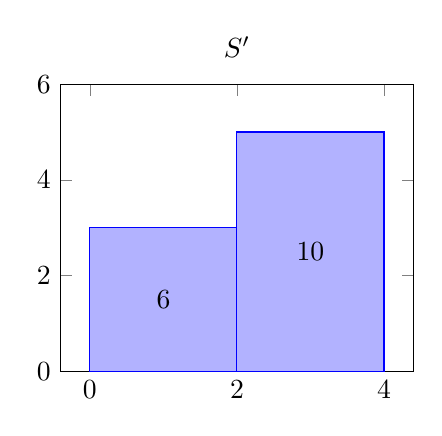
\begin{tikzpicture}
        \begin{axis}[
          width=0.5*\textwidth,
          title=$S'$,
          ymin = 0,
          ymax=6,
          ]

          \addplot[
          ybar interval, 
          blue,fill=blue!30!white,
          ] plot coordinates
          {(0,3)(2,5)(4,5)};

    \node at (axis cs:1,1.5) {$6$};
    \node at (axis cs:3,2.5) {$10$};


     \end{axis}
      \end{tikzpicture}


      \caption{Sèrie temporal amb àrea sota la corba i sèrie temporal
        resultant de la multiresolució amb agregació mitjana de la
        funció}
  \label{fig:multiresolucio:comptador}
\end{figure}






  \end{itemize}
  


La multiresolució, però, no pot conservar la resolució del comptatge,
així en l'exemple un cop s'ha consolidat $6=4+2$ no es pot tornar a
obtenir $4$ i $2$ llevat que es pogués reconstruir el senyal.  Com
s'ha exposat a
l'\autoref{ex:multireoslucio:informacio-subresolucions}, en consultes
en què l'interval no es correspongui amb les resolucions
emmagatzemades, els totals no seran els correctes que s'obtindrien de
calcular amb les dades originals.  De fet, és el mateix problema que
hem exposat que a partir d'un comptador no es poden deduir exactament
energies que no s'han mesurat.




% \todo{potser fer un exemple on es vegi com la multiresolució pot solucionar un problema d'inframostreig en els comptadors}




\subsection{Equivalències en l'agregació d'atributs}

Hi ha casos en què és el mateix aplicar una funció d'agregació
d'atributs que aplicar-ne una altra. En aquest apartat particularment
estudiem el cas de la $\glssymbol{not:sgstm:mitjanapd}$
(\seeref{def:sgstm:mitjanapd}) i el de la
$\glssymbol{not:sgstm:meanzohe}$ (\seeref{def:sgstm:meanzohe})
per a sèries temporals regulars.

Sigui $S=\{m_0,\dotsc,m_k\}$, on $m_k=(t_k,v_k)$, una sèrie temporal
regular de període $d$ (\seeref{def:st:regular}) i sigui $[t_a,t_b]$
un interval de temps on $t_a=T(\min(S))-d=t_0-d$ i
$t_b=T(\max(S))=t_k$.  Demostrem que
$\glssymbol{not:sgstm:meanzohe}(S,[t_a,t_b]) =
\glssymbol{not:sgstm:mitjanapd}(S,[t_a,t_b])$ pel que fa al valor
resultant calculat negligint el temps resultant. És a dir en realitat demostrem
$V(\glssymbol{not:sgstm:meanzohe}(S,[t_a,t_b])) =
V(\glssymbol{not:sgstm:mitjanapd}(S,[t_a,t_b]))$ però no escrivim la
projecció de l'atribut de valor, $V()$, per a no complicar la notació.

La mitjana aritmètica de la sèrie temporal és
$\glssymbol{not:sgstm:mitjanapd}(S,[t_a,t_b])=\frac{v_0+\dotsb+v_k}{|S|}$.
%
La mitjana amb representació \gls{zohe} és
$\glssymbol{not:sgstm:meanzohe}(S,[t_a,t_b])= \frac{1}{t_b-t_a} (
v_0(t_0-t_a)+v_1(t_1-t_0)+\dotsb+ v_k(t_k-t_{k-1}) )$.

Per ser regular, $t_1-t_0 = \dotsb = t_k-t_{k-1} = d$. A més
$t_a=t_0-d$ i per tant $t_0-t_a = d$. També per ser regular, $t_k-t_0=
t_k +(- t_{k-1} + t_{k-1}) + \dotsb + (- t_1 + t_1) - t_0 = (|S|-1)d$
i per tant $t_b-t_a=t_k - (t_0 - d) = (|S|-1)d +d = |S|d$.

Reescrivint, $\glssymbol{not:sgstm:meanzohe}(S,[t_a,t_b])=
\frac{1}{|S|d} ( v_0d+v_1d+\dotsb+ v_kd ) = \frac{1}{|S|} (
v_0+v_1+\dotsb+ v_k ) = \glssymbol{not:sgstm:mitjanapd}(S,[t_a,t_b])$.



Així doncs, en una sèrie temporal regular es pot aplicar la
$\glssymbol{not:sgstm:mitjanapd}$ com a equivalent a la
$\glssymbol{not:sgstm:meanzohe}$; de fet la
\autoref{fig:multiresolucio:comptador} n'és un exemple. Un àmbit
d'aplicació d'aquestes equivalències pot ser el de simplificar els
càlculs en les consultes als \gls{SGSTM}, en els discs dels quals les
subsèries temporals normalment s'emmagatzemen regulars.
 








%%% Local Variables:
%%% TeX-master: "main"
%%% End:


%  LocalWords:  multiresolució



\part{Experimentació}
%-- Implementacions --

%\part{Experimentació}


\chapter{Introducció a les implementacions}
\label{sec:implementacions}

En aquest capítol implementem \glspl{SGST} i \glspl{SGSTM} segons els
models definits.



Idealment, en un \gls{SGBD} l'usuari executa una consulta i
l'optimitzador s'encarrega d'executar les operacions físiques més
eficients, en aquest sentit el model relacional permet trobar
expressions equivalents donada una determinada consulta. Això no
obstant, i com s'ha detallat en \textref{sec:art:sgbd}, una
implementació de \gls{SGBD} no pot abastar i ser eficient en tots els
àmbits i contextos. Així doncs, no és tan senzill mantenir totalment
la independència entre l'usuari i la implementació ja que cal que
aquest decideixi un \gls{SGBD} adequat per a cada context i fins i tot
que declari com resoldre algunes operacions.  Ara bé, és possible
mantenir la independència del nivell lògic respecte a les
implementacions, i és en aquest sentit que a continuació avaluem
diferents implementacions per als models definits de \gls{SGST} i de
\gls{SGSTM}, on cada implementació està pensada per a un context
determinat.


Anomenem de forma diferent cada implementació que dissenyem per tal de
distingir-les clarament. Són les següents:

\begin{itemize}
\item Pytsms i RoundRobinson: Implementacions a alt nivell per a
  observar el funcionament a nivell acadèmic, amb llenguatge
  Python. Aquesta és la nostra implementació de referència per als
  models de \gls{SGST} i \gls{SGSTM}, la qual a més usem per als
  experiments amb dades.

\item RoundRobindoop: Implementació específica per a la resolució en
  diferit i amb computació para\.lela de la multiresolució, amb model
  de programació MapReduce i en el sistema de computació distribuïda
  Hadoop.

\item Reltsms: Implementació a alt nivell en un \gls{SGBDR}, amb
  llenguatge Tutorial~D i en el sistema Rel.

% \item RoundRobinhard: Implementació a baix nivell d'estructures
%   específiques, amb disseny de circuits digitals o amb llenguatge
%   VHDL. \todo{aquesta va en un apèndix?}


%S'avaluen implementacions específiques com RRDtool?

\end{itemize}

Finalment, en un exemple complet s'experimenta amb les implementacions
amb dades reals. Les implementacions són de programari lliure i els
codis font es poden trobar a \cite{llusa:implementacions}.










\section{Particularitats de les implementacions}



Els models d'implementacions pertanyen al nivell físic dels \gls{SGBD}
i són una realització d'un model lògic, en el nostre cas dels models
lògics de \gls{SGST} i de \gls{SGSTM}. Per a les implementacions se
sol definir el nivell d'usuari, que és el llenguatge que serà visible
per als usuaris. Les implementacions que realitzem volen ser molt
properes al model lògic i per tant el nivell d'usuari que se'n deriva
és molt similar. Per a ser un llenguatge d'usuari complet es
requereixen facilitats i capacitats de llenguatge de programació
--bucles, condicionals, declarar variables, etc.-- per a la qual
cosa ens basem en els recursos particulars de cada implementació:
Python, Tutorial~D, etc. L'objectiu principal, però, d'aquestes
implementacions és acadèmic i per tant no considerem prioritari el
llenguatge d'usuari.

% Aquestes facilitats en el nivell lògic no s'expliciten ja que es
% consideren inherents a les matemàtiques.



En la implementació s'afegeixen alguns operadors que en el model
estructural no havíem definit explícitament perquè ja són propis de
l'àlgebra de conjunts. Així per exemple, alguns d'aquests operadors
que s'han d'implementar són els relacionats amb la notació de creació
de conjunts, %set-builder notation (set comprehension)
els quals en els \gls{SGBD} s'inclouen en el que es coneix com a
\gls{DDL}, o els relacionats amb la manipulació de les dades amb
assignació, inserció, modificació o esborrament, els quals en els
\gls{SGBD} es coneixen com a \gls{DML}.  En el cas dels \gls{SGSTM} sí
que hem definit en el model algunes operacions de \gls{DDL} i \gls{DML} per a
l'esquema multiresolució, ja que aquest requereix ser manipulat
coherentment.

% Pel que fa al llenguatge de consultes (\emph{query language}),
% s'implementa seguint el model d'operacions de consulta de cada cas.





\section{Qüestions de format}

% Llistat: Resultat d’operacions efectuades per un ordinador, escrit en paper per una impressora. en l'àmbit de l'electrònica/informàtica


En els capítols següents s'utilitzen llistats per a mostrar exemples
de funcionament i els resultats de les operacions efectuades.  El
format dels llistats depèn del tipus d'informació que mostren. Així,
bàsicament, els exemples de codi tenen fons gris, com el
\autoref{lst:format:python}, i els exemples de fitxers o sortides per
pantalla tenen fons groc, com el \autoref{lst:format:stdout}.



\begin{lstlisting}[style=py,caption=Exemple de codi,label=lst:format:python]
>>> from pytsms import TimeSeries, Measure as m

>>> s = TimeSeries([m(1,6),m(5,2),m(8,5),m(10,0),m(14,1),m(19,6),m(22,11),m(26,6),m(29,0)])
\end{lstlisting}



\begin{lstlisting}[style=stdout,caption=Exemple de fitxer o de sortida per pantalla,label=lst:format:stdout]
10/maximum_zohe-10	10 0.0
10/maximum_zohe-10	14 1.0
\end{lstlisting}




%%% Local Variables:
%%% TeX-master: "main"
%%% End:




\chapter{Python}


La implementació de referència dels models de SGST i SGSTM s'ha
realitzat amb Python \todo{referència}. L'objectiu d'aquesta
implementació de referència és mantenir la fidelitat al model per tal
de poder experimentar-hi amb tota la potència matemàtica .

En la implementació s'han afegit alguns operadors que en el model ja
estaven definits perquè són propis de l'àlgebra de conjunts. Alguns
dels operadors principals que s'han d'afegir són els relacionats amb
la notació de creació de conjunts, els quals en els SGBD es coneixen
com a \emph{llenguatge de definició de dades} (DDL, de l'anglès
\emph{data definition language}). 


Implementem els dos models de SGST i SGSTM com a dues biblioteques
diferents: \emph{Pytsms} i \emph{RoundRobinson} respectivament. La
RoundRobinson, però, té una forta dependència en la
Pytsms de la mateixa manera que hem definit els SGSTM en base
als SGST.


Utilitzem orientació a objectes. Ens permet fer explicita la relació
entre la implementació i el model. \todo{més explicat}

Utilitzem diagrames UML per a definir l'estructura de classes. \todo{més explicat}


Implementem la part essencial, és a dir l'àlgebra definida en els
models lògics. No implementem els complements habituals dels SGBD, els
quals són necessaris en entorns d'explotació, com per exemple gestió
d'usuaris i permisos, còpies de seguretat, llenguatges estàndards de
consulta, etc.




\section{Pytsms}

La biblioteca Pytsms implementa un SGST de referència. Així
doncs, seguint el model, els objectes principals són les mesures, les
sèries temporals i les representacions de les sèries temporals. Tots
tres s'implementen respectivament com a classes \emph{Measure},
\emph{TimeSeries} i \emph{Representation}.


\begin{figure}[tp]
  \centering
  \begin{tikzpicture}

  %Timeseries
  \umlclass[x=0,y=0] {TimeSeries}{}{}  

  % Measure
  \umlclass[x=-4] {Measure}{}{}
  \umluniaggreg[mult=0..*]  {TimeSeries}{Measure}
  \umlclass[x=-5.2,y=-2] {MFloat}{}{}
  \umlclass[x=-2.8,y=-2] {MChar}{}{}
  \umlinherit {MFloat}{Measure}
  \umlinherit {MChar}{Measure}

  %Repr
  \umlclass[x=4] {Representation}{}{} %,type=abstract
  \umlassoc[mult1=1,mult2=1]  {TimeSeries}{Representation}
  \umlclass[x=3,y=-2] {Zohe}{}{}
  \umlclass[x=5,y=-2] {Partial}{}{}
  \umlinherit {Zohe}{Representation}
  \umlinherit {Partial}{Representation}

  %Associacions
  \umlclass[x=-1.5,y=-4] {RegularProp}{}{}
  \umluniassoc  {RegularProp}{TimeSeries}
  \umlclass[x=1.5,y=-4] {Storage}{}{}
  \umluniassoc {Storage}{TimeSeries}
  \end{tikzpicture}


  \caption{Diagrama UML de Pytsms}
  \label{fig:implementacio:pytsms-uml}
\end{figure}


\begin{figure}
  \centering

\begin{tikzpicture}

  %Timeseries
  \umlclass[x=0,y=0] {TimeSeries}{}{}  
  %Realisations 
  \umlclass[x=-3.5,y=-3] {Structure}{}{}
  \umlclass[x=-1.2,y=-3] {OpSet}{}{}
  \umlclass[x=1.2,y=-3] {OpSeq}{}{}
  \umlclass[x=3.5,y=-3] {OpFunc}{}{}
  %\umlreal[geometry=|-|]{Structure}{TimeSeries}
  \umlinherit[geometry=|-|]{TimeSeries}{Structure}
  \umlinherit[geometry=|-|]{TimeSeries}{OpSet}
  \umlinherit[geometry=|-|]{TimeSeries}{OpSeq}
  \umlinherit[geometry=|-|]{TimeSeries}{OpFunc}
  %Subrealisations
  \umlclass[x=-3,y=-6] {SetNoTemporal}{}{}
  \umlclass[x=0.7,y=-6] {SetTemporal}{}{}
  \umlclass[x=4,y=-6] {SetRelacional}{}{}
  \umlinherit[geometry=|-|]{OpSet}{SetNoTemporal}
  \umlinherit[geometry=|-|]{OpSet}{SetTemporal}
  \umlinherit[geometry=|-|]{OpSet}{SetRelacional}
  \umlclass[x=-6,y=-6] {Set}{}{}
  \umlinherit{Structure}{Set}

\end{tikzpicture}

  \caption{Diagrama UML de la realització de sèries temporals a Pytsms}
  \label{fig:implementacio:pytsms-uml-ts}
\end{figure}





La \autoref{fig:implementacio:pytsms-uml} mostra amb un diagrama
UML la relació entre aquests tres objectes principals. Així, per una
banda, una \emph{TimeSeries} té una relació d'agregació amb les
\emph{Measure}, és a dir que una sèrie temporal conté cap, una o més
d'una mesura.  Per altra banda, les sèries temporals i les
representacions són ortogonals i això s'implementa mitjançant una
relació d'associació bidireccional entre una \emph{TimeSeries} i una
\emph{Representation}, és a dir que una instància de sèrie temporal té
associada una representació i una instància de representació coneix la
sèrie temporal que representa.




Una \emph{TimeSeries} és un objecte amb una gran quantitat de
mètodes. Com a conseqüència, la implementació de funcionalitats
essencials s'ha dividit en diversos mòduls, el qual es mostra a la
\autoref{fig:implementacio:pytsms-uml-ts}. Els mètodes que implementen
el model estructural i el model d'operacions bàsiques s'han agrupat en
objectes segons la seva funcionalitat. Així hi ha l'objecte
\emph{Structure} que implementa el model estructural de les sèries
temporals, l'\emph{OpSet} pel model d'operacions de conjunts,
l'\emph{OpSeq} pel model d'operacions de seqüències i l'\emph{OpFunc}
pel model d'operacions de funció temporal.  Aleshores el
\emph{TimeSeries} hereta les funcionalitats d'aquests quatre objectes.
L'objecte \emph{OpSet} també té una gran quantitat de mètodes i, de la
mateixa manera, hereta la funcionalitat de tres objectes: el
\emph{SetNoTemporal} per les operacions basades en l'orde parcial de
les sèries temporals, el \emph{SetTemporal} basat en l'ordre temporal
i el \emph{SetRelacional} per les operacions específiques de l'àlgebra
relacional. Pel que fa a l'\emph{Structure} hereta funcionalitats dels
objectes \emph{Set}, que són un tipus predefinit a Python.


Les funcionalitats complementàries de les \emph{TimeSeries} s'han
implementat amb relacions d'associació unidireccionals, el qual es
mostra a la \autoref{fig:implementacio:pytsms-uml}. Així, hi ha dues
funcionalitats complementàries: \emph{RegularProperties} per a les
operacions relacionades amb la regularitat de les sèries temporals i
\emph{Storage} per a operacions d'emmagatzematge i de recuperació en
fitxers. Ens aquest cas, l'associació unidireccional indica que són
objectes que treballen sobre una \emph{TimeSeries}.





La \autoref{fig:implementacio:pytsms-uml} mostra
especialitzacions de les mesures i de les representacions.

Pel que fa a les \emph{Measure}, poden tenir especialitzacions segons
els tipus dels atributs de temps i de valor. Amb aquesta relació
implementem la propietat homogènia de les sèries temporals i la
definició de mesura indefinida i de valor indefinit, és a dir que
totes les mesures que conté una sèrie temporal són del mateix tipus i
cada tipus de mesura té uns valors de l'atribut temps que la
defineixen indefinida i uns valors de l'atribut valor que la
defineixen de valor indefinit.  Així, per defecte, una \emph{Measure}
defineix els reals $-\infty$ i $+\infty$ per a les mesures indefinida
negativa i positiva respectivament, i defineix el valor \emph{None} de
Python per a la mesura de valor indefinit. Aleshores, mitjançant
especialitzacions es poden definir altres tipus de mesures; per
exemple la \emph{MFloat} que defineix el real $\infty$ com a valor
indefinit o bé la \emph{MChar} que defineix mesures de tipus caràcter.





Pel que fa a les representacions, cada representació en concret és una
especialització de \emph{Representation}. Per exemple \emph{Zohe} i
\emph{Partial} implementen la funció de representació ZOHE i la
discreta pura respectivament. 
%\emph{Representation} és una classe abstracta?
Bàsicament, cada representació particular ha de definir l'operació que
calcula l'interval temporal i l'operació que permet trobar-ne el graf.
També cadascuna implementa una operació que dibuixi correctament el
gràfic de la sèrie temporal segons la representació; en les
representacions d'exemple definides s'usa la biblioteca
\emph{Matplotlib} \todo{referència} per a fer els gràfics.




\subsubsection{Encaix a Python}

\todo{}

Heretem de sets, implementem els mètodes especials de sets

implementem els mètodes especials de seqüències







\section{RoundRobinson}

La biblioteca RoundRobinson implementa un SGSTM de referència. Així
doncs, seguint el model, els objectes principals són les sèries
temporals multiresolució, les subsèries resolució, els buffers, els
discs i les funcions d'agregació d'atributs.


les mesures, les
sèries temporals i les representacions de les sèries temporals. Tots
tres s'implementen respectivament com a classes \emph{Measure},
\emph{TimeSeries} i \emph{Representation}.




\begin{tikzpicture}

  %MultiTimeseries
  \umlclass[x=0,y=0] {MultiresolutionSeries}{}{}  
  \umlclass[x=4,y=0] {Set}{}{}
  \umlinherit{MultiresolutionSeries}{Set}
  %Components 
  \umlclass[x=0,y=-3] {Resolution}{}{}
  \umluniaggreg  {MultiresolutionSeries}{Resolution}
  %SubComponents 
  \umlclass[x=-1.2,y=-6] {Buffer}{}{}
  \umlclass[x=1.2,y=-6] {Disc}{}{}
  \umlclass[x=-3,y=-9] {Aggregators}{}{}
  \umlunicompo[mult=1]  {Resolution}{Buffer}
  \umlunicompo[mult=1]  {Resolution}{Disc}
  \umluniassoc[mult=1]  {Buffer}{Aggregators}

  %TimeSeries
  \begin{umlpackage}[x=0,y=-9]{pyTsms}
    \umlclass{TimeSeries}{}{}  
  \end{umlpackage}
  \umluniassoc[mult=1]  {Buffer}{TimeSeries}
  \umluniassoc[mult=1]  {Disc}{TimeSeries}

  %Associacions
  \umlclass[x=5,y=2] {Storage}{}{}
  \umluniassoc {Storage}{MultiresolutionSeries}
  \umlclass[x=2,y=2] {Plot}{}{}
  \umluniassoc {Plot}{MultiresolutionSeries}

\end{tikzpicture}




\section{Casos d'ús}


\todo{}


Amb les biblioteques Pytsms i RoundRobinson podem treballar amb les sèries temporals i les sèries temporals multiresolució. 


Alguns cas d'exemple és demostrar l'equivalència entre l'operació multiresolució dels SGST sobre una sèrie temporal i la sèrie temporal resultant d'una consolidació dels SGSTM. 












%%% Local Variables:
%%% TeX-master: "main"
%%% End:
\chapter{Implementació amb para\l.lelisme}
\label{sec:implementacio:mapreduce}


\todo{alerta que s'han canviar els noms de mapa i plec de multiresolució}
\todo{alerta en el canvi de rrdoop al reduce: ara retorna delta f tab t v} 
\todo{ara es pot fer servir el LoadCsv del roundrobinson per a jugar amb el resultat: documentar-ho i també documentar el LoadCsv a roundrobinson}

En el capítol \todo{ref al capítol} hem definit la funció de
multiresolució com una funció sobre una sèrie temporal. Aquesta funció
té bàsicament dues parts: un plec sobre un esquema de multiresolució i
mapes sobre la sèrie temporal. Ara implementem
aquesta funció mitjançant computació para\l.lela.


Una tècnica de computació para\l.lela és
MapReduce \parencite{deanghemawat04:mapreduce}, la qual s'adequa bé al
problema ja que es basa en aplicar operacions de mapa (\emph{map}) i
posteriorment plegar-les (\emph{reduce}). Un sistema que es basa
exclusivament en aquesta tècnica és
Hadoop \parencite{hadoop}.

A continuació, en primer lloc, estudiem Hadoop i la tècnica MapReduce.
En segon lloc, implementem usant Hadoop un \gls{SGSTM} anomenat
\emph{RoundRobindoop}. Aquest és un \gls{SGSTM} específic amb
l'objectiu de mostrar una implementació que resolgui la multiresolució
d'una sèrie temporal en temps diferit (\emph{offline}) i computant
para\l.lelament.




\section{Hadoop i MapReduce}


Apache Hadoop, o simplement Hadoop, \parencite{hadoop} és un sistema
de computació distribuïda que permet processar grans volums de dades
amb diferents computadors en para\l.lel. El sistema inclou la gestió
de l'emmagatzematge per a distribuir les dades als diferents
computadors, la qual cosa s'anomena \gls{HDFS}; la gestió dels
diferents processos en els diversos computadors; i el model de
programació para\l.lela, el qual és MapReduce.


MapReduce \parencite{deanghemawat04:mapreduce,lammel08:mapreduce} és
un model de programació per processar algoritmes en para\l.lel. Es
basa en resoldre els algoritmes en dues etapes: primer en una etapa de
\emph{maps} i segon en una etapa de \emph{reduces}.  Aquestes dues
etapes són l'algoritme bàsic i per això s'anomena MapReduce, tot i que
hi ha variacions que afegeixen més etapes.  Els noms de \emph{map} i
\emph{reduce} també s'usen per a les operacions d'alt ordre, com les
mapa (\emph{map}) i plec (\emph{fold} o també \emph{reduce}), que hem
definit en el model dels \gls{SGST}, però
\textcite{lammel08:mapreduce} compara les de MapReduce amb les d'alt
ordre i conclou que no són exactament el mateix; aquí distingirem els
conceptes usant els noms en anglès map i reduce per a MapReduce.


A la~\autoref{fig:mapreduce:esquema}
es mostra l'esquema de funcionament de MapReduce, que és el següent:


\begin{figure}[tp]
  \centering
  \chapter{Implementació amb para\l.lelisme}
\label{sec:implementacio:mapreduce}


\todo{alerta que s'han canviar els noms de mapa i plec de multiresolució}
\todo{alerta en el canvi de rrdoop al reduce: ara retorna delta f tab t v} 
\todo{ara es pot fer servir el LoadCsv del roundrobinson per a jugar amb el resultat: documentar-ho i també documentar el LoadCsv a roundrobinson}

En el capítol \todo{ref al capítol} hem definit la funció de
multiresolució com una funció sobre una sèrie temporal. Aquesta funció
té bàsicament dues parts: un plec sobre un esquema de multiresolució i
mapes sobre la sèrie temporal. Ara implementem
aquesta funció mitjançant computació para\l.lela.


Una tècnica de computació para\l.lela és
MapReduce \parencite{deanghemawat04:mapreduce}, la qual s'adequa bé al
problema ja que es basa en aplicar operacions de mapa (\emph{map}) i
posteriorment plegar-les (\emph{reduce}). Un sistema que es basa
exclusivament en aquesta tècnica és
Hadoop \parencite{hadoop}.

A continuació, en primer lloc, estudiem Hadoop i la tècnica MapReduce.
En segon lloc, implementem usant Hadoop un \gls{SGSTM} anomenat
\emph{RoundRobindoop}. Aquest és un \gls{SGSTM} específic amb
l'objectiu de mostrar una implementació que resolgui la multiresolució
d'una sèrie temporal en temps diferit (\emph{offline}) i computant
para\l.lelament.




\section{Hadoop i MapReduce}


Apache Hadoop, o simplement Hadoop, \parencite{hadoop} és un sistema
de computació distribuïda que permet processar grans volums de dades
amb diferents computadors en para\l.lel. El sistema inclou la gestió
de l'emmagatzematge per a distribuir les dades als diferents
computadors, la qual cosa s'anomena \gls{HDFS}; la gestió dels
diferents processos en els diversos computadors; i el model de
programació para\l.lela, el qual és MapReduce.


MapReduce \parencite{deanghemawat04:mapreduce,lammel08:mapreduce} és
un model de programació per processar algoritmes en para\l.lel. Es
basa en resoldre els algoritmes en dues etapes: primer en una etapa de
\emph{maps} i segon en una etapa de \emph{reduces}.  Aquestes dues
etapes són l'algoritme bàsic i per això s'anomena MapReduce, tot i que
hi ha variacions que afegeixen més etapes.  Els noms de \emph{map} i
\emph{reduce} també s'usen per a les operacions d'alt ordre, com les
mapa (\emph{map}) i plec (\emph{fold} o també \emph{reduce}), que hem
definit en el model dels \gls{SGST}, però
\textcite{lammel08:mapreduce} compara les de MapReduce amb les d'alt
ordre i conclou que no són exactament el mateix; aquí distingirem els
conceptes usant els noms en anglès map i reduce per a MapReduce.


A la~\autoref{fig:mapreduce:esquema}
es mostra l'esquema de funcionament de MapReduce, que és el següent:


\begin{figure}[tp]
  \centering
  \chapter{Implementació amb para\l.lelisme}
\label{sec:implementacio:mapreduce}


\todo{alerta que s'han canviar els noms de mapa i plec de multiresolució}
\todo{alerta en el canvi de rrdoop al reduce: ara retorna delta f tab t v} 
\todo{ara es pot fer servir el LoadCsv del roundrobinson per a jugar amb el resultat: documentar-ho i també documentar el LoadCsv a roundrobinson}

En el capítol \todo{ref al capítol} hem definit la funció de
multiresolució com una funció sobre una sèrie temporal. Aquesta funció
té bàsicament dues parts: un plec sobre un esquema de multiresolució i
mapes sobre la sèrie temporal. Ara implementem
aquesta funció mitjançant computació para\l.lela.


Una tècnica de computació para\l.lela és
MapReduce \parencite{deanghemawat04:mapreduce}, la qual s'adequa bé al
problema ja que es basa en aplicar operacions de mapa (\emph{map}) i
posteriorment plegar-les (\emph{reduce}). Un sistema que es basa
exclusivament en aquesta tècnica és
Hadoop \parencite{hadoop}.

A continuació, en primer lloc, estudiem Hadoop i la tècnica MapReduce.
En segon lloc, implementem usant Hadoop un \gls{SGSTM} anomenat
\emph{RoundRobindoop}. Aquest és un \gls{SGSTM} específic amb
l'objectiu de mostrar una implementació que resolgui la multiresolució
d'una sèrie temporal en temps diferit (\emph{offline}) i computant
para\l.lelament.




\section{Hadoop i MapReduce}


Apache Hadoop, o simplement Hadoop, \parencite{hadoop} és un sistema
de computació distribuïda que permet processar grans volums de dades
amb diferents computadors en para\l.lel. El sistema inclou la gestió
de l'emmagatzematge per a distribuir les dades als diferents
computadors, la qual cosa s'anomena \gls{HDFS}; la gestió dels
diferents processos en els diversos computadors; i el model de
programació para\l.lela, el qual és MapReduce.


MapReduce \parencite{deanghemawat04:mapreduce,lammel08:mapreduce} és
un model de programació per processar algoritmes en para\l.lel. Es
basa en resoldre els algoritmes en dues etapes: primer en una etapa de
\emph{maps} i segon en una etapa de \emph{reduces}.  Aquestes dues
etapes són l'algoritme bàsic i per això s'anomena MapReduce, tot i que
hi ha variacions que afegeixen més etapes.  Els noms de \emph{map} i
\emph{reduce} també s'usen per a les operacions d'alt ordre, com les
mapa (\emph{map}) i plec (\emph{fold} o també \emph{reduce}), que hem
definit en el model dels \gls{SGST}, però
\textcite{lammel08:mapreduce} compara les de MapReduce amb les d'alt
ordre i conclou que no són exactament el mateix; aquí distingirem els
conceptes usant els noms en anglès map i reduce per a MapReduce.


A la~\autoref{fig:mapreduce:esquema}
es mostra l'esquema de funcionament de MapReduce, que és el següent:


\begin{figure}[tp]
  \centering
  \input{imatges/implementacio/mapreduce.tex}
  \caption{Esquema de funcionament de MapReduce}
  \label{fig:mapreduce:esquema}
\end{figure}



\begin{enumerate}

\item Hi ha unes dades originals que es poden partir en
  trossos. Hadoop està orientat a fitxers, mitjançant \gls{HDFS}, i
  per tant cada tros de dades és cadascun dels fitxers que es volen
  processar o bé conjunts de línies d'un fitxer.

\item Cada tros de les dades es processa mitjançant una operació
  map. Cada map es pot computar en para\l.lel i distribuït.

\item Cada operació map ha de retornar un nou conjunt de dades
  formats per parelles d'identificador i valor. Aquests conjunts de
  dades s'ordenen per identificador. 

\item Cada conjunt de dades amb el mateix identificador es processa
  mitjançant una operació reduce. Cada reduce es pot computar en
  para\l.lel i distribuït.

\item Cada reduce ha de retornar un tros del resultat final. És a dir,
  que unint les dades que retornen els reduce s'obtenen les dades
  finals. En l'orientació a fitxers de Hadoop, el resultat final és un
  fitxer, o bé un tros d'un fitxer, per a cada reduce.

\end{enumerate}



Per a resoldre un algoritme amb MapReduce, cal definir l'operació de
map i l'operació de reduce. El map ha de calcular un filtre sobre les
dades, sobretot establir grups de dades, i el reduce ha de calcular
agregacions o resums per a cada grup. MapReduce té una gran similitud
amb l'operació \emph{summarize} dels
\gls{SGBDR} \parencite[cap.~7]{date04:introduction8}, però separada
convenientment en les dues etapes.  A més, MapReduce imposa les
següents restriccions: les dades s'han de poder partir i l'algoritme
s'ha de poder expressar separat en les dues operacions de map i de
reduce.  \textcite{deanghemawat04:mapreduce} mostren exemples
d'algoritmes que es poden expressar amb MapReduce.



Un cop s'ha modelat un algoritme amb MapReduce, aleshores Hadoop ja és
capaç d'executar els maps i els reduces en para\l.lel i distribuïts. A
més, Hadoop també gestiona el compromís dels recursos entre el temps
de distribuir les dades, la quantitat de processos en para\l.lel que
s'han de crear i el temps afegit que suposa cada procés nou.








\section{RoundRobindoop}


RoundRobindoop implementa un \gls{SGSTM} específic que resol la funció
de multiresolució amb el model de programació MapReduce.  Per a
construir RoundRobindoop, primer dissenyem l'algoritme de MapReduce
que s'adequa a la multiresolució. Segon, proposem dues maneres per a
executar RoundRobindoop: amb Hadoop i la shell del sistema.



\subsection{Multiresolució amb MapReduce}

L'algoritme que implementem amb MapReduce és el de la funció de
multiresolució definida a la secció \todo{ref sec: multiresolucio: funcio}. Aquesta funció principalment té dues
parts, una de mapa i una de plec, que com ja s'ha dit no es poden
correspondre exactament amb les operacions de map i de reduce. 
 Així
doncs, dissenyem les operacions de map i de reduce que tenen el mateix
efecte que calcular la funció de multiresolució, en què el resultat
final no és la sèrie temporal total sinó el resultat de totes les
funcions $\glssymbol{not:sgstm:dmap}$, és a dir el resultat final són
les sèries temporals dels discs del model de \gls{SGSTM} la
concatenació dels quals resulta en la sèrie temporal total.



Sigui $S=\{m_0,m_1,\dotsc,m_k\}$ una sèrie temporal, i $e = \{
(\delta_0,f_0,\tau_0,k_0),\ldots, (\delta_d,f_d,\tau_d,k_d)\}$ els
paràmetres d'un esquema de multiresolució, definim l'algoritme
MapReduce que calcula $\operatorname{mapreduce}(S,e) = \{
(\delta_0,f_0,
\glssymbol{not:sgstm:dmap}(S,\delta_0,f_0,\tau_0,k_0)),\dotsc,
(\delta_c,f_c,\glssymbol{not:sgstm:dmap}(S,\delta_c,f_c,\tau_c,k_c))
\}$. És a dir, calcula tots els $\glssymbol{not:sgstm:dmap}$ possibles
i els identifica amb el pas de consolidació $\delta$ i la funció
d'agregació d'atributs $f$, els quals identifiquen les subsèries
resolució assumint que no n'hi ha de repetits.
%i que per tant tenenassociats el cardinal màxim $k$ i un instant de consolidació $\tau$.





L'esquema de funcionament de RoundRobindoop és el de
la~\autoref{fig:roundrobindoop:esquema}, el qual és la implementació
particular de l'esquema de la~\autoref{fig:mapreduce:esquema} per a la
multiresolució.  De forma resumida, RoundRobindoop en l'etapa de map
classifica les mesures en funció de a quin disc i temps resultant es
consolidaran i en l'etapa de reduce calcula la funció d'agregació per
a les mesures que s'hagin de consolidar al mateix disc.  A continuació
expliquem detalladament com són les dades originals ($O$), les
d'entremig ($E$) i les finals ($F$), i finalment definim l'operació de
map i la de reduce.





\begin{figure}[tp]
  \centering

  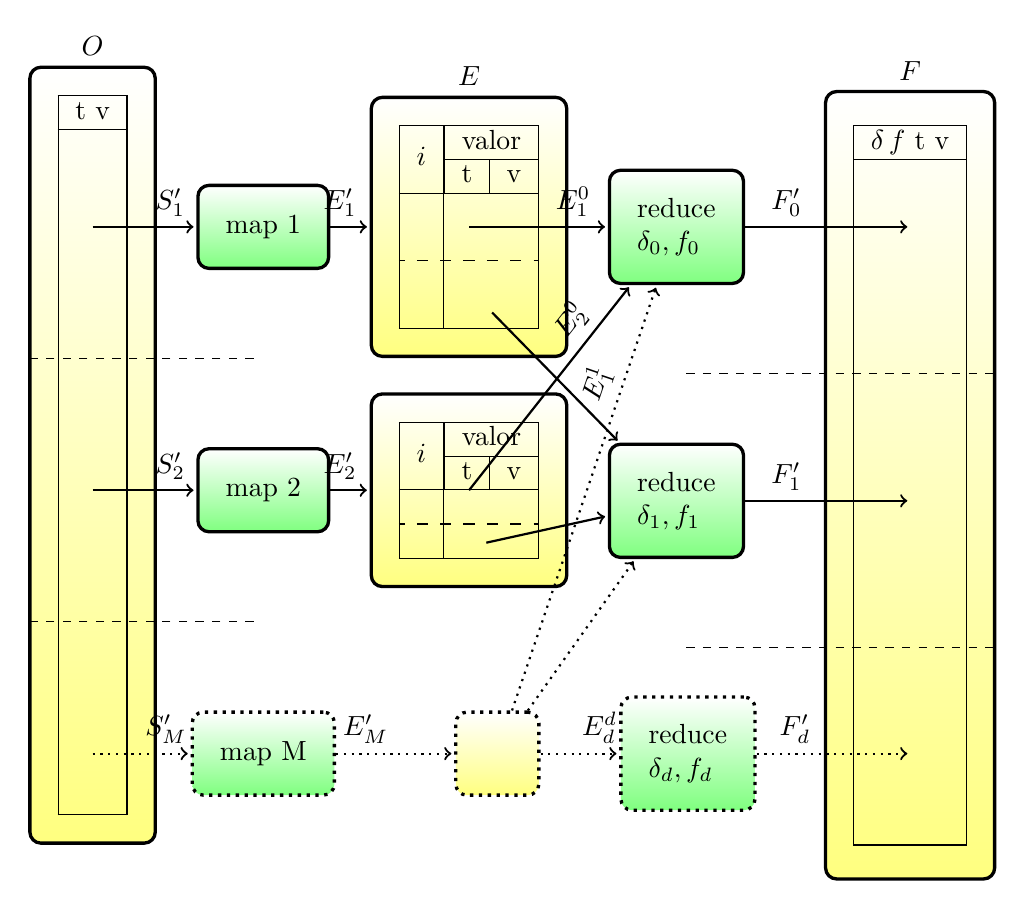
\begin{tikzpicture}

      \tikzset{
        mynode/.style={rectangle,rounded corners,draw=black, 
          very thick, inner sep=1em, minimum size=3em, text centered,
          groc},
        myarrow/.style={->, shorten >=1pt, thick},
        mylabel/.style={text width=7em, text centered},
        groc/.style={top color=white, bottom color=yellow!50},
        verd/.style={top color=white, bottom color=green!50},
        roig/.style={top color=white, bottom color=red!50},
      }  




 \node[mynode,verd] (m1) {map 1};
 \node (ml1) [below=of m1] {};
 \node[mynode,verd] (m2) [below=of ml1] {map 2};
 \node (ml2) [below=of m2] {};
 \node[mynode,verd,dotted] (mn) [below=of ml2] {map M};


 \node[mynode] (d1) [right=0.5cm of m1] {
   \begin{tabular}{|c|cc|}\hline
     \multirow{2}{*}{$i$} & \multicolumn{2}{|c|}{valor} \\\cline{2-3}
       & \multicolumn{1}{|c|}{t} & v \\\hline
      & & \\
      & &\\\hdashline
      & &\\
      & &\\\hline
   \end{tabular}
 };

 \node[mynode] (d2) [right=0.5cm of m2] {
   \begin{tabular}{|c|cc|}\hline
     \multirow{2}{*}{$i$} & \multicolumn{2}{|c|}{valor} \\\cline{2-3}
       & \multicolumn{1}{|c|}{t} & v \\\hline
      & &\\\hdashline
      & &\\\hline
   \end{tabular}
 };

 \node[mynode,dotted] (dn) [right=1.5cm of mn] {};



 \node[mynode,verd] (r1) [right=0.5cm of d1] {\parbox{1cm}{reduce $\delta_0,f_0$}};
 \node[mynode,verd] (r2) [below=2cm of r1] {\parbox{1cm}{reduce $\delta_1,f_1$}};
 \node[mynode,verd,dotted] (rn) [right=1cm of dn] {\parbox{1cm}{reduce $\delta_d,f_d$}};




 \node[mynode] (o) [above left=1.5cm and 0.5cm of m1, anchor=north east] {
   \begin{tabular}{|c|}\hline
     t v \\\hline
       \\
       \\
     \parbox[c][7cm][s]{0cm}{\vfill} \\
       \\
       \\\hline
   \end{tabular}
 };
 \node [above=0cm of o] {$O$};
 \node[mynode,minimum height=10cm] (f) [above right=of r1, anchor=north west] {
   \begin{tabular}{|c|}\hline
    $\delta\, f$ t v \\\hline
       \\
        \\
     \parbox[c][7cm][s]{0cm}{\vfill}  \\
        \\
        \\\hline
   \end{tabular}
};
 \node [above=0cm of f] {$F$};
 \node [above=0cm of d1] {$E$};




 \draw[dashed] (ml1) -- (ml1-|o.west);
 \draw[dashed] (ml2) -- (ml2-|o.west);

 \draw[myarrow] (o.center|-m1) -- (m1)  node[sloped,above,near end] {$S'_1$};
 \draw[myarrow] (o.center|-m2) -- (m2) node[sloped,above,near end] {$S'_2$};
 \draw[myarrow,dotted] (o.center|-mn) -- (mn) node[sloped,above,near end] {$S'_M$};


 \draw[myarrow] (m1) -- (d1) node[sloped,above,near start] {$E'_1$};
 \draw[myarrow] (m2) -- (d2) node[sloped,above,near start] {$E'_2$};
 \draw[myarrow,dotted] (mn) -- (dn)  node[sloped,above,near start] {$E'_M$};

 \draw[myarrow] (d1.center) -- (r1) node[sloped,above,near end] {$E_{1}^0$};
 \node (d1b) [above=3ex of d1.280] {}; 
 \draw[myarrow] (d1b.center) -- (r2) ;

 \draw[myarrow] (d2.center) -- (r1) node[sloped,above,near end] {$E_{2}^0$};
 \node (d2b) [above=3ex of d2.280] {}; 
 \draw[myarrow] (d2b.center) -- (r2) ;

 \draw[myarrow,dotted] (dn) -- (r1) node[sloped,above,near end] {$E_{1}^1$};
 \draw[myarrow,dotted] (dn) -- (r2);
 \draw[myarrow,dotted] (dn) -- (rn) node[sloped,above,near end] {$E_{d}^d$};


 \node (r1l) [below=of r1] {};
 \draw[dashed] (r1l) -- (r1l-|f.east);
 \node (r2l) [below=of r2] {};
 \draw[dashed] (r2l) -- (r2l-|f.east);


 \draw[myarrow] (r1) -- (r1-|f.center)  node[sloped,above,near start] {$F'_0$};
 \draw[myarrow] (r2) -- (r2-|f.center)  node[sloped,above,near start] {$F'_1$};
 \draw[myarrow,dotted] (rn) -- (rn-|f.center)  node[sloped,above,near start] {$F'_d$};


  \end{tikzpicture}
  
  \caption{Esquema de funcionament de RoundRobindoop}
  \label{fig:roundrobindoop:esquema}
\end{figure}






Les dades originals són la sèrie temporal $S$ és a dir un conjunt de
parelles de temps i valor, a les quals anomenem mesures. Un sèrie
temporal es pot partir en trossos on cada tros és un subconjunt de
mesures, és a dir una subsèrie temporal. Per tant, cada operació map
rep una subsèrie temporal de l'original: $S'_1 =
\{m_0,\dotsc,m_{o1}\}, S'_2 = \{m_{o1+1},\dotsc,m_{o2}\}, \dotsc, S'_M
= \{\dotsc,m_{k}\}$ on $M$ són el nombre de maps i $o_1,o_2\in
\glssymbol{not:N}$, $o_1 < o_2 < k$.



Les dades d'entremig són les sèries temporals dels buffers, és a dir
les mesures pendents de consolidar per a cada subsèrie resolució.
Així doncs, les dades d'entremig vistes com a conjunt són un conjunt
de dades pendents de consolidar $E=\{ D_{0}, \dotsc, D_t\}$ on cada
dada pendent de consolidar és un tuple $D=(i,m)$ on $i=(\delta,f,t_b)$
funciona com a identificador i $m=(t,v)$ com a valor.  És a dir, que
classifica cada mesura $m$ a quines resolucions s'han de consolidar
identificades pel pas de consolidació $\delta$, per la funció
d'agregació d'atributs $f$ i pel temps resultant de consolidació
$t_b$. Per tant, cada operació map resulta en un subconjunt de les
dades d'entremig: $E'_1=\{ (\delta_0,f_0, t_{b0}^0, t_0,v_0),
(\delta_1,f_1, t_{b1}^0, t_0,v_0), \dotsc , (\delta_d,f_d, t_{bd}^0,
t_0,v_0), (\delta_0,f_0, t_{b0}^1, t_1,v_1), \dotsc, (\delta_d,f_d,
t_{bd}^{o1}, t_{o1},v_{o1}) \}$, i $E'_2$ i $E'_M$ de manera similar.
En total, les dades d'entremig tenen un cardinal de $|E|=t+1=|e||S|$
és a dir la quantitat de resolucions de l'esquema multiplicat per la
quantitat de mesures de la sèrie temporal original.


Un cop calculades, les dades d'entremig $E$ s'ordenen i
s'agrupen per identificadors $(\delta,f, t_b)$ idèntics.  Així s'obté
unes dades d'entremig ordenades, de les quals expressem a continuació
cada subconjunt de forma simplificada agrupant per $\delta$ i $f$
sense tenir en comte els $t_b$. Siguin $ t_b, t,v$ variables lliures,
cada subconjunt agrupat de $E$ té la forma:
% Del subconjunt $E'_1$ s'obtenen els subconjunts $O_0^0= \{  (\delta_0,f_0, t_{b0}^0, t,v) \in E'_1 \}, O_0^1= \{  (\delta_0,f_0, t_{b0}^1, t,v) \in E'_1 \},\dotsc,  O_0^d= \{  (\delta_0,f_0, t_{b0}^{r0}, t,v) \in E'_1 \}$
a partir del subconjunt $E'_1$ s'obtenen $E_1^0=\{ (\delta_0,f_0, t_b,
t,v) \in E'_1 \}, E_1^1=\{ (\delta_1,f_1, t_b, t,v) \in E'_1 \},
\dotsc, E_1^d=\{ (\delta_d,f_d, t_b, t,v) \in E'_1 \}$, i de manera
similar s'obtenen els subconjunts agrupats a partir de
$E'_2,\dotsc,E'_d$.  D'aquesta manera cada operació reduce rep, en la
forma simplificada, tots els tuples de $E$ amb el mateix $\delta$ i
$f$: per a $\delta_0$ i $f_0$ rep $E^0 = E_1^0 \cup E_2^0 \cup \dotsb
\cup E_d^0$, per a $\delta_1$ i $f_1$ rep $E^1$, etc.  Com hem dit,
hem expressat aquests conjunts de forma simplificada per a $\delta$ i
$f$ tot i a més hi ha un reduce per a cada $t_b$ diferent; a
continuació per a les dades finals ho expressem de totes dues maneres.



Les dades finals són les sèries temporals dels discs, és a dir les
mesures consolidades per a cada subsèrie resolució. Així doncs, les
dades finals vistes com a conjunt són un conjunt de dades consolidades
$F=\{ D'_{0}, \dotsc, D'_r\}$ on cada dada consolidada és un tuple
$D'=(\delta,f,m')$ que indica quina mesura $m'=(t_b,v')$ és i a quin
disc pertany identificat per $\delta$ i $f$.  Per tant, cada operació
reduce calcula un subconjunt de $F$: $F_0^0
=\{(\delta_0,f_0,t_{b0}^0,v_0^0)\}, F_0^1
=\{(\delta_0,f_0,t_{b0}^1,v_0^1)\}, \dotsc, F_0^{r0}
=\{(\delta_0,f_0,t_{b0}^{r0},v_0^{r0})\}, F_1^0= \dotsc, F_1^{r1}=
\dotsc, F_d^0= \dotsc, F_d^{rd}=
\{(\delta_d,f_d,t_{bd}^{rd},v_d^{rd})\}$ on el nombre de mesures
consolidades per cada disc és afitat als cardinals màxims, $r_0 +1
\leq k_0, r_1 +1 \leq k_1, \dotsc r_d +1 \leq k_d$, i per tant el
nombre total de reduces està afitat a $|F| \leq k_0+k_1\dotsb+k_d$.
Per a simplificar la~\autoref{fig:roundrobindoop:esquema} s'han
agrupat els reduce per $\delta$ i $f$, és a dir $F'_0 =
\{(\delta_0,f_0,t_{b0}^0,v_0^0),(\delta_0,f_0,t_{b0}^1,v_0^1),\dotsc,
(\delta_0,f_0,t_{b0}^{r0},v_0^{r0})\}$, etc.\ i per tant $d+1= |e|$
són el nombre total de reduces agrupats.



L'operació map calcula les dades d'entremig a partir de les dades
originals i un esquema multiresolució, treballa en subconjunts de les
dades per a així poder-se computar para\l.lelament.
\begin{definition}[Operació Map]
  Sigui $S'=\{m_0,\dotsc,m_{o1}\}$ una subsèrie temporal de les dades
  originals, $e=\{ (\delta_0,f_0,\tau_0,k_0),\ldots,
  (\delta_d,f_d,\tau_d,k_d)\}$ un esquema de multiresolució i
  $E'=\{(\delta_0,f_0, t_{b0}^0, t_0,v_0),\dotsc, \dotsc,
  (\delta_d,f_d, t_{bd}^{o1}, t_{o1},v_{o1}) \}$ un subconjunt de les
  dades d'entremig abans de ser ordenades, l'operació map de
  l'algoritme MapReduce és $E'=\operatorname{map}(S',e)$ on $E'=
  \forall m \in S': \bigcup\operatorname{classifica}(m,e)$.

  La funció $\operatorname{classifica}$ indica per a cada mesura a quins
  discs s'ha de consolidar: $\operatorname{classifica}(m,e)=\{ \forall
  (\delta,f,\tau,k) \in e: (\delta,f,\tau+n\delta,t,v) |
  \tau+(n-1)\delta < t \leq \tau+n\delta, n\in\glssymbol{not:Z}, t >
  \tau \}$. Cal tenir en compte que $t > \tau$ indica que $\tau$ és el temps
  d'inici de la resolució i per tant no té sentit incloure mesures
  anteriors.
\end{definition}






Hi ha dues restriccions a la funció $\operatorname{classifica}$ que
hem definit: 
\begin{itemize}

\item S'assumeix que la $f$ treballa sobre l'interval de la sèrie
  original $S(\tau+(n-1)\delta ,\tau+n\delta]$. En cas que no sigui
  així per a la $f$ escollida, caldria modificar aquests intervals de
  classificació. A continuació d'aquest apartat contextualitzem aquest
  problema de les $f$.

\item No es tenen en compte els cardinals màxims. Si es volen tenir en
  compte, cal adequar bé els $\tau$ inicials. Així sigui $e$ l'esquema
  de multiresolució original, per a tenir en compte els cardinals
  màxims s'haurà d'usar un nou esquema $e'$ en què cada $\tau$
  original sigui canviat a un altre temps de consolidació múltiple
  $\tau'= \tau+n\delta$ (1) on $n\in\glssymbol{not:Z}$.  \emph{Càlcul
    de $n$:} es coneix $t_k=T(\max(S))$ i per a tenir en compte els
  cardinals s'ha de complir que $\tau'+k\delta \leq t_k$ (2), és a dir
  que les mesures entre $[\tau'+k\delta,t_k]$ encara no es poden
  consolidar.  Substituint la (1) a la (2) $\tau+n\delta+k\delta \leq
  t_k$, operant $\tau+(n+k)\delta \leq t_k$ i $n \leq
  \frac{t_k-\tau}{\delta}-k$ d'on es conclou que $n = \left\lfloor
    \frac{t_k-\tau}{\delta}-k \right\rfloor$ .  A més a més, si no es
  considera vàlid $\tau'<\tau$, és a dir que no es volen mesures abans
  del temps d'inici original, aleshores $n$ com a mínim pot valdre
  zero.

\end{itemize}



\begin{example}[Classificació d'una mesura en les resolucions]
  Sigui l'esquema de multiresolució
  $e=\{(\delta_0=2,f_0,\tau_0=0,k_0=4),(\delta_1=5,f_1,\tau_1=10,k_1=3)\}$
  i la mesura $m=(25,1)$, aquesta és classificada per a consolidar-se
  en les dues resolucions $\operatorname{classifica}(m,e)=\{
  (2,f_0,t_{b0},25,1), (5,f_1,t_{b1},25,1) \}$ on
  $\tau_0+(n-1)\delta_0 < 25 \leq \tau_0+n\delta_0,
  n\in\glssymbol{not:Z}$ i $t_{b0}=\tau_0+n\delta_0 = 26$, i de manera
  semblant $t_{b1}= 25$.

  Ara es volen tenir en compte els cardinals màxims, sigui
  $t_k=T(\max(S))=35$ el temps de la mesura màxima de la sèrie
  temporal original. Aleshores cal canviar l'esquema de multiresolució
  $e'=\{(\delta_0=2,f_0,\tau'_0,k_0=4),(\delta_1=5,f_1,\tau'_1,k_1=3)\}$
  on $\tau'_0=26$ i $\tau'_1=20$. La classificació esdevé
  $\operatorname{classifica}(m,e')=\{ (5,f_1,25,25,1) \}$ on no hi ha
  la resolució $\delta_0,f_0$ perquè $25< \tau'_0$.
\end{example}





Un cop s'han obtingut les dades d'entremig $E$, el sistema com per
exemple Hadoop agrupa els tuples de $E$ amb el mateix identificador i
els processa a un mateix reduce. És a dir, sigui $E$ la unió de tots
els $E'$ calculats pels map, un subconjunt de les dades ordenades és
$E''_{\delta,f,t_b} = \{ (\delta,f,t_b,m) \in E \}$.  L'operació
reduce calcula les dades finals a partir de les dades d'entremig
ordenades, treballa en subconjunts de les dades per a així poder-se
computar para\l.lelament.
\begin{definition}[Operació Reduce]
  Sigui $E''= \{ (\delta,f,t_b,m_0) ,\dotsc, (\delta,f,t_b,m_k) \}$ un
  subconjunt de les dades d'entremig ordenades i $F'=\{
  (\delta,f,t_b,v) \}$ un subconjunt de les dades finals, l'operació
  reduce de l'algoritme MapReduce és $F'=\operatorname{reduce}(E'')$
  on $F'= (\delta,f,t_b,v)$ i $v= V( f(\{m_0,\dotsc,m_k\},i))$ i
  $i=[t_b-\delta,t_b]$.
\end{definition}

L'expressió de l'interval $i$ es pot ometre ja que l'operació map ja
ha classificat les mesures d'aquest interval, tot i així l'indiquem
per a seguir la forma genèrica $f(S,i)$ de les funcions d'agregació
d'atributs de la definició. A continuació d'aquest apartat
contextualitzem aquest problema de les $f$.


En conclusió, el map i el reduce no es corresponen exactament
amb les definicions de les funcions de $\glssymbol{not:sgstm:dmap}$ i
$\glssymbol{not:sgstm:multiresolucio}$ \todo{ref a la secció?}, sinó
que el map classifica les mesures de la sèrie temporal segons el
buffer que els correspon i el reduce calcula les mesures consolidades
per un disc. És a dir, que un map i un reduce equivalen a la
funcionalitat de la funció $\glssymbol{not:sgstm:dmap}$ però el
conjunt de tots els maps i reduces equivalen a la funció de
$\glssymbol{not:sgstm:multiresolucio}$, sense expressar-ho en forma de
sèrie temporal total.



\subsubsection{Quant a les $f$ a RoundRobindoop}
\label{sec:mapreduce:f}

Al model de \gls{SGSTM} hem definit de forma genèrica les funcions
d'agregació d'atributs com a $m=f(S,i)$ (v. def.\todo{ref}). Aquestes funcions
principalment realitzen dues operacions: una selecció sobre la sèrie
temporal i una agregació de les mesures seleccionades. 

A RoundRobindoop, l'operació de selecció es duu a terme a l'etapa de
map i en canvi l'agregació, a l'etapa de reduce.  En l'algoritme de
MapReduce definit per a RoundRobindoop usem el model de $f$ descrit
anteriorment, però per a implementar correctament aquestes funcions
cal interpretar-ne el significat per a l'etapa de map i per a la de
reduce. És a dir, cada $f$ hauria de tenir dos components: un amb les
operacions de selecció per a ser usades en els map i l'altre amb les
operacions d'agregació per als reduce.


Així doncs, caldria afegir en els paràmetres de RoundRobindoop
l'operació de selecció d'interval per a cada $f$ que s'utilitzi. Però
això complica la resolució de l'algoritme de MapReduce. Per exemple,
resoldre l'interval temporal \gls{zohe}
--$S[t_0,t_f]^{\glssymbol{not:zohe}} = S(t_0,t_f] \cup \{
(t_f,V(\inf(S[t_f,+\infty))) \}$ (v.~def.\todo{ref a la def})--
implica conèixer la mesura següent a un $t_f$ i per tant treballar
sobre tota la sèrie temporal original, cosa que no és possible perquè
en les etapes map només es treballa sobre un subconjunt de la sèrie
temporal original. Això no obstant, per al RoundRobindoop definit, si
considerem que la sèrie temporal no té inframostreig aleshores en l'etapa
map podem fer la selecció prèvia per l'interval
$S(t_b-\delta,t_b+\delta]$, és a dir assumim que hi ha mesura a
$[t_b,t_b+\delta]$, i a l'etapa reduce ja es calcularà correctament
$f(S,[t_b-\delta,t_b])$. 


Recordem que en l'algoritme de RoundRobindoop definit hem assumit que
l'interval de selecció en l'etapa map sempre és $(t_b-\delta,t_b]$ i
en l'etapa reduce usem el model genèric d'agregació $f(S,i)$ tot i que
les mesures ja han estat seleccionades. Per tant, la interpretació en
l'etapa map no és vàlida per a totes les $f$.

Per tal d'ampliar l'etapa map, proposem una nova funció de
classificació que admeti ampliar l'interval de selecció. Si en la
classificació definida cada mesura es classificava en un i només un
$t_b$ per a cada resolució, en la nova funció de classificació es pot
escollir a quants $t_b$ es classifica cada mesura.  Sigui
$\operatorname{classifica}(m,e)$ la funció de classificació original i
sigui $l,g\in\glssymbol{not:N}$ les quantitats desitjades, la nova funció
de classificació és $\operatorname{classifica}'(m,e,l,g)=\{ \forall
(\delta,f,\tau,k) \in e: (\delta,f,\tau+(n-G_g)\delta,t,v), \dotsc,
(\delta,f,\tau+(n-G_0)\delta,t,v), (\delta,f,\tau+n\delta,t,v),
(\delta,f,\tau+(n+L_0)\delta,t,v), \dotsc,
(\delta,f,\tau+(n+L_l)\delta,t,v) | \tau+(n-1)\delta < t \leq
\tau+n\delta, n\in\glssymbol{not:Z}, t > \tau \}$ on
$L=\{1,2,\dotsc,l\}$ i $G=\{1,2,\dotsc,g\}$. El paràmetre $l$
permet classificar una mesura en temps posteriors i el paràmetre $g$
en temps anteriors; si ho observem des del punt de vista de la
selecció d'interval $S(t_b-(l+1)\delta,t_b+g\delta]$, el paràmetre $l$
permet estendre l'interval cap a l'esquerra i $g$ cap a la dreta.

\begin{example}[Classificació d'una mesura per \gls{zohe}]
  \label{ex:mapreduce:fzohe} 
  Com ja hem comentat, per a les funcions d'agregació d'atributs de la
  família \gls{zohe} s'ha d'aproximar l'interval temporal \gls{zohe} a
  una selecció en l'interval $S(t_b-\delta,t_b+\delta]$. És a dir, que
  la funció de classifica ha de retornar dues classificacions per a
  cada mesura, una amb $t_b$ i l'altra amb $t_b-\delta$. Per tant, per
  aquesta família $g=1$ i $l=0$.

  Sigui l'esquema de multiresolució
  $e=\{(\delta_0=2,f_0,\tau_0=0,k_0=4),(\delta_1=5,f_1,\tau_1=10,k_1=3)\}$
  i la mesura $m=(25,1)$, aquesta és classificada per a consolidar-se
  en les dues resolucions i en els dos instants per a cada un:
  $\operatorname{classifica}'(m,e,l=0,g=1)=\{
  (2,f_0,t_{b0}-g\delta_0,25,1), (2,f_0,t_{b0},25,1),
  (5,f_1,t_{b1}-g\delta_1,25,1), (5,f_1,t_{b1},25,1) \}$ on $t_{b0}=
  26$, $t_{b0}-g\delta_0= 24$, $t_{b1}= 25$ i $t_{b1}-g\delta_1= 20$.
  És a dir, es pot interpretar per a $\delta_0$ que quan es consolidi
  l'instant $24$ s'ha de fer la selecció $S(22,26]$ i per l'instant
  $26$ s'ha de fer la selecció $S(24,28]$, intervals en els quals hi
  ha la mesura $(25,1)$.

  A continuació, en l'apartat d'execució de l'algoritme, utilitzarem un exemple
  amb aquests processos de classificació.
\end{example}






En resum, el model de programació MapReduce limita les capacitats dels
\gls{SGSTM}, sobretot pel que fa a les funcions d'agregació
d'atributs. 






\subsection{Execució de l'algoritme}

\lstMakeShortInline[style=sh]{@}

Hadoop s'encarrega de l'execució de l'algoritme de MapReduce i de la
gestió de les dades d'entrada i de sortida.  Per a implementar-lo, cal
dissenyar un programa per al map i un programa per al reduce, els
quals reben de Hadoop els subconjunts de dades escaients i han de
retornar els subconjunts també escaients.  

Es pot utilitzar diferents llenguatges de programació a l'hora
d'implementar l'algoritme de MapReduce, hem escollit el llenguatge
Python \parencite{python:doc2}.  Implementem l'algoritme de MapReduce
que hem definit, RoundRobindoop, en un mateix programa que anomenem
@rrdoop.py@. El programa té un paràmetre que permet escollir l'etapa,
@rrdoop.py -map@ o @rrdoop.py -reduce@. A més també hi ha un paràmetre
per a definir l'esquema de multiresolució utilitzat, %
@rrdoop.py -map -schema e@.

El programa es comunica amb Hadoop mitjançant l'entrada estàndard
(stdin) per a rebre dades i mitjançant la sortida estàndard (stdout)
per a retornar els resultats.  Gràcies a la generalització del
programa amb comunicació per stdin i stdout, també es pot executar
l'algoritme de MapReduce al shell del sistema operatiu, cosa que
facilita l'experimentació amb l'algoritme.  Així, a continuació,
primer mostrem l'execució pas a pas de @rrdoop.py@ al shell i després
mostrem l'execució a Hadoop.



\subsubsection{Execució a la shell}

El~\autoref{lst:rrdoop:shell} és l'execució de
@rrdoop.py@ al shell del sistema operatiu. Només hi ha un procés map i
un procés reduce. Es comuniquen les dades a través de pipes (@|@) de la
shell i d'un procés d'ordenació (@sort@) que emula el procés
d'ordenació per identificador que faria Hadoop. A més, també s'emula
el procés de lectura (@cat@) de les dades originals.

\begin{lstlisting}[style=sh,caption=Execució a la shell de
  rrdoop.py,label=lst:rrdoop:shell]
cat original.csv | rrdoop.py -map -schema e.pickle -mapg 1 | sort -k1,1 | rrdoop.py -reduce -schema e.pickle  > final.csv
\end{lstlisting}


Les dades d'entrada són un fitxer, que també podrien ser fitxers de
dades, de les quals Hadoop en processa conjunts de línies a cada
procés map. Aquestes dades no cal que siguin ordenades i cal tenir en
compte que es poden trencar per qualsevol línia, tot i que Hadoop
permet configurar etapes que defineixin com s'han de partir els
fitxers.  Al~\autoref{lst:rrdoop:stdin} mostrem les dades d'entrada
emmagatzemades en el fitxer @original.csv@, que es corresponen
amb la sèrie temporal ja utilitzada
al~\autoref{lst:roundrobinson:ex1}.  Aquest fitxer de dades té format
de \gls{CSV}, com ja s'ha vist al~\autoref{lst:pytsms:storage} en les
funcionalitats complementàries per a l'emmagatzematge de Pytsms.
\begin{lstlisting}[style=file,caption=Dades d'entrada original.csv,label=lst:rrdoop:stdin]
1,6
8,5
5,2
10,0
14,1
19,6
26,6
29,0
22,11
\end{lstlisting}


El fitxer @original.csv@ es transmet a través de @cat@ i pipe a
l'stdin del procés de map %
@rrdoop.py -map -schema e.pickle -mapg 1@.  El procés de map té un esquema de
multiresolució com a paràmetre, @rrdoop.py@ a través del paràmetre
@-schema@ admet una sèrie temporal multiresolució en format Pickle,
com s'ha vist al~\autoref{lst:roundrobinson:storage}, l'esquema de la
qual serà el que s'utilitzi. En aquest cas, @e.pickle@ es correspon
amb el fitxer @mrd.pickle@ del~\autoref{lst:roundrobinson:storage} i
per tant amb l'esquema de multiresolució
del~\autoref{lst:roundrobinson:ex1}:
$e=\{(\delta_0=5,k_0=4,f_0=\glssymbol{not:sgstm:meanzohe},\tau_0=0),(\delta_1=10,k_1=2,f_1=\glssymbol{not:sgstm:maxzohe},\tau_1=0)\}$.


En aquest exemple d'esquema de multiresolució s'usen funcions
d'agregació d'atributs de la família \gls{zohe}. Com ja hem comentat a
l'\autoref{ex:mapreduce:fzohe}, s'ha de canviar la selecció que
l'etapa map duu a terme. A tal efecte RoundRobindoop admet un
paràmetre @-mapg@ per a indicar l'expansió de la classificació cap a
la dreta. Aproximem l'interval temporal \gls{zohe} a una selecció en
l'interval $(t_b-\delta,t_b+\delta]$, és a dir que hem d'expandir un
interval @-mapg 1@.  RoundRobindoop també admet un paràmetre @-mapl@
per a l'expansió cap a l'esquerra.


El procés de map retorna el resulta a través de l'stdout, el qual es
mostra al~\autoref{lst:rrdoop:sortidamap} i es correspon amb les dades
d'entremig de MapReduce. El format és el requerit per Hadoop, és a dir
cada línia és una parella d'identificador i valor separats per un
tabulador. L'identificador és $(\delta,\tau,t_b)$ però escrit en el
format $\delta$/$\tau$--$t_b$ i el valor és $(t,v)$ escrit separat per
un espai. Es pot observar com es comença classificant la primera
mesura $(1,6)$ en l'instant de consolidació $t_b=10$ per $\delta_1$ i
$t_b=5$ per $\delta_0$.  A continuació la mesura $(8,5)$ es classifica
a l'instant de consolidació $t_b=10$ per $\delta_1$ i en els $t_b=10$
i $t_b=5$ per $\delta_0$, en aquest darrer cas s'aplica l'aproximació
de la selecció \gls{zohe} per l'interval $(t_b-\delta,t_b+\delta]$;
cal destacar que en els casos anteriors no s'aplica perquè resultaria en
un $t_b<= \tau$.  I així per a totes fins a la darrera mesura
$(22,11)$.
\begin{lstlisting}[style=stdout,caption=Sortida del procés map,label=lst:rrdoop:sortidamap]
10/maximum_zohe-10	1 6.0
5/mean_zohe-5	1 6.0
10/maximum_zohe-10	8 5.0
5/mean_zohe-10	8 5.0
5/mean_zohe-5	8 5.0
10/maximum_zohe-10	5 2.0
5/mean_zohe-5	5 2.0
10/maximum_zohe-10	10 0.0
5/mean_zohe-10	10 0.0
5/mean_zohe-5	10 0.0
10/maximum_zohe-20	14 1.0
10/maximum_zohe-10	14 1.0
5/mean_zohe-15	14 1.0
5/mean_zohe-10	14 1.0
10/maximum_zohe-20	19 6.0
10/maximum_zohe-10	19 6.0
5/mean_zohe-20	19 6.0
5/mean_zohe-15	19 6.0
10/maximum_zohe-30	26 6.0
10/maximum_zohe-20	26 6.0
5/mean_zohe-30	26 6.0
5/mean_zohe-25	26 6.0
10/maximum_zohe-30	29 0.0
10/maximum_zohe-20	29 0.0
5/mean_zohe-30	29 0.0
5/mean_zohe-25	29 0.0
10/maximum_zohe-30	22 11.0
10/maximum_zohe-20	22 11.0
5/mean_zohe-25	22 11.0
5/mean_zohe-20	22 11.0
\end{lstlisting}


A continuació el procés d'ordenació @sort -k1,1@ ordena per
identificadors, el qual es mostra
al~\autoref{lst:rrdoop:sortidasort}. Hadoop agruparia els mateixos
identificadors i els transmetria a l'stdin d'un procés de reduce.
Observem per exemple la primera resolució @10/maximum_zohe-10@ que
conté les mesures en els instants de temps 10, 14, 1 ,19, 5 i 8;
l'agregació posterior haurà de treballar en l'interval \gls{zohe}
[0,10] i per tant ara queda clar que les mesures de 14 i 19 no són
necessàries, però això no ho podíem resoldre en l'etapa de map.
\begin{lstlisting}[style=stdout,caption=Sortida del procés d'ordenació,label=lst:rrdoop:sortidasort]
10/maximum_zohe-10	10 0.0
10/maximum_zohe-10	14 1.0
10/maximum_zohe-10	1 6.0
10/maximum_zohe-10	19 6.0
10/maximum_zohe-10	5 2.0
10/maximum_zohe-10	8 5.0
10/maximum_zohe-20	14 1.0
10/maximum_zohe-20	19 6.0
10/maximum_zohe-20	22 11.0
10/maximum_zohe-20	26 6.0
10/maximum_zohe-20	29 0.0
10/maximum_zohe-30	22 11.0
10/maximum_zohe-30	26 6.0
10/maximum_zohe-30	29 0.0
5/mean_zohe-10	10 0.0
5/mean_zohe-10	14 1.0
5/mean_zohe-10	8 5.0
5/mean_zohe-15	14 1.0
5/mean_zohe-15	19 6.0
5/mean_zohe-20	19 6.0
5/mean_zohe-20	22 11.0
5/mean_zohe-25	22 11.0
5/mean_zohe-25	26 6.0
5/mean_zohe-25	29 0.0
5/mean_zohe-30	26 6.0
5/mean_zohe-30	29 0.0
5/mean_zohe-5	10 0.0
5/mean_zohe-5	1 6.0
5/mean_zohe-5	5 2.0
5/mean_zohe-5	8 5.0
\end{lstlisting}


Finalment, el procés de reduce %
@rrdoop.py -reduce -schema e.pickle > final.csv@ obté de l'stdin les
dades del~\autoref{lst:rrdoop:sortidasort} i retorna les dades finals
per l'stdout que està redirigit al fitxer @final.csv@, el contingut
del qual es mostra al~\autoref{lst:rrdoop:sortidashell}.  Hadoop
emmagatzemaria aquestes dades en un fitxer o fitxers de dades.
Aquestes dades tenen el format $\delta$/$f$ $t_b$ $v$ on $(t_b,v)$ és
la mesura consolidada per a la resolució identificada per
$(\delta,f)$.

\begin{lstlisting}[style=file,caption=Dades de sortida final.csv,label=lst:rrdoop:sortidashell]
10/maximum_zohe	10 6.0
10/maximum_zohe	20 11.0
10/maximum_zohe	30 None
5/mean_zohe	10 3.0
5/mean_zohe	15 2.0
5/mean_zohe	20 7.0
5/mean_zohe	25 8.0
5/mean_zohe	30 None
5/mean_zohe	5 2.8
\end{lstlisting}

Així aquest resultat és el mateix que el de les consultes $\glssymbol{not:sgstm:seriedisc}(M,5,\glssymbol{not:sgstm:meanzohe})$ i $\glssymbol{not:sgstm:seriedisc}(M,10,\glssymbol{not:sgstm:maxzohe})$ del~\autoref{lst:roundrobinson:ex1} però amb les particularitats següents:

\begin{itemize}
\item RoundRobindoop no té en compte els cardinals màxims $k$ de les resolucions. Hi ha la mesura consolidada a l'instant $t_b=5$ per a la resolució $\delta_0=5$ que ja hauria d'haver estat eliminada per complir amb $k_0=4$.

\item RoundRobindoop no té en compte el temps màxim de la sèrie
  temporal original per a conèixer les mesures que encara no són
  consolidables. Hi ha la mesures en l'instant $t_b=30$ per a
  $\delta_0=5$ i $\delta_1=10$ que encara no podien ser calculades
  perquè $T(\max(S))=29$, de fet tenen valor nul (\emph{None}) a causa
  que l'interval \gls{zohe} no es pot calcular.

\item Així doncs, hi ha 9 mesures consolidades finals però 3 s'han de
  descartar. Per tant, per a la resolució $\delta_0=5$ hi ha 4 mesures
  i es compleix $4 \leq k_0=4$, i per a la resolució $\delta_1=10$ hi ha 2
  mesures i es compleix $2 \leq k_1=3$.
\end{itemize}




\subsubsection{Execució a Hadoop}


El~\autoref{lst:rrdoop:hadoop} mostra els passos d'execució de
@rrdoop.py@ a Hadoop. Primer cal copiar la sèrie temporal original a
\gls{HDFS}, després s'executa l'algoritme MapReduce i finalment es
recupera el resultat de \gls{HDFS}.  Hadoop streaming és l'eina que
permet l'execució a Hadoop de qualsevol programa, en qualsevol
llenguatge, que tingui el model de MapReduce.
Per a més detall sobre les ordres
i els processos vegeu la documentació de Hadoop~\parencite{hadoop}.
%http://hadoop.apache.org/docs/current/hadoop-mapreduce-client/hadoop-mapreduce-client-core/HadoopStreaming.html

\todo{simplificar alguns path, no cal tant detall aquí}

\begin{lstlisting}[style=sh,caption=Execució a Hadoop de
  rrdoop.py,label=lst:rrdoop:hadoop]
hadoop dfs -copyFromLocal original.csv /user/aleix/original.csv

hadoop jar /usr/lib/hadoop/contrib/streaming/hadoop-streaming*.jar -file rrdoop.py -file e.pickle  -mapper 'rrdoop.py -map -schema e.pickle -mapg 1' -reducer 'rrdoop.py -reduce -schema e.pickle' -input /user/aleix/original.csv -output /user/aleix/final

hadoop dfs -copyToLocal /user/aleix/final/part-00000 final.csv
\end{lstlisting}
%per esborrar: hadoop dfs -rmr /user/aleix/final
%requisit, tenir disponible roundrobinson, p.ex. cp -r ~/pfc_svn/src/roundrobinson/trunk/ /usr/local/lib/python2.7/dist-packages/roundrobinson

Per tal d'observar de manera senzilla l'execució de l'algoritme a
Hadoop hem realitzat una configuració anomenada \emph{Single Node
  Setup}, és a dir on només hi ha un computador que processa.  Un cop
verificat es podria estendre a una configuració de \emph{Cluster
  Setup}, en què hi hagués més computadors on distribuir les dades i
els processos.


El resultat és el mateix fitxer @final.csv@ que per a l'execució a la
shell, és a dir el~\autoref{lst:rrdoop:sortidashell}.  Hadoop gestiona
automàticament la distribució i la quantitat dels processos map i
reduce. Així, alguns dels map o reduces es poden ajuntar en el mateix
procés, per exemple els reduce poden rebre tant els subconjunts $E^0$
o $E''$ de la secció anterior, però mai se separa el mateix
identificador en diferents reduces. De fet, aquest és el cas quan
s'executa a la shell, on només hi ha un procés map i un de reduce.







% \subsubsection{Anàlisi de temps}


%Estaria bé comparar també amb pytsms, encara que s'ha de dir que no tenen res a veure perquè a pytsms no hem tingut gens en compte l'eficiència en el temps

% Per al temps s'hauria d'executar com a mínim 10 vegades cada experiment


% Analitzem el temps que triga en executar-se l'algoritme de MapReduce,
% tant en la shell com a Hadoop. En aquest darrer cas no incloem el
% temps de treballar amb el \gls{HDFS}.


% \begin{verbatim}
% * shell

% time cat matriu0.csv | ./rrdoop.py -map | sort -k1,1 | ./rrdoop.py -reduce > provant.csv::

%  real   0m21.639s
%  user   0m21.513s
%  sys    0m0.864s


% * hadoop

% time hadoop jar /usr/lib/hadoop/contrib/streaming/hadoop-streaming*.jar -file rrdoop.py -mapper 'rrdoop.py -map' -reducer 'rrdoop.py -reduce' -input /user/aleix/matriu0.csv -output /user/aleix/matriu::

%  real   0m28.314s
%  user   0m1.640s
%  sys    0m0.152s
% \end{verbatim}











\lstDeleteShortInline{@}



%%% Local Variables:
%%% TeX-master: "main"
%%% End:

  \caption{Esquema de funcionament de MapReduce}
  \label{fig:mapreduce:esquema}
\end{figure}



\begin{enumerate}

\item Hi ha unes dades originals que es poden partir en
  trossos. Hadoop està orientat a fitxers, mitjançant \gls{HDFS}, i
  per tant cada tros de dades és cadascun dels fitxers que es volen
  processar o bé conjunts de línies d'un fitxer.

\item Cada tros de les dades es processa mitjançant una operació
  map. Cada map es pot computar en para\l.lel i distribuït.

\item Cada operació map ha de retornar un nou conjunt de dades
  formats per parelles d'identificador i valor. Aquests conjunts de
  dades s'ordenen per identificador. 

\item Cada conjunt de dades amb el mateix identificador es processa
  mitjançant una operació reduce. Cada reduce es pot computar en
  para\l.lel i distribuït.

\item Cada reduce ha de retornar un tros del resultat final. És a dir,
  que unint les dades que retornen els reduce s'obtenen les dades
  finals. En l'orientació a fitxers de Hadoop, el resultat final és un
  fitxer, o bé un tros d'un fitxer, per a cada reduce.

\end{enumerate}



Per a resoldre un algoritme amb MapReduce, cal definir l'operació de
map i l'operació de reduce. El map ha de calcular un filtre sobre les
dades, sobretot establir grups de dades, i el reduce ha de calcular
agregacions o resums per a cada grup. MapReduce té una gran similitud
amb l'operació \emph{summarize} dels
\gls{SGBDR} \parencite[cap.~7]{date04:introduction8}, però separada
convenientment en les dues etapes.  A més, MapReduce imposa les
següents restriccions: les dades s'han de poder partir i l'algoritme
s'ha de poder expressar separat en les dues operacions de map i de
reduce.  \textcite{deanghemawat04:mapreduce} mostren exemples
d'algoritmes que es poden expressar amb MapReduce.



Un cop s'ha modelat un algoritme amb MapReduce, aleshores Hadoop ja és
capaç d'executar els maps i els reduces en para\l.lel i distribuïts. A
més, Hadoop també gestiona el compromís dels recursos entre el temps
de distribuir les dades, la quantitat de processos en para\l.lel que
s'han de crear i el temps afegit que suposa cada procés nou.








\section{RoundRobindoop}


RoundRobindoop implementa un \gls{SGSTM} específic que resol la funció
de multiresolució amb el model de programació MapReduce.  Per a
construir RoundRobindoop, primer dissenyem l'algoritme de MapReduce
que s'adequa a la multiresolució. Segon, proposem dues maneres per a
executar RoundRobindoop: amb Hadoop i la shell del sistema.



\subsection{Multiresolució amb MapReduce}

L'algoritme que implementem amb MapReduce és el de la funció de
multiresolució definida a la secció \todo{ref sec: multiresolucio: funcio}. Aquesta funció principalment té dues
parts, una de mapa i una de plec, que com ja s'ha dit no es poden
correspondre exactament amb les operacions de map i de reduce. 
 Així
doncs, dissenyem les operacions de map i de reduce que tenen el mateix
efecte que calcular la funció de multiresolució, en què el resultat
final no és la sèrie temporal total sinó el resultat de totes les
funcions $\glssymbol{not:sgstm:dmap}$, és a dir el resultat final són
les sèries temporals dels discs del model de \gls{SGSTM} la
concatenació dels quals resulta en la sèrie temporal total.



Sigui $S=\{m_0,m_1,\dotsc,m_k\}$ una sèrie temporal, i $e = \{
(\delta_0,f_0,\tau_0,k_0),\ldots, (\delta_d,f_d,\tau_d,k_d)\}$ els
paràmetres d'un esquema de multiresolució, definim l'algoritme
MapReduce que calcula $\operatorname{mapreduce}(S,e) = \{
(\delta_0,f_0,
\glssymbol{not:sgstm:dmap}(S,\delta_0,f_0,\tau_0,k_0)),\dotsc,
(\delta_c,f_c,\glssymbol{not:sgstm:dmap}(S,\delta_c,f_c,\tau_c,k_c))
\}$. És a dir, calcula tots els $\glssymbol{not:sgstm:dmap}$ possibles
i els identifica amb el pas de consolidació $\delta$ i la funció
d'agregació d'atributs $f$, els quals identifiquen les subsèries
resolució assumint que no n'hi ha de repetits.
%i que per tant tenenassociats el cardinal màxim $k$ i un instant de consolidació $\tau$.





L'esquema de funcionament de RoundRobindoop és el de
la~\autoref{fig:roundrobindoop:esquema}, el qual és la implementació
particular de l'esquema de la~\autoref{fig:mapreduce:esquema} per a la
multiresolució.  De forma resumida, RoundRobindoop en l'etapa de map
classifica les mesures en funció de a quin disc i temps resultant es
consolidaran i en l'etapa de reduce calcula la funció d'agregació per
a les mesures que s'hagin de consolidar al mateix disc.  A continuació
expliquem detalladament com són les dades originals ($O$), les
d'entremig ($E$) i les finals ($F$), i finalment definim l'operació de
map i la de reduce.





\begin{figure}[tp]
  \centering

  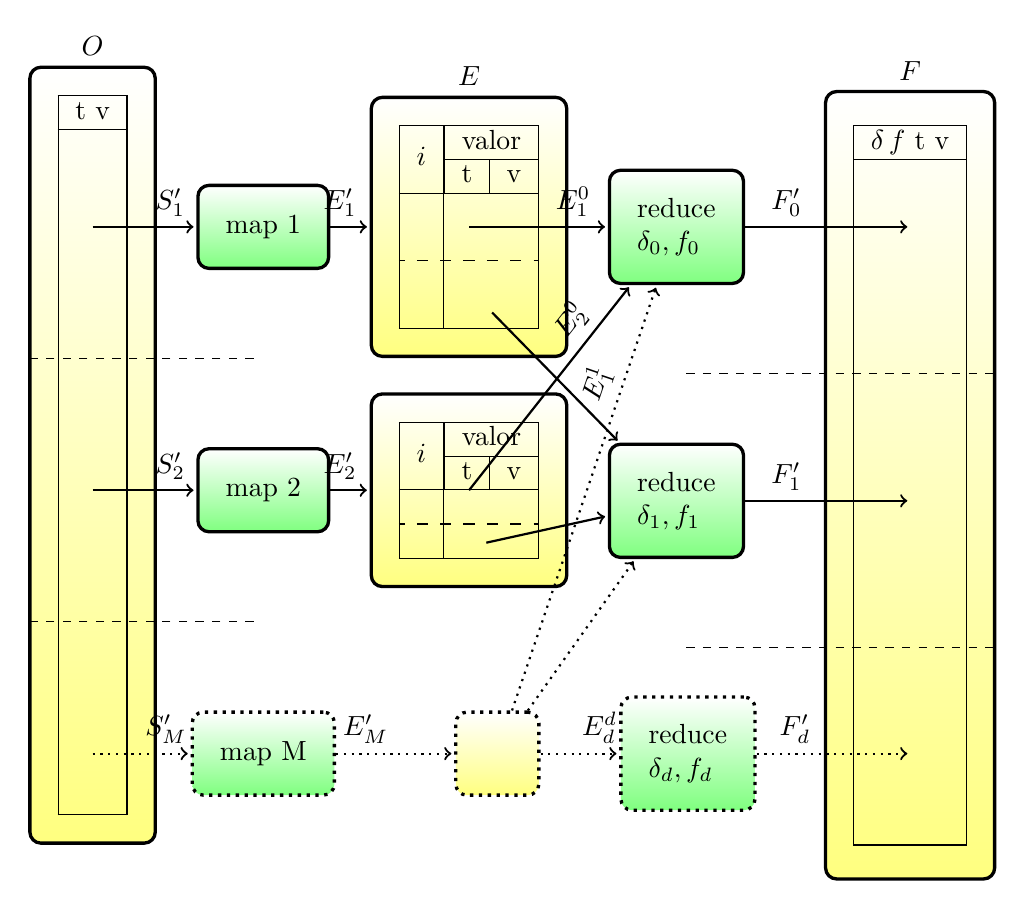
\begin{tikzpicture}

      \tikzset{
        mynode/.style={rectangle,rounded corners,draw=black, 
          very thick, inner sep=1em, minimum size=3em, text centered,
          groc},
        myarrow/.style={->, shorten >=1pt, thick},
        mylabel/.style={text width=7em, text centered},
        groc/.style={top color=white, bottom color=yellow!50},
        verd/.style={top color=white, bottom color=green!50},
        roig/.style={top color=white, bottom color=red!50},
      }  




 \node[mynode,verd] (m1) {map 1};
 \node (ml1) [below=of m1] {};
 \node[mynode,verd] (m2) [below=of ml1] {map 2};
 \node (ml2) [below=of m2] {};
 \node[mynode,verd,dotted] (mn) [below=of ml2] {map M};


 \node[mynode] (d1) [right=0.5cm of m1] {
   \begin{tabular}{|c|cc|}\hline
     \multirow{2}{*}{$i$} & \multicolumn{2}{|c|}{valor} \\\cline{2-3}
       & \multicolumn{1}{|c|}{t} & v \\\hline
      & & \\
      & &\\\hdashline
      & &\\
      & &\\\hline
   \end{tabular}
 };

 \node[mynode] (d2) [right=0.5cm of m2] {
   \begin{tabular}{|c|cc|}\hline
     \multirow{2}{*}{$i$} & \multicolumn{2}{|c|}{valor} \\\cline{2-3}
       & \multicolumn{1}{|c|}{t} & v \\\hline
      & &\\\hdashline
      & &\\\hline
   \end{tabular}
 };

 \node[mynode,dotted] (dn) [right=1.5cm of mn] {};



 \node[mynode,verd] (r1) [right=0.5cm of d1] {\parbox{1cm}{reduce $\delta_0,f_0$}};
 \node[mynode,verd] (r2) [below=2cm of r1] {\parbox{1cm}{reduce $\delta_1,f_1$}};
 \node[mynode,verd,dotted] (rn) [right=1cm of dn] {\parbox{1cm}{reduce $\delta_d,f_d$}};




 \node[mynode] (o) [above left=1.5cm and 0.5cm of m1, anchor=north east] {
   \begin{tabular}{|c|}\hline
     t v \\\hline
       \\
       \\
     \parbox[c][7cm][s]{0cm}{\vfill} \\
       \\
       \\\hline
   \end{tabular}
 };
 \node [above=0cm of o] {$O$};
 \node[mynode,minimum height=10cm] (f) [above right=of r1, anchor=north west] {
   \begin{tabular}{|c|}\hline
    $\delta\, f$ t v \\\hline
       \\
        \\
     \parbox[c][7cm][s]{0cm}{\vfill}  \\
        \\
        \\\hline
   \end{tabular}
};
 \node [above=0cm of f] {$F$};
 \node [above=0cm of d1] {$E$};




 \draw[dashed] (ml1) -- (ml1-|o.west);
 \draw[dashed] (ml2) -- (ml2-|o.west);

 \draw[myarrow] (o.center|-m1) -- (m1)  node[sloped,above,near end] {$S'_1$};
 \draw[myarrow] (o.center|-m2) -- (m2) node[sloped,above,near end] {$S'_2$};
 \draw[myarrow,dotted] (o.center|-mn) -- (mn) node[sloped,above,near end] {$S'_M$};


 \draw[myarrow] (m1) -- (d1) node[sloped,above,near start] {$E'_1$};
 \draw[myarrow] (m2) -- (d2) node[sloped,above,near start] {$E'_2$};
 \draw[myarrow,dotted] (mn) -- (dn)  node[sloped,above,near start] {$E'_M$};

 \draw[myarrow] (d1.center) -- (r1) node[sloped,above,near end] {$E_{1}^0$};
 \node (d1b) [above=3ex of d1.280] {}; 
 \draw[myarrow] (d1b.center) -- (r2) ;

 \draw[myarrow] (d2.center) -- (r1) node[sloped,above,near end] {$E_{2}^0$};
 \node (d2b) [above=3ex of d2.280] {}; 
 \draw[myarrow] (d2b.center) -- (r2) ;

 \draw[myarrow,dotted] (dn) -- (r1) node[sloped,above,near end] {$E_{1}^1$};
 \draw[myarrow,dotted] (dn) -- (r2);
 \draw[myarrow,dotted] (dn) -- (rn) node[sloped,above,near end] {$E_{d}^d$};


 \node (r1l) [below=of r1] {};
 \draw[dashed] (r1l) -- (r1l-|f.east);
 \node (r2l) [below=of r2] {};
 \draw[dashed] (r2l) -- (r2l-|f.east);


 \draw[myarrow] (r1) -- (r1-|f.center)  node[sloped,above,near start] {$F'_0$};
 \draw[myarrow] (r2) -- (r2-|f.center)  node[sloped,above,near start] {$F'_1$};
 \draw[myarrow,dotted] (rn) -- (rn-|f.center)  node[sloped,above,near start] {$F'_d$};


  \end{tikzpicture}
  
  \caption{Esquema de funcionament de RoundRobindoop}
  \label{fig:roundrobindoop:esquema}
\end{figure}






Les dades originals són la sèrie temporal $S$ és a dir un conjunt de
parelles de temps i valor, a les quals anomenem mesures. Un sèrie
temporal es pot partir en trossos on cada tros és un subconjunt de
mesures, és a dir una subsèrie temporal. Per tant, cada operació map
rep una subsèrie temporal de l'original: $S'_1 =
\{m_0,\dotsc,m_{o1}\}, S'_2 = \{m_{o1+1},\dotsc,m_{o2}\}, \dotsc, S'_M
= \{\dotsc,m_{k}\}$ on $M$ són el nombre de maps i $o_1,o_2\in
\glssymbol{not:N}$, $o_1 < o_2 < k$.



Les dades d'entremig són les sèries temporals dels buffers, és a dir
les mesures pendents de consolidar per a cada subsèrie resolució.
Així doncs, les dades d'entremig vistes com a conjunt són un conjunt
de dades pendents de consolidar $E=\{ D_{0}, \dotsc, D_t\}$ on cada
dada pendent de consolidar és un tuple $D=(i,m)$ on $i=(\delta,f,t_b)$
funciona com a identificador i $m=(t,v)$ com a valor.  És a dir, que
classifica cada mesura $m$ a quines resolucions s'han de consolidar
identificades pel pas de consolidació $\delta$, per la funció
d'agregació d'atributs $f$ i pel temps resultant de consolidació
$t_b$. Per tant, cada operació map resulta en un subconjunt de les
dades d'entremig: $E'_1=\{ (\delta_0,f_0, t_{b0}^0, t_0,v_0),
(\delta_1,f_1, t_{b1}^0, t_0,v_0), \dotsc , (\delta_d,f_d, t_{bd}^0,
t_0,v_0), (\delta_0,f_0, t_{b0}^1, t_1,v_1), \dotsc, (\delta_d,f_d,
t_{bd}^{o1}, t_{o1},v_{o1}) \}$, i $E'_2$ i $E'_M$ de manera similar.
En total, les dades d'entremig tenen un cardinal de $|E|=t+1=|e||S|$
és a dir la quantitat de resolucions de l'esquema multiplicat per la
quantitat de mesures de la sèrie temporal original.


Un cop calculades, les dades d'entremig $E$ s'ordenen i
s'agrupen per identificadors $(\delta,f, t_b)$ idèntics.  Així s'obté
unes dades d'entremig ordenades, de les quals expressem a continuació
cada subconjunt de forma simplificada agrupant per $\delta$ i $f$
sense tenir en comte els $t_b$. Siguin $ t_b, t,v$ variables lliures,
cada subconjunt agrupat de $E$ té la forma:
% Del subconjunt $E'_1$ s'obtenen els subconjunts $O_0^0= \{  (\delta_0,f_0, t_{b0}^0, t,v) \in E'_1 \}, O_0^1= \{  (\delta_0,f_0, t_{b0}^1, t,v) \in E'_1 \},\dotsc,  O_0^d= \{  (\delta_0,f_0, t_{b0}^{r0}, t,v) \in E'_1 \}$
a partir del subconjunt $E'_1$ s'obtenen $E_1^0=\{ (\delta_0,f_0, t_b,
t,v) \in E'_1 \}, E_1^1=\{ (\delta_1,f_1, t_b, t,v) \in E'_1 \},
\dotsc, E_1^d=\{ (\delta_d,f_d, t_b, t,v) \in E'_1 \}$, i de manera
similar s'obtenen els subconjunts agrupats a partir de
$E'_2,\dotsc,E'_d$.  D'aquesta manera cada operació reduce rep, en la
forma simplificada, tots els tuples de $E$ amb el mateix $\delta$ i
$f$: per a $\delta_0$ i $f_0$ rep $E^0 = E_1^0 \cup E_2^0 \cup \dotsb
\cup E_d^0$, per a $\delta_1$ i $f_1$ rep $E^1$, etc.  Com hem dit,
hem expressat aquests conjunts de forma simplificada per a $\delta$ i
$f$ tot i a més hi ha un reduce per a cada $t_b$ diferent; a
continuació per a les dades finals ho expressem de totes dues maneres.



Les dades finals són les sèries temporals dels discs, és a dir les
mesures consolidades per a cada subsèrie resolució. Així doncs, les
dades finals vistes com a conjunt són un conjunt de dades consolidades
$F=\{ D'_{0}, \dotsc, D'_r\}$ on cada dada consolidada és un tuple
$D'=(\delta,f,m')$ que indica quina mesura $m'=(t_b,v')$ és i a quin
disc pertany identificat per $\delta$ i $f$.  Per tant, cada operació
reduce calcula un subconjunt de $F$: $F_0^0
=\{(\delta_0,f_0,t_{b0}^0,v_0^0)\}, F_0^1
=\{(\delta_0,f_0,t_{b0}^1,v_0^1)\}, \dotsc, F_0^{r0}
=\{(\delta_0,f_0,t_{b0}^{r0},v_0^{r0})\}, F_1^0= \dotsc, F_1^{r1}=
\dotsc, F_d^0= \dotsc, F_d^{rd}=
\{(\delta_d,f_d,t_{bd}^{rd},v_d^{rd})\}$ on el nombre de mesures
consolidades per cada disc és afitat als cardinals màxims, $r_0 +1
\leq k_0, r_1 +1 \leq k_1, \dotsc r_d +1 \leq k_d$, i per tant el
nombre total de reduces està afitat a $|F| \leq k_0+k_1\dotsb+k_d$.
Per a simplificar la~\autoref{fig:roundrobindoop:esquema} s'han
agrupat els reduce per $\delta$ i $f$, és a dir $F'_0 =
\{(\delta_0,f_0,t_{b0}^0,v_0^0),(\delta_0,f_0,t_{b0}^1,v_0^1),\dotsc,
(\delta_0,f_0,t_{b0}^{r0},v_0^{r0})\}$, etc.\ i per tant $d+1= |e|$
són el nombre total de reduces agrupats.



L'operació map calcula les dades d'entremig a partir de les dades
originals i un esquema multiresolució, treballa en subconjunts de les
dades per a així poder-se computar para\l.lelament.
\begin{definition}[Operació Map]
  Sigui $S'=\{m_0,\dotsc,m_{o1}\}$ una subsèrie temporal de les dades
  originals, $e=\{ (\delta_0,f_0,\tau_0,k_0),\ldots,
  (\delta_d,f_d,\tau_d,k_d)\}$ un esquema de multiresolució i
  $E'=\{(\delta_0,f_0, t_{b0}^0, t_0,v_0),\dotsc, \dotsc,
  (\delta_d,f_d, t_{bd}^{o1}, t_{o1},v_{o1}) \}$ un subconjunt de les
  dades d'entremig abans de ser ordenades, l'operació map de
  l'algoritme MapReduce és $E'=\operatorname{map}(S',e)$ on $E'=
  \forall m \in S': \bigcup\operatorname{classifica}(m,e)$.

  La funció $\operatorname{classifica}$ indica per a cada mesura a quins
  discs s'ha de consolidar: $\operatorname{classifica}(m,e)=\{ \forall
  (\delta,f,\tau,k) \in e: (\delta,f,\tau+n\delta,t,v) |
  \tau+(n-1)\delta < t \leq \tau+n\delta, n\in\glssymbol{not:Z}, t >
  \tau \}$. Cal tenir en compte que $t > \tau$ indica que $\tau$ és el temps
  d'inici de la resolució i per tant no té sentit incloure mesures
  anteriors.
\end{definition}






Hi ha dues restriccions a la funció $\operatorname{classifica}$ que
hem definit: 
\begin{itemize}

\item S'assumeix que la $f$ treballa sobre l'interval de la sèrie
  original $S(\tau+(n-1)\delta ,\tau+n\delta]$. En cas que no sigui
  així per a la $f$ escollida, caldria modificar aquests intervals de
  classificació. A continuació d'aquest apartat contextualitzem aquest
  problema de les $f$.

\item No es tenen en compte els cardinals màxims. Si es volen tenir en
  compte, cal adequar bé els $\tau$ inicials. Així sigui $e$ l'esquema
  de multiresolució original, per a tenir en compte els cardinals
  màxims s'haurà d'usar un nou esquema $e'$ en què cada $\tau$
  original sigui canviat a un altre temps de consolidació múltiple
  $\tau'= \tau+n\delta$ (1) on $n\in\glssymbol{not:Z}$.  \emph{Càlcul
    de $n$:} es coneix $t_k=T(\max(S))$ i per a tenir en compte els
  cardinals s'ha de complir que $\tau'+k\delta \leq t_k$ (2), és a dir
  que les mesures entre $[\tau'+k\delta,t_k]$ encara no es poden
  consolidar.  Substituint la (1) a la (2) $\tau+n\delta+k\delta \leq
  t_k$, operant $\tau+(n+k)\delta \leq t_k$ i $n \leq
  \frac{t_k-\tau}{\delta}-k$ d'on es conclou que $n = \left\lfloor
    \frac{t_k-\tau}{\delta}-k \right\rfloor$ .  A més a més, si no es
  considera vàlid $\tau'<\tau$, és a dir que no es volen mesures abans
  del temps d'inici original, aleshores $n$ com a mínim pot valdre
  zero.

\end{itemize}



\begin{example}[Classificació d'una mesura en les resolucions]
  Sigui l'esquema de multiresolució
  $e=\{(\delta_0=2,f_0,\tau_0=0,k_0=4),(\delta_1=5,f_1,\tau_1=10,k_1=3)\}$
  i la mesura $m=(25,1)$, aquesta és classificada per a consolidar-se
  en les dues resolucions $\operatorname{classifica}(m,e)=\{
  (2,f_0,t_{b0},25,1), (5,f_1,t_{b1},25,1) \}$ on
  $\tau_0+(n-1)\delta_0 < 25 \leq \tau_0+n\delta_0,
  n\in\glssymbol{not:Z}$ i $t_{b0}=\tau_0+n\delta_0 = 26$, i de manera
  semblant $t_{b1}= 25$.

  Ara es volen tenir en compte els cardinals màxims, sigui
  $t_k=T(\max(S))=35$ el temps de la mesura màxima de la sèrie
  temporal original. Aleshores cal canviar l'esquema de multiresolució
  $e'=\{(\delta_0=2,f_0,\tau'_0,k_0=4),(\delta_1=5,f_1,\tau'_1,k_1=3)\}$
  on $\tau'_0=26$ i $\tau'_1=20$. La classificació esdevé
  $\operatorname{classifica}(m,e')=\{ (5,f_1,25,25,1) \}$ on no hi ha
  la resolució $\delta_0,f_0$ perquè $25< \tau'_0$.
\end{example}





Un cop s'han obtingut les dades d'entremig $E$, el sistema com per
exemple Hadoop agrupa els tuples de $E$ amb el mateix identificador i
els processa a un mateix reduce. És a dir, sigui $E$ la unió de tots
els $E'$ calculats pels map, un subconjunt de les dades ordenades és
$E''_{\delta,f,t_b} = \{ (\delta,f,t_b,m) \in E \}$.  L'operació
reduce calcula les dades finals a partir de les dades d'entremig
ordenades, treballa en subconjunts de les dades per a així poder-se
computar para\l.lelament.
\begin{definition}[Operació Reduce]
  Sigui $E''= \{ (\delta,f,t_b,m_0) ,\dotsc, (\delta,f,t_b,m_k) \}$ un
  subconjunt de les dades d'entremig ordenades i $F'=\{
  (\delta,f,t_b,v) \}$ un subconjunt de les dades finals, l'operació
  reduce de l'algoritme MapReduce és $F'=\operatorname{reduce}(E'')$
  on $F'= (\delta,f,t_b,v)$ i $v= V( f(\{m_0,\dotsc,m_k\},i))$ i
  $i=[t_b-\delta,t_b]$.
\end{definition}

L'expressió de l'interval $i$ es pot ometre ja que l'operació map ja
ha classificat les mesures d'aquest interval, tot i així l'indiquem
per a seguir la forma genèrica $f(S,i)$ de les funcions d'agregació
d'atributs de la definició. A continuació d'aquest apartat
contextualitzem aquest problema de les $f$.


En conclusió, el map i el reduce no es corresponen exactament
amb les definicions de les funcions de $\glssymbol{not:sgstm:dmap}$ i
$\glssymbol{not:sgstm:multiresolucio}$ \todo{ref a la secció?}, sinó
que el map classifica les mesures de la sèrie temporal segons el
buffer que els correspon i el reduce calcula les mesures consolidades
per un disc. És a dir, que un map i un reduce equivalen a la
funcionalitat de la funció $\glssymbol{not:sgstm:dmap}$ però el
conjunt de tots els maps i reduces equivalen a la funció de
$\glssymbol{not:sgstm:multiresolucio}$, sense expressar-ho en forma de
sèrie temporal total.



\subsubsection{Quant a les $f$ a RoundRobindoop}
\label{sec:mapreduce:f}

Al model de \gls{SGSTM} hem definit de forma genèrica les funcions
d'agregació d'atributs com a $m=f(S,i)$ (v. def.\todo{ref}). Aquestes funcions
principalment realitzen dues operacions: una selecció sobre la sèrie
temporal i una agregació de les mesures seleccionades. 

A RoundRobindoop, l'operació de selecció es duu a terme a l'etapa de
map i en canvi l'agregació, a l'etapa de reduce.  En l'algoritme de
MapReduce definit per a RoundRobindoop usem el model de $f$ descrit
anteriorment, però per a implementar correctament aquestes funcions
cal interpretar-ne el significat per a l'etapa de map i per a la de
reduce. És a dir, cada $f$ hauria de tenir dos components: un amb les
operacions de selecció per a ser usades en els map i l'altre amb les
operacions d'agregació per als reduce.


Així doncs, caldria afegir en els paràmetres de RoundRobindoop
l'operació de selecció d'interval per a cada $f$ que s'utilitzi. Però
això complica la resolució de l'algoritme de MapReduce. Per exemple,
resoldre l'interval temporal \gls{zohe}
--$S[t_0,t_f]^{\glssymbol{not:zohe}} = S(t_0,t_f] \cup \{
(t_f,V(\inf(S[t_f,+\infty))) \}$ (v.~def.\todo{ref a la def})--
implica conèixer la mesura següent a un $t_f$ i per tant treballar
sobre tota la sèrie temporal original, cosa que no és possible perquè
en les etapes map només es treballa sobre un subconjunt de la sèrie
temporal original. Això no obstant, per al RoundRobindoop definit, si
considerem que la sèrie temporal no té inframostreig aleshores en l'etapa
map podem fer la selecció prèvia per l'interval
$S(t_b-\delta,t_b+\delta]$, és a dir assumim que hi ha mesura a
$[t_b,t_b+\delta]$, i a l'etapa reduce ja es calcularà correctament
$f(S,[t_b-\delta,t_b])$. 


Recordem que en l'algoritme de RoundRobindoop definit hem assumit que
l'interval de selecció en l'etapa map sempre és $(t_b-\delta,t_b]$ i
en l'etapa reduce usem el model genèric d'agregació $f(S,i)$ tot i que
les mesures ja han estat seleccionades. Per tant, la interpretació en
l'etapa map no és vàlida per a totes les $f$.

Per tal d'ampliar l'etapa map, proposem una nova funció de
classificació que admeti ampliar l'interval de selecció. Si en la
classificació definida cada mesura es classificava en un i només un
$t_b$ per a cada resolució, en la nova funció de classificació es pot
escollir a quants $t_b$ es classifica cada mesura.  Sigui
$\operatorname{classifica}(m,e)$ la funció de classificació original i
sigui $l,g\in\glssymbol{not:N}$ les quantitats desitjades, la nova funció
de classificació és $\operatorname{classifica}'(m,e,l,g)=\{ \forall
(\delta,f,\tau,k) \in e: (\delta,f,\tau+(n-G_g)\delta,t,v), \dotsc,
(\delta,f,\tau+(n-G_0)\delta,t,v), (\delta,f,\tau+n\delta,t,v),
(\delta,f,\tau+(n+L_0)\delta,t,v), \dotsc,
(\delta,f,\tau+(n+L_l)\delta,t,v) | \tau+(n-1)\delta < t \leq
\tau+n\delta, n\in\glssymbol{not:Z}, t > \tau \}$ on
$L=\{1,2,\dotsc,l\}$ i $G=\{1,2,\dotsc,g\}$. El paràmetre $l$
permet classificar una mesura en temps posteriors i el paràmetre $g$
en temps anteriors; si ho observem des del punt de vista de la
selecció d'interval $S(t_b-(l+1)\delta,t_b+g\delta]$, el paràmetre $l$
permet estendre l'interval cap a l'esquerra i $g$ cap a la dreta.

\begin{example}[Classificació d'una mesura per \gls{zohe}]
  \label{ex:mapreduce:fzohe} 
  Com ja hem comentat, per a les funcions d'agregació d'atributs de la
  família \gls{zohe} s'ha d'aproximar l'interval temporal \gls{zohe} a
  una selecció en l'interval $S(t_b-\delta,t_b+\delta]$. És a dir, que
  la funció de classifica ha de retornar dues classificacions per a
  cada mesura, una amb $t_b$ i l'altra amb $t_b-\delta$. Per tant, per
  aquesta família $g=1$ i $l=0$.

  Sigui l'esquema de multiresolució
  $e=\{(\delta_0=2,f_0,\tau_0=0,k_0=4),(\delta_1=5,f_1,\tau_1=10,k_1=3)\}$
  i la mesura $m=(25,1)$, aquesta és classificada per a consolidar-se
  en les dues resolucions i en els dos instants per a cada un:
  $\operatorname{classifica}'(m,e,l=0,g=1)=\{
  (2,f_0,t_{b0}-g\delta_0,25,1), (2,f_0,t_{b0},25,1),
  (5,f_1,t_{b1}-g\delta_1,25,1), (5,f_1,t_{b1},25,1) \}$ on $t_{b0}=
  26$, $t_{b0}-g\delta_0= 24$, $t_{b1}= 25$ i $t_{b1}-g\delta_1= 20$.
  És a dir, es pot interpretar per a $\delta_0$ que quan es consolidi
  l'instant $24$ s'ha de fer la selecció $S(22,26]$ i per l'instant
  $26$ s'ha de fer la selecció $S(24,28]$, intervals en els quals hi
  ha la mesura $(25,1)$.

  A continuació, en l'apartat d'execució de l'algoritme, utilitzarem un exemple
  amb aquests processos de classificació.
\end{example}






En resum, el model de programació MapReduce limita les capacitats dels
\gls{SGSTM}, sobretot pel que fa a les funcions d'agregació
d'atributs. 






\subsection{Execució de l'algoritme}

\lstMakeShortInline[style=sh]{@}

Hadoop s'encarrega de l'execució de l'algoritme de MapReduce i de la
gestió de les dades d'entrada i de sortida.  Per a implementar-lo, cal
dissenyar un programa per al map i un programa per al reduce, els
quals reben de Hadoop els subconjunts de dades escaients i han de
retornar els subconjunts també escaients.  

Es pot utilitzar diferents llenguatges de programació a l'hora
d'implementar l'algoritme de MapReduce, hem escollit el llenguatge
Python \parencite{python:doc2}.  Implementem l'algoritme de MapReduce
que hem definit, RoundRobindoop, en un mateix programa que anomenem
@rrdoop.py@. El programa té un paràmetre que permet escollir l'etapa,
@rrdoop.py -map@ o @rrdoop.py -reduce@. A més també hi ha un paràmetre
per a definir l'esquema de multiresolució utilitzat, %
@rrdoop.py -map -schema e@.

El programa es comunica amb Hadoop mitjançant l'entrada estàndard
(stdin) per a rebre dades i mitjançant la sortida estàndard (stdout)
per a retornar els resultats.  Gràcies a la generalització del
programa amb comunicació per stdin i stdout, també es pot executar
l'algoritme de MapReduce al shell del sistema operatiu, cosa que
facilita l'experimentació amb l'algoritme.  Així, a continuació,
primer mostrem l'execució pas a pas de @rrdoop.py@ al shell i després
mostrem l'execució a Hadoop.



\subsubsection{Execució a la shell}

El~\autoref{lst:rrdoop:shell} és l'execució de
@rrdoop.py@ al shell del sistema operatiu. Només hi ha un procés map i
un procés reduce. Es comuniquen les dades a través de pipes (@|@) de la
shell i d'un procés d'ordenació (@sort@) que emula el procés
d'ordenació per identificador que faria Hadoop. A més, també s'emula
el procés de lectura (@cat@) de les dades originals.

\begin{lstlisting}[style=sh,caption=Execució a la shell de
  rrdoop.py,label=lst:rrdoop:shell]
cat original.csv | rrdoop.py -map -schema e.pickle -mapg 1 | sort -k1,1 | rrdoop.py -reduce -schema e.pickle  > final.csv
\end{lstlisting}


Les dades d'entrada són un fitxer, que també podrien ser fitxers de
dades, de les quals Hadoop en processa conjunts de línies a cada
procés map. Aquestes dades no cal que siguin ordenades i cal tenir en
compte que es poden trencar per qualsevol línia, tot i que Hadoop
permet configurar etapes que defineixin com s'han de partir els
fitxers.  Al~\autoref{lst:rrdoop:stdin} mostrem les dades d'entrada
emmagatzemades en el fitxer @original.csv@, que es corresponen
amb la sèrie temporal ja utilitzada
al~\autoref{lst:roundrobinson:ex1}.  Aquest fitxer de dades té format
de \gls{CSV}, com ja s'ha vist al~\autoref{lst:pytsms:storage} en les
funcionalitats complementàries per a l'emmagatzematge de Pytsms.
\begin{lstlisting}[style=file,caption=Dades d'entrada original.csv,label=lst:rrdoop:stdin]
1,6
8,5
5,2
10,0
14,1
19,6
26,6
29,0
22,11
\end{lstlisting}


El fitxer @original.csv@ es transmet a través de @cat@ i pipe a
l'stdin del procés de map %
@rrdoop.py -map -schema e.pickle -mapg 1@.  El procés de map té un esquema de
multiresolució com a paràmetre, @rrdoop.py@ a través del paràmetre
@-schema@ admet una sèrie temporal multiresolució en format Pickle,
com s'ha vist al~\autoref{lst:roundrobinson:storage}, l'esquema de la
qual serà el que s'utilitzi. En aquest cas, @e.pickle@ es correspon
amb el fitxer @mrd.pickle@ del~\autoref{lst:roundrobinson:storage} i
per tant amb l'esquema de multiresolució
del~\autoref{lst:roundrobinson:ex1}:
$e=\{(\delta_0=5,k_0=4,f_0=\glssymbol{not:sgstm:meanzohe},\tau_0=0),(\delta_1=10,k_1=2,f_1=\glssymbol{not:sgstm:maxzohe},\tau_1=0)\}$.


En aquest exemple d'esquema de multiresolució s'usen funcions
d'agregació d'atributs de la família \gls{zohe}. Com ja hem comentat a
l'\autoref{ex:mapreduce:fzohe}, s'ha de canviar la selecció que
l'etapa map duu a terme. A tal efecte RoundRobindoop admet un
paràmetre @-mapg@ per a indicar l'expansió de la classificació cap a
la dreta. Aproximem l'interval temporal \gls{zohe} a una selecció en
l'interval $(t_b-\delta,t_b+\delta]$, és a dir que hem d'expandir un
interval @-mapg 1@.  RoundRobindoop també admet un paràmetre @-mapl@
per a l'expansió cap a l'esquerra.


El procés de map retorna el resulta a través de l'stdout, el qual es
mostra al~\autoref{lst:rrdoop:sortidamap} i es correspon amb les dades
d'entremig de MapReduce. El format és el requerit per Hadoop, és a dir
cada línia és una parella d'identificador i valor separats per un
tabulador. L'identificador és $(\delta,\tau,t_b)$ però escrit en el
format $\delta$/$\tau$--$t_b$ i el valor és $(t,v)$ escrit separat per
un espai. Es pot observar com es comença classificant la primera
mesura $(1,6)$ en l'instant de consolidació $t_b=10$ per $\delta_1$ i
$t_b=5$ per $\delta_0$.  A continuació la mesura $(8,5)$ es classifica
a l'instant de consolidació $t_b=10$ per $\delta_1$ i en els $t_b=10$
i $t_b=5$ per $\delta_0$, en aquest darrer cas s'aplica l'aproximació
de la selecció \gls{zohe} per l'interval $(t_b-\delta,t_b+\delta]$;
cal destacar que en els casos anteriors no s'aplica perquè resultaria en
un $t_b<= \tau$.  I així per a totes fins a la darrera mesura
$(22,11)$.
\begin{lstlisting}[style=stdout,caption=Sortida del procés map,label=lst:rrdoop:sortidamap]
10/maximum_zohe-10	1 6.0
5/mean_zohe-5	1 6.0
10/maximum_zohe-10	8 5.0
5/mean_zohe-10	8 5.0
5/mean_zohe-5	8 5.0
10/maximum_zohe-10	5 2.0
5/mean_zohe-5	5 2.0
10/maximum_zohe-10	10 0.0
5/mean_zohe-10	10 0.0
5/mean_zohe-5	10 0.0
10/maximum_zohe-20	14 1.0
10/maximum_zohe-10	14 1.0
5/mean_zohe-15	14 1.0
5/mean_zohe-10	14 1.0
10/maximum_zohe-20	19 6.0
10/maximum_zohe-10	19 6.0
5/mean_zohe-20	19 6.0
5/mean_zohe-15	19 6.0
10/maximum_zohe-30	26 6.0
10/maximum_zohe-20	26 6.0
5/mean_zohe-30	26 6.0
5/mean_zohe-25	26 6.0
10/maximum_zohe-30	29 0.0
10/maximum_zohe-20	29 0.0
5/mean_zohe-30	29 0.0
5/mean_zohe-25	29 0.0
10/maximum_zohe-30	22 11.0
10/maximum_zohe-20	22 11.0
5/mean_zohe-25	22 11.0
5/mean_zohe-20	22 11.0
\end{lstlisting}


A continuació el procés d'ordenació @sort -k1,1@ ordena per
identificadors, el qual es mostra
al~\autoref{lst:rrdoop:sortidasort}. Hadoop agruparia els mateixos
identificadors i els transmetria a l'stdin d'un procés de reduce.
Observem per exemple la primera resolució @10/maximum_zohe-10@ que
conté les mesures en els instants de temps 10, 14, 1 ,19, 5 i 8;
l'agregació posterior haurà de treballar en l'interval \gls{zohe}
[0,10] i per tant ara queda clar que les mesures de 14 i 19 no són
necessàries, però això no ho podíem resoldre en l'etapa de map.
\begin{lstlisting}[style=stdout,caption=Sortida del procés d'ordenació,label=lst:rrdoop:sortidasort]
10/maximum_zohe-10	10 0.0
10/maximum_zohe-10	14 1.0
10/maximum_zohe-10	1 6.0
10/maximum_zohe-10	19 6.0
10/maximum_zohe-10	5 2.0
10/maximum_zohe-10	8 5.0
10/maximum_zohe-20	14 1.0
10/maximum_zohe-20	19 6.0
10/maximum_zohe-20	22 11.0
10/maximum_zohe-20	26 6.0
10/maximum_zohe-20	29 0.0
10/maximum_zohe-30	22 11.0
10/maximum_zohe-30	26 6.0
10/maximum_zohe-30	29 0.0
5/mean_zohe-10	10 0.0
5/mean_zohe-10	14 1.0
5/mean_zohe-10	8 5.0
5/mean_zohe-15	14 1.0
5/mean_zohe-15	19 6.0
5/mean_zohe-20	19 6.0
5/mean_zohe-20	22 11.0
5/mean_zohe-25	22 11.0
5/mean_zohe-25	26 6.0
5/mean_zohe-25	29 0.0
5/mean_zohe-30	26 6.0
5/mean_zohe-30	29 0.0
5/mean_zohe-5	10 0.0
5/mean_zohe-5	1 6.0
5/mean_zohe-5	5 2.0
5/mean_zohe-5	8 5.0
\end{lstlisting}


Finalment, el procés de reduce %
@rrdoop.py -reduce -schema e.pickle > final.csv@ obté de l'stdin les
dades del~\autoref{lst:rrdoop:sortidasort} i retorna les dades finals
per l'stdout que està redirigit al fitxer @final.csv@, el contingut
del qual es mostra al~\autoref{lst:rrdoop:sortidashell}.  Hadoop
emmagatzemaria aquestes dades en un fitxer o fitxers de dades.
Aquestes dades tenen el format $\delta$/$f$ $t_b$ $v$ on $(t_b,v)$ és
la mesura consolidada per a la resolució identificada per
$(\delta,f)$.

\begin{lstlisting}[style=file,caption=Dades de sortida final.csv,label=lst:rrdoop:sortidashell]
10/maximum_zohe	10 6.0
10/maximum_zohe	20 11.0
10/maximum_zohe	30 None
5/mean_zohe	10 3.0
5/mean_zohe	15 2.0
5/mean_zohe	20 7.0
5/mean_zohe	25 8.0
5/mean_zohe	30 None
5/mean_zohe	5 2.8
\end{lstlisting}

Així aquest resultat és el mateix que el de les consultes $\glssymbol{not:sgstm:seriedisc}(M,5,\glssymbol{not:sgstm:meanzohe})$ i $\glssymbol{not:sgstm:seriedisc}(M,10,\glssymbol{not:sgstm:maxzohe})$ del~\autoref{lst:roundrobinson:ex1} però amb les particularitats següents:

\begin{itemize}
\item RoundRobindoop no té en compte els cardinals màxims $k$ de les resolucions. Hi ha la mesura consolidada a l'instant $t_b=5$ per a la resolució $\delta_0=5$ que ja hauria d'haver estat eliminada per complir amb $k_0=4$.

\item RoundRobindoop no té en compte el temps màxim de la sèrie
  temporal original per a conèixer les mesures que encara no són
  consolidables. Hi ha la mesures en l'instant $t_b=30$ per a
  $\delta_0=5$ i $\delta_1=10$ que encara no podien ser calculades
  perquè $T(\max(S))=29$, de fet tenen valor nul (\emph{None}) a causa
  que l'interval \gls{zohe} no es pot calcular.

\item Així doncs, hi ha 9 mesures consolidades finals però 3 s'han de
  descartar. Per tant, per a la resolució $\delta_0=5$ hi ha 4 mesures
  i es compleix $4 \leq k_0=4$, i per a la resolució $\delta_1=10$ hi ha 2
  mesures i es compleix $2 \leq k_1=3$.
\end{itemize}




\subsubsection{Execució a Hadoop}


El~\autoref{lst:rrdoop:hadoop} mostra els passos d'execució de
@rrdoop.py@ a Hadoop. Primer cal copiar la sèrie temporal original a
\gls{HDFS}, després s'executa l'algoritme MapReduce i finalment es
recupera el resultat de \gls{HDFS}.  Hadoop streaming és l'eina que
permet l'execució a Hadoop de qualsevol programa, en qualsevol
llenguatge, que tingui el model de MapReduce.
Per a més detall sobre les ordres
i els processos vegeu la documentació de Hadoop~\parencite{hadoop}.
%http://hadoop.apache.org/docs/current/hadoop-mapreduce-client/hadoop-mapreduce-client-core/HadoopStreaming.html

\todo{simplificar alguns path, no cal tant detall aquí}

\begin{lstlisting}[style=sh,caption=Execució a Hadoop de
  rrdoop.py,label=lst:rrdoop:hadoop]
hadoop dfs -copyFromLocal original.csv /user/aleix/original.csv

hadoop jar /usr/lib/hadoop/contrib/streaming/hadoop-streaming*.jar -file rrdoop.py -file e.pickle  -mapper 'rrdoop.py -map -schema e.pickle -mapg 1' -reducer 'rrdoop.py -reduce -schema e.pickle' -input /user/aleix/original.csv -output /user/aleix/final

hadoop dfs -copyToLocal /user/aleix/final/part-00000 final.csv
\end{lstlisting}
%per esborrar: hadoop dfs -rmr /user/aleix/final
%requisit, tenir disponible roundrobinson, p.ex. cp -r ~/pfc_svn/src/roundrobinson/trunk/ /usr/local/lib/python2.7/dist-packages/roundrobinson

Per tal d'observar de manera senzilla l'execució de l'algoritme a
Hadoop hem realitzat una configuració anomenada \emph{Single Node
  Setup}, és a dir on només hi ha un computador que processa.  Un cop
verificat es podria estendre a una configuració de \emph{Cluster
  Setup}, en què hi hagués més computadors on distribuir les dades i
els processos.


El resultat és el mateix fitxer @final.csv@ que per a l'execució a la
shell, és a dir el~\autoref{lst:rrdoop:sortidashell}.  Hadoop gestiona
automàticament la distribució i la quantitat dels processos map i
reduce. Així, alguns dels map o reduces es poden ajuntar en el mateix
procés, per exemple els reduce poden rebre tant els subconjunts $E^0$
o $E''$ de la secció anterior, però mai se separa el mateix
identificador en diferents reduces. De fet, aquest és el cas quan
s'executa a la shell, on només hi ha un procés map i un de reduce.







% \subsubsection{Anàlisi de temps}


%Estaria bé comparar també amb pytsms, encara que s'ha de dir que no tenen res a veure perquè a pytsms no hem tingut gens en compte l'eficiència en el temps

% Per al temps s'hauria d'executar com a mínim 10 vegades cada experiment


% Analitzem el temps que triga en executar-se l'algoritme de MapReduce,
% tant en la shell com a Hadoop. En aquest darrer cas no incloem el
% temps de treballar amb el \gls{HDFS}.


% \begin{verbatim}
% * shell

% time cat matriu0.csv | ./rrdoop.py -map | sort -k1,1 | ./rrdoop.py -reduce > provant.csv::

%  real   0m21.639s
%  user   0m21.513s
%  sys    0m0.864s


% * hadoop

% time hadoop jar /usr/lib/hadoop/contrib/streaming/hadoop-streaming*.jar -file rrdoop.py -mapper 'rrdoop.py -map' -reducer 'rrdoop.py -reduce' -input /user/aleix/matriu0.csv -output /user/aleix/matriu::

%  real   0m28.314s
%  user   0m1.640s
%  sys    0m0.152s
% \end{verbatim}











\lstDeleteShortInline{@}



%%% Local Variables:
%%% TeX-master: "main"
%%% End:

  \caption{Esquema de funcionament de MapReduce}
  \label{fig:mapreduce:esquema}
\end{figure}



\begin{enumerate}

\item Hi ha unes dades originals que es poden partir en
  trossos. Hadoop està orientat a fitxers, mitjançant \gls{HDFS}, i
  per tant cada tros de dades és cadascun dels fitxers que es volen
  processar o bé conjunts de línies d'un fitxer.

\item Cada tros de les dades es processa mitjançant una operació
  map. Cada map es pot computar en para\l.lel i distribuït.

\item Cada operació map ha de retornar un nou conjunt de dades
  formats per parelles d'identificador i valor. Aquests conjunts de
  dades s'ordenen per identificador. 

\item Cada conjunt de dades amb el mateix identificador es processa
  mitjançant una operació reduce. Cada reduce es pot computar en
  para\l.lel i distribuït.

\item Cada reduce ha de retornar un tros del resultat final. És a dir,
  que unint les dades que retornen els reduce s'obtenen les dades
  finals. En l'orientació a fitxers de Hadoop, el resultat final és un
  fitxer, o bé un tros d'un fitxer, per a cada reduce.

\end{enumerate}



Per a resoldre un algoritme amb MapReduce, cal definir l'operació de
map i l'operació de reduce. El map ha de calcular un filtre sobre les
dades, sobretot establir grups de dades, i el reduce ha de calcular
agregacions o resums per a cada grup. MapReduce té una gran similitud
amb l'operació \emph{summarize} dels
\gls{SGBDR} \parencite[cap.~7]{date04:introduction8}, però separada
convenientment en les dues etapes.  A més, MapReduce imposa les
següents restriccions: les dades s'han de poder partir i l'algoritme
s'ha de poder expressar separat en les dues operacions de map i de
reduce.  \textcite{deanghemawat04:mapreduce} mostren exemples
d'algoritmes que es poden expressar amb MapReduce.



Un cop s'ha modelat un algoritme amb MapReduce, aleshores Hadoop ja és
capaç d'executar els maps i els reduces en para\l.lel i distribuïts. A
més, Hadoop també gestiona el compromís dels recursos entre el temps
de distribuir les dades, la quantitat de processos en para\l.lel que
s'han de crear i el temps afegit que suposa cada procés nou.








\section{RoundRobindoop}


RoundRobindoop implementa un \gls{SGSTM} específic que resol la funció
de multiresolució amb el model de programació MapReduce.  Per a
construir RoundRobindoop, primer dissenyem l'algoritme de MapReduce
que s'adequa a la multiresolució. Segon, proposem dues maneres per a
executar RoundRobindoop: amb Hadoop i la shell del sistema.



\subsection{Multiresolució amb MapReduce}

L'algoritme que implementem amb MapReduce és el de la funció de
multiresolució definida a la secció \todo{ref sec: multiresolucio: funcio}. Aquesta funció principalment té dues
parts, una de mapa i una de plec, que com ja s'ha dit no es poden
correspondre exactament amb les operacions de map i de reduce. 
 Així
doncs, dissenyem les operacions de map i de reduce que tenen el mateix
efecte que calcular la funció de multiresolució, en què el resultat
final no és la sèrie temporal total sinó el resultat de totes les
funcions $\glssymbol{not:sgstm:dmap}$, és a dir el resultat final són
les sèries temporals dels discs del model de \gls{SGSTM} la
concatenació dels quals resulta en la sèrie temporal total.



Sigui $S=\{m_0,m_1,\dotsc,m_k\}$ una sèrie temporal, i $e = \{
(\delta_0,f_0,\tau_0,k_0),\ldots, (\delta_d,f_d,\tau_d,k_d)\}$ els
paràmetres d'un esquema de multiresolució, definim l'algoritme
MapReduce que calcula $\operatorname{mapreduce}(S,e) = \{
(\delta_0,f_0,
\glssymbol{not:sgstm:dmap}(S,\delta_0,f_0,\tau_0,k_0)),\dotsc,
(\delta_c,f_c,\glssymbol{not:sgstm:dmap}(S,\delta_c,f_c,\tau_c,k_c))
\}$. És a dir, calcula tots els $\glssymbol{not:sgstm:dmap}$ possibles
i els identifica amb el pas de consolidació $\delta$ i la funció
d'agregació d'atributs $f$, els quals identifiquen les subsèries
resolució assumint que no n'hi ha de repetits.
%i que per tant tenenassociats el cardinal màxim $k$ i un instant de consolidació $\tau$.





L'esquema de funcionament de RoundRobindoop és el de
la~\autoref{fig:roundrobindoop:esquema}, el qual és la implementació
particular de l'esquema de la~\autoref{fig:mapreduce:esquema} per a la
multiresolució.  De forma resumida, RoundRobindoop en l'etapa de map
classifica les mesures en funció de a quin disc i temps resultant es
consolidaran i en l'etapa de reduce calcula la funció d'agregació per
a les mesures que s'hagin de consolidar al mateix disc.  A continuació
expliquem detalladament com són les dades originals ($O$), les
d'entremig ($E$) i les finals ($F$), i finalment definim l'operació de
map i la de reduce.





\begin{figure}[tp]
  \centering

  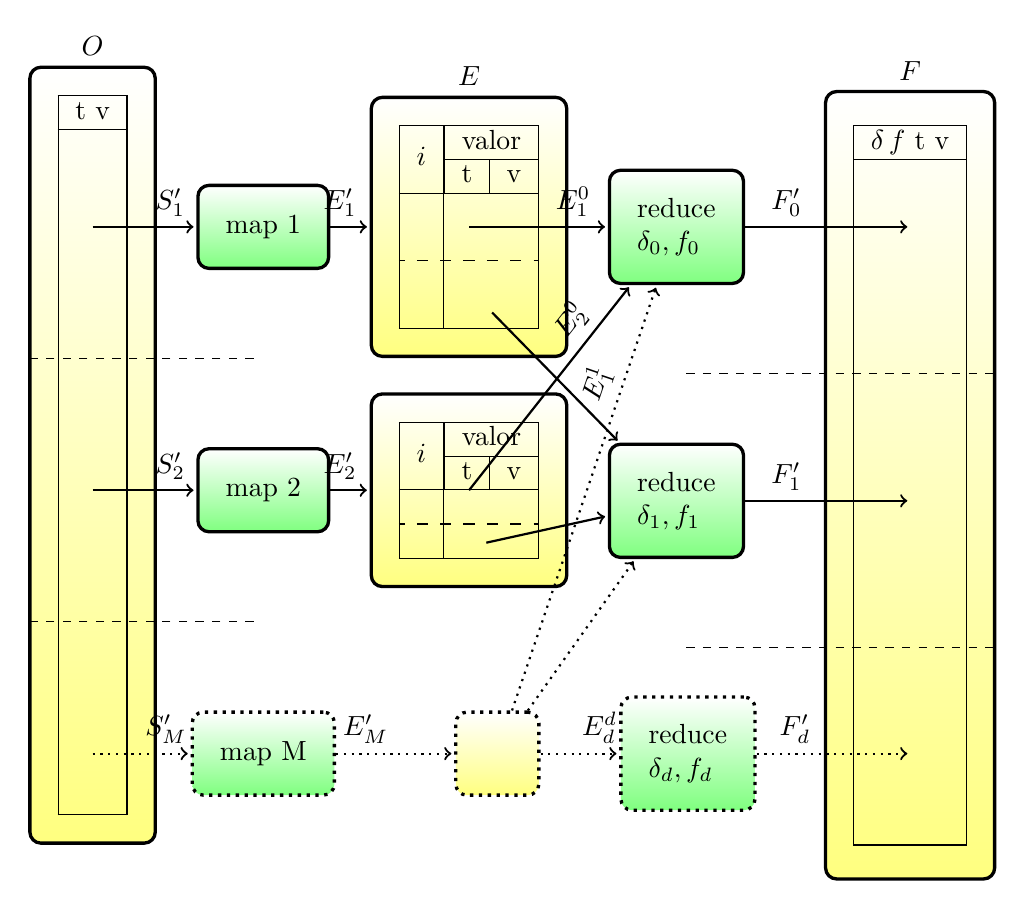
\begin{tikzpicture}

      \tikzset{
        mynode/.style={rectangle,rounded corners,draw=black, 
          very thick, inner sep=1em, minimum size=3em, text centered,
          groc},
        myarrow/.style={->, shorten >=1pt, thick},
        mylabel/.style={text width=7em, text centered},
        groc/.style={top color=white, bottom color=yellow!50},
        verd/.style={top color=white, bottom color=green!50},
        roig/.style={top color=white, bottom color=red!50},
      }  




 \node[mynode,verd] (m1) {map 1};
 \node (ml1) [below=of m1] {};
 \node[mynode,verd] (m2) [below=of ml1] {map 2};
 \node (ml2) [below=of m2] {};
 \node[mynode,verd,dotted] (mn) [below=of ml2] {map M};


 \node[mynode] (d1) [right=0.5cm of m1] {
   \begin{tabular}{|c|cc|}\hline
     \multirow{2}{*}{$i$} & \multicolumn{2}{|c|}{valor} \\\cline{2-3}
       & \multicolumn{1}{|c|}{t} & v \\\hline
      & & \\
      & &\\\hdashline
      & &\\
      & &\\\hline
   \end{tabular}
 };

 \node[mynode] (d2) [right=0.5cm of m2] {
   \begin{tabular}{|c|cc|}\hline
     \multirow{2}{*}{$i$} & \multicolumn{2}{|c|}{valor} \\\cline{2-3}
       & \multicolumn{1}{|c|}{t} & v \\\hline
      & &\\\hdashline
      & &\\\hline
   \end{tabular}
 };

 \node[mynode,dotted] (dn) [right=1.5cm of mn] {};



 \node[mynode,verd] (r1) [right=0.5cm of d1] {\parbox{1cm}{reduce $\delta_0,f_0$}};
 \node[mynode,verd] (r2) [below=2cm of r1] {\parbox{1cm}{reduce $\delta_1,f_1$}};
 \node[mynode,verd,dotted] (rn) [right=1cm of dn] {\parbox{1cm}{reduce $\delta_d,f_d$}};




 \node[mynode] (o) [above left=1.5cm and 0.5cm of m1, anchor=north east] {
   \begin{tabular}{|c|}\hline
     t v \\\hline
       \\
       \\
     \parbox[c][7cm][s]{0cm}{\vfill} \\
       \\
       \\\hline
   \end{tabular}
 };
 \node [above=0cm of o] {$O$};
 \node[mynode,minimum height=10cm] (f) [above right=of r1, anchor=north west] {
   \begin{tabular}{|c|}\hline
    $\delta\, f$ t v \\\hline
       \\
        \\
     \parbox[c][7cm][s]{0cm}{\vfill}  \\
        \\
        \\\hline
   \end{tabular}
};
 \node [above=0cm of f] {$F$};
 \node [above=0cm of d1] {$E$};




 \draw[dashed] (ml1) -- (ml1-|o.west);
 \draw[dashed] (ml2) -- (ml2-|o.west);

 \draw[myarrow] (o.center|-m1) -- (m1)  node[sloped,above,near end] {$S'_1$};
 \draw[myarrow] (o.center|-m2) -- (m2) node[sloped,above,near end] {$S'_2$};
 \draw[myarrow,dotted] (o.center|-mn) -- (mn) node[sloped,above,near end] {$S'_M$};


 \draw[myarrow] (m1) -- (d1) node[sloped,above,near start] {$E'_1$};
 \draw[myarrow] (m2) -- (d2) node[sloped,above,near start] {$E'_2$};
 \draw[myarrow,dotted] (mn) -- (dn)  node[sloped,above,near start] {$E'_M$};

 \draw[myarrow] (d1.center) -- (r1) node[sloped,above,near end] {$E_{1}^0$};
 \node (d1b) [above=3ex of d1.280] {}; 
 \draw[myarrow] (d1b.center) -- (r2) ;

 \draw[myarrow] (d2.center) -- (r1) node[sloped,above,near end] {$E_{2}^0$};
 \node (d2b) [above=3ex of d2.280] {}; 
 \draw[myarrow] (d2b.center) -- (r2) ;

 \draw[myarrow,dotted] (dn) -- (r1) node[sloped,above,near end] {$E_{1}^1$};
 \draw[myarrow,dotted] (dn) -- (r2);
 \draw[myarrow,dotted] (dn) -- (rn) node[sloped,above,near end] {$E_{d}^d$};


 \node (r1l) [below=of r1] {};
 \draw[dashed] (r1l) -- (r1l-|f.east);
 \node (r2l) [below=of r2] {};
 \draw[dashed] (r2l) -- (r2l-|f.east);


 \draw[myarrow] (r1) -- (r1-|f.center)  node[sloped,above,near start] {$F'_0$};
 \draw[myarrow] (r2) -- (r2-|f.center)  node[sloped,above,near start] {$F'_1$};
 \draw[myarrow,dotted] (rn) -- (rn-|f.center)  node[sloped,above,near start] {$F'_d$};


  \end{tikzpicture}
  
  \caption{Esquema de funcionament de RoundRobindoop}
  \label{fig:roundrobindoop:esquema}
\end{figure}






Les dades originals són la sèrie temporal $S$ és a dir un conjunt de
parelles de temps i valor, a les quals anomenem mesures. Un sèrie
temporal es pot partir en trossos on cada tros és un subconjunt de
mesures, és a dir una subsèrie temporal. Per tant, cada operació map
rep una subsèrie temporal de l'original: $S'_1 =
\{m_0,\dotsc,m_{o1}\}, S'_2 = \{m_{o1+1},\dotsc,m_{o2}\}, \dotsc, S'_M
= \{\dotsc,m_{k}\}$ on $M$ són el nombre de maps i $o_1,o_2\in
\glssymbol{not:N}$, $o_1 < o_2 < k$.



Les dades d'entremig són les sèries temporals dels buffers, és a dir
les mesures pendents de consolidar per a cada subsèrie resolució.
Així doncs, les dades d'entremig vistes com a conjunt són un conjunt
de dades pendents de consolidar $E=\{ D_{0}, \dotsc, D_t\}$ on cada
dada pendent de consolidar és un tuple $D=(i,m)$ on $i=(\delta,f,t_b)$
funciona com a identificador i $m=(t,v)$ com a valor.  És a dir, que
classifica cada mesura $m$ a quines resolucions s'han de consolidar
identificades pel pas de consolidació $\delta$, per la funció
d'agregació d'atributs $f$ i pel temps resultant de consolidació
$t_b$. Per tant, cada operació map resulta en un subconjunt de les
dades d'entremig: $E'_1=\{ (\delta_0,f_0, t_{b0}^0, t_0,v_0),
(\delta_1,f_1, t_{b1}^0, t_0,v_0), \dotsc , (\delta_d,f_d, t_{bd}^0,
t_0,v_0), (\delta_0,f_0, t_{b0}^1, t_1,v_1), \dotsc, (\delta_d,f_d,
t_{bd}^{o1}, t_{o1},v_{o1}) \}$, i $E'_2$ i $E'_M$ de manera similar.
En total, les dades d'entremig tenen un cardinal de $|E|=t+1=|e||S|$
és a dir la quantitat de resolucions de l'esquema multiplicat per la
quantitat de mesures de la sèrie temporal original.


Un cop calculades, les dades d'entremig $E$ s'ordenen i
s'agrupen per identificadors $(\delta,f, t_b)$ idèntics.  Així s'obté
unes dades d'entremig ordenades, de les quals expressem a continuació
cada subconjunt de forma simplificada agrupant per $\delta$ i $f$
sense tenir en comte els $t_b$. Siguin $ t_b, t,v$ variables lliures,
cada subconjunt agrupat de $E$ té la forma:
% Del subconjunt $E'_1$ s'obtenen els subconjunts $O_0^0= \{  (\delta_0,f_0, t_{b0}^0, t,v) \in E'_1 \}, O_0^1= \{  (\delta_0,f_0, t_{b0}^1, t,v) \in E'_1 \},\dotsc,  O_0^d= \{  (\delta_0,f_0, t_{b0}^{r0}, t,v) \in E'_1 \}$
a partir del subconjunt $E'_1$ s'obtenen $E_1^0=\{ (\delta_0,f_0, t_b,
t,v) \in E'_1 \}, E_1^1=\{ (\delta_1,f_1, t_b, t,v) \in E'_1 \},
\dotsc, E_1^d=\{ (\delta_d,f_d, t_b, t,v) \in E'_1 \}$, i de manera
similar s'obtenen els subconjunts agrupats a partir de
$E'_2,\dotsc,E'_d$.  D'aquesta manera cada operació reduce rep, en la
forma simplificada, tots els tuples de $E$ amb el mateix $\delta$ i
$f$: per a $\delta_0$ i $f_0$ rep $E^0 = E_1^0 \cup E_2^0 \cup \dotsb
\cup E_d^0$, per a $\delta_1$ i $f_1$ rep $E^1$, etc.  Com hem dit,
hem expressat aquests conjunts de forma simplificada per a $\delta$ i
$f$ tot i a més hi ha un reduce per a cada $t_b$ diferent; a
continuació per a les dades finals ho expressem de totes dues maneres.



Les dades finals són les sèries temporals dels discs, és a dir les
mesures consolidades per a cada subsèrie resolució. Així doncs, les
dades finals vistes com a conjunt són un conjunt de dades consolidades
$F=\{ D'_{0}, \dotsc, D'_r\}$ on cada dada consolidada és un tuple
$D'=(\delta,f,m')$ que indica quina mesura $m'=(t_b,v')$ és i a quin
disc pertany identificat per $\delta$ i $f$.  Per tant, cada operació
reduce calcula un subconjunt de $F$: $F_0^0
=\{(\delta_0,f_0,t_{b0}^0,v_0^0)\}, F_0^1
=\{(\delta_0,f_0,t_{b0}^1,v_0^1)\}, \dotsc, F_0^{r0}
=\{(\delta_0,f_0,t_{b0}^{r0},v_0^{r0})\}, F_1^0= \dotsc, F_1^{r1}=
\dotsc, F_d^0= \dotsc, F_d^{rd}=
\{(\delta_d,f_d,t_{bd}^{rd},v_d^{rd})\}$ on el nombre de mesures
consolidades per cada disc és afitat als cardinals màxims, $r_0 +1
\leq k_0, r_1 +1 \leq k_1, \dotsc r_d +1 \leq k_d$, i per tant el
nombre total de reduces està afitat a $|F| \leq k_0+k_1\dotsb+k_d$.
Per a simplificar la~\autoref{fig:roundrobindoop:esquema} s'han
agrupat els reduce per $\delta$ i $f$, és a dir $F'_0 =
\{(\delta_0,f_0,t_{b0}^0,v_0^0),(\delta_0,f_0,t_{b0}^1,v_0^1),\dotsc,
(\delta_0,f_0,t_{b0}^{r0},v_0^{r0})\}$, etc.\ i per tant $d+1= |e|$
són el nombre total de reduces agrupats.



L'operació map calcula les dades d'entremig a partir de les dades
originals i un esquema multiresolució, treballa en subconjunts de les
dades per a així poder-se computar para\l.lelament.
\begin{definition}[Operació Map]
  Sigui $S'=\{m_0,\dotsc,m_{o1}\}$ una subsèrie temporal de les dades
  originals, $e=\{ (\delta_0,f_0,\tau_0,k_0),\ldots,
  (\delta_d,f_d,\tau_d,k_d)\}$ un esquema de multiresolució i
  $E'=\{(\delta_0,f_0, t_{b0}^0, t_0,v_0),\dotsc, \dotsc,
  (\delta_d,f_d, t_{bd}^{o1}, t_{o1},v_{o1}) \}$ un subconjunt de les
  dades d'entremig abans de ser ordenades, l'operació map de
  l'algoritme MapReduce és $E'=\operatorname{map}(S',e)$ on $E'=
  \forall m \in S': \bigcup\operatorname{classifica}(m,e)$.

  La funció $\operatorname{classifica}$ indica per a cada mesura a quins
  discs s'ha de consolidar: $\operatorname{classifica}(m,e)=\{ \forall
  (\delta,f,\tau,k) \in e: (\delta,f,\tau+n\delta,t,v) |
  \tau+(n-1)\delta < t \leq \tau+n\delta, n\in\glssymbol{not:Z}, t >
  \tau \}$. Cal tenir en compte que $t > \tau$ indica que $\tau$ és el temps
  d'inici de la resolució i per tant no té sentit incloure mesures
  anteriors.
\end{definition}






Hi ha dues restriccions a la funció $\operatorname{classifica}$ que
hem definit: 
\begin{itemize}

\item S'assumeix que la $f$ treballa sobre l'interval de la sèrie
  original $S(\tau+(n-1)\delta ,\tau+n\delta]$. En cas que no sigui
  així per a la $f$ escollida, caldria modificar aquests intervals de
  classificació. A continuació d'aquest apartat contextualitzem aquest
  problema de les $f$.

\item No es tenen en compte els cardinals màxims. Si es volen tenir en
  compte, cal adequar bé els $\tau$ inicials. Així sigui $e$ l'esquema
  de multiresolució original, per a tenir en compte els cardinals
  màxims s'haurà d'usar un nou esquema $e'$ en què cada $\tau$
  original sigui canviat a un altre temps de consolidació múltiple
  $\tau'= \tau+n\delta$ (1) on $n\in\glssymbol{not:Z}$.  \emph{Càlcul
    de $n$:} es coneix $t_k=T(\max(S))$ i per a tenir en compte els
  cardinals s'ha de complir que $\tau'+k\delta \leq t_k$ (2), és a dir
  que les mesures entre $[\tau'+k\delta,t_k]$ encara no es poden
  consolidar.  Substituint la (1) a la (2) $\tau+n\delta+k\delta \leq
  t_k$, operant $\tau+(n+k)\delta \leq t_k$ i $n \leq
  \frac{t_k-\tau}{\delta}-k$ d'on es conclou que $n = \left\lfloor
    \frac{t_k-\tau}{\delta}-k \right\rfloor$ .  A més a més, si no es
  considera vàlid $\tau'<\tau$, és a dir que no es volen mesures abans
  del temps d'inici original, aleshores $n$ com a mínim pot valdre
  zero.

\end{itemize}



\begin{example}[Classificació d'una mesura en les resolucions]
  Sigui l'esquema de multiresolució
  $e=\{(\delta_0=2,f_0,\tau_0=0,k_0=4),(\delta_1=5,f_1,\tau_1=10,k_1=3)\}$
  i la mesura $m=(25,1)$, aquesta és classificada per a consolidar-se
  en les dues resolucions $\operatorname{classifica}(m,e)=\{
  (2,f_0,t_{b0},25,1), (5,f_1,t_{b1},25,1) \}$ on
  $\tau_0+(n-1)\delta_0 < 25 \leq \tau_0+n\delta_0,
  n\in\glssymbol{not:Z}$ i $t_{b0}=\tau_0+n\delta_0 = 26$, i de manera
  semblant $t_{b1}= 25$.

  Ara es volen tenir en compte els cardinals màxims, sigui
  $t_k=T(\max(S))=35$ el temps de la mesura màxima de la sèrie
  temporal original. Aleshores cal canviar l'esquema de multiresolució
  $e'=\{(\delta_0=2,f_0,\tau'_0,k_0=4),(\delta_1=5,f_1,\tau'_1,k_1=3)\}$
  on $\tau'_0=26$ i $\tau'_1=20$. La classificació esdevé
  $\operatorname{classifica}(m,e')=\{ (5,f_1,25,25,1) \}$ on no hi ha
  la resolució $\delta_0,f_0$ perquè $25< \tau'_0$.
\end{example}





Un cop s'han obtingut les dades d'entremig $E$, el sistema com per
exemple Hadoop agrupa els tuples de $E$ amb el mateix identificador i
els processa a un mateix reduce. És a dir, sigui $E$ la unió de tots
els $E'$ calculats pels map, un subconjunt de les dades ordenades és
$E''_{\delta,f,t_b} = \{ (\delta,f,t_b,m) \in E \}$.  L'operació
reduce calcula les dades finals a partir de les dades d'entremig
ordenades, treballa en subconjunts de les dades per a així poder-se
computar para\l.lelament.
\begin{definition}[Operació Reduce]
  Sigui $E''= \{ (\delta,f,t_b,m_0) ,\dotsc, (\delta,f,t_b,m_k) \}$ un
  subconjunt de les dades d'entremig ordenades i $F'=\{
  (\delta,f,t_b,v) \}$ un subconjunt de les dades finals, l'operació
  reduce de l'algoritme MapReduce és $F'=\operatorname{reduce}(E'')$
  on $F'= (\delta,f,t_b,v)$ i $v= V( f(\{m_0,\dotsc,m_k\},i))$ i
  $i=[t_b-\delta,t_b]$.
\end{definition}

L'expressió de l'interval $i$ es pot ometre ja que l'operació map ja
ha classificat les mesures d'aquest interval, tot i així l'indiquem
per a seguir la forma genèrica $f(S,i)$ de les funcions d'agregació
d'atributs de la definició. A continuació d'aquest apartat
contextualitzem aquest problema de les $f$.


En conclusió, el map i el reduce no es corresponen exactament
amb les definicions de les funcions de $\glssymbol{not:sgstm:dmap}$ i
$\glssymbol{not:sgstm:multiresolucio}$ \todo{ref a la secció?}, sinó
que el map classifica les mesures de la sèrie temporal segons el
buffer que els correspon i el reduce calcula les mesures consolidades
per un disc. És a dir, que un map i un reduce equivalen a la
funcionalitat de la funció $\glssymbol{not:sgstm:dmap}$ però el
conjunt de tots els maps i reduces equivalen a la funció de
$\glssymbol{not:sgstm:multiresolucio}$, sense expressar-ho en forma de
sèrie temporal total.



\subsubsection{Quant a les $f$ a RoundRobindoop}
\label{sec:mapreduce:f}

Al model de \gls{SGSTM} hem definit de forma genèrica les funcions
d'agregació d'atributs com a $m=f(S,i)$ (v. def.\todo{ref}). Aquestes funcions
principalment realitzen dues operacions: una selecció sobre la sèrie
temporal i una agregació de les mesures seleccionades. 

A RoundRobindoop, l'operació de selecció es duu a terme a l'etapa de
map i en canvi l'agregació, a l'etapa de reduce.  En l'algoritme de
MapReduce definit per a RoundRobindoop usem el model de $f$ descrit
anteriorment, però per a implementar correctament aquestes funcions
cal interpretar-ne el significat per a l'etapa de map i per a la de
reduce. És a dir, cada $f$ hauria de tenir dos components: un amb les
operacions de selecció per a ser usades en els map i l'altre amb les
operacions d'agregació per als reduce.


Així doncs, caldria afegir en els paràmetres de RoundRobindoop
l'operació de selecció d'interval per a cada $f$ que s'utilitzi. Però
això complica la resolució de l'algoritme de MapReduce. Per exemple,
resoldre l'interval temporal \gls{zohe}
--$S[t_0,t_f]^{\glssymbol{not:zohe}} = S(t_0,t_f] \cup \{
(t_f,V(\inf(S[t_f,+\infty))) \}$ (v.~def.\todo{ref a la def})--
implica conèixer la mesura següent a un $t_f$ i per tant treballar
sobre tota la sèrie temporal original, cosa que no és possible perquè
en les etapes map només es treballa sobre un subconjunt de la sèrie
temporal original. Això no obstant, per al RoundRobindoop definit, si
considerem que la sèrie temporal no té inframostreig aleshores en l'etapa
map podem fer la selecció prèvia per l'interval
$S(t_b-\delta,t_b+\delta]$, és a dir assumim que hi ha mesura a
$[t_b,t_b+\delta]$, i a l'etapa reduce ja es calcularà correctament
$f(S,[t_b-\delta,t_b])$. 


Recordem que en l'algoritme de RoundRobindoop definit hem assumit que
l'interval de selecció en l'etapa map sempre és $(t_b-\delta,t_b]$ i
en l'etapa reduce usem el model genèric d'agregació $f(S,i)$ tot i que
les mesures ja han estat seleccionades. Per tant, la interpretació en
l'etapa map no és vàlida per a totes les $f$.

Per tal d'ampliar l'etapa map, proposem una nova funció de
classificació que admeti ampliar l'interval de selecció. Si en la
classificació definida cada mesura es classificava en un i només un
$t_b$ per a cada resolució, en la nova funció de classificació es pot
escollir a quants $t_b$ es classifica cada mesura.  Sigui
$\operatorname{classifica}(m,e)$ la funció de classificació original i
sigui $l,g\in\glssymbol{not:N}$ les quantitats desitjades, la nova funció
de classificació és $\operatorname{classifica}'(m,e,l,g)=\{ \forall
(\delta,f,\tau,k) \in e: (\delta,f,\tau+(n-G_g)\delta,t,v), \dotsc,
(\delta,f,\tau+(n-G_0)\delta,t,v), (\delta,f,\tau+n\delta,t,v),
(\delta,f,\tau+(n+L_0)\delta,t,v), \dotsc,
(\delta,f,\tau+(n+L_l)\delta,t,v) | \tau+(n-1)\delta < t \leq
\tau+n\delta, n\in\glssymbol{not:Z}, t > \tau \}$ on
$L=\{1,2,\dotsc,l\}$ i $G=\{1,2,\dotsc,g\}$. El paràmetre $l$
permet classificar una mesura en temps posteriors i el paràmetre $g$
en temps anteriors; si ho observem des del punt de vista de la
selecció d'interval $S(t_b-(l+1)\delta,t_b+g\delta]$, el paràmetre $l$
permet estendre l'interval cap a l'esquerra i $g$ cap a la dreta.

\begin{example}[Classificació d'una mesura per \gls{zohe}]
  \label{ex:mapreduce:fzohe} 
  Com ja hem comentat, per a les funcions d'agregació d'atributs de la
  família \gls{zohe} s'ha d'aproximar l'interval temporal \gls{zohe} a
  una selecció en l'interval $S(t_b-\delta,t_b+\delta]$. És a dir, que
  la funció de classifica ha de retornar dues classificacions per a
  cada mesura, una amb $t_b$ i l'altra amb $t_b-\delta$. Per tant, per
  aquesta família $g=1$ i $l=0$.

  Sigui l'esquema de multiresolució
  $e=\{(\delta_0=2,f_0,\tau_0=0,k_0=4),(\delta_1=5,f_1,\tau_1=10,k_1=3)\}$
  i la mesura $m=(25,1)$, aquesta és classificada per a consolidar-se
  en les dues resolucions i en els dos instants per a cada un:
  $\operatorname{classifica}'(m,e,l=0,g=1)=\{
  (2,f_0,t_{b0}-g\delta_0,25,1), (2,f_0,t_{b0},25,1),
  (5,f_1,t_{b1}-g\delta_1,25,1), (5,f_1,t_{b1},25,1) \}$ on $t_{b0}=
  26$, $t_{b0}-g\delta_0= 24$, $t_{b1}= 25$ i $t_{b1}-g\delta_1= 20$.
  És a dir, es pot interpretar per a $\delta_0$ que quan es consolidi
  l'instant $24$ s'ha de fer la selecció $S(22,26]$ i per l'instant
  $26$ s'ha de fer la selecció $S(24,28]$, intervals en els quals hi
  ha la mesura $(25,1)$.

  A continuació, en l'apartat d'execució de l'algoritme, utilitzarem un exemple
  amb aquests processos de classificació.
\end{example}






En resum, el model de programació MapReduce limita les capacitats dels
\gls{SGSTM}, sobretot pel que fa a les funcions d'agregació
d'atributs. 






\subsection{Execució de l'algoritme}

\lstMakeShortInline[style=sh]{@}

Hadoop s'encarrega de l'execució de l'algoritme de MapReduce i de la
gestió de les dades d'entrada i de sortida.  Per a implementar-lo, cal
dissenyar un programa per al map i un programa per al reduce, els
quals reben de Hadoop els subconjunts de dades escaients i han de
retornar els subconjunts també escaients.  

Es pot utilitzar diferents llenguatges de programació a l'hora
d'implementar l'algoritme de MapReduce, hem escollit el llenguatge
Python \parencite{python:doc2}.  Implementem l'algoritme de MapReduce
que hem definit, RoundRobindoop, en un mateix programa que anomenem
@rrdoop.py@. El programa té un paràmetre que permet escollir l'etapa,
@rrdoop.py -map@ o @rrdoop.py -reduce@. A més també hi ha un paràmetre
per a definir l'esquema de multiresolució utilitzat, %
@rrdoop.py -map -schema e@.

El programa es comunica amb Hadoop mitjançant l'entrada estàndard
(stdin) per a rebre dades i mitjançant la sortida estàndard (stdout)
per a retornar els resultats.  Gràcies a la generalització del
programa amb comunicació per stdin i stdout, també es pot executar
l'algoritme de MapReduce al shell del sistema operatiu, cosa que
facilita l'experimentació amb l'algoritme.  Així, a continuació,
primer mostrem l'execució pas a pas de @rrdoop.py@ al shell i després
mostrem l'execució a Hadoop.



\subsubsection{Execució a la shell}

El~\autoref{lst:rrdoop:shell} és l'execució de
@rrdoop.py@ al shell del sistema operatiu. Només hi ha un procés map i
un procés reduce. Es comuniquen les dades a través de pipes (@|@) de la
shell i d'un procés d'ordenació (@sort@) que emula el procés
d'ordenació per identificador que faria Hadoop. A més, també s'emula
el procés de lectura (@cat@) de les dades originals.

\begin{lstlisting}[style=sh,caption=Execució a la shell de
  rrdoop.py,label=lst:rrdoop:shell]
cat original.csv | rrdoop.py -map -schema e.pickle -mapg 1 | sort -k1,1 | rrdoop.py -reduce -schema e.pickle  > final.csv
\end{lstlisting}


Les dades d'entrada són un fitxer, que també podrien ser fitxers de
dades, de les quals Hadoop en processa conjunts de línies a cada
procés map. Aquestes dades no cal que siguin ordenades i cal tenir en
compte que es poden trencar per qualsevol línia, tot i que Hadoop
permet configurar etapes que defineixin com s'han de partir els
fitxers.  Al~\autoref{lst:rrdoop:stdin} mostrem les dades d'entrada
emmagatzemades en el fitxer @original.csv@, que es corresponen
amb la sèrie temporal ja utilitzada
al~\autoref{lst:roundrobinson:ex1}.  Aquest fitxer de dades té format
de \gls{CSV}, com ja s'ha vist al~\autoref{lst:pytsms:storage} en les
funcionalitats complementàries per a l'emmagatzematge de Pytsms.
\begin{lstlisting}[style=file,caption=Dades d'entrada original.csv,label=lst:rrdoop:stdin]
1,6
8,5
5,2
10,0
14,1
19,6
26,6
29,0
22,11
\end{lstlisting}


El fitxer @original.csv@ es transmet a través de @cat@ i pipe a
l'stdin del procés de map %
@rrdoop.py -map -schema e.pickle -mapg 1@.  El procés de map té un esquema de
multiresolució com a paràmetre, @rrdoop.py@ a través del paràmetre
@-schema@ admet una sèrie temporal multiresolució en format Pickle,
com s'ha vist al~\autoref{lst:roundrobinson:storage}, l'esquema de la
qual serà el que s'utilitzi. En aquest cas, @e.pickle@ es correspon
amb el fitxer @mrd.pickle@ del~\autoref{lst:roundrobinson:storage} i
per tant amb l'esquema de multiresolució
del~\autoref{lst:roundrobinson:ex1}:
$e=\{(\delta_0=5,k_0=4,f_0=\glssymbol{not:sgstm:meanzohe},\tau_0=0),(\delta_1=10,k_1=2,f_1=\glssymbol{not:sgstm:maxzohe},\tau_1=0)\}$.


En aquest exemple d'esquema de multiresolució s'usen funcions
d'agregació d'atributs de la família \gls{zohe}. Com ja hem comentat a
l'\autoref{ex:mapreduce:fzohe}, s'ha de canviar la selecció que
l'etapa map duu a terme. A tal efecte RoundRobindoop admet un
paràmetre @-mapg@ per a indicar l'expansió de la classificació cap a
la dreta. Aproximem l'interval temporal \gls{zohe} a una selecció en
l'interval $(t_b-\delta,t_b+\delta]$, és a dir que hem d'expandir un
interval @-mapg 1@.  RoundRobindoop també admet un paràmetre @-mapl@
per a l'expansió cap a l'esquerra.


El procés de map retorna el resulta a través de l'stdout, el qual es
mostra al~\autoref{lst:rrdoop:sortidamap} i es correspon amb les dades
d'entremig de MapReduce. El format és el requerit per Hadoop, és a dir
cada línia és una parella d'identificador i valor separats per un
tabulador. L'identificador és $(\delta,\tau,t_b)$ però escrit en el
format $\delta$/$\tau$--$t_b$ i el valor és $(t,v)$ escrit separat per
un espai. Es pot observar com es comença classificant la primera
mesura $(1,6)$ en l'instant de consolidació $t_b=10$ per $\delta_1$ i
$t_b=5$ per $\delta_0$.  A continuació la mesura $(8,5)$ es classifica
a l'instant de consolidació $t_b=10$ per $\delta_1$ i en els $t_b=10$
i $t_b=5$ per $\delta_0$, en aquest darrer cas s'aplica l'aproximació
de la selecció \gls{zohe} per l'interval $(t_b-\delta,t_b+\delta]$;
cal destacar que en els casos anteriors no s'aplica perquè resultaria en
un $t_b<= \tau$.  I així per a totes fins a la darrera mesura
$(22,11)$.
\begin{lstlisting}[style=stdout,caption=Sortida del procés map,label=lst:rrdoop:sortidamap]
10/maximum_zohe-10	1 6.0
5/mean_zohe-5	1 6.0
10/maximum_zohe-10	8 5.0
5/mean_zohe-10	8 5.0
5/mean_zohe-5	8 5.0
10/maximum_zohe-10	5 2.0
5/mean_zohe-5	5 2.0
10/maximum_zohe-10	10 0.0
5/mean_zohe-10	10 0.0
5/mean_zohe-5	10 0.0
10/maximum_zohe-20	14 1.0
10/maximum_zohe-10	14 1.0
5/mean_zohe-15	14 1.0
5/mean_zohe-10	14 1.0
10/maximum_zohe-20	19 6.0
10/maximum_zohe-10	19 6.0
5/mean_zohe-20	19 6.0
5/mean_zohe-15	19 6.0
10/maximum_zohe-30	26 6.0
10/maximum_zohe-20	26 6.0
5/mean_zohe-30	26 6.0
5/mean_zohe-25	26 6.0
10/maximum_zohe-30	29 0.0
10/maximum_zohe-20	29 0.0
5/mean_zohe-30	29 0.0
5/mean_zohe-25	29 0.0
10/maximum_zohe-30	22 11.0
10/maximum_zohe-20	22 11.0
5/mean_zohe-25	22 11.0
5/mean_zohe-20	22 11.0
\end{lstlisting}


A continuació el procés d'ordenació @sort -k1,1@ ordena per
identificadors, el qual es mostra
al~\autoref{lst:rrdoop:sortidasort}. Hadoop agruparia els mateixos
identificadors i els transmetria a l'stdin d'un procés de reduce.
Observem per exemple la primera resolució @10/maximum_zohe-10@ que
conté les mesures en els instants de temps 10, 14, 1 ,19, 5 i 8;
l'agregació posterior haurà de treballar en l'interval \gls{zohe}
[0,10] i per tant ara queda clar que les mesures de 14 i 19 no són
necessàries, però això no ho podíem resoldre en l'etapa de map.
\begin{lstlisting}[style=stdout,caption=Sortida del procés d'ordenació,label=lst:rrdoop:sortidasort]
10/maximum_zohe-10	10 0.0
10/maximum_zohe-10	14 1.0
10/maximum_zohe-10	1 6.0
10/maximum_zohe-10	19 6.0
10/maximum_zohe-10	5 2.0
10/maximum_zohe-10	8 5.0
10/maximum_zohe-20	14 1.0
10/maximum_zohe-20	19 6.0
10/maximum_zohe-20	22 11.0
10/maximum_zohe-20	26 6.0
10/maximum_zohe-20	29 0.0
10/maximum_zohe-30	22 11.0
10/maximum_zohe-30	26 6.0
10/maximum_zohe-30	29 0.0
5/mean_zohe-10	10 0.0
5/mean_zohe-10	14 1.0
5/mean_zohe-10	8 5.0
5/mean_zohe-15	14 1.0
5/mean_zohe-15	19 6.0
5/mean_zohe-20	19 6.0
5/mean_zohe-20	22 11.0
5/mean_zohe-25	22 11.0
5/mean_zohe-25	26 6.0
5/mean_zohe-25	29 0.0
5/mean_zohe-30	26 6.0
5/mean_zohe-30	29 0.0
5/mean_zohe-5	10 0.0
5/mean_zohe-5	1 6.0
5/mean_zohe-5	5 2.0
5/mean_zohe-5	8 5.0
\end{lstlisting}


Finalment, el procés de reduce %
@rrdoop.py -reduce -schema e.pickle > final.csv@ obté de l'stdin les
dades del~\autoref{lst:rrdoop:sortidasort} i retorna les dades finals
per l'stdout que està redirigit al fitxer @final.csv@, el contingut
del qual es mostra al~\autoref{lst:rrdoop:sortidashell}.  Hadoop
emmagatzemaria aquestes dades en un fitxer o fitxers de dades.
Aquestes dades tenen el format $\delta$/$f$ $t_b$ $v$ on $(t_b,v)$ és
la mesura consolidada per a la resolució identificada per
$(\delta,f)$.

\begin{lstlisting}[style=file,caption=Dades de sortida final.csv,label=lst:rrdoop:sortidashell]
10/maximum_zohe	10 6.0
10/maximum_zohe	20 11.0
10/maximum_zohe	30 None
5/mean_zohe	10 3.0
5/mean_zohe	15 2.0
5/mean_zohe	20 7.0
5/mean_zohe	25 8.0
5/mean_zohe	30 None
5/mean_zohe	5 2.8
\end{lstlisting}

Així aquest resultat és el mateix que el de les consultes $\glssymbol{not:sgstm:seriedisc}(M,5,\glssymbol{not:sgstm:meanzohe})$ i $\glssymbol{not:sgstm:seriedisc}(M,10,\glssymbol{not:sgstm:maxzohe})$ del~\autoref{lst:roundrobinson:ex1} però amb les particularitats següents:

\begin{itemize}
\item RoundRobindoop no té en compte els cardinals màxims $k$ de les resolucions. Hi ha la mesura consolidada a l'instant $t_b=5$ per a la resolució $\delta_0=5$ que ja hauria d'haver estat eliminada per complir amb $k_0=4$.

\item RoundRobindoop no té en compte el temps màxim de la sèrie
  temporal original per a conèixer les mesures que encara no són
  consolidables. Hi ha la mesures en l'instant $t_b=30$ per a
  $\delta_0=5$ i $\delta_1=10$ que encara no podien ser calculades
  perquè $T(\max(S))=29$, de fet tenen valor nul (\emph{None}) a causa
  que l'interval \gls{zohe} no es pot calcular.

\item Així doncs, hi ha 9 mesures consolidades finals però 3 s'han de
  descartar. Per tant, per a la resolució $\delta_0=5$ hi ha 4 mesures
  i es compleix $4 \leq k_0=4$, i per a la resolució $\delta_1=10$ hi ha 2
  mesures i es compleix $2 \leq k_1=3$.
\end{itemize}




\subsubsection{Execució a Hadoop}


El~\autoref{lst:rrdoop:hadoop} mostra els passos d'execució de
@rrdoop.py@ a Hadoop. Primer cal copiar la sèrie temporal original a
\gls{HDFS}, després s'executa l'algoritme MapReduce i finalment es
recupera el resultat de \gls{HDFS}.  Hadoop streaming és l'eina que
permet l'execució a Hadoop de qualsevol programa, en qualsevol
llenguatge, que tingui el model de MapReduce.
Per a més detall sobre les ordres
i els processos vegeu la documentació de Hadoop~\parencite{hadoop}.
%http://hadoop.apache.org/docs/current/hadoop-mapreduce-client/hadoop-mapreduce-client-core/HadoopStreaming.html

\todo{simplificar alguns path, no cal tant detall aquí}

\begin{lstlisting}[style=sh,caption=Execució a Hadoop de
  rrdoop.py,label=lst:rrdoop:hadoop]
hadoop dfs -copyFromLocal original.csv /user/aleix/original.csv

hadoop jar /usr/lib/hadoop/contrib/streaming/hadoop-streaming*.jar -file rrdoop.py -file e.pickle  -mapper 'rrdoop.py -map -schema e.pickle -mapg 1' -reducer 'rrdoop.py -reduce -schema e.pickle' -input /user/aleix/original.csv -output /user/aleix/final

hadoop dfs -copyToLocal /user/aleix/final/part-00000 final.csv
\end{lstlisting}
%per esborrar: hadoop dfs -rmr /user/aleix/final
%requisit, tenir disponible roundrobinson, p.ex. cp -r ~/pfc_svn/src/roundrobinson/trunk/ /usr/local/lib/python2.7/dist-packages/roundrobinson

Per tal d'observar de manera senzilla l'execució de l'algoritme a
Hadoop hem realitzat una configuració anomenada \emph{Single Node
  Setup}, és a dir on només hi ha un computador que processa.  Un cop
verificat es podria estendre a una configuració de \emph{Cluster
  Setup}, en què hi hagués més computadors on distribuir les dades i
els processos.


El resultat és el mateix fitxer @final.csv@ que per a l'execució a la
shell, és a dir el~\autoref{lst:rrdoop:sortidashell}.  Hadoop gestiona
automàticament la distribució i la quantitat dels processos map i
reduce. Així, alguns dels map o reduces es poden ajuntar en el mateix
procés, per exemple els reduce poden rebre tant els subconjunts $E^0$
o $E''$ de la secció anterior, però mai se separa el mateix
identificador en diferents reduces. De fet, aquest és el cas quan
s'executa a la shell, on només hi ha un procés map i un de reduce.







% \subsubsection{Anàlisi de temps}


%Estaria bé comparar també amb pytsms, encara que s'ha de dir que no tenen res a veure perquè a pytsms no hem tingut gens en compte l'eficiència en el temps

% Per al temps s'hauria d'executar com a mínim 10 vegades cada experiment


% Analitzem el temps que triga en executar-se l'algoritme de MapReduce,
% tant en la shell com a Hadoop. En aquest darrer cas no incloem el
% temps de treballar amb el \gls{HDFS}.


% \begin{verbatim}
% * shell

% time cat matriu0.csv | ./rrdoop.py -map | sort -k1,1 | ./rrdoop.py -reduce > provant.csv::

%  real   0m21.639s
%  user   0m21.513s
%  sys    0m0.864s


% * hadoop

% time hadoop jar /usr/lib/hadoop/contrib/streaming/hadoop-streaming*.jar -file rrdoop.py -mapper 'rrdoop.py -map' -reducer 'rrdoop.py -reduce' -input /user/aleix/matriu0.csv -output /user/aleix/matriu::

%  real   0m28.314s
%  user   0m1.640s
%  sys    0m0.152s
% \end{verbatim}











\lstDeleteShortInline{@}



%%% Local Variables:
%%% TeX-master: "main"
%%% End:

\chapter{Implementació relacional amb Tutorial~D}

Els models \gls{SGST} i \gls{SGSTM} es basen fortament en l'àlgebra
relacional.  Així doncs, n'explorem una implementació en un
\gls{SGBDR}. Per tal de mantenir la màxima fidelitat amb els models i
per les consideracions de \textcite[cap.~1--4]{date04:introduction8}
sobre la idoneïtat del llenguatge \gls{SQL} en el model relacional,
implementem els models amb el llenguatge acadèmic dels \gls{SGBDR}:
\emph{Tutorial~D} \parencite{date04:introduction8,date:thethirdmanifesto,date:tutoriald}. Com
a intèrpret per a aquest llenguatge utilitzem Rel \parencite{rel}, el
qual és un \gls{SGBDR} de propòsit acadèmic per a experimentar amb
Tutorial~D.


% Tutorial D is a specific D which is defined and used for illustration in The Third Manifesto. Implementations of D need not have the same syntax as Tutorial D. The purpose of Tutorial D is both educational and to show what a D might be like. Rel is an implementation of Tutorial D.
% Rel is an open source true relational database management system that implements a significant portion of Chris Date and Hugh Darwen's Tutorial D query language.
% Primarily intended for teaching purposes, Rel is written in the Java programming language.



Implementem la part essencial, és a dir l'àlgebra definida en els
models lògics. Com que són de propòsit acadèmic, ni Tutorial~D ni Rel
implementen els complements que tenen els \gls{SGBDR} en entorns
d'explotació. Com a conseqüència, les implementacions resultants són
útils per a comprovar l'àlgebra relacional però no són còmodes per a
treballar amb dades reals, les quals necessiten sovint operacions
per canviar-ne el format, per dibuixar-les, etc.




\section{SGST relacional}


Tal com s'ha definit el model estructural de \gls{SGST}, en el model
relacional les sèries temporals són relacions amb dos atributs: $t$
pel temps i $v$ pels valors, on l'atribut $t$ fa de clau primària en
les variables relació.  Les mesures són els tuples d'aquestes
relacions.  Per tant, la implementació relacional consisteix a definir
un tipus sèrie temporal i totes les operacions associades. Aquestes
definicions es basaran en Tutorial~D, és a dir que no cal cap
llenguatge no relacional extern.

Tutorial~D defineix estàticament els tipus dels paràmetres de les
operacions, la qual cosa dificulta generalitzar-les per a qualsevol
tipus de temps i valor com s'ha fet a la implementació amb Python. Com
a conseqüència, fixarem a reals els tipus dels atributs temps i dels
valors, \emph{Rational} a Tutorial~D.


Així doncs, definim el valor de sèrie temporal mitjançant
una relació d'atributs $t$ i $v$. Per exemple la sèrie temporal $s=\{
(2,3), (3,4) \}$:
\begin{lstlisting}[style=tutorialD]
relation {
   tuple { t 2.0, v 3.0 },
   tuple { t 3.0, v 4.0 }
 }
\end{lstlisting}


A partir d'aquest valors relació s'hauria de definir el tipus sèrie
temporal. No obstant això, la definició de tipus es troba en un estat
massa experimental a Tutorial~D, com es detalla a
l'apartat~\ref{sec:implementacio:tipus-relacional}. Així doncs,
definim una variable relació \emph{timeseries} per a utilitzar-la com a
equivalent del tipus en les definicions dels operadors:
\begin{lstlisting}[style=tutorialD]
var timeseries base relation
    { t rational, v rational }  key { t } ;
\end{lstlisting}


En les sèries temporals com a relació, els tuples són les mesures del
model de \gls{SGST}. Hi ha alguns operadors dels \gls{SGST} que tenen
mesures com a paràmetres, 
% però els tuples sense formar part d'una
% relació no són un tipus vàlid a Tutorial D. 
així doncs caldria definir també un tipus per a les mesures. Per a
simplificar, definim aquestes mesures com a sèries temporals d'un sol
element, per exemple la mesura $m=(2,3)$:
\begin{lstlisting}[style=tutorialD]
relation {
   tuple { t 2.0, v 3.0 }
 }
\end{lstlisting}


A partir d'aquestes mesures com a valors relació definim els operadors
que tenen mesures com a paràmetres. Així, els dos operadors bàsics
dels \gls{SGST} per a obtenir els atributs de temps i de valor d'una mesura
són:
\begin{lstlisting}[style=tutorialD]
operator ts.t(m same_type_as (timeseries)) returns rational;
  return t from tuple from m;
end operator;

operator ts.v(m same_type_as  (timeseries)) returns rational;
  return v from tuple from m;
end operator;
\end{lstlisting}


Per exemple, per a obtenir l'atribut temps $T(m)$ de la mesura:
\begin{lstlisting}[style=tutorialD]
with relation {
   tuple { t 2.0, v 3.0 }
  } as m1: 
ts.t(m1)
\end{lstlisting}
\begin{lstlisting}[style=stdout]
2.0
\end{lstlisting}
i per a obtenir el valor $V(m)$:
\begin{lstlisting}[style=tutorialD]
with relation {
   tuple { t 2.0, v 3.0 }
  } as m1: 
ts.v(m1)
\end{lstlisting}
\begin{lstlisting}[style=stdout]
3.0
\end{lstlisting}



\subsection{Operadors}

Un cop implementat el model estructural és el torn d'implementar el
model d'operacions.  Algunes operacions dels \gls{SGST} es poden
implementar directament amb les operacions relacionals de Tutorial~D
aplicades a les relacions \emph{timeseries}, és el cas de:

\begin{itemize}
\item La projecció
\begin{lstlisting}[style=tutorialD]
with
 RELATION {
   TUPLE { t 2.0, v 3.0 },
   TUPLE { t 3.0, v 4.0 }
 } AS s:
s {t}
\end{lstlisting}
\begin{lstlisting}[style=stdout]
 t
---
2.0
3.0
\end{lstlisting}

\item La selecció
\begin{lstlisting}[style=tutorialD]
with
 RELATION {
   TUPLE { t 2.0, v 3.0 },
   TUPLE { t 3.0, v 4.0 }
 } AS s:
s where v>3.0
\end{lstlisting}
\begin{lstlisting}[style=stdout]
 t   v 
--- ---
3.0 4.0
\end{lstlisting}


\item El reanomena
\begin{lstlisting}[style=tutorialD]
with
 RELATION {
   TUPLE { t 2.0, v 3.0 },
   TUPLE { t 3.0, v 4.0 }
 } AS s:
s rename ( v as temperatura )
\end{lstlisting}
\begin{lstlisting}[style=stdout]
 t  temperatura 
--- -----------
3.0         4.0
\end{lstlisting}

\item El mapa 
  % \glsdesc{not:sgst:map} és equivalent a un \emph{extend} més una
  % projecció més un reanomena.
 % EXTEND s ADD ( <texpr> AS tp, <vexpr> as vp ) {tp,vp} RENAME (tp AS t, vp AS v)
\begin{lstlisting}[style=tutorialD]
with
 RELATION {
   TUPLE { t 2.0, v 3.0 },
   TUPLE { t 3.0, v 4.0 }
 } AS s:
extend s add ( t+v as vp) 
\end{lstlisting}
\begin{lstlisting}[style=stdout]
 t   v  vp
--- --- ---
2.0 5.0 5.0
3.0 7.0 7.0
\end{lstlisting}

\todo{}

//aggregate equivalent a summarize o a ts.fold(s,mi,texpr,vexpr)



\end{itemize}





La resta d'operacions s'han de definir. A continuació en definim
algunes d'exemple implementades a partir d'altres operadors de
l'àlgebra relacional de Tutorial~D. Tots els operadors que definim els
anomenem prefixats amb `ts.'.



L'operació d'unió és equivalent a unir la primera sèrie temporal amb
les mesures de la segona que no tenen un atribut de temps igual a
algun temps de la primera. Així, l'operador d'unió \emph{ts.union}
 és:
\begin{lstlisting}[style=tutorialD]
OPERATOR ts.union(
      s1 SAME_TYPE_AS  (timeseries), 
      s2 SAME_TYPE_AS  (timeseries)) 
      RETURNS RELATION SAME_HEADING_AS  (timeseries);
  return s1 union (s2 join (s2 {t} minus s1 {t}));
END OPERATOR;
\end{lstlisting}

Per exemple, siguin dues sèries temporals $s_1=\{(2,3),(4,2),(6,4)\}$ i $s_2=\{(1,2),(5,3),(6,5),(10,1)\}$ la unió $s_1\cup s_2$ és :
\begin{lstlisting}[style=tutorialD]
with 
 RELATION {
   TUPLE { t 2.0, v 3.0 },
   TUPLE { t 4.0, v 2.0 },
   TUPLE { t 6.0, v 4.0 }
  } AS s1,
 RELATION {
   TUPLE { t 1.0, v 2.0 },
   TUPLE { t 5.0, v 3.0 },
   TUPLE { t 6.0, v 5.0 },
   TUPLE { t 9.0, v 1.0 }
  } AS s2: 
ts.union(s1,s2)
\end{lstlisting}
\begin{lstlisting}[style=stdout]
 t   v 
--- ---
1.0 2.0
2.0 3.0
4.0 2.0
5.0 3.0
6.0 4.0
9.0 1.0
\end{lstlisting}




%
%\todo{}
%acabar de fer més operacions interessants, per exemple una de seqüències, una de funció temporal o un map o fold, etc.

\subsection{Sèries temporals multivaluades i dobles}


\todo{}

No funcionaran a les operacions perquè són operadors de relation {t,v} i les multivaluades són relation{t,relation{v1,v2}} -> potser es podria solucionar amb warps?


\begin{lstlisting}[style=tutorialD]
VAR timeseriesdouble BASE RELATION
    { t1 RATIONAL, v1 RATIONAL, t2 RATIONAL, v2 RATIONAL }  KEY { t1, t2 } ;
\end{lstlisting}


% // multivalued2canonical -> potser es pot fer amb grup/ungroup o wrap/unwrap ?
% //extend r add ( (r rename (t as tr) where t=tr) {ALL BUT tr} as vr ) {t,vr} rename (vr as v)
% //multivalued2canonical
% //r group ({all but t} as v)
% //canonical2multivalued
% // ungroup (v)






\subsection{Quant a definir el tipus sèrie temporal}
\label{sec:implementacio:tipus-relacional}

\todo{}

* Les relacions no són exactament un tipus a Tutorial D però haurien de ser-ho

* S'hauria de poder heretar de les relacions




TYPE ts POSSREP {ts relation {t rational, v rational}};

però després no podríem aplicar-hi operacions relacionals com per exemple el projection perquè és projection(relation)

tampoc podríem definir multivaluades en la forma canònica \verb+ts(relation {tuple {t 1.0, v relation { tuple { v1 1.0, v2 2.0}}}})+ perquè el v no és un rational






La definició estàtica de tipus també dificulta definir tipus i operadors que admetin sèries temporals definides com a relacions on un dels atributs sigui t el temps. Hugh Darwen proposa millores a Tutorial D definit una capçalera com per exemple Relation \{ t Rational, * \} on especificaria un tipus de relació la capçalera de la qual contingui l'atribut temps.
\todo{veure}
Extending Tutorial D to Support User-Defined
Generic Relation and Tuple Operators
Hugh Darwen
File: User-defined relational operators in TD.doc
Printed at: 17:03 on Monday, 18 November, 2013
\url{www.dcs.warwick.ac.uk/~hugh/CHAP05.pdf}
\url{http://www.dcs.warwick.ac.uk/~hugh/TTM/User-defined-relational-operators-in-TD.pdf}


Aleshores podríem definir correctament el tipus sèrie temporal, tot i així encara faria falta que fos un subtipus de relation.

\begin{lstlisting}[style=tutorialD]
type timeseries
	POSSREP canonical {ts relation {t *, v * }}}
	POSSREP multivalued {multivalued relation {t * ,*}} 
	INIT  canonical (multivalued:= ts ungroup (v))
	      multivalued (ts:= multivalued group ({all but t} as v));
\end{lstlisting}

% //Ex
% //with multivalued2(relation{ tuple{ t 1.0, v1 2.0, v2 3.0} }) as r:
% //THE_multivalued2(r)

% //with multivalued2(relation{ tuple{ t 1.0, v1 2.0, v2 3.0} }) as r:
% //THE_ts(r)

% //with ts(relation{ tuple{ t 1.0, v relation { tuple {v1 2.0, v2 3.0}} }}) as r:
% //THE_multivalued2(r)




% \subsection{Pertinença i inclusió}


% with RELATION {
% TUPLE { t 2.0, v 3.0 }
%  } AS m,
% RELATION {
% TUPLE { t 2.0, v 3.0 },
% TUPLE { t 5.0, v 3.0 },
% TUPLE { t 6.0, v 5.0 },
% TUPLE { t 10.0, v 1.0 }
%  } AS ts: 
% ts.in(m,ts)


% \subsection{Màxim i suprem}

% Tutorial D:
% \begin{lstlisting}[style=tutorialD]
% OPERATOR ts.max(s1 SAME_TYPE_AS  (timeseries)) RETURNS RELATION SAME_HEADING_AS  (timeseries);
% return s1 JOIN ( SUMMARIZE s1 {t} PER (s1 {}) ADD (MAX (t) AS t));
% END OPERATOR;

% OPERATOR ts.sup(s1 SAME_TYPE_AS  (timeseries)) RETURNS RELATION SAME_HEADING_AS  (timeseries);
% return ts.max(ts.union(s1,(RELATION { TUPLE {t -1.0/0.0, v 1.0/0.0} })));
% END OPERATOR;
% \end{lstlisting}



% Exemple:
% \begin{lstlisting}[style=tutorialD]
% with RELATION {
% TUPLE { t 2.0, v 3.0 },
% TUPLE { t 4.0, v 2.0 },
% TUPLE { t 6.0, v 4.0 }
%  } AS ts1: 
% ts.max(ts1)
% \end{lstlisting}
% \begin{lstlisting}[style=tutorialD]
% RELATION {
% TUPLE { t 1.0, v 2.0 },
% TUPLE { t 5.0, v 3.0 },
% TUPLE { t 6.0, v 5.0 },
% TUPLE { t 1.0/0.0, v 1.0 }  //1.0/0.0 infinit
%  } AS ts2: 
% ts.max(ts2)
% \end{lstlisting}
% \begin{lstlisting}[style=tutorialD]
% with RELATION {
% TUPLE { t 2.0, v 3.0 },
% TUPLE { t 4.0, v 2.0 },
% TUPLE { t 6.0, v 4.0 }
%  } AS ts1: 
% ts.sup(ts1)
% \end{lstlisting}
% \begin{lstlisting}[style=tutorialD]
% with RELATION {
% TUPLE { t 2.0, v 3.0 },
% TUPLE { t 4.0, v 2.0 },
% TUPLE { t 6.0, v 4.0 }
%  } AS ts1: 
% ts.sup(timeseries)
% \end{lstlisting}




% \subsection{Producte}

% with RELATION {
% TUPLE { t 1.0, v 4.0 }
%  } AS s1,
% RELATION {
% TUPLE { t 2.0, v 3.0 },
% TUPLE { t 5.0, v 3.0 },
% TUPLE { t 6.0, v 5.0 },
% TUPLE { t 10.0, v 1.0 }
%  } AS s2: 
% ts.product(s1,s2)


% \subsection{Unió exclusiva}


% TutorialD:
% \begin{lstlisting}[style=tutorialD]
% OPERATOR ts.xunion(s1 SAME_TYPE_AS  (timeseries), s2 SAME_TYPE_AS  (timeseries)) RETURNS RELATION SAME_HEADING_AS  (timeseries);
% return ts.union(s1,s2) MINUS ts.intersect(s1,s2) ;
% END OPERATOR;
% \end{lstlisting}


% Exemple:
% \begin{lstlisting}[style=tutorialD]
% with RELATION {
% TUPLE { t 2.0, v 3.0 },
% TUPLE { t 4.0, v 2.0 },
% TUPLE { t 6.0, v 4.0 }
%  } AS ts1,
% RELATION {
% TUPLE { t 1.0, v 2.0 },
% TUPLE { t 5.0, v 3.0 },
% TUPLE { t 6.0, v 5.0 },
% TUPLE { t 10.0, v 1.0 }
%  } AS ts2: 
% ts.xunion(ts1,ts2)
% \end{lstlisting}


% \subsection{Selecció temporal}



% TutorialD:
% \begin{lstlisting}[style=tutorialD]
% OPERATOR ts.temporal.select.zohe(s SAME_TYPE_AS  (timeseries), l RATIONAL, h RATIONAL ) RETURNS RELATION SAME_HEADING_AS  (timeseries);
% BEGIN;
% VAR x RATIONAL init(0.0);
% VAR sp PRIVATE SAME_TYPE_AS ( timeseries) KEY { t };
% x := ts.v(ts.inf(s MINUS ts.interval.ni(s,h)));
% sp := RELATION {
% TUPLE {t h, v x}
% };
% return ts.union(ts.interval(s,l,h),sp);
% END;
% END OPERATOR;
% \end{lstlisting}

% Exemple:
% \begin{lstlisting}[style=tutorialD]
% with RELATION {
% TUPLE { t 2.0, v 3.0 },
% TUPLE { t 4.0, v 2.0 },
% TUPLE { t 6.0, v 4.0 }
%  } AS ts1,
% RELATION {
% TUPLE { t 1.0, v 2.0 },
% TUPLE { t 5.0, v 3.0 },
% TUPLE { t 6.0, v 5.0 },
% TUPLE { t 10.0, v 1.0 }
%  } AS ts2:
% ts.temporal.select.zohe(ts1,1.0,5.0)
% \end{lstlisting}
% \begin{lstlisting}[style=tutorialD]
% with RELATION {
% TUPLE { t 2.0, v 3.0 },
% TUPLE { t 4.0, v 2.0 },
% TUPLE { t 6.0, v 4.0 }
%  } AS ts1,
% RELATION {
% TUPLE { t 1.0, v 2.0 },
% TUPLE { t 5.0, v 3.0 },
% TUPLE { t 6.0, v 5.0 },
% TUPLE { t 10.0, v 1.0 }
%  } AS ts2:
% ts.temporal.select.zohe(ts1,-1.0/0.0,-1.0/0.0)
% \end{lstlisting}



% \subsection{Map i fold}



% TutorialD:
% \begin{lstlisting}[style=tutorialD]
% with RELATION {
% TUPLE { t 2.0, v 3.0 },
% TUPLE { t 4.0, v 2.0 },
% TUPLE { t 6.0, v 4.0 }
% } AS ts1: 
% ts.map(ts1,'t','t*v/2.0')
% \end{lstlisting}

% TutorialD:
% \begin{lstlisting}[style=tutorialD]
% with RELATION {
% TUPLE { t 2.0, v 3.0 },
% TUPLE { t 4.0, v 2.0 },
% TUPLE { t 6.0, v 4.0 }
%  } AS ts1,
% RELATION {
% TUPLE { t 0.0, v 0.0}
% } AS mi: 
% ts.fold(ts1,mi,'t','v+vi')
% \end{lstlisting}

% antM TutorialD:
% \begin{lstlisting}[style=tutorialD]
% with RELATION {
% TUPLE { t 2.0, v 3.0 },
% TUPLE { t 4.0, v 2.0 },
% TUPLE { t 6.0, v 4.0 }
%  } AS ts1,
% RELATION {
% TUPLE { t 5.0, v 0.0}
% } AS m: 
% ts.sup(ts1 WHERE t < ts.t(m))
% \end{lstlisting}

% sup fold TutorialD:
% \begin{lstlisting}[style=tutorialD]
% with RELATION {
% TUPLE { t 2.0, v 3.0 },
% TUPLE { t 4.0, v 2.0 },
% TUPLE { t 6.0, v 4.0 }
%  } AS ts1,
% RELATION {
% TUPLE { t -1.0/0.0, v 1.0/0.0}
% } AS mi: 
% ts.fold(ts1,mi,'max {t,ti}','v FROM TUPLE FROM (RELATION { TUPLE {t t, v v, e True}, TUPLE {t ti, v vi,  e False} } JOIN RELATION { TUPLE {e t > ti}})')
% \end{lstlisting}

% predecessors mapfold TutorialD:
% \begin{lstlisting}[style=tutorialD]
% with RELATION {
% TUPLE { t 2.0, v 3.0 },
% TUPLE { t 4.0, v 2.0 },
% TUPLE { t 6.0, v 4.0 }
%  } AS ts1,
% EXTEND ts1 {t} ADD ( -1.0/0.0 as v)
% AS si: 
% ts.fold(ts1,si,'t','v FROM TUPLE FROM (RELATION { TUPLE {v ti, e True}, TUPLE {v v,  e False} } JOIN RELATION { TUPLE {e v < ti and ti<t}})')
% \end{lstlisting}


% \section{SGSTM relacional}














%%% Local Variables:
%%% TeX-master: "main"
%%% End:

%\chapter{Implementació en VHDL}



Un disc resolució està format per un buffer, un disc i un controlador del temps.


\begin{figure}[htp]
\centering
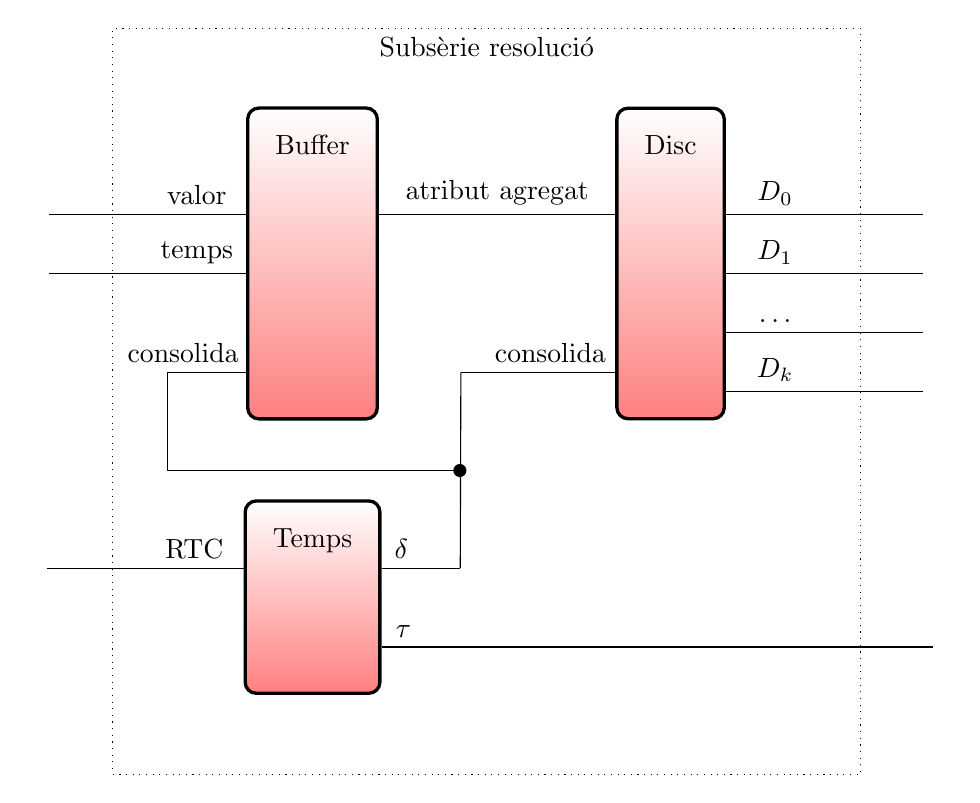
\begin{tikzpicture}
\tikzset{
    maquina/.style={rectangle,rounded corners,draw=black, 
      very thick, inner sep=1em, minimum size=3em, text centered,
      groc},
    interficie/.style={rectangle,rounded corners,draw=black, 
       inner sep=0.2em, minimum size=1em, text centered,
      verd},
    modul/.style={rectangle,rounded corners,draw=black, 
      very thick, inner sep=1em, minimum size=3em, text centered,
      roig},   
    myarrow/.style={->, >=latex', shorten >=1pt, thick},
    fletxaswitch/.style={<->, >=latex',shorten >=10pt,shorten <=10pt, thick},
    mylabel/.style={text width=7em, text centered},
    groc/.style={top color=white, bottom color=yellow!50},
    verd/.style={top color=white, bottom color=green!50},
    roig/.style={top color=white, bottom color=red!50},
  }  

  
   \node (discres) [draw, dotted, minimum width=9.5cm, text depth=9cm, rectangle] {Subsèrie resolució};



  \node[modul,text depth=3cm,below right=1cm and 1.7cm of discres.north west] (buffer) {Buffer};  

  %entrades
  \node[above left=-1.5cm and 2.5cm of buffer.north west] (buffer_valor)   {};
  \draw[-] (buffer_valor) -- (buffer_valor-|buffer.west)
   node[near end,above]{valor};

   \node[below=0.5cm of buffer_valor] (buffer_nou)   {};
   \draw[-] (buffer_nou) -- (buffer_nou-|buffer.west)
   node[near end,above]{temps};

   \node[above left=-3.5cm and 1cm of buffer.north west] (buffer_consolida) {};
   \draw[-] (buffer_consolida) -- (buffer_consolida-|buffer.west)
   node[pos=0.2,above]{consolida};

   %sortides
   \node[above right=-1.5cm and 1.5cm of buffer.north east] (buffer_dada)   {};
  \draw[-] (buffer_dada) -- (buffer_dada-|buffer.east)
   node[pos=0,above]{atribut agregat};





  \node[modul,right=3cm of buffer,text depth=3cm] (disc)   {Disc}; 

  % entrades
  \node[above left=-1.5cm and 2cm of disc.north west] (disc_valor)   {};
  \draw[-] (disc_valor) -- (disc_valor-|disc.west)
   node[near end,above]{};

  \node[above left=-3.5cm and 1.96cm of disc.north west] (disc_consolida)   {};
  \draw[-] (disc_consolida) -- (disc_consolida-|disc.west)
   node[pos=0.58,above]{consolida};

   % sortides
   \node[above right=-1.5cm and 2.5cm of disc.north east] (disc_d0)   {};
   \draw[-] (disc_d0) -- (disc_d0-|disc.east)
   node[near end,above]{$D_0$};

   \node[below=0.5cm of disc_d0] (disc_d1)   {};
  \draw[-] (disc_d1) -- (disc_d1-|disc.east)
   node[near end,above]{$D_1$};

   \node[below=0.5cm of disc_d1] (disc_d2)   {};
  \draw[-] (disc_d2) -- (disc_d2-|disc.east)
   node[near end,above]{$\dots$};

   \node[below=0.5cm of disc_d2] (disc_d3)   {};
  \draw[-] (disc_d3) -- (disc_d3-|disc.east)
   node[near end,above]{$D_k$};




  \node[modul,below=1cm of buffer,text depth=1.5cm] (temps)   {Temps}; 

  % entrades
  \node[above left=-1cm and 2.5cm of temps.north west] (temps_rtc)   {};
  \draw[-] (temps_rtc) -- (temps_rtc-|temps.west)
   node[near end,above]{RTC};

  % sortides
   \node[above right=-1cm and 1cm of temps.north east] (temps_delta)   {};
   \draw[-] (temps_delta) -- (temps_delta-|temps.east)
   node[near end,above]{$\delta$};

   \node[above right=-2cm and 7cm of temps.north east] (temps_tau)   {};
   \draw[-] (temps_tau) -- (temps_tau-|temps.east)
   node[pos=0.96,above]{$\tau$};








   %connexions
   \draw[-] (temps_delta.west) -- (disc_consolida.east); 
   
%   \node[above left=0.3cm and 1cm of temps.north west] (tau_reset)   {};
   \node[below=1cm of buffer_consolida] (tau_reset)   {};
   \draw[-*,shorten >=-2pt] (tau_reset) -- (tau_reset-|disc_consolida.east);
   \draw[-] (tau_reset.east) -- (tau_reset.east|-buffer_consolida);


 \end{tikzpicture}
 
\caption{Esquema genèric d'un disc resolució}
\label{fig:vhdl:disc-resolucio}
\end{figure}


Condicions:
\begin{itemize}
\item Àmbit: xarxes de sensors
\item No apte per processos industrials ni llaços de control, en els
  quals cal tenir totes les dades
\item Possibilitat de validació de dades del sensor (en el buffer) i
  generar avisos de funcionament incorrecte.
\item Interfície per a consulta les dades?
\end{itemize}





Estructures alternatives:
\begin{itemize}
\item timestamps absoluts: $\delta$ creats a partir de RTC
\item timestamps relatius: $\delta$ creats a partir del clock
\item timestamps creixents: l'RTC el marca el temps de la mesura
\item Memòria estàtica en comptes de volàtil. Útil per a: a) tenir dades permanents en cas d'apagada o b) per a poder consumir menys (?)   ->  tot això no seria millor fer-ho per programa (CPU) que implementat físicament (aleshores seria més reprogramable)?
\end{itemize}





Base de dades completa, conjunt de discs resolució:
\usetikzlibrary{shapes,arrows,positioning}

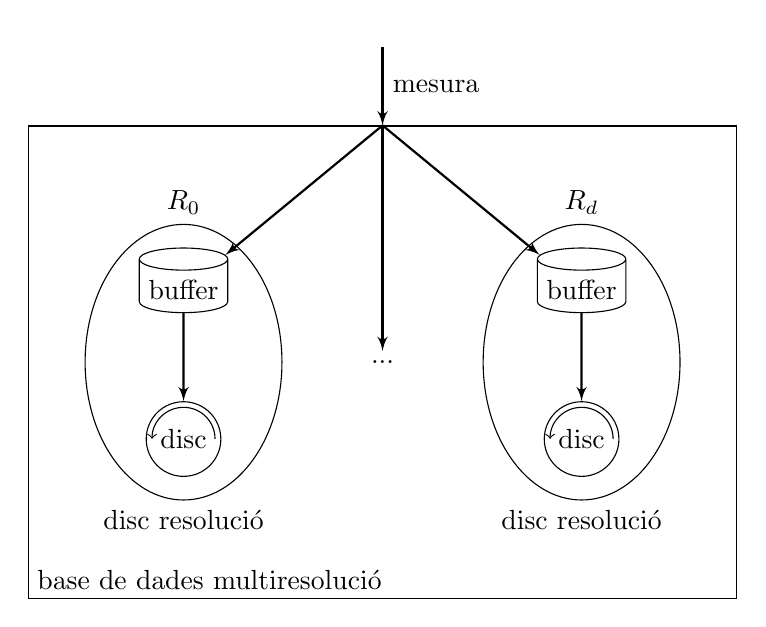
\begin{tikzpicture}
 \tikzset{
        myarrow/.style={->, >=latex',  thick},
      }
      

  \node[rectangle,draw,minimum height=6cm,minimum width=9cm] (m) {};
  \draw[shift=( m.south west)]   
  node[above right] {base de dades multiresolució};


  %discmig
  \node (m.center) (discr1) {...};

  %discr
  
  \node[ellipse,draw,minimum height=3.5cm,minimum width=2.5cm,alias=discr0] [left=of discr1] {};
  \node[above=0cm of discr0.north] {$R_0$};
  \node[below=0cm of discr0] {disc resolució};

  \node[cylinder, draw, shape border rotate=90, aspect=0.25,alias=buffer0] [below=3mm of discr0.north] {buffer};
  \node[circle, draw,alias=disc0]  [above=3mm of discr0.south] {disc} ;
  \draw [->] (disc0.center)++(.4:.4cm) arc(0:180:.4cm);
  \draw[myarrow] (buffer0.bottom) -- (disc0.north);


  %discrd

  \node[ellipse,draw,minimum height=3.5cm,minimum width=2.5cm,alias=discrd] [right=of discr1] {};
  \node[above=0cm of discrd] {$R_d$};
  \node[below=0cm of discrd] {disc resolució};

  \node[cylinder, draw, shape border rotate=90, aspect=0.25,alias=bufferd] [below=3mm of discrd.north] {buffer};
  \node[circle, draw,alias=discd]  [above=3mm of discrd.south] {disc} ;
  \draw [->] (discd.center)++(.4:.4cm) arc(0:180:.4cm);
  \draw[myarrow] (bufferd.bottom) -- (discd.north);



  %mesura 
  \node[above=1cm of m.north] (m0) {};

  \draw[myarrow] (m0) -- (m.north) 
  node[right,midway] {mesura};

  \draw[myarrow] (m.north) -- (buffer0);
  \draw[myarrow] (m.north) -- (bufferd);
  \draw[myarrow] (m.north) -- (discr1);

\end{tikzpicture}




Base de dades amb discs resolució enllaçats:

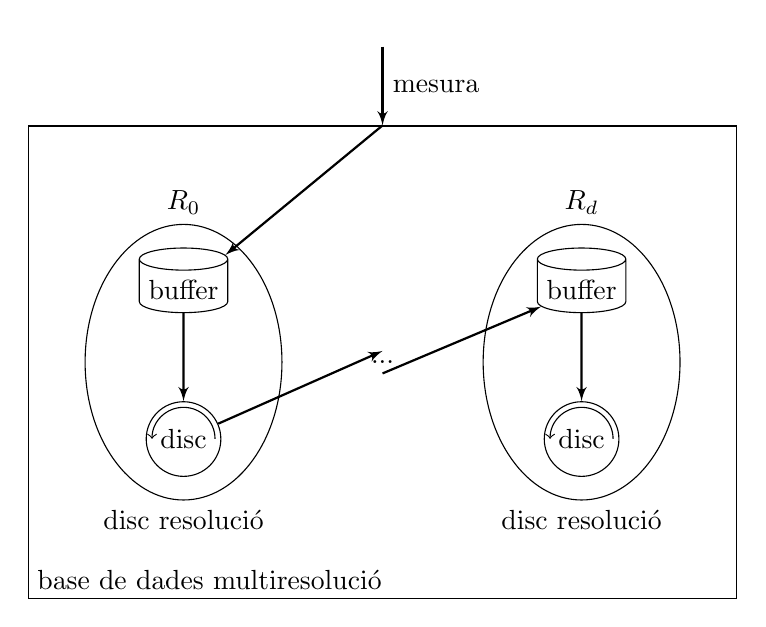
\begin{tikzpicture}
 \tikzset{
        myarrow/.style={->, >=latex',  thick},
      }
      

  \node[rectangle,draw,minimum height=6cm,minimum width=9cm] (m) {};
  \draw[shift=( m.south west)]   
  node[above right] {base de dades multiresolució};


  %discmig
  \node (m.center) (discr1) {...};

  %discr
  
  \node[ellipse,draw,minimum height=3.5cm,minimum width=2.5cm,alias=discr0] [left=of discr1] {};
  \node[above=0cm of discr0.north] {$R_0$};
  \node[below=0cm of discr0] {disc resolució};

  \node[cylinder, draw, shape border rotate=90, aspect=0.25,alias=buffer0] [below=3mm of discr0.north] {buffer};
  \node[circle, draw,alias=disc0]  [above=3mm of discr0.south] {disc} ;
  \draw [->] (disc0.center)++(.4:.4cm) arc(0:180:.4cm);
  \draw[myarrow] (buffer0.bottom) -- (disc0.north);


  %discrd

  \node[ellipse,draw,minimum height=3.5cm,minimum width=2.5cm,alias=discrd] [right=of discr1] {};
  \node[above=0cm of discrd] {$R_d$};
  \node[below=0cm of discrd] {disc resolució};

  \node[cylinder, draw, shape border rotate=90, aspect=0.25,alias=bufferd] [below=3mm of discrd.north] {buffer};
  \node[circle, draw,alias=discd]  [above=3mm of discrd.south] {disc} ;
  \draw [->] (discd.center)++(.4:.4cm) arc(0:180:.4cm);
  \draw[myarrow] (bufferd.bottom) -- (discd.north);



  %mesura 
  \node[above=1cm of m.north] (m0) {};

  \draw[myarrow] (m0) -- (m.north) 
  node[right,midway] {mesura};

  \draw[myarrow] (m.north) -- (buffer0);
  \draw[myarrow] (discr1.south) -- (bufferd);
  \draw[myarrow] (disc0) -- (discr1.north);

\end{tikzpicture}









% \begin{tikzpicture}[circuit logic IEC,
%   every circuit symbol/.style={
%     logic gate IEC symbol color=black,
%     fill=blue!20,draw=blue,very thick}]
%   \matrix[column sep=7mm]
%   {
%     \node (i0) {0}; &
%     & \\
%     & \node [and gate] (a1) {}; & \\
%     \node (i1) {0}; &
%     & \node [or gate] (o) {};\\
%     & \node [nand gate] (a2) {}; & \\
%     \node (i2) {1}; &
%     & \\
%   };
%   \draw (i0.east) -- ++(right:3mm) |- (a1.input 1);
%   \draw (i1.east) -- ++(right:3mm) |- (a1.input 2);
%   \draw (i1.east) -- ++(right:3mm) |- (a2.input 1);
%   \draw (i2.east) -- ++(right:3mm) |- (a2.input 2);
%   \draw (a1.output) -- ++(right:3mm) |- (o.input 1);
%   \draw (a2.output) -- ++(right:3mm) |- (o.input 2);
%   \draw (o.output) -- ++(right:3mm);
% \end{tikzpicture}








% \def\degr{${}^\circ$}
% \begin{tikztimingtable}
%   Clock 128\,MHz 0\degr    & H   12{2C} G \\ % ends with edge
%   Clock 128\,MHz 90\degr   & [C] 12{2C} C \\ % starts with edge
%   Clock 128\,MHz 180\degr  & C   12{2C} G \\ % ends with edge
%   Clock 128\,MHz 270\degr  &     12{2C} C \\
% \end{tikztimingtable}





\subsection{Possibles aplicacions}

Exemple d'aparell encastat molt petit, per exemple un aparell que
s'hagi de posar dins del cos per a mesurar la temperatura, a on hi ha
molt poc espai disponible i només permet emmagatzemar 100 dades. Es
poden desar 100 valors cada hora = 4 dies, o bé es pot aplicar una
solució de multiresolució i desa 75 valors cada hora = 2 dies i 25
valors cada dia = 25 dies. Així si no s'és a temps de recuperar les
dades en quatre dies sempre hi haurà alguna informació.

Exemple de la implementació de circuits integrats en materials molt prims i doblegables.




Bàsicament en les implementacions a baix nivell d'un SGSTM tenim dues opcions:

\begin{itemize}
\item implementar-ho amb llenguatge de baix nivell (assemblador, C) en un microcontrolador. Aquesta seria la manera típica perquè dóna molta flexibilitat: es pot reconfigurar l'esquema de multiresolució quan es vulgui, es poden utilitzar les operacions que es vulgui, canviar la mida, etc. 

\item implementar-ho amb hardware, per exemple dissenyar amb
  VHDL. Inconvenients: gens flexible (un cop implementat no es pot
  canviar), difícil de fer genèric (no es pot trobar un circuit que
  serveixi per a fer varis càlculs, per això caldria un
  microcontrolador). Avantatges: es pot compactar i encastar en
  llocs petits, estructures de càlcul paral·leles (la feina no recau
  en el microcontrolador), bases de dades distribuïdes. Per tant es fa
  difícil pensar de vendre BDM genèriques hardware però sí que es
  poden pensar algunes possibles aplicacions que només serien
  exclusives de hardware:

  \begin{itemize}
  \item Sensors inte\l.ligents o totalment encastats. Actualment es
    dissenyen sensors acompanyats de circuits digitals, tot encastat
    en un xip petit. Fan filtratge dels senyal, tenen un bus de
    comunicació senzill amb el controlador (I2C, 1-Wire, SPI, etc.), el
    controlador pot indicar quan s'ha d'iniciar la captura d'un no
    valor, s'emmagatzema el darrer valor capturat i el controlador el
    consulta quan vol, poden establir uns llindars d'alarma... Així
    doncs aquests sensors només emmagatzemen el darrer valor, es
    podria proposar que emmagatzemessin amb esquema multiresolució, el
    qual hauria de ser una mica configurable per exemple els períodes
    de consolidació. No obstant això, la configuració seria molt poc
    flexible i si es necessiten càlculs més complicats sempre és
    millor seguir amb l'esquema habitual del microcontrolador captura
    la dada i ell gestiona els càlculs. Ara bé, també es pot entendre
    el sensor inte\l.ligent com que forma part d'una base de dades
    distribuïda i ell té una part de l'emmagatzematge. 
    
  \item Esquema multiresolució encastat en perifèrics per a monitorar
    el seu funcionament: en una impressora en els comptadors
    d'impressions, en una antena de comunicació sense fils en els
    comptadors de bytes transmesos o la potència transmesa, etc.

  \item Implementació de circuits integrats en llocs mai vistos:
    materials molt prims i doblegables. Aquí segurament hi ha
    problemes de la mida dels circuits que es poden implementar, per
    tant poder-hi disposar d'esquemes multiresolució aniria bé.

  \item Possibilitat de disseny de FPGA casolans. Si mai això fos
    possible (sembla que ja és possible: exemple de FPGA a la
    raspberry, System-on-Chip (SoC)), els sensors intel·ligents o
    totalment encastats prendrien molt sentit ja que serien
    reconfigurables o que fos molt barat implementar en hardware un
    circuit i llençar-lo quan es volgués canviar de configuració. Això
    llavors encaixaria amb construir un xip per blocs: hi poso un bloc
    de comunicacions, un bloc de tal i un bloc de base de dades
    multiresolució amb tal esquema. Tot i així, sembla que en els SoC
    la idea és implementar-ho com a microcontrolador i fins i tot
    implementar-hi sistemes operatius.

  \end{itemize}


\end{itemize}

En l'àmbit, no es veu clara la implementació de coses en VHDL. Sembla que es desaprofitar recursos perquè la feina ja la pot fer el microcontrolador. Potser l'aplicació útil i que s'ha de destacar és quan en els xips integrats no hi ha microcontrolador com poder-hi posar una base de dades?


%%% Local Variables:
%%% TeX-master: "main"
%%% End:

\chapter{Exemple}
\label{sec:implementacions:exemple}

En aquest capítol mostrem un exemple de base de dades multiresolució
aplicada a una sèrie temporal real amb dades massives.  

\todo{}
We use Pytsms and
RoundRobinson implementations in order to create a \acro{MTSDB} and
to query it.

També fem servir roundrobindoop i reltsms?


Passos:

\begin{enumerate}
\item Descrivim la sèrie temporal original.
\item Proposem un esquema de multiresolució.
\item Computem la consolidació de la sèrie temporal amb l'esquema proposat. \todo{amb diferents implementacions}
\item Avaluem els resultats.
\item Comparem les diferents implementacions.
\end{enumerate}


En les computacions hem utilitzat els reals estesos,
$\glssymbol{not:Rb}$, com a domini del temps segons l'estàndard d'Hora
Unix (\seeref{sec:sgst:temps}). Això no obstant, per a facilitar-ne la
comprensió, en els exemples mostrem el domini del temps amb el format
de calendari d'\gls{UTC}.




\section{Dades}


Les dades provenen d'un sistema de monitoratge de temperatura en una
xarxa de sensors distribuïts \parencite{alippi10}, en aquest cas ens
centrem en les dades d'un sensor.

Les dades es mostren a la \autoref{fig:exemple:original}.  És una
sèrie temporal adquirida durant un període d'un any i mig, des del 29
d'abril del 2010 fins al 18 d'octubre del 2011. En aquest gràfic, la
sèrie temporal es mostra interpolant linealment les mesures, és a dir
amb el mètode de representació \gls{foh}.  
%
En total hi ha $146.709$
mesures emmagatzemades de la temperatura que va adquirir el sensor, en
graus Kelvin (K), cada 2 minuts tot i que de forma irregular.  Tot i
així en el gràfic només mostrem 466 punts, escollits mitjançant una
delmació amb una resolució d'un dia, ja que de totes maneres una
resolució superior és imperceptible.  En el gràfic d'aquesta sèrie
temporal destaquen alguns períodes en què hi manquen dades i alguns en
què hi ha observacions aberrants.


\begin{figure}[tp]
  \centering
  \usetikzlibrary{dateplot}    
\begin{tikzpicture}
    \begin{axis}[
        date coordinates in=x,
%        xticklabel={\pgfcalendar{tickcal}{\tick}{\tick}{\pgfcalendarshorthand{m}{.}}},
        xticklabel={\pgfcalendarmonthshortname{\month} \year},
        xticklabel style= {rotate=15,anchor=east},
        xlabel=Time,
        ylabel=Temperature (K),
        ymax = 320,
        clip=false,
        y filter/.code = { \pgfmathparse{(#1>320)*322+(#1<320)*#1}},
        ]
       \addplot[blue] file {dades/matriu0.originalbyday.dat};

%      \node[right] at (axis cs:2011-10-12,330) {\footnotesize(2938)};
       \node (break) at (axis cs:2011-10-02,318)[inner sep=0pt,minimum width=0.75em, minimum height=0.5ex,fill=white] {};
    \draw [fill=red,color=blue] (break.north east) -- (break.north west) (break.south west) -- (break.south east);



  \end{axis}
\end{tikzpicture}



%%% Local Variables:
%%% TeX-master: "../main"
%%% ispell-local-dictionary: "british"
%%% End:

  \caption{Sèrie temporal d'un sensor de temperatura}
  \label{fig:exemple:original}
\end{figure}





\section{Esquema de multiresolució}

Dissenyem un esquema de multiresolució per a la sèrie temporal.
Aquest esquema resumeix la sèrie temporal amb més resolució per als
temps recents i amb menys resolució per als temps antics.



El cronograma de l'esquema de multiresolució es mostra a la
\autoref{fig:exemple:cronograma}, en què cada resolució té un color
diferent. Té la mateixa estructura que el cronograma periòdic definit
a la \autoref{fig:model:cronograma-simplificat} però amb els valors
particularitzats per a aquest exemple.  De més a menys resolució,
l'esquema és el següent:



\begin{figure}[tp]
  \centering
  %mrd.afegeix_disc(h5,24,mitjana,zero)
%mrd.afegeix_disc(d2,20,mitjana,zero)
%mrd.afegeix_disc(d15,12,mitjana,zero)
%mrd.afegeix_disc(d50,12,mitjana,zero)
\tiny
\begin{center}
%\begin{multicols}{4} 


    \begin{picture}(14,12)(-7,-6)
    \put(0,-1){\makebox(0,0)[c]{{\color{blue}50 days}}}
      \put(0,0){\circle{10}}
      \put(5,0){\circle{0.8}}
      \put(4.33,2.5){\circle{0.8}}
      \put(2.5,4.33){\circle{0.8}}
      \put(0,5){\circle{0.8}}
      \put(-2.5,4.33){\circle{0.8}}   
      \put(-4.33,2.5){\circle{0.8}}
      \put(-5,0){\circle{0.8}}
      \put(-4.33,-2.5){\circle{0.8}}
      \put(-2.5,-4.33){\circle{0.8}} 
      \put(0,-5){\circle{0.8}}
      \put(2.5,-4.33){\circle{0.8}} 
      \put(4.33,-2.5){\circle{0.8}}
      \put(0,0){\vector(0,1){5}}
      \put(0,0){\oval(5,5)[t]}
      \put(-2.5,0){\makebox(0,0)[c]{$\vee$}}
    \end{picture}
%
    \begin{picture}(14,12)(-7,-6)
    \put(0,-1){\makebox(0,0)[c]{{\color{brown}15 days}}}
      \put(0,0){\circle{10}}
      \put(5,0){\circle{0.8}}
      \put(4.33,2.5){\circle{0.8}}
      \put(2.5,4.33){\circle{0.8}}
      \put(0,5){\circle{0.8}}
      \put(-2.5,4.33){\circle{0.8}}   
      \put(-4.33,2.5){\circle{0.8}}
      \put(-5,0){\circle{0.8}}
      \put(-4.33,-2.5){\circle{0.8}}
      \put(-2.5,-4.33){\circle{0.8}} 
      \put(0,-5){\circle{0.8}}
      \put(2.5,-4.33){\circle{0.8}} 
      \put(4.33,-2.5){\circle{0.8}}
      \put(0,0){\vector(0,1){5}}
      \put(0,0){\oval(5,5)[t]}
      \put(-2.5,0){\makebox(0,0)[c]{$\vee$}}
    \end{picture}
%
    \begin{picture}(14,12)(-7,-6)
    \put(0,-1){\makebox(0,0)[c]{{\color{red}2 days}}}
      \put(0,0){\circle{10}}
      %\put(5,0){\circle{0.8}}
      \put(4.82,1.29){\circle{0.8}}
      \put(4.33,2.5){\circle{0.8}}
     \put(3.5,3.5){\circle{0.8}}
      \put(2.5,4.33){\circle{0.8}}
      \put(1.29,4.82){\circle{0.8}}
      %\put(0,5){\circle{0.8}}
      \put(-1.29,4.82){\circle{0.8}}
      \put(-2.5,4.33){\circle{0.8}}
       \put(-3.5,3.5){\circle{0.8}} 
      \put(-4.33,2.5){\circle{0.8}}
    \put(-4.82,1.29){\circle{0.8}}
      %\put(-5,0){\circle{0.8}}
    \put(-4.82,-1.29){\circle{0.8}}
      \put(-4.33,-2.5){\circle{0.8}}
      \put(-3.5,-3.5){\circle{0.8}} 
      \put(-2.5,-4.33){\circle{0.8 } } 
      \put(-1.29,-4.82){\circle{0.8 }}
      % \put(0,-5){\circle{0.8 }}
     \put(1.29,-4.82){\circle{0.8 }}
      \put(2.5,-4.33){\circle{0.8}}
      \put(3.5,-3.5){\circle{0.8}} 
      \put(4.33,-2.5){\circle{0.8}}
  \put(4.82,-1.29){\circle{0.8}}
      \put(0,0){\vector(0,1){5}}
      \put(0,0){\oval(5,5)[t]}
      \put(-2.5,0){\makebox(0,0)[c]{$\vee$}}
    \end{picture}
%
    \begin{picture}(14,12)(-7,-6)
    \put(0,-1){\makebox(0,0)[c]{{\color{cyan}5 hours}}}
      \put(0,0){\circle{10}}
      \put(5,0){\circle{0.8}}
      \put(4.82,1.29){\circle{0.8}}
      \put(4.33,2.5){\circle{0.8}}
     \put(3.5,3.5){\circle{0.8}}
      \put(2.5,4.33){\circle{0.8}}
      \put(1.29,4.82){\circle{0.8}}
      \put(0,5){\circle{0.8}}
      \put(-1.29,4.82){\circle{0.8}}
      \put(-2.5,4.33){\circle{0.8}}
       \put(-3.5,3.5){\circle{0.8}} 
      \put(-4.33,2.5){\circle{0.8}}
    \put(-4.82,1.29){\circle{0.8}}
      \put(-5,0){\circle{0.8}}
    \put(-4.82,-1.29){\circle{0.8}}
      \put(-4.33,-2.5){\circle{0.8}}
      \put(-3.5,-3.5){\circle{0.8}} 
      \put(-2.5,-4.33){\circle{0.8 } } 
      \put(-1.29,-4.82){\circle{0.8 }}
\put(0,-5){\circle{0.8 }}
     \put(1.29,-4.82){\circle{0.8 }}
      \put(2.5,-4.33){\circle{0.8}}
      \put(3.5,-3.5){\circle{0.8}} 
      \put(4.33,-2.5){\circle{0.8}}
  \put(4.82,-1.29){\circle{0.8}}
      \put(0,0){\vector(0,1){5}}
      \put(0,0){\oval(5,5)[t]}
      \put(-2.5,0){\makebox(0,0)[c]{$\vee$}}
    \end{picture}


%\end{multicols}

\vspace{-10pt}

\setlength{\unitlength}{900sp}
\begin{picture}(14460,5066)(7322,-7148)
\thinlines
{\color[rgb]{0,0,0}\put(7300,-6271){\line( 0,-1){386}}
}%
{\color[rgb]{0,0,0}\put(7782,-6271){\line( 0,-1){386}}
}%
{\color[rgb]{0,0,0}\put(8263,-6271){\line( 0,-1){386}}
}%
{\color[rgb]{0,0,0}\put(8745,-6271){\line( 0,-1){386}}
}%
{\color[rgb]{0,0,0}\put(9227,-6271){\line( 0,-1){386}}
}%
{\color[rgb]{0,0,0}\put(9709,-6271){\line( 0,-1){386}}
}%
{\color[rgb]{0,0,0}\put(10191,-6271){\line( 0,-1){386}}
}%
{\color[rgb]{0,0,0}\put(10673,-6271){\line( 0,-1){386}}
}%
{\color[rgb]{0,0,0}\put(11155,-6271){\line( 0,-1){386}}
}%
{\color[rgb]{0,0,0}\put(11637,-6271){\line( 0,-1){386}}
}%
{\color[rgb]{0,0,0}\put(12119,-6271){\line( 0,-1){386}}
}%
{\color[rgb]{0,0,0}\put(12600,-6271){\line( 0,-1){386}}
}%
{\color[rgb]{0,0,0}\put(13082,-6271){\line( 0,-1){386}}
}%
{\color[rgb]{0,0,0}\put(13564,-6271){\line( 0,-1){386}}
}%
{\color[rgb]{0,0,0}\put(14046,-6271){\line( 0,-1){386}}
}%
{\color[rgb]{0,0,0}\put(14528,-6271){\line( 0,-1){386}}
}%
{\color[rgb]{0,0,0}\put(15010,-6271){\line( 0,-1){386}}
}%
{\color[rgb]{0,0,0}\put(15492,-6271){\line( 0,-1){386}}
}%
{\color[rgb]{0,0,0}\put(15974,-6271){\line( 0,-1){386}}
}%
{\color[rgb]{0,0,0}\put(16456,-6271){\line( 0,-1){386}}
}%
{\color[rgb]{0,0,0}\put(16938,-6271){\line( 0,-1){386}}
}%
{\color[rgb]{0,0,0}\put(17419,-6271){\line( 0,-1){386}}
}%
{\color[rgb]{0,0,0}\put(17901,-6271){\line( 0,-1){386}}
}%
{\color[rgb]{0,0,0}\put(18383,-6271){\line( 0,-1){386}}
}%
{\color[rgb]{0,0,0}\put(18865,-6271){\line( 0,-1){386}}
}%
{\color[rgb]{0,0,0}\put(19347,-6271){\line( 0,-1){386}}
}%
{\color[rgb]{0,0,0}\put(19829,-6271){\line( 0,-1){386}}
}%
{\color[rgb]{0,0,0}\put(20311,-6271){\line( 0,-1){386}}
}%
{\color[rgb]{0,0,0}\put(20793,-6271){\line( 0,-1){386}}
}%
{\color[rgb]{0,0,0}\put(21275,-6271){\line( 0,-1){386}}
}%
{\color[rgb]{0,0,0}\put(7300,-6271){\line( 0,-1){1157}}
}%
{\color[rgb]{0,0,0}\put(9709,-6271){\line( 0,-1){1157}}
}%
{\color[rgb]{0,0,0}\put(12119,-6271){\line( 0,-1){1157}}
}%
{\color[rgb]{0,0,0}\put(14528,-6271){\line( 0,-1){1157}}
}%
{\color[rgb]{0,0,0}\put(16938,-6271){\line( 0,-1){1157}}
}%
{\color[rgb]{0,0,0}\put(19347,-6271){\line( 0,-1){1157}}
}%
{\color[rgb]{0,0,0}\put(21756,-6271){\line( 0,-1){1157}}
}%
{\color[rgb]{0,0,0}\put(7300,-6271){\line( 1, 0){14456}}
}%

\put(7322,-6271){\line( 0,1){3000}}
\put(21756,-7783){\makebox(0,0)[b]{now}}%
\put(7322,-7783){\makebox(0,0)[b]{600 days back}}%

\color{blue}
\put(21782,-5928){\line( -1,0){14460}}
\put(21782,-5928){\line( 0,1){779}}
\put(21782,-5149){\line( -1,0){14460}}
\put(7322,-5928){\line( 0,1){779}}
\put(14530,-5450){\makebox(0,0)[c]{600 days}}

\color{brown}
\put(21782,-5149){\line( 0,1){779}}
\put(21782,-4370){\line( -1,0){4438}}
\put(17344,-5149){\line( 0,1){779}}
\put(19563,-4800){\makebox(0,0)[c]{180 days}}

\color{red}
\put(21782,-4370){\line( 0,1){779}}
\put(21782,-3591){\line( -1,0){964}}
\put(20818,-4370){\line( 0,1){779}}
\put(21300,-3950){\makebox(0,0)[c]{40d}}

\color{cyan}
\put(21782,-3591){\line( 0,1){779}}
\put(21782,-2812){\line( -1,0){120}}
\put(21661,-3591){\line( 0,1){779}}
\put(21300,-3201){\makebox(0,0)[c]{5d}}
\end{picture}%


\normalsize

\end{center}
  \caption{Cronograma de l'esquema de multiresolució}
  \label{fig:exemple:cronograma}
\end{figure}

\begin{enumerate}
\item Es consolida una mesura cada 5 hores en un disc amb capacitat de
  24 mesures. Per tant, en total aquesta resolució emmagatzema
  informació durant 5 dies.

\item Es consolida una mesura cada 2 dies en un disc amb capacitat de
  20 mesures. Per tant, s'emmagatzema durant 40 dies.

\item Es consolida una mesura cada 15 dies en un disc amb capacitat de
  12 mesures.  Per tant, s'emmagatzema durant 180 dies.

\item Es consolida una mesura cada 50 dies en un disc amb capacitat de
  12 mesures.  Per tant, s'emmagatzema durant 600 dies.

\end{enumerate}



Aquest esquema està dissenyat per mostrar diferents paràmetres de la
multiresolució. Així el criteri escollit és el de visualitzar algunes
resolucions de la sèrie temporal original, la qual té un període de
mostreig irregular de 2 minuts, des de la resolució cada 5 hores fins
a la resolució cada 50 dies. També s'ha escollit per a mantenir uns
lapses de temps repartits, des del lapse de 600 dies que emmagatzema
tota la sèrie temporal original fins al de 5 dies que només conté una
informació molt recent.


Com a funció d'agregació d'atributs utilitzem la mitjana de la família
\gls{zohe} (\seeref{def:sgstm:agregadorszohe}) per a totes les
resolucions. A més, per a mostrar diferents maneres d'usar els
agregadors, utilitzem el màxim de la família \gls{zohe} però només per
a les darreres resolucions.


De manera simplificada, iniciem la consolidació de totes les
resolucions al mateix instant de temps, que notem amb $\tau_0$. Com ja
hem dit, les dades originals s'inicien el 29 d'abril del 2010, per
tant un $\tau_0=$ 1 de gener de 2010 és raonable.


Així doncs, l'expressió de l'esquema de multiresolució en termes de la \autoref{def:sgstm:esquema}, i enumerant cada resolució,  és
\begin{align*}
e = \{ &\\ 
&(\delta_1=5 \text{ h},f_1=\glssymbol{not:sgstm:meanzohe},k_1=24,\tau_1=\tau_0),\\
&(\delta_2=2 \text{ d},f_2=\glssymbol{not:sgstm:meanzohe},k_2=20,\tau_2=\tau_0),\\
&(\delta_3=15 \text{ d},f_3=\glssymbol{not:sgstm:meanzohe},k_3=12,\tau_3=\tau_0),\\
&(\delta_4=50 \text{ d},f_4=\glssymbol{not:sgstm:meanzohe},k_4=12,\tau_4=\tau_0),\\
&(\delta_{3b}=15 \text{ d},f_{3b}=\glssymbol{not:sgstm:maxzohe},k_{3b}=12,\tau_{3b}=\tau_0),\\
&(\delta_{4b}=50 \text{ d},f_{4b}=\glssymbol{not:sgstm:maxzohe},k_{4b}=12,\tau_{4b}=\tau_0),\\
\}&
\end{align*}

% \begin{align*}
% e = ( & (\delta,f,k,\tau), \{  \\ 
% &(5 \text{ h},\glssymbol{not:sgstm:meanzohe},24,\tau_0),\\
% &(2 \text{ d},\glssymbol{not:sgstm:meanzohe},20,\tau_0),\\
% &(15 \text{ d},\glssymbol{not:sgstm:meanzohe},12,\tau_0),\\
% &(50 \text{ d},\glssymbol{not:sgstm:meanzohe},12,\tau_0),\\
% &(15 \text{ d},\glssymbol{not:sgstm:maxzohe},12,\tau_0),\\
% &(50 \text{ d},\glssymbol{not:sgstm:maxzohe},12,\tau_0),\\
% \})&
% \end{align*}

Com que els atributs de mitjana i màxim comparteixen les dues darreres
resolucions, les anomenem amb el mateix número però marcant amb una
$b$ les de màxim.  En total, sumant les capacitats de cada disc,
s'emmagatzemen $24+20+12+12+12+12=92$ mesures.







\section{Resultats de la consolidació}

En un \gls{SGSTM}, consolidem la sèrie temporal original amb l'esquema
de multiresolució proposat. Del resultat, podem fer-ne les dues consultes bàsiques (\seeref{sec:sgstm:consultes}):

\begin{enumerate}
\item Les consultes \glssymbol{not:sgstm:seriedisc} per a obtenir les
  subsèries temporals que han quedat consolidades a cada subsèrie
  resolució.
\item Les consultes \glssymbol{not:sgstm:serietotal} per a obtenir la sèrie
  temporal total per a cada atribut.
\end{enumerate}


En primer lloc, a la \autoref{fig:exemple:4mrd} es mostren totes les
subsèries resolució consolidades. Cada gràfic correspon a una consulta
possible de \glssymbol{not:sgstm:seriedisc}, tot i que les resolucions
que només difereixen en l'atribut es mostren en el mateix gràfic.
Aquest és el cas de les dues darreres resolucions que comparteixen els
mateixos paràmetres llevat de la funció d'agregació d'atributs: en
blau es mostra l'atribut de \glssymbol{not:sgstm:meanzohe} i en
taronja el de \glssymbol{not:sgstm:maxzohe}.  El títol de cada gràfic
indica la subsèrie resolució i els paràmetres de pas de consolidació i
de cardinal màxim.


\begin{figure}[tp]
  \centering
  % \tikzset{
  %   every picture/.style={scale=0.7},
  % }
  
  \begin{tikzpicture}[scale=0.6, every node/.style={transform shape}]
    \begin{axis}[
        multiresoluciodate,
        title={$R_1$: 5h $|24|$},
        xticklabel={\day--\hour:\minute},
        clip=false,
        ]
       \addplot[const plot mark right, blue] table[col sep=comma] {imatges/exemple/dades-matriu0/R18000mean_zohe.csv};
     \node[left] at (axis cs:2011-10-19,274) {\footnotesize oct.~2011};
  \end{axis}
\end{tikzpicture}
%
  \begin{tikzpicture}[scale=0.6, every node/.style={transform shape}]
    \begin{axis}[
        multiresoluciodate,
        title={$R_2$: 2d $|20|$},
        xticklabel={\day~\pgfcalendarmonthshortname{\month}},
        clip=false,
        ]
       \addplot[const plot mark right, blue] table[col sep=comma] {imatges/exemple/dades-matriu0/R172800mean_zohe.csv};
     \node[left] at (axis cs:2011-10-21,279) {\footnotesize 2011};
  \end{axis}
\end{tikzpicture}
%
  \begin{tikzpicture}[scale=0.6, every node/.style={transform shape}]
    \begin{axis}[
        multiresoluciodate,
        title={$R_3$: 15d $|12|$},
        xticklabel={\day~\pgfcalendarmonthshortname{\month}},
        y filter/.code = { \pgfmathparse{(#1>320)*330+(#1<320)*#1}},
        ymax = 320,
        clip=false,
        ]

       \addplot[const plot mark right, blue] table[col sep=comma] {imatges/exemple/dades-matriu0/R1296000mean_zohe.csv};

      \addplot[const plot mark right, orange] table[col sep=comma] {imatges/exemple/dades-matriu0/R1296000maximum_zohe.csv};

      \node[right] at (axis cs:2011-10-07,330) {\footnotesize(2938)};
       \node (break) at (axis cs:2011-09-23,325)[inner sep=0pt,minimum width=0.75em, minimum height=0.5ex,fill=white] {};
    \draw [fill=red,color=orange] (break.north east) -- (break.north west) (break.south west) -- (break.south east);

     \node[left] at (axis cs:2011-10-27,273) {\footnotesize 2011};

  \end{axis}
\end{tikzpicture}
%
\begin{tikzpicture}[scale=0.6, every node/.style={transform shape}]
    \begin{axis}[
        multiresoluciodate,
        xticklabel={\pgfcalendarmonthshortname{\month}~\year},
        title={$R_4$: 50d $|12|$},
        xlabel={Temps (UTC)},
%        ylabel={Temperatura (K)},
        ymax = 320,
        clip=false,
%v1.6     restrict y to domain=0:320,
        y filter/.code = { \pgfmathparse{(#1>320)*330+(#1<320)*#1}},
        ]

       \addplot[const plot mark right, blue] table[col sep=comma] {imatges/exemple/dades-matriu0/R4320000mean_zohe.csv};
       \addlegendentry{mitjana};

       \addplot[const plot mark right, orange] table[col sep=comma] {imatges/exemple/dades-matriu0/R4320000maximum_zohe.csv};
       \addlegendentry{màxim};

       \node[right] at (axis cs:2011-10-12,330) {\footnotesize(2938)};
       \node (break) at (axis cs:2011-08-24,325)[inner sep=0pt,minimum width=0.75em, minimum height=0.5ex,fill=white] {};
    \draw [fill=red,color=orange] (break.north east) -- (break.north west) (break.south west) -- (break.south east);

  \end{axis}
\end{tikzpicture}




%%% Local Variables:
%%% TeX-master: "../../main"
%%% End:

  \caption{Subsèries resolució emmagatzemades a la base de dades}
  \label{fig:exemple:4mrd}
\end{figure}

Cada sèrie temporals totals es
mostra amb el mètode de representació \gls{zohe}, car s'han
consolidat amb funcions d'agregació basades en aquest mètode.
\todo{revisar}

  Each time series is plotted
% with \zohe{} representation function $S(t)^\zohe{}$. Time axis has
% \acro{UTC} units rounded to nearest time points and temperature axis
% has Kelvin units. Outlayers are marked as discontinuities, for
% instance see fourth plot's 2938 K maximum.

% In all the four plots, we can see that mean aggregate function has
% filled missing data and filtered outlayer observations. This is due
% to the aggregate function coming from a \zohe{} interpretation.



En segon lloc,

% Figure~\ref{fig:exemple:4mrdtot} shows the $\totalseries$
% queries for the mean$^{\zohe}$ aggregate function resolution and for
% the maximum$^{\zohe}$ resolution.  Each resulting time series is
% plotted interpolating linearly its measures, note that this linearly
% visualisation seems right time displaced as time series comes from a
% \zohe{} aggregation.  Comparing this figure with the original series
% in Figure~\ref{fig:exemple:original}, we observe that it resembles an
% incremental low-pass filter because we applied mean aggregation while
% the maximum aggregation resembles an envelope function.


En gris es mostra la sèrie temporal original amb el mètode de
representació \gls{foh}. En canvi, les sèries temporals totals es
mostren amb el mètode de representació \gls{zohe}.

\begin{figure}[tp]
  \centering
  %\tikzset{every picture/.style={scale=0.8}}
  \usetikzlibrary{dateplot}  
%\usetikzlibrary{pgfplots.groupplots}

\pgfplotsset{
   petit/.style={
        ylabel=Temperature (K),
%        width=\textwidth,
%        height=3.5cm,
        legend style={font=\footnotesize},
        tick label style={font=\footnotesize},
        label style={font=\tiny},
        title style={font=\small,below, anchor=north,fill=white},
        xticklabel style= {rotate=15,anchor=east},
%        every axis title shift=0pt,
%        max space between ticks=15,
        every mark/.append style={mark size=6},
        major tick length=0.1cm,
        minor tick length=0.066cm,
        very thin,
        every axis legend/.append style={
          at={(1,0.02)},
          anchor=south east,
          draw = none},
        legend columns = 4,
    }
}

\begin{tikzpicture}
    \begin{axis}[
        petit,
        date coordinates in=x,
        xticklabel={\pgfcalendarmonthshortname{\month} \year},
        xlabel=Time (UTC),
%        unbounded coords=jump, %v>1.4
%        unbounded coords=discard, %v>1.4
        ymax = 320,
        clip=false,
%v1.6     restrict y to domain=0:320,
        y filter/.code = { \pgfmathparse{(#1>320)*330+(#1<320)*#1}},
        ]

       \addplot[black!15] file {dades/matriu0.originalbyday.dat};
       \addlegendentry{original};

       \addplot[blue] table[col sep=comma] {dades/mrdb-matriu0/union1.csv};
       \addlegendentry{mean};

       \addplot[orange] table[col sep=comma] {dades/mrdb-matriu0/union0.csv};
       \addlegendentry{max};

%       \node[right] at (axis cs:2011-10-12,330) {\mbox{(2938)}};
       \node (break) at (axis cs:2011-09-25,325)[inner sep=0pt,minimum width=0.9em, minimum height=0.4ex,fill=white] {};
    \draw [fill=red,color=orange] (break.north east) -- (break.north west) (break.south west) -- (break.south east);


  \end{axis}
\end{tikzpicture}
%http://tex.stackexchange.com/questions/46422/axis-break-in-pgfplots

%http://tex.stackexchange.com/questions/52409/insert-a-separate-mark-inside-a-pgfplots-graph



%%% Local Variables:
%%% TeX-master: "../main"
%%% ispell-local-dictionary: "british"
%%% End:

  \caption{Comparació de la sèrie temporal original amb la sèrie temporal total de la multiresolució per als atributs de mitjana i màxim \gls{zohe}}
  \label{fig:exemple:4mrdtot}
\end{figure}

\todo{alerta! s'ha d'utilitzar la concatenació temporal ZOHE, sinó el màxim queda malament en el punt de concatenació}





\begin{figure}[tp]
  \centering
  %\tikzset{every picture/.style={scale=0.8}}
  \begin{tikzpicture}
    \begin{axis}[
        timeseriesdate,
        width=0.8\textwidth,
        xticklabel={\pgfcalendarmonthshortname{\month}~\year},
        xlabel={Temps (\acrshort{UTC})},
        ylabel={Temperatura (K)},
        ymax = 320,
        clip=false,
%v1.6     restrict y to domain=0:320,
        y filter/.code = { \pgfmathparse{(#1>320)*325+(#1<320)*#1}},
        ]

       \addplot[black!15] file {imatges/exemple/matriu0.originalbyday.dat};
       \addlegendentry{original};

       \addplot[blue] table[col sep=comma] {imatges/exemple/mrdzohe-matriu0/totalmean.csv};
       \addlegendentry{mitjana};

       \addplot[orange] table[col sep=comma] {imatges/exemple/mrdzohe-matriu0/totalmax.csv};
       \addlegendentry{màxim};

%       \node[right] at (axis cs:2011-10-12,330) {\mbox{(2938)}};
       \node (break) at (axis cs:2011-09-25,323)[inner sep=0pt,minimum width=1em, minimum height=0.4ex,fill=white] {};
    \draw [fill=red,color=orange] (break.north east) -- (break.north west) (break.south west) -- (break.south east);


  \end{axis}
\end{tikzpicture}



%%% Local Variables:
%%% TeX-master: "../../main"
%%% End:

  \caption{Sèries temporals amb mètode de representació \gls{foh}}
  \label{fig:exemple:4mrdtot-foh}
\end{figure}

Com diu keogh, potser sí que amb interpolacions lineals agraden més a l'ull humà
\todo{?}


\section{Computació}

\todo{potser primer mostrar els resultats} Com que els resultats són
els mateixos per a totes les computacions, primer mostrem els
resultats i després parlem de com s'han computat?

En aquests cas, ja hi ha totes les dades originals emmagatzemades, per
tant la computació és en temps diferit. 

Així doncs tant podem emmagatzemar la sèrie temporal en un \gls{SGSTM}
i consolidar-lo com calcular la funció de multiresolució de la sèrie
temporal.


Els resultats són els mateixos per a totes les computacions. 





\section{Resum/comparació}




% In conclusion, this \acro{MTSDB} example schema does not store the
% complete original data but a compression of the original function
% which contains more information for recent times.  Each of the
% $\seriedisc$ time series is regular with $\delta$. Although
% $\totalseries$ is not a regular time series, it has piece-wise
% regularity as a concatenation of every disc's $\delta$.  The purpose
% of this example is to show how the multiresolution is computed for a
% time series, it has been computed offline as the original data had
% already been acquired. However, a \acro{MTSMS} is designed to
% consolidate while the original data is being acquired so that the
% multiresolution computation spreads along the acquisition and the
% computing time becomes less critical.





En RoundRobinson hi ha moltes capacitats complementàries: emmagatzemar en fitxers, fer gràfics, etc,. A més és molt genèric, molt proper al model, i permet implementar qualsevol esquema de multiresolució.
A més aquí computem en temps diferit, i roundrobinson no ajusta els tau incials i per tant computar consolidacions que després són eliminades.
Si la computació s'hagués realitzat en línia tal com s'anaven adquirint les dades, roundrobinson hagués sigut més apropiat.


A RounRobindoop va bé per experimentar amb aquest exemple, perquè tenim totes les dades emmagatzemades, de fet són de fa uns anys, i per tant podem computar-ne la multiresolució de forma ràpida.
Cal dir que comparat amb executar-ho en bash






\todo{podem proposar una altre esquema?}
* un que dupliqui la capacitat
* un que utilitzi les agregacions DD, aleshores aquest té retard de buffer

dir-ho com a millores d'aquest esquema: 1. podríem ampliar la capacitat, del de 600 no perquè ja ho abasta tot però sí dels altres, per exemple per tenir 10 dies de resolució de cada 5 hores. 2. podem dibuixar els totals amb interpolació FOH però com que hem computat amb zohe quedaran desplaçats: hauríem d'utilitzar per exemple les DD.









%%% Local Variables:
%%% TeX-master: "main"
%%% End:

%  LocalWords:  multiresolució



\part{Conclusions}

\begin{frame}{Conclusions}

  \begin{itemize}
  \item S'ha situat l'estat actual de l'emmagatzematge i del tractament de sèries temporals.

  \item S'ha estudiat el sistema de gestió de bases de dades RRDtool.

  \item S'ha dissenyat un model que descriu l'estructura i el
    comportament dels SGBD Round Robin per a sèries temporals.
  
  \item S'ha proposat una implementació de referència del model dissenyat.


 \item Un SGBD Round Robin és un sistema informàtic d'emmagatzematge d'una sèrie temporal compactada i repartida segons diferents funcions d'interpolació i períodes de mostreig.

  \end{itemize}

\end{frame}




\begin{frame}{Treball futur}

\begin{itemize}

\item A partir del model RRD es poden estudiar l'aplicació de tècniques d'anàlisis de sèries temporals  i es poden dissenyar SGBD RRD assegurant el funcionament desitjat.


\item Tractament de dades desconegudes. Interpoladors específics.

\item Operacions de consulta: extreure dades, fusionar sèries temporals, visualització, predicció, cerca de patrons, etc.

\item Configurant els interpoladors i els períodes de mostreig s'aconsegueixen reduccions diferents de les sèries temporals.

\item Comprovació amb dades experimentals, (\cite{keogh02}).

\item Variacions en la implementació del model per complir restriccions.

\end{itemize}
\end{frame}


\begin{frame}

\begin{center}
{\huge
Gràcies per l'atenció!
}
\end{center}

\end{frame}

%%% Local Variables: 
%%% mode: latex
%%% TeX-master: "presentacio"
%%% End: 

\chapter{Treball futur}
\label{sec:futur}


El treball presentat obre la possibilitat a nous temes de recerca,
alguns dels quals creiem que són reptes interessants.  En aquest
capítol es reflexiona sobre possibles treballs de recerca futurs.
%
Proposem nous treballs futurs al voltant de tres temes: els models,
les implementacions i reflexions sobre la qualitat de la
multiresolució.


\section{Models}



En el model de \gls{SGST} s'ha definit un seguit d'operacions que són
les que considerem més bàsiques per a poder manipular les sèries
temporals. Algunes operacions són conseqüència directa d'altres
conceptes; per exemple la diferència a partir de la pertinença o la
intersecció a partir de la diferència. D'altres operacions també en
són conseqüència però cal prendre una determinada decisió sobre el
raonament; per exemple en la unió i la unió temporal cal decidir quina
prové de l'ordre total i quina de l'ordre parcial.  I d'altres,
funcionen com a passos previs per a altres operacions; per exemple la
concatenació temporal s'utilitza en els \gls{SGSTM} per a calcular la
sèrie temporal total en el context d'un mètode de representació.  Així
doncs, caldria establir clarament la motivació de cada operació i
cercar en cada cas el raonament sobre el qual es pot basar cada
operador. També, de forma breu, hem notat les propietats d'alguns
operadors com la commutativitat, però caldria explorar més
profundament les propietats de tots els operadors.


En les funcions d'agregació d'atributs dels \gls{SGSTM}, n'hem
proposat alguns exemples sobretot raonats a partir dels mètodes de
representació. Tot i així, hem proposat estadístics senzills
--mitjana, màxim i darrer valor-- atès que l'objectiu és mostrar el
comportament que tenen en la multiresolució.  En els treballs
d'anàlisi de sèries temporals es presenten multitud de mètodes i
d'algoritmes: per a extreure patrons de les sèries temporals, per a
cercar periodicitats, per a comparar dues sèries temporals,
agregacions en el domini freqüencial, per a fer prediccions, per a
validació de dades, etc. Per tant, es poden dissenyar més funcions
d'agregació d'atributs basant-se en qualsevol d'aquests algoritmes o
mètodes; només cal adaptar el problema per tal de retornar una mesura
que resumeixi la informació d'un interval de la sèrie temporal.



De les funcions d'agregació d'atributs n'hem notat la possibilitat
d'orientar-les a flux. El model de \gls{SGSTM} és adequat per a
computar-se en flux llevat de les funcions d'agregació d'atributs que
es defineixen genèriques. Creiem, doncs, que també és interessant
aplicar orientació a flux en aquestes funcions i caldria aprofundir en
aquests algoritmes, com per exemple els que proposa
\textcite{cormode08:pods}.



En la teoria de la mesura, la incertesa sol acompanyar les mesures. La
incertesa reflecteix probabilísticament els límits del que es coneix
sobre la quantitat mesurada.  Així doncs, seria interessant poder
incorporar la incertesa en els models.  Principalment la incertesa
hauria d'acompanyar els atributs de temps i de valor de les sèries
temporals, és a dir haurien de reflectir la incertesa que hi ha en
cada mesura a l'hora d'adquirir un valor un instant de
temps. Aleshores, caldria estudiar com aquesta incertesa afecta les
operacions, és a dir com es propaga la incertesa quan s'uneixen dues
sèries temporals, quan es representen, en les funcions d'agregació
d'atributs, etc.




Pel que fa a la consolidació de la multiresolució, aquesta s'ha pensat
sobretot periòdica per tal d'obtenir sèries temporals regulars.
Aleshores s'obtenen els esquemes de multiresolució periòdics que hem
analitzat. Això no obstant, altres escenaris de consolidació són
possibles; per exemple sistemes de monitoratge que adquireixen dades
només quan ho creuen interessant en base a esdeveniments.  En el model
de \gls{SGSTM} no estan previstos aquests casos i requereixen un
estudi més profund. Per exemple, en un cert moment es podria
considerar que una subsèrie resolució és molt significativa i que
s'han de mantenir aquestes dades, per tant en l'esquema de
multiresolució hi hauria una subsèrie fixada a un interval de temps en
el passat.





En els esquemes de multiresolució, s'ha notat la propietat de
desfasament d'una subsèrie resolució. Aquest desfasament és induït per
la funció d'agregació d'atributs. D'una banda, aquest desfasament pot
ser requerit per la naturalesa de la funció; per exemple en el cas
d'agregacions \gls{dd} o \gls{zoh} introdueixen un desfasament perquè
interpolen cap endavant, de fet el resultat de consolidació entre la
\gls{zoh} i la \gls{zohe} és similar però aquesta darrera per
naturalesa interpola cap enrere i no necessita desfasament.  D'altra
banda, aquest desfasament podria ser afegit intencionalment per a
controlar els solapament entre les subsèries resolució.  Aquest
solapament significa que en l'esquema de multiresolució les diverses
subsèries resolució coincideixen a emmagatzemar informació pels
mateixos instants de temps. Proposem dos escenaris de solapament:
\begin{itemize}

\item Les subsèries resolució se solapen totalment. Això pot servir
  per a disposar de diferents resums de la sèrie temporal preparats
  per a ser visualitzats immediatament. És a dir, el \gls{SGSTM}
  permet escollir ràpidament entre diferents \emph{zooms} de les
  dades.

\item Les subsèries resolució no se solapen, és a dir les subsèries
  amb menys resolució acaben allà on comencen les de més
  resolució. Això pot servir per a aprofitar al màxim la resolució i
  l'espai d'emmagatzematge, sense que cap subsèrie desi informació per
  al mateix interval de temps. A part d'introduir desfasament, per tal
  que no se solapin també es pot dissenyar un esquema de
  multiresolució on el pas de consolidació de cada subsèrie sigui
  exactament $\delta_j = k_i\delta_i$ on $\delta_i<\delta_j$. És a dir
  la subsèrie amb menys resolució ($j$) té un pas de consolidació
  exactament múltiple del pas de consolidació i el cardinal de la
  subsèrie superior en resolució ($i$). Aquestes restriccions es
  podrien considerar també en el cas de l'estructura de resolucions
  encadenades.
\end{itemize}


%També l'emmagatzematge de metades, es  pot fer perfectament amb els SGBDR.









\section{Implementacions}


En les implementacions hem treballat a nivell acadèmic, és a dir sense
objectius d'optimització del rendiment. De fet, aleshores, les
implementacions s'allunyarien del model i per tant del nostre objectiu
de mantenir una forta correspondència entre la forma de la
implementació i del model. Aquesta correspondència és útil per a
manteniments futurs: qualsevol millora en el model pot ser
traslladada immediatament a les implementacions o bé, a la inversa,
qualsevol error trobat en les implementacions pot ser localitzat
fàcilment i estudiat en el model.



%RoundRobinson


Ara bé, aquesta correspondència model-implementació no sempre és
senzilla de mantenir. A Pytsms i RoundRobinson, les implementacions
més completes que hem realitzat dels models, s'hauria de simplificar
la definició de les mesures genèriques.  En el model abstracte
matemàtic és senzill de descriure uns valors genèrics, en canvi a les
implementacions això complica l'estructura. Així, s'ha hagut de
dissenyar mesures de diferents tipus que contenen el rang del domini
de temps i valors per tal de definir les mesures indefinides, el
suprem i l'ínfim, etc.  També s'hauria de repensar la gestió de la
homogeneïtat de les sèries temporals: en el model les sèries temporals
són homogènies i en les implementacions és difícil gestionar el
concepte de nova sèrie temporal amb el mateix tipus de mesures que les
originals.

En altres casos, però, s'ha trobat una solució adequada per a
implementar la genericitat del model.  És el cas de la
multitud d'operacions de les sèries temporals implementades amb
Mixins, el de les representacions com a objectes independents
associats a les sèries temporals, o bé els de les funcionalitats
complementàries com l'emmagatzematge i els gràfics implementades amb
el patró Visitor. Tanmateix, algunes parts encara no han estat prou
generalitzades; per exemple els gràfics de RoundRobinson sempre
utilitzen la representació \gls{zohe}.





En les altres implementacions d'\gls{SGSTM}, l'objectiu s'ha centrat
en observar altres paradigmes d'implementació dels models. Així, s'ha
optat per no implementar tota la genericitat del model sinó casos
simplificats. Caldria avaluar fins a quin límit aquestes
implementacions es podrien apropar més al model, per exemple a
RoundRobindoop hem notat algunes limitacions a l'hora d'usar les
funcions d'agregació d'atributs.


%RoundRobindoop

A RoundRobindoop usem Hadoop com a intèrpret de la tècnica de
programació para\l.lela MapReduce. L'execució d'aquesta tècnica
implica un compromís a l'hora d'escollir el nombre de processos en
para\l.lel ja que cada un té un cost mínim de crear-se i a més cal
comptar el cost de distribuir les dades. Es podria experimentar més
amb Hadoop en aquest sentit, és a dir amb diferents quantitats de
\emph{maps} i de \emph{reduces}. De fet només hem provat amb un node
de computació, però Hadoop té la possibilitat de distribuir a més
nodes.


Hi ha altres projectes que també utilitzen Hadoop com a sistema
d'emmagatzematge distribuït de sèries temporals. És el cas
d'OpenTSDB \parencite{opentsdb}, que utilitza Hadoop per a
emmagatzemar i recuperar ràpidament sèries temporals.  Aquest, però,
només no té en compte l'aplicació de consultes a les dades sinó només
recuperar les dades originals.  RoundRobindoop és una solució per a
computar la multiresolució a Hadoop. Així doncs, OpenTSDB i
RounbdRobindoop podrien treballar conjuntament: el primer per a
emmagatzemar distribuïdament les sèries temporals i el segon per a
calcular la multiresolució aprofitant que les dades ja estan
distribuïdes en diversos nodes.



%Relstsms


A Reltsms hem implementat el model d'\gls{SGST} seguint la programació
acadèmica del model relacional. Es podria seguir la mateixa
aproximació per a implementar també el model d'\acro{SGSTM}.  En
aquestes implementacions, es podria experimentar amb un dels punts
forts dels \gls{SGBDR}: l'optimització de les
consultes \parencite[\gls{capitol}~18
\emph{Optimization}]{date04:introduction8}. Les expressions
relacionals són d'alt nivell matemàtic i això permet trobar
expressions equivalents a una consulta. Aleshores, els sistemes poden
decidir quina expressió és la millor per a ser executada.  En aquest
sentit, hem definit els operador de Reltsms a partir dels operadors
relacionals. Això no obstant, s'hauria d'estudiar si a Tutorial~D les
funcionalitats d'optimització s'estenen automàticament als operadors
derivats dels primitius.



En un sentit relacional, també cal comparar Pytsms i RoundRobinson amb
Dee. Dee \parencite{dee} és la implementació amb Python d'un
llenguatge de bases de dades relacionals que compleix amb les normes D
del Third Manifesto. A Pytsms i RoundRobinson hem utilitzat els
conjunts de Python com a objectes bàsics però es podrien utilitzar els
conjunts relacionals de Dee, els quals ja incorporen propietats i
mètodes de \gls{SGBD}. Si més no, el raonament que fa Dee com a gestor
de bases de dades també podria ser aplicat a Pytsms i
RoundRobinson. Tot i així, actualment Dee sembla un projecte abandonat
però es poden trobar projectes recents amb raonaments similars com per exemple
Alf \parencite{alf}.
  



%Experiment amb dades

Amb l'experimentació amb dades reals hem pogut demostrar el correcte
funcionament de la multiresolució.  Hem provat les implementacions amb
un exemple de dades reals massives però caldria experimentar amb més
diversitat de dades: dades de diferent mida, de diversa naturalesa,
diferents esquemes de multiresolució, etc. També cal tenir present que
en l'àmbit d'anàlisi de sèries temporals hi ha dades de
referència \parencite{keogh02} per a ser utilitzades en altres
recerques juntament amb el problema concret que cal resoldre-hi, per
exemple cerques de similituds.


Amb més diversitat de dades també es podria avaluar el rendiment dels
recursos durant la computació de la multiresolució. Com ja hem
comentat, el nostre objectiu se centra en propòsits acadèmics i deixa
de banda qüestions més productives. Ara bé, durant la programació de
les implementacions hem pogut constatar alguns efectes que caldria
estudiar amb més detall.  En el casos de Python, la implementació ens
ha resultat més eficient com més bé hem pogut traslladar les
definicions a recursos d'alt nivell de Python. Aquest és el cas
d'implementar les operacions de mapa i plec en les funcions de Python
equivalents \emph{map} i \emph{reduce}. També hem notat una gran
millora canviant la inserció de les \emph{Measure} a les
\emph{TimeSeries} per tal que en la cerca que no hi hagi temps
repetits s'aprofiti la cerca en els sets de Python mitjançant
hash. %MeasureTotalEquality
En el cas de MapReduce, hem seguit utilitzant RoundRobinson per als
disseny de les funcions d'agregació d'atributs. D'aquesta manera,
mantenim la possibilitat de funcions genèriques, tot i que caldria
avaluar si Hadoop obtindria més profit d'altres implementacions. Per
exemple, algoritmes de resolució de funcions d'agregació d'atributs
que aprofitessin el flux de les operacions d'ordenació o bé que en
l'etapa de map ja realitzessin una part dels càlculs.



\todo{fer} 

Pel que fa a les variacions dels \gls{SGSTM} estudiades, n'hem
implementat algunes a RoundRobinson: l'ajustament dels temps d'inici i
la compartició d'un mateix buffer per a emmagatzemar la sèrie temporal
original. Les altres variacions, com les resolucions encadenades o
l'orientació a flux de les funcions d'agregació d'atributs, també
podrien ser implementades. Aleshores, seria interessant, avaluar la
computació de la multiresolució per a aquests diferents casos;
realitzar diferents proves i amb dades de diferent naturalesa. 

També el cas de la funció de multiresolució, només l'hem implementat a Reltsms i a RoundRobindoop però es podria implementar a Pytsms.


* Sobre de Pytsms es podria implementar també la funció de multiresolució
Temps RoundRobinson (funció de multiresolució)
\todo{això no ho hem dit al capítol de python, potser posar a treballs futurs que a Pytsms també podem implementar la funció de multiresolució}

*de fet falta demostrar l'equivalència entre el model de SGSTM i les funcions de multiresolució






\subsection{Sistemes de multiresolució  integrats en maquinari}

Es poden realitzar altres implementacions dels \gls{SGSTM} que siguin
molt específiques. Una bona implementació ja no és només aquella que
calcula en poc temps sinó que en alguns contextos també pot ser un
consum baix d'energia, ocupar poc espai, etc.  Més concretament,
ens referim a sistemes específics integrats en xarxes de sensor. 

En aquest sentit, es podria implementar un \gls{SGSTM} integrat en el
maquinari d'un sensor.  Aquesta implementació integrada es podria
realitzar en un microcontrolador que gestionés una memòria seguint
l'esquema de multiresolució. O bé, es podria aprofitar que l'esquema
de multiresolució té una mida finita i és implementable en maquinari,
per a dissenyar-la com a circuit digital.







En la implementació en maquinari, es podria seguir l'esquema de la
\autoref{fig:vhdl:resolucio}. Aquest esquema és per a una subsèrie
resolució, per tant una sèrie temporal multiresolució seria un conjunt
d'aquests esquemes. Així, aquest esquema és la integració de l'esquema
de les subsèries resolució de la \autoref{fig:sgstm:bdsubserie}.  En
el buffer es van afegint les mesures --temps i valor-- i calcula la
mesura resultant --l'atribut agregat. Aquest atribut agregat
s'emmagatzema al disc a cada pas de consolidació --marcat per
l'esdeveniment consolida-- i el disc gestiona l'emmagatzematge afitat
--les dades consolidades $D_0,D_1,\dotsc,D_k$. Caldria afegir un mòdul
de temps que a partir del rellotge -- per exemple un real-time clock
(RTC)-- marqués els passos de consolidació i indiqués el darrer temps
de consolidació. 





\begin{figure}[htp]
\centering
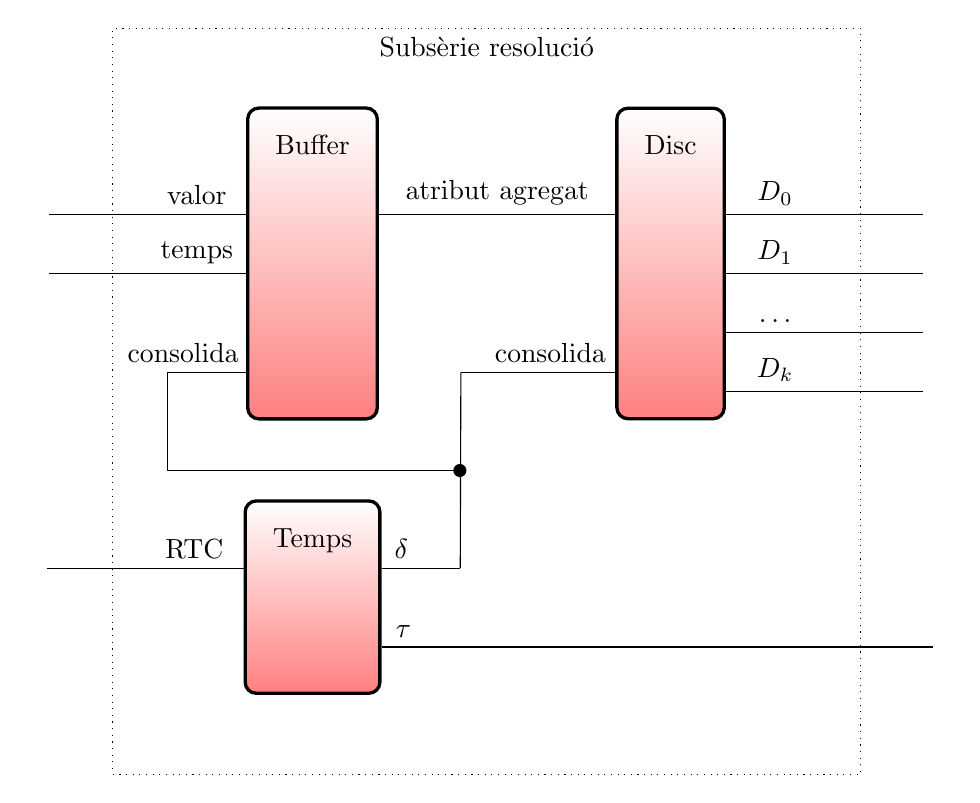
\begin{tikzpicture}
\tikzset{
    maquina/.style={rectangle,rounded corners,draw=black, 
      very thick, inner sep=1em, minimum size=3em, text centered,
      groc},
    interficie/.style={rectangle,rounded corners,draw=black, 
       inner sep=0.2em, minimum size=1em, text centered,
      verd},
    modul/.style={rectangle,rounded corners,draw=black, 
      very thick, inner sep=1em, minimum size=3em, text centered,
      roig},   
    myarrow/.style={->, >=latex', shorten >=1pt, thick},
    fletxaswitch/.style={<->, >=latex',shorten >=10pt,shorten <=10pt, thick},
    mylabel/.style={text width=7em, text centered},
    groc/.style={top color=white, bottom color=yellow!50},
    verd/.style={top color=white, bottom color=green!50},
    roig/.style={top color=white, bottom color=red!50},
  }  

  
   \node (discres) [draw, dotted, minimum width=9.5cm, text depth=9cm, rectangle] {Subsèrie resolució};



  \node[modul,text depth=3cm,below right=1cm and 1.7cm of discres.north west] (buffer) {Buffer};  

  %entrades
  \node[above left=-1.5cm and 2.5cm of buffer.north west] (buffer_valor)   {};
  \draw[-] (buffer_valor) -- (buffer_valor-|buffer.west)
   node[near end,above]{valor};

   \node[below=0.5cm of buffer_valor] (buffer_nou)   {};
   \draw[-] (buffer_nou) -- (buffer_nou-|buffer.west)
   node[near end,above]{temps};

   \node[above left=-3.5cm and 1cm of buffer.north west] (buffer_consolida) {};
   \draw[-] (buffer_consolida) -- (buffer_consolida-|buffer.west)
   node[pos=0.2,above]{consolida};

   %sortides
   \node[above right=-1.5cm and 1.5cm of buffer.north east] (buffer_dada)   {};
  \draw[-] (buffer_dada) -- (buffer_dada-|buffer.east)
   node[pos=0,above]{atribut agregat};





  \node[modul,right=3cm of buffer,text depth=3cm] (disc)   {Disc}; 

  % entrades
  \node[above left=-1.5cm and 2cm of disc.north west] (disc_valor)   {};
  \draw[-] (disc_valor) -- (disc_valor-|disc.west)
   node[near end,above]{};

  \node[above left=-3.5cm and 1.96cm of disc.north west] (disc_consolida)   {};
  \draw[-] (disc_consolida) -- (disc_consolida-|disc.west)
   node[pos=0.58,above]{consolida};

   % sortides
   \node[above right=-1.5cm and 2.5cm of disc.north east] (disc_d0)   {};
   \draw[-] (disc_d0) -- (disc_d0-|disc.east)
   node[near end,above]{$D_0$};

   \node[below=0.5cm of disc_d0] (disc_d1)   {};
  \draw[-] (disc_d1) -- (disc_d1-|disc.east)
   node[near end,above]{$D_1$};

   \node[below=0.5cm of disc_d1] (disc_d2)   {};
  \draw[-] (disc_d2) -- (disc_d2-|disc.east)
   node[near end,above]{$\dots$};

   \node[below=0.5cm of disc_d2] (disc_d3)   {};
  \draw[-] (disc_d3) -- (disc_d3-|disc.east)
   node[near end,above]{$D_k$};




  \node[modul,below=1cm of buffer,text depth=1.5cm] (temps)   {Temps}; 

  % entrades
  \node[above left=-1cm and 2.5cm of temps.north west] (temps_rtc)   {};
  \draw[-] (temps_rtc) -- (temps_rtc-|temps.west)
   node[near end,above]{RTC};

  % sortides
   \node[above right=-1cm and 1cm of temps.north east] (temps_delta)   {};
   \draw[-] (temps_delta) -- (temps_delta-|temps.east)
   node[near end,above]{$\delta$};

   \node[above right=-2cm and 7cm of temps.north east] (temps_tau)   {};
   \draw[-] (temps_tau) -- (temps_tau-|temps.east)
   node[pos=0.96,above]{$\tau$};








   %connexions
   \draw[-] (temps_delta.west) -- (disc_consolida.east); 
   
%   \node[above left=0.3cm and 1cm of temps.north west] (tau_reset)   {};
   \node[below=1cm of buffer_consolida] (tau_reset)   {};
   \draw[-*,shorten >=-2pt] (tau_reset) -- (tau_reset-|disc_consolida.east);
   \draw[-] (tau_reset.east) -- (tau_reset.east|-buffer_consolida);


 \end{tikzpicture}
 
\caption{Esquema d'integració d'una subsèrie resolució}
\label{fig:vhdl:resolucio}
\end{figure}

En aquesta implementació només fem referència a la part
d'emmagatzematge.  Caldria implementar un protocol per tal de
consultar les dades emmagatzemades, si bé forma senzilla es podria
implementar com si els discs fossin un perifèric de memòria.  

% Podrien ser emmagatzematges volàtils depenent de la criticitat de les dades



Algunes aplicacions dels sistemes integrats de multiresolució podrien ser:

\begin{itemize}
\item Emmagatzematge de la multiresolució en perifèrics la informació
  dels quals, tot i no ser essencial,  pot ajudar a monitorar-ne el seu
  funcionament. Per exemple comptadors d'aparells de xarxa,
  temperatures dels components, etc.

\item Aparells integrats molt petits, en els quals hi ha molt poc
  espai per a l'emmagatzematge. %en materials molt prims i doblegables.

\item Com un complement més de sensors inte\l.ligents, que actualment
  ja integren diverses tasques: filtratge del senyal, busos de
  comunicacions, llindars d'alarma, etc.


\item Per a computar funcions d'agregació d'atributs complexes. En
  aquest cas els buffers podrien treballar directament amb components
  del maquinari. Per exemple per a agregacions de sèries temporals en
  què els valors fossin imatges.

\item Implementació de la multiresolució en Field Programmable Gate
  Arrays, és a dir en dispositius de maquinari configurables. Això
  permetria major flexibilitat a l'hora de canviar els esquemes de
  multiresolució integrats.



\end{itemize}





% \subsection{RRDtool}

% \todo{fer}


% Ara hauríem de reprendre RRDtool i avaluar fins a quin punt compleix el nostre model. 
% Segur que hi ha punts en què no compleix... 

% Podem dir que RRDtool és la implementació productiva que actualment més s'apropa al concepte de multiresolució que hem formalitzat.


% Regarding other implementations,
% % \emph{RRDtool} can be seen as an specific case of \acro{MTSMS} and as
% % a NoSQL system, although Oetiker \cite{rrdtool} has not commented
% % it. However, regardless of the implementation backend, we have shown
% % how a generic model for \acro{MTSMS} can be defined firmly rooted on
% % \acro{DBMS} algebra theory.






% % RRDtool té una estructura multiresolució amb un buffer únic d'entrada
% % i buffers orientats a stream; segons havíem avaluat anteriorment \parencite{llusa11:tfm}.


% % S'ha d'estudiar com es fan les consultes a RRDtool

% % \url{http://en.wikipedia.org/wiki/RRD_Editor}



% % Podem considerar que:

% % 1. RRDtool és un SGBD NoSQL?
% % 2. Nosaltres n'hem formalitzat un model lògic?
% % 3. És el primer model lògic per a un producte NoSQL?
% % 4. Aquest model lògic es pot implementar tant en productes relacionals com amb NoSQL? i per tant es demostra que els models lògics són extremadament potents i necessaris?
% % 5. La implementació que fa RRDtool és molt eficient per a un determinat camp d'aplicació?
% % 6. La implementació relacional seria molt genèrica i propera al model però no tan eficient? més aviat subjecte a l'eficiència genèrica dels SGBDR?
% % 7. Els SGST són uns SGBD més simples? no tenen tantes actualitzacions de valors, no hi ha tantes relationships en l'esquema... Els SGST només es preocupen de sèries temporals i per tant només d'un tipus de dades en concret, això no obstant tal com s'ha dissenyat el model aquest tipus de dades es pot implementar en SGBD més complexos. 

% Hi ha RRDtool, que és un SGBD específic dissenyat per a dades monitorades. Les causes del seu disseny són:

% * Tobias Oetiker dissenyava un monitor de paràmetres de xarxes de comunicacions i en aquest monitor una part era la d'emmagatzematge de les dades. Per raons pràctiques i d'utilitat dissenya aquesta part amb un esquema inovadós. Finalment acaba separant aquesta part i la converteix independentment en RRDtool.

% * RRDtool té aquest model pràctic i a la pràctica és molt útil per a ser usat com a SGBD dels sistemes de monitoratge, sobretot en l'àmbit dels comptadors de xarxa on és l'estàndard de facto. 

% Això no obstant, no hi ha cap raonament teòric sobre el model de RRDtool ja que s'ha dissenyat per raons pràctiques. Per tant, entendre el funcionament de RRDtool és complicat, hi ha un nivell molt elevat per començar a fer-lo funcionar i molts conceptes no s'entenen perquè no estan ben definits. 

% Per això ens proposem de compendre i formalitzar el model de RRDtool, que acabarem anomenar model de multiresolució, en la teoria dels sitemes d'informació. A més RRDtool és molt específic pel camp de comptadors de xarxa i volem oferir un model genèric per a altres àmbits.  









\section{Reflexions sobre la qualitat}


El capítol d'aplicació de la teoria de la informació és una
introducció al problema de la qualitat de la multiresolució.  La
teoria de la informació formalitza anàlisis més profundes per a la
compressió de dades que es podrien aplicar també a la multiresolució.
En el cas que es conegui més bé el context i el comportament de la
sèrie temporal a la qual s'aplica la multiresolució, es pot detallar
més bé la quantificació de l'error. Aleshores, en termes de la teoria
de la informació, hi ha més coneixement sobre la predicció
del comportament de les dades cosa que es pot utilitzar per a avaluar
característiques més concretes. Per exemple, una variable real
adquirida té limitat el rang de valors que pot prendre i fins i tot
pot tenir un comportament probabilístic determinat.



Cal notar que no avaluem la idoneïtat d'aplicar un estadístic o un
altre a unes dades. Altrament, ja partim del cas que es vol aplicar
una consulta amb una agregació determinada a una sèrie temporal.
Per a determinar un esquema de multiresolució --la quantitat de
resolucions, els passos de consolidació de cadascuna, els cardinals,
\dots-- caldria analitzar cada problema particular en el seu context i
utilitzar els coneixements adequats. Per exemple, per a treballar amb
problemes de so la teoria del senyal formalitza tot de raonaments que
no es poden obviar a l'hora de definir-ne un esquema de
multiresolució.  O bé, també en la teoria del senyal, es poden trobar
anàlisis per a determinar bons passos de consolidació per a una
variable, per exemple de temperatura. Així i tot, en el cas dels
comptadors se'n pot fer un raonament a banda per a conservar la seva
informació genuïna de comptatge lligada a com l'adquireixen.


A partir de les reflexions fetes sobre la qualitat de la
multiresolució s'obren un seguit de qüestions més, cadascuna de les
quals és un repte futur:
\begin{itemize}
\item Quina redundància d'emmagatzematge hi ha entre diverses
  subsèries d'una mateixa sèrie temporal multiresolució? Què ocorre
  quan hi ha més d'una resolució i són de diferents funcions
  d'agregació d'atributs?

\item En cas que es perdi una resolució, es podria reconstruir a
  partir de les altres? O bé en cas que es vulgui ampliar la mida d'un
  disc, es podria completar amb les dades d'altres resolucions?

\item Les resolucions encadenades són interessant perquè aprofiten les
  dades emmagatzemades però afegeixen més restriccions a la compressió
  d'informació. Com es poden barrejar diferents passos de consolidació
  i diferents funcions d'agregació d'atributs?


\item Gràcies a un esquema de multiresolució es pot emmagatzemar dades
  d'una sèrie temporals durant un llarg temps de forma
  comprimida. Aquesta durada de temps és llarga però finita, tot i que
  quan s'esgoti dinàmicament es pot afegir una nova subsèrie amb
  inferior resolució però amb més lapse. Inicialment aquesta subsèrie
  serà buida, però es podria utilitzar les dades ja emmagatzemades per
  a iniciar-la?

\end{itemize}




















% \subsubsection{Operacions habituals en les sèries temporals}


% \paragraph{Semblança de dues sèries temporals}


% Similarity Measures for Time Series

% Hi ha varis mètodes, [keogh08:vldb] n'avalua uns quants i els generalitza amb:

% Given two
% time series T1 and T2 , a similarity function Dist calcu-
% lates the distance between the two time series, denoted by
% Dist(T1 , T2 ).

% Exemplifiquem amb la distància euclídia, [keogh08:vldb] nota que és
% competitiva amb les altres.

% Distancia euclídia segons [faloutsous94-sigmod]


% \[
% D(S,Q) = \left( \sum_{i=1}^{l} (S[i]-Q[i])^2  \right)^{1/2}
% \]

% \begin{gather*}
%   D: S \times Q \longrightarrow v: \\
%   S' = map(fusio(S,Q),(t,v_1,v_2)\mapsto(t,(v_1-v_2)^2)), \\
%   S'' = fold(quad,(0,0),(t^1,v^1,t^2,v^2)\mapsto(t^1,v^1+v^2)), \\
%   v = \sqrt{V(m)}:m\in S''
% \end{gather*}


% S i Q haurien de ser regulars entre elles, sinó cal aplicar una fusió amb representació/interpretació.

% Amb la multiresolució la fusió es pot fer de forma eficient. Per altra banda, es podria crear un disc resolució amb agregador de semblança.


% \paragraph{Semblança de dues sèries temporals amb offset}

% Aquí es descriu la solució general del problema (SequentialScan),
% [faloutsous94-sigmod] n'estudia implementacions amb certes
% heurístiques que aconsegueixen més eficiència.





% \paragraph{Filtratge senzill per mitjana mòbil}

% Sigui $p$ la mida de la finestra mòbil
% \begin{gather*}
%   \text{MitMobil}: S \times \text{p} \longrightarrow S':\\
%   \text{map}(S,(t,v)\mapsto \text{mitjanaV}(S[t,t+p]))
% \end{gather*}


% Mitjana mòbil sobre la multiresolució



% \paragraph{Farciment de forats}

% Jo tinc una sèrie temporal i vull que entre dues mesures no hi hagi més d'un cert temps. Si no es compleix dic que té forats. 

% Sigui $S$ una sèrie temporal, aquesta té forats de més durada que $d$
% si alguna mesura compleix $\text{forats}(S,d) = \text{selecciona}(difT(S),v>d \bigwedge v\neq\infty)$ a on $difT(S) = \text{map}(\text{tpredecessors}(S),(t,v)\mapsto(t,t-v))$.

% Amb la multiresolució el farciment de forats és natural a l'estructura i és controlat per la funció agregadora d'atributs.


% * Com farciria els forats manualment a una sèrie temporal?

% 1. Passar-ho per un esquema de multiresolució

% 2. Treballar sobre la sèrie temporal:

% a partir del càlcul de forats anterior $\text{forats}(S,d)$ per
% exemple apliquem un farciment amb representació
% zohe. $\text{farciment}(S,d) = \text{unio}(S,S')$ a on fem la selecció
% de resolució $S' = S[T]^{\text{zohe}}$, $\forall (t,v) \in
% \text{forats}(S,d): T = \{ \tau = t - dn |
% \tau\in(t-v,t),n\in\mathbb{N} \}$.







% \subsubsection{Com treure profit de les operacions dels SGSTM}

% Temes que després es poden aprofitar a les implementacions

% * No hi ha updates --> les sèries temporals no s'han de canviar

% * Per exemple, vull calcular la mitjana de  BDSTM(a,b] si tinc un disc resolució amb $\delta=b-a$ i $f=$mitjana aquest seria l'adequat en comptes de calcular mitjana(SerieTotal(M)(a,b])

% %??
% % No obstant, la base de dades multiresolució conté informació sobre la
% % resolució de les subsèries i per tant aquesta operació és susceptible
% % d'implementar-se aprofitant aquesta informació.  A tall d'exemple es
% % defineix una operació per extreure de la base de dades multiresolució
% % una sèrie temporal regular amb període $T$:


% % \begin{definition}[Selecció de resolució regular]
% %   \begin{gather*}
% %     \text{ResolucióRegular}: M^* \times T \times r \longrightarrow S'\\
% %     \forall (S_{Bi},S_{Di},\delta_i,\tau_i,k_i,f_i) \in M : \\
% %     d_i = T - \delta_i , \\
% %     0 \geq d_0 > d_1 \dots > d_a, 0 < d_{a+1} < \dots < d_d: \\
% %     S'' = S_{D0} || S_{D1} || \dotsb || S_{Da}  ||  S_{Da+1} || \dotsb || S_{Dd}, \\
% %     S' = S''[i]^r: i = {t|0+nT,n\in\mathbb{N}}
% %   \end{gather*}
% % \end{definition}

% % Nota: les operacions no són equivalents, l'operació $\text{SerieTotal}(M)[i]^r$ és molt més potent que la $\text{ResolucióRegular}(M,T)$.




% \subsubsection{Semàntica de comportament}

% \todo{?}









%%% Local Variables:
%%% TeX-master: "main"
%%% End:
% LocalWords:  SGSTM multiresolució



%------- Annexos ------
%\appendix




\backmatter
\bookmarksetup{startatroot}%  per eliminar les parts
\addtocontents{toc}{\bigskip}% perhaps as well

%------- Bibliografia ------
\cleardoublepage
\phantomsection\addcontentsline{toc}{chapter}{\bibname}
%\pdfbookmark{\bibname}{bookmark:bibliografia}
\printbibliography
%----------------------------------------------


%------- Glossari ------
\cleardoublepage
%\phantomsection\addcontentsline{toc}{chapter}{\glossaryname}
%\pdfbookmark{\glossaryname}{bookmark:glossari}
\chapter{Abreviacions i nomenclatura}
\glsaddall[counter=subsection]
%\printglossary

\printglossary[type=abreviatura,nonumberlist]

\printglossary[type=\acronymtype,title=Sigles,nonumberlist]

\renewcommand{\glossarypreamble}{Índex de notació segons nom, símbol i
  referència --pàgina o en negreta lloc on es defineix el concepte:
  definició, secció (\S) o exemple (ex.). Organitzada en símbols
  matemàtics que requereixen aclariment i notació dels
  components dels \gls{SGST} i dels \gls{SGSTM}.}

\printglossary[type=notation,style=estil-notation]


%------------- Índexs ------------
%ATENCIÓ, hi ha problemes quan s'activen molts índexs
% \cleardoublepage\phantomsection\addcontentsline{toc}{chapter}{Índexs}\chapter*{Índexs}
% \begingroup
% \let\clearpage\relax
% \phantomsection\addcontentsline{toc}{section}{\listfigurename}\listoffigures
% %%%\cleardoublepage\phantomsection\addcontentsline{toc}{section}{\listtablename}\listoftables
% \phantomsection\addcontentsline{toc}{section}{\lstlistlistingname}\lstlistoflistings
% \renewcommand\listtheoremname{Índex de definicions}
% \phantomsection\addcontentsline{toc}{section}{\listtheoremname}\listoftheorems[ignoreall,show={definition}]
% \renewcommand\listtheoremname{Índex d'exemples}
% \phantomsection\addcontentsline{toc}{section}{\listtheoremname}\listoftheorems[ignoreall,show={example}]
% \endgroup
\listoftodos %%%%mode esborrany
%----------------------------------------------



\end{document}



%%%%%%%%%%%%%%%%%%%%%%%%%%%%%%%%%%%%%%%%%%%%%%%%%%%%%%%%%%%%%%%%%%%%%%%%%%  
% Memòria Tesi Doctoral. 
%
% Copyright (C) 2011-2014 Aleix Llusà Serra.
% 
% This LaTeX document is free software: you can redistribute it and/or
% modify it under the terms of the GNU General Public License as
% published by the Free Software Foundation, either version 3 of the
% License, or (at your option) any later version.
%
% This document is distributed in the hope that it will be useful, but
% WITHOUT ANY WARRANTY; without even the implied warranty of
% MERCHANTABILITY or FITNESS FOR A PARTICULAR PURPOSE. See the GNU
% General Public License for more details.
%
% You should have received a copy of the GNU General Public License
% along with this document. If not, see <http://www.gnu.org/licenses/>.
%
%
% Aleix Llusà Serra
% Departament de Disseny i Programació de Sistemes Electrònics de la Universitat Politècnica de Catalunya (DiPSE-UPC)
% Escola Politècnica Superior d'Enginyeria de Manresa (EPSEM)
% Av. de les Bases de Manresa, 61-73
% 08242 Manresa (Barcelona)
% PAÏSOS CATALANS 
%
% aleix (a) dipse.upc.edu
% 
% El codi font LaTeX del document es troba a 
% <http://escriny.epsem.upc.edu/projects/rrb/>
%%%%%%%%%%%%%%%%%%%%%%%%%%%%%%%%%%%%%%%%%%%%%%%%%%%%%%%%%%%%%%%%%%%%%%%%%% 